\documentclass[a4paper]{article}
\usepackage{header}

\begin{document}
    \begin{flushright}
      \textit{Лекции по линейной алгебре 1 курс БПМИ 2017/2018}
      
      \textit{Левина Александра}
    \end{flushright}

    \tableofcontents

    \newpage

    \section{Лекция 09.09.2019}
\subsection{Матрицы}
\begin{definition}
    \textit{Матрица размера $n \times m$} --- это прямоугольная таблица высоты $m$ и ширины $n$.
\end{definition}

\begin{equation*}
    A = \begin{pmatrix}
        a_{11}  & a_{12} & \dots & a_{1n} \\
        a_{21} & a_{22} & \dots & a_{2n} \\
        \vdots & \vdots & \ddots & \vdots \\
        a_{m1} & a_{m2} & \dots & a_{mn}
    \end{pmatrix}
\end{equation*}

$a_{ij}$ -- элемент на пересечении $i$-й строки и $j$-го столбца

Краткая запись -- $A = (a_{ij})$

Множество всех матриц размера $m \times n$ с коэффициентами из $\RR$ (множество всех действительных чисел) --- $\text{Mat}_{n \times m}(\RR)$ или $\text{Mat}_{n \times m}$

\begin{definition}
    Две матрицы $A \in \text{Mat}_{n \times m}$ и $B \in \text{Mat}_{p \times q}$ называются \textit{равными}, если $m = p$, $n = q$, и соответствующие элементы равны
\end{definition}

\begin{example}
    $\begin{pmatrix}
       \circ & \circ & \circ \\ \circ & \circ & \circ
    \end{pmatrix}
    \neq
    \begin{pmatrix}
        \circ & \circ \\ \circ & \circ \\ \circ & \circ
    \end{pmatrix}$
\end{example}

\subsection{Операции над матрицами}

Для любых $A, B \in \text{Mat}_{m \times n}$

\begin{itemize}
    \item \emph{Сложение} $A + B := (a_{ij} + b_{ij})$
    \item \emph{Умножение на скаляр} $\alpha \in \RR \implies \lambda A := (\lambda a_{ij})$
\end{itemize}

\textbf{Свойства суммы и произведения на скаляр}

$\forall A, B, C  \in \text{Mat}_{m \times n} \quad \forall \lambda, \mu \in \RR$
\begin{enumerate}[label=\arabic*), nosep]
    \item $A + B = B + A$ (коммутативность)

    \item $(A + B) + C = A + (B + C)$ (ассоциативность)

    \item $A + 0 = 0 + A = A$, где 
        \begin{equation*}
            0 = \begin{pmatrix}
                0 & 0 & \dots & 0 \\
                0 & 0 & \dots & 0 \\
                \vdots & \vdots & \ddots & \vdots \\
                0 & 0 & \dots & 0
            \end{pmatrix} \text{ --- нулевая матрица}
        .\end{equation*}

    \item $A + (-A) = 0$
    
        $-A = (-a_{ij})$ -- противоположная матрица

    \item $(\lambda + \mu) A = \lambda A + \mu A$

    \item $\lambda (A + B) = \lambda A + \lambda B$

    \item $\lambda (\mu A) = \lambda (\mu A)$

    \item $1 A = A$
\end{enumerate}

\bigskip
\textit{\textbf{Упражнение на дом.} Доказать эти свойства.}

\begin{comment}
    Из свойств 1) -- 8) следует, что $\text{Mat}_{n \times m}(\RR)$ является векторным пространством над \( \RR \)
\end{comment}


\subsection{Пространство $\RR^n$, его отождествление с матрицами-столбцами высоты $n$}

\noindent
$\RR^n := \{(x_1, \dots, x_n) \mid x_i \in \RR \ \forall i = 1, \dots, n \}$
\begin{description}[nosep]
\item[$\RR^1$] -- числовая прямая
\item[$\RR^2$] -- плоскость
\item[$\RR^3$] -- трехмерное пространство
\end{description}

\bigskip
Договоримся отождествлять \( \RR^n \) со столбцами высоты \( n \)

$(x_1, \dots, x_n) \leftrightarrow \begin{pmatrix} x_1 \\ \vdots \\ x_n \end{pmatrix}$ -- \textit{вектор столбец}

$\RR^n = \left\{\begin{pmatrix} x_1 \\ x_2 \\ \vdots \\ x_n \end{pmatrix} \mid x \in \RR \ \forall i = 1, \dots, n \right\} = \text{Mat}_{n \times 1}(\RR)$

$\left[ x = \begin{pmatrix}
    x_1 \\ \vdots \\ x_n
\end{pmatrix} \in \RR^n, y = \begin{pmatrix}
    y_1 \\ \vdots \\ y_n
\end{pmatrix} \in \RR^n \right] \implies 
\left[ x = y \iff x_i = y_i \ \forall i \right]$

\( x + y := \begin{pmatrix}
    x_1 + y_1 \\ \vdots \\ x_n + y_n
\end{pmatrix} \)

$\lambda \in \RR \implies \lambda x_i := (\lambda x_1, \dots, \lambda x_n)$


\subsection{Транспонирование матриц, его простейшие свойства}

$A \in \text{Mat}_{m \times n} = \begin{pmatrix}
    a_{11} & a_{12} & \dots & a_{1n} \\
    a_{21} & a_{22} & \dots & a_{2n} \\
    \vdots & \vdots & \ddots & \vdots \\
    a_{m1} & a_{m2} & \dots & a_{mn}
\end{pmatrix} \leadsto A^T \in \text{Mat}_{n \times m} := \begin{pmatrix}
    a_{11} & a_{21} & \dots & a_{m1} \\
    a_{12} & a_{22} & \dots & a_{m2} \\
    \vdots & \vdots & \ddots & \vdots \\
    a_{1n} & a_{2n} & \dots & a_{mn}
\end{pmatrix}$

$A^T$ ---  \textit{транспонированная матрица}

\bigskip
Свойства:
\begin{enumerate}[label=\arabic*), nosep]
    \item $(A^T)^T = A$
    \item $(A + B)^T = A^T + B^T$
    \item $(\lambda A)^T = \lambda A^T$
\end{enumerate}

\begin{example}
    \( \begin{pmatrix}
        x_1 & \dots & x_n
    \end{pmatrix}^T = \begin{pmatrix}
        x_1 \\ \vdots \\ x_n
    \end{pmatrix} \)
\end{example}
\begin{example}
    \( \begin{pmatrix}
    x_1 \\ \vdots \\ x_n
    \end{pmatrix}^T = \begin{pmatrix}
    x_1 & \dots & x_n
    \end{pmatrix} \)
\end{example}
\begin{example}
    \( \begin{pmatrix}
        1 & 2 \\ 3 & 4 \\ 5 & 6
    \end{pmatrix}^T = \begin{pmatrix}
        1 & 3 & 5 \\
        2 & 4 & 6
    \end{pmatrix} \)
\end{example}

\subsection{Умножение матриц}

Пусть $A = (a_{ij}) \in \text{Mat}_{m \times n}$

\bigskip

$A_{(i)} = \begin{pmatrix} a_{i1}, a_{i2}, \dots, a_{in} \end{pmatrix} $ --- $i$-я строка матрицы $A$

$A^{(j)} = \begin{pmatrix} a_{1j} \\ a_{2j} \\ \vdots \\ a_{mn} \end{pmatrix} $ --- $j$-й  столбец матрицы $A$

\begin{enumerate}[label=\arabic*)]
    \item 
        Частный случай: умножение строки на столбец той же длинны
    
        $\underbrace{(x_1, \dots, x_n)}_{1 \times n} 
        \underbrace{\begin{pmatrix}
            x_1 \\ \vdots \\ x_n
        \end{pmatrix}}_{n \times 1} 
        = x_1 \cdot y_1 + \dots + x_n \cdot y_n$
        
    \item
        Общий случай:

        $A$ - матрица размера $m \times \underline{n}$
        
        $B$ - матрица размера $\underline{n} \times p$
        
        Кол-во строк матрицы $A$ равно количеству столбцов матрицы $B$ --- условие согласованности матриц
        
        $AB := C \in \text{Mat}_{m \times p}$, где $C_{ij} = A_{(i)} B^{(j)}$
\end{enumerate}

\begin{example}
    \( \begin{pmatrix}
        y_1 \\ \vdots \\ y_n
    \end{pmatrix} 
    \begin{pmatrix}
        x_1 & \dots & x_n
    \end{pmatrix}
    := 
    \begin{pmatrix}
        x_1 y_1 & x_2 y_1 & \dots & x_n y_1 \\
        x_1 y_2 & x_2 y_2 & \dots & x_n y_2 \\
        \vdots & \vdots & \ddots & \vdots \\
        x_1 y_n & x_2 y_m & \dots & x_n y_m 
    \end{pmatrix} \)
\end{example}

\begin{example}
    $\begin{pmatrix}
        1 & 0 & 2 \\
        0 & -1 & 3
    \end{pmatrix}
    \times
    \begin{pmatrix}
        2 & -1 \\
        0 & 5 \\
        1 & 1
    \end{pmatrix}
    =
    \begin{pmatrix}
        1 \cdot 2 + 0 \cdot 0 + 2 \cdot 1 & 1 \cdot (-1) + 0 \cdot 5 + 2 \cdot 1 \\
        0 \cdot 2 + (-1) \cdot 0 + 3 \cdot 1 & 0 \cdot (-1) + (-1) \cdot 5 + 3 \cdot 1
    \end{pmatrix}
    =
    \begin{pmatrix}
        4 & 1 \\
        3 & -2
    \end{pmatrix}$
\end{example}

    \section{Лекция 12.09.2019 \\ Основные свойства умножения матриц. Система линейных уравнений}

\subsection{Отступление о суммах}

Пусть $S_p, S_{p + 1}, \dots, S_q$ -- набор чисел.

\bigskip
Тогда, $\sum_{i = p}^q S_i := S_p + S_{p + 1} + \dots + S_q $ -- сумма по $i$ от $p$ до $q$

\bigskip
Например, $\sum_{i=1}^{100} i^2 = 1^2 + 2^2 + \dots + 100^2$

\bigskip
\textbf{Свойства сумм}:
\begin{enumerate}
    \item $\lambda \sum_{i=1}^n S_i = \sum_{i=1}^n \lambda S_i $
    \item $\sum_{i=1}^n (S_i + T_i) = \sum_{i=1}^n S_i + \sum^n_{i=1} T_i $
    \item $\sum_{i=1}^m \sum_{j=1}^n S_{ij} = \sum_{j=1}^n \sum_{i=1}^m S_{ij}$ --- сумма всех элементов матрицы $S = (S_{ij})$
\end{enumerate}

\subsection{Свойства умножения матриц}

Пусть $A \in \text{Mat}_{m \times n}, \ B \in \text{Mat}_{n \times p}$

\begin{enumerate}
\item 
    $\underbracket{A(B + C)}_x = \underbracket{AB + AC}_y$ --- левая дистрибутивность.
   
    \begin{proof}
        \begin{align*}
            x_{ij} = A_{(i)} (B + C)^{(j)} 
            &= \sum_{k = 1}^{n} a_{ik} (b_{kj} + c_{kj}) \\
            &= \sum_{k = 1}^{n} (a_{ik} b_{kj} + a_{ik} c_{kj}) \\
            &= \sum_{k = 1}^{n} a_{ik} b_{kj} + \sum_{k = 1}^{n} a_{ik} c_{kj} \\
            &= A_{(i)} B^{(j)} + A_{(i)} C^{(j)} = y_{ij}
        .\end{align*}
    \end{proof}

\item $(A+B)C = AC + BC$ --- правая дистрибутивность, доказывается аналогично.

\item $\lambda(AB) = (\lambda A) B = A (\lambda B)$

\item $(AB)C = A(BC)$ --- ассоциативность.

    \begin{proof}
        $\underbracket{(AB)}_u C = x, A\underbracket{(BC)}_v = y$

        \begin{align*}
            x_{ij} 
            &= \sum_{k = 1}^{n} u_{ik} \cdot c_{kj}
            = \sum_{k = 1}^{n} \left(\sum_{l = 1}^{p} a_{il} b_{lk}\right) c_{kj}
            = \sum_{k = 1}^{n} \sum_{l = 1}^{p} \left(a_{il} b_{lk} c_{kj}\right) \\
            &= \sum_{l = 1}^{p} \sum_{k = 1}^{n} \left(a_{il} b_{lk} c_{kj}\right)
            = \sum_{l = 1}^{p} a_{il} \sum_{k = 1}^{n} \left(b_{lk} c_{kj}\right)
            = \sum_{l = 1}^{p} a_{il} v_{lj} = y_{ij}
        .\end{align*}
    \end{proof}

\item 
    $\underbracket{(AB)^T}_x = \underbracket{B^T A^T}_y$
   
    \begin{proof}
            $x_{ij} = [AB]_{ji} = A_{(j)} B^{(i)} = B^T_{(i)} (A^T)^{(j)} = y_{ij}$
    \end{proof}
\end{enumerate}

Умножение матриц не коммутативно

$A = \begin{pmatrix} 0 & 1 \\ 0 & 0 \end{pmatrix}, 
B = \begin{pmatrix} 0 & 0 \\ 1 & 0 \end{pmatrix}$

$AB = \begin{pmatrix}1 & 0 \\ 0 & 0\end{pmatrix}, 
BA = \begin{pmatrix}0 & 0 \\ 0 & 1\end{pmatrix}$

\bigskip
\begin{definition}
    $A \in \text{Mat}_{n \times n}$ называется \textit{квадртаной матрицей} порядка $n$
\end{definition}

Обозначение $M_n := \text{Mat}_{n \times n}$

$A \in M_n$

\bigskip
\begin{definition}
    Матрица $A \in M_n$ называется \textit{диагональной} если все ее элементы вне главной диагонали равны нулю ($a_{ij} = 0$ при $i \neq j$)
\end{definition}

\begin{equation*}
    A = \begin{pmatrix} 
        a_1 & 0 & \dots & 0 \\
        0 & a_2 & \dots & 0 \\
        \vdots & \vdots & \ddots & \vdots \\
        0 & 0 & \dots & a_n
    \end{pmatrix} \implies A = \diag(a_1, a_2, \dots, a_n)
.\end{equation*}

\begin{lemma}
    $A = diag(a_1, \dots, a_n) \in M_n \implies$
    \begin{enumerate}
    \item $\forall B \in \text{Mat}_{n \times p} \implies AB = \begin{pmatrix}
            a_1 B_{(1)} \\
            a_2 B_{(2)} \\
            \vdots \\
            a_n B_{(n)} 
        \end{pmatrix}$
    \item $\forall B \in \text{Mat}_{m \times n} \implies BA = \begin{pmatrix} 
            a_1 B^{(1)} & a_2 B^{(2)} & \dots & a_n B^{(n)}
        \end{pmatrix}$ 
    \end{enumerate}
\end{lemma}

\begin{proof}
    \begin{enumerate}
    \item $[AB]_{ij} = \begin{pmatrix} 0 & \dots & 0 & a_i & 0 & \dots & 0\end{pmatrix} \begin{pmatrix} b_{1j} \\ b_{2j} \\ \vdots \\ b_{nj} \end{pmatrix} = a_i b_{ij} $
    \item $[BA]_{ij} = \begin{pmatrix} b_{i1} & b_{i2} & \dots & b_{im} \end{pmatrix} \begin{pmatrix} \vdots \\ 0 \\ a_j \\ 0 \\ \vdots \end{pmatrix} = b_{ij} a_j$ 
    \end{enumerate}
\end{proof}

\begin{definition}
    Матрица $E = E_n = diag(1, 1, \dots, 1)$ называется \textit{единичной матрицей} порядка $n$. 

    \begin{equation*}
        E = \begin{pmatrix} 
            1 & 0 & \dots & 0 \\
            0 & 1 & \dots & 0 \\
            \vdots & \vdots & \ddots & \vdots \\
            0 & 0 & \dots & 1
        \end{pmatrix} 
    \end{equation*}
\end{definition}

\textbf{Свойства}:
\begin{enumerate}
    \item $EA = A \quad \forall A \in \text{Mat}_{n \times p}$
    \item $AE = A \quad \forall A \in \text{Mat}_{p \times n}$
    \item $AE = EA = A \quad \forall A \in M_n$
\end{enumerate}

\begin{definition}
    \textit{Следом} матрицы $A \in M_n$ называется число $trA = a_{11} + a_{22} + \dots + a_{nn} = \sum_{i=1}^n a_{ii}$ 
\end{definition}

\textbf{Свойства}:
\begin{enumerate}
\item $\tr(A + B) = \tr A + \tr B$
\item $\tr \lambda A = \lambda \tr A$
\item $\tr A^T = \tr A$
\item $\tr(AB) = \tr(BA)$

    $\forall A \in \text{Mat}_{m \times n}, B \in \text{Mat}_{n \times m}$

    \begin{proof}
        $AB = x \in M_m$, $BA = y \in M_n$

        \begin{align*}
            \tr x 
            = \sum_{i = 1}^{m} x_{ii} 
            &= \sum_{i = 1}^{m} \sum_{j = 1}^{n} \left(a_{ij} b_{ji}\right) \\
            &= \sum_{j = 1}^{n} \sum_{i = 1}^{m} \left(b_{ji} a_{ij}\right) 
            = \sum_{j = 1}^{n} y_{jj} 
            = \tr y
        .\end{align*}
    \end{proof}
\end{enumerate}

\begin{example}
    $A = (1, 2, 3), B = \begin{pmatrix}4 \\ 5 \\ 6\end{pmatrix}$

    $tr(AB) = tr(1 \cdot 4 + 2 \cdot 5 + 3 \cdot 6) = 32$

    $tr(BA) = \tr \begin{pmatrix} 4 & 8 & 12 \\ 5 & 10 & 15 \\ 6 & 12 & 18 \end{pmatrix} = 4 + 10 + 18 = 32$
\end{example}


\subsection{Системы линейных уравнений.}

\textit{Линейное уравнение}: $a_1 x_1 + \dots + a_n x_n = b$.

$a_1, a_2, \dots, a_n, b \in \RR$ -- коэффициенты.

$x_1, x_2, \dots, x_n$ -- неизвестные.

\bigskip
Система линейных уравнений (СЛУ):
\begin{equation*}
    \begin{cases}
        \begin{aligned}
            a_{11} x_1 + a_{12} x_2 + \cdots + a_{1n} x_n &= b_1 \\
            a_{21} x_1 + a_{22} x_2 + \cdots + a_{2n} x_n &= b_2 \\
            \hdotsfor{2} \\
            a_{m1} x_1 + a_{m2} x_2 + \cdots + a_{mn} x_n &= b_m \\
        \end{aligned}
    \end{cases}
\end{equation*}
m уравнений, n неизвестных

\begin{definition}~
    \begin{enumerate}
    \item \textit{Решение одного уравнения} -- это такой набор значений неизвестных $x_1, x_2, \dots, x_n$, при подстановке которого в уравнение получаем тождество.
    \item \textit{Решение СЛУ} -- такой набор значений неизвестных, который является решением каждого уравнения СЛУ.
    \end{enumerate}
\end{definition}

Основная задача: решить СЛУ, т.е. найти все решения.

\bigskip
\begin{example}

    $n = m = 1$

    $ax = b$, $a, b \in \RR$, x -- неизвестная

    \begin{enumerate}
    \item $a \neq 0 \implies x = \frac{b}{a}$ -- единственное

    \item $a = 0 \implies 0x = b$

        $b \neq 0 \implies$ решений нет.

        $b = 0 \implies x$ -- любое $\implies$ бесконечно много решений.
    \end{enumerate}
\end{example}

\begin{definition}
    СЛУ называется 

    -- \textit{совместной}, если у нее есть хотя бы одно решение

    -- \textit{несовместной}, если решений нет
\end{definition}

\subsubsection*{Матричная форма записи СЛУ}

$AX = B$.
\begin{equation*}
    A \in Mat_{m \times n}(R) = \begin{pmatrix}
        a_{11} & a_{12} & \dots & a_{1n} \\
        a_{21} & a_{22} & \dots & a_{2n} \\
        \vdots & \vdots & \ddots & \vdots \\
        a_{m1} & a_{m2} & \dots & a_{mn}
    \end{pmatrix} \text{ -- матрица коэффициентов}
\end{equation*}

\begin{equation*}
    B \in \text{Mat}_{m \times 1} = \begin{pmatrix}
        b_1 \\ b_2 \\ \vdots \\ b_n
    \end{pmatrix} \text{ -- столбец правых частей}
\end{equation*}

\begin{equation*}
    X \in \text{Mat}_{m \times 1} = \begin{pmatrix}
        x_1 \\ x_2 \\ \vdots \\ x_n
    \end{pmatrix} \text{ -- столбец неизвестных}
\end{equation*} 

    \section{Лекция 14.09.2019}

\subsection{Расширенная матрицы системы линейных уравнений}

$Ax = b$, $A \in \text{Mat}_{m \times n}$, $b \in \RR^m$

Полная информация о СЛУ содержится в её \textit{расширенной матрице}.
\begin{equation*}
    \begin{pmatrix} A \mid b \end{pmatrix} = \begin{amatrix}{4}{1}
    a_{11} & a_{12} & \dots & a_{1n} & b_1 \\
    a_{21} & a_{22} & \dots & a_{2n} & b_2 \\
    \vdots & \vdots & \ddots & \vdots \\
    a_{m1} & a_{m2} & \dots & a_{mn} & b_m
    \end{amatrix}
\end{equation*}

\subsection{Эквивалентные системы}
\begin{definition}
    Две системы уравнений от одних и тех же неизвестных называются \textit{эквивалентными}, если они имеют одинаковые множества решений.
\end{definition}

\begin{example}
    Рассмотрим несколько СЛУ

    \begin{enumerate}[label=\Alph*)]
    \item
        $\begin{cases}
            x_1 + x_2 = 1 \\
            x_1 - x_2 = 0
        \end{cases} \iff \begin{amatrix}{2}{1}
            1 & 1 & 1 \\
            1 & -1 & 0
        \end{amatrix}$

    \item
        $\begin{cases}
            2x_1 = 1 \\
            2x_2 = 1
        \end{cases} \iff \begin{amatrix}{2}{1}
            2 & 0 & 1 \\
            0 & 2 & 1
        \end{amatrix}$

    \item
        $x_1 + x_2 = 1 \iff \begin{amatrix}{2}{1} 1 & 1 & 1 \end{amatrix}$
    \end{enumerate}

    A и B эквиваленты, так как обе имеют единственное решение $\left(\frac{1}{2}, \frac{1}{2}\right)$.
    
    A и C не эквивалентны, так как C имеет бесконечно много решений.
\end{example}

\subsection{Как решить СЛУ?}

\textbf{Идея}: выполнить преобразование СЛУ, сохраняющее множество её решений, и привести её к такому виду, в котором СЛУ легко решается.

\begin{example}
    $\begin{pmatrix}
        1 & 0 & \dots & 0 \\
        0 & 1 & \dots & 0 \\
        \vdots & \vdots & \ddots & \vdots \\
        0 & 0 & \dots & 1
    \end{pmatrix} \leftrightarrow \begin{cases}
        x_1 = b_1 \\
        x_2 = b_2 \\ 
        \vdots \\ 
        x_n = b_n
    \end{cases}$
\end{example}

\subsubsection{Элементарные преобразования СЛУ и соответствующие преобразования строк её расширенной матрицы}

\begin{tabular}{c|c|c}
    тип & СЛУ & расширенная матрица \\
    \hline
    1. & K $i$-му уравнению прибавить $j$-ое, умноженное на $\lambda \in \RR \ (i \neq j)$ & $\text{Э}_1(i, j, \lambda)$ \\
    2. & Переставить $i$-е и $j$-е уравнения $(i \neq j)$ & $\text{Э}_2(i, j)$ \\
    3. & Умножить $i$-ое уравнение на $\lambda \neq 0$ & $\text{Э}_3(i, \lambda)$
\end{tabular}

\begin{enumerate}
\item
    $\text{Э}_1(i, j, \lambda)$: к $i$-ой строке прибавить $j$-ую, умноженную на $\lambda$ (покомпонентно), 

    $a_{ik} \mapsto a_{ik} + \lambda a_{jk} \ \forall k = 1, \dots, n$,
    
    $b_i \mapsto b_i + \lambda b_j$.
    
\item
    $\text{Э}_2(i, j)$: переставить i-ую и j-ую строки.

\item
    $\text{Э}_3(i, \lambda)$: умножить i-ю строку на $\lambda$ (покомпонентно).
\end{enumerate}

$\text{Э}_1, \text{Э}_2, \text{Э}_3$ называются \textit{элементарными преобразованиями строк расширенной матрицы}.


\subsubsection{Сохранение множества решений системы линейных уравнений при элементарных преобразованиях}
\begin{lemma}
    Элементарные преобразования СЛУ не меняют множество решений
\end{lemma}

\begin{proof}
    Пусть мы получили СЛУ$(\star\star)$ из СЛУ($\star$) путем применения элементарных преобразований.

    \begin{enumerate}[nosep]
    \item
        Всякое решение системы $(\star)$ является решением $(\star\star)$.
    \item
        $(\star)$ получается из $(\star\star)$ путем элементарных преобразований.

        \begin{tabular}{c|c|}
            $(\star) \to (\star\star)$ & $(\star\star) \to (\star)$ \\
            \hline
            $\text{Э}_1(i, j, \lambda)$ & $\text{Э}_1(i, j, -\lambda)$ \\
            $\text{Э}_2(i, j)$ & $\text{Э}_2(i, j)$ \\
            $\text{Э}_3(i, \lambda)$ & $\text{Э}_3(i, \frac{1}{\lambda})$
        \end{tabular}
    \end{enumerate} 

    Следовательно, всякое решение ($\star\star$) является решением ($\star$) $\implies$ множества решений совпадают.
\end{proof}


\subsection{Ступенчатые матрицы}

\begin{definition}
    Строка $(a_1, a_2, \dots, a_n)$ называется \textit{нулевой}, если $a_1 = a_2 = \dots = a_n = 0$ и \textit{ненулевой} иначе ($\exists i : a_i \neq 0$).
\end{definition}

\begin{definition}
    \textit{Ведущим элементом} ненулевой строки называется первый её ненулевой элемент.
\end{definition}

\begin{definition}
    Матрица $M \in \text{Mat}_{m \times n}$ называется \textit{ступенчатой}, или имеет ступенчатый вид, если:
    \begin{enumerate}
    \item Номера ведущих элементов её ненулевых строк строго возрастают.
    \item Все нулевые строки стоят в конце.
    \end{enumerate}
\end{definition}
\begin{equation*}
    M = \begin{pmatrix}
        0 & \dots & 0 & \diamond & * & * & * & * & * & * \\
        0 & \dots & 0 & 0 & \dots & \diamond & * & * & * & * \\
        0 & \dots & 0 & 0 & \dots & 0 & 0 & \diamond & * & * \\
        \vdots & \ddots & \vdots & \vdots & \ddots & \vdots & \vdots & \vdots & \vdots & \vdots \\
        0 & \dots & 0 & 0 & \dots & 0 & 0 & 0 & \diamond & * \\
        0 & \dots & 0 & 0 & \dots & 0 & 0 & 0 & 0 & \diamond \\
        0 & \dots & 0 & 0 & \dots & 0 & 0 & 0 & 0 & 0
    \end{pmatrix}
,\end{equation*}
где $\diamond \neq 0$, $*$ -- что угодно. 


\subsubsection{Улучшенный ступенчатый вид матрицы}
\begin{definition}
    M имеет \textit{улучшенный ступенчатый вид}, если:

    \begin{enumerate}[nosep]
    \item M имеет обычный ступенчатый вид.
    \item Все ведущие элементы равны 1.
    \item В одном столбце с любым ведущим элементом стоят только нули.
    \end{enumerate}
\end{definition}

\begin{equation*}
    M = \begin{pmatrix}
        0 & \dots & 0 & 1 & * & 0 & * & 0 & 0 & * \\
        0 & \dots & 0 & 0 & \dots & 1 & * & 0 & 0 & * \\
        0 & \dots & 0 & 0 & \dots & 0 & 0 & 1 & 0 & * \\
        \vdots & \vdots & \vdots & \vdots & \vdots & \vdots & \vdots & \vdots & \vdots & \vdots \\
        0 & 0 & 0 & \dots & \dots & \dots & \dots & 0 & 1 & * \\
        0 & 0 & 0 & \dots & 0 & 0 & 0 & 0 & 0 & 0
    \end{pmatrix}
.\end{equation*}

\begin{theorem}
    \begin{enumerate}[label=\arabic*),nosep]
    \item Всякую матрицу элементарными преобразованиями можно привести к ступенчатому виду. 
    \item Всякую ступенчатую матрицу элементарными преобразованиями строк можно привести к улучшенному ступенчатому виду.
    \end{enumerate}
\end{theorem}

\begin{corollary}
    Всякую матрицу элементарными преобразованиями строк можно привести к \textbf{улучшенному} ступенчатому виду.
\end{corollary}

\begin{proof}~
    \begin{enumerate}
    \item
        Алгоритм. Если M - нулевая, то конец. Иначе:
        \begin{enumerate}[label=Шаг \arabic*:]
        \item Ищем первый ненулевой столбец, пусть $j$ --- его номер.
        \item Переставляем строки, если нужно, добиваемся того, что $a_{1j} \neq 0$
        \item 
            Зануляем элементы в этом столбце используя первую строку --  $\text{Э}_1(2, 1, -\frac{a_{2j}}{a_{1j}}), \dots, \text{Э}_1(m, 1, -\frac{a_{mj}}{a_{1j}})$.

            В результате $a_{ij} = 0$ при $i = 2, 3, \dots m$.
        \end{enumerate}
        Дальше повторяем все шаги для подматрицы $M'$ (без первой строки и столбцов $1, \dots, j$).
    \item 
        Алгоритм. Пусть $a_{1j_1}, a_{2j_2}, \dots, a_{rj_r}$ -- ведущие элементы ступенчатой матрицы.
        \begin{enumerate}[label=Шаг \arabic*:]
        \item Выполняем $\text{Э}_3(1, \frac{1}{a_{1j_1}}), \dots, \text{Э}_3(r, \frac{1}{a_{rj_r}})$, в результате все ведущие элементы равны 1.
        \item Выполняем $\text{Э}_1(r - 1, r, -a_{r - 1, \; j_r}), \text{Э}_1(r - 2, r, -a_{r - 2, \; j_r}), \dots, \text{Э}_1(1, r, -a_{1, \; j_r})$. В результате все элементы над $a_{r j_r}$ равны 0.
            
            Аналогично обнуляем элементы над всеми остальными ведущими.
        \end{enumerate}
    \end{enumerate}
    Итог: матрица имеет улучшенный ступенчатый вид.
\end{proof}


\subsection{Реализация элементарных преобразований строк матрицы при помощи умножения слева на подходящую матрицу}

Всякое элементарное преобразование строк матрицы реализуется умножением как умножение слева на подходящую ``элементарную матрицу''.

\begin{itemize}
\item 
    $\text{Э}_1(i, j, \lambda)$: $A \mapsto U_1(i, j, \lambda)A$, где
    \begin{equation*}
        U_1(i, j, \lambda) = \bordermatrix{
            &   &   &   &   &   & j &   \cr
            & 1 & 0 & 0 & \dots & 0 & 0 & 0 \cr
          i & 0 & 1 & 0 & \dots & 0 & \lambda & 0 \cr
            & 0 & 0 & 1 & \dots & 0 & 0 & 0 \cr
            & \vdots & \vdots & \vdots & \ddots & \vdots & \vdots & \vdots \cr
            & 0 & 0 & 0 & \dots & 1 & 0 & 0 \cr
            & 0 & 0 & 0 & \dots & 0 & 1 & 0 \cr
            & 0 & 0 & 0 & \dots & 0 & 0 & 1
        }
    \end{equation*}

    (на диагонали стоят единицы, на $i$-м $j$-м месте стоит $\lambda$, остальные элементы нули)

\item

    $\text{Э}_2(i, j)$: $A \mapsto U_2(i, j)A$, где
    \begin{equation*}
        U_2(i, j) = \bordermatrix{
            &   & i &   &   &   & j &   \cr
            & 1 & 0 & 0 & \dots & 0 & 0 & 0 \cr
          i & 0 & 0 & 0 & \dots & 0 & 1 & 0 \cr
            & 0 & 0 & 1 & \dots & 0 & 0 & 0 \cr
            & \vdots & \vdots & \vdots & \ddots & \vdots & \vdots & \vdots \cr
            & 0 & 0 & 0 & \dots & 1 & 0 & 0 \cr
          j & 0 & 1 & 0 & \dots & 0 & 0 & 0 \cr
            & 0 & 0 & 0 & \dots & 0 & 0 & 1
        }
    \end{equation*}

    (на диагонали стоят единицы, кроме $i$-го и $j$-го столбца (на $i$-м $j$-м и $j$-м $i$-м местах стоит 1, остальные нули)

\item 
    $\text{Э}_3(i, \lambda)$: $A \mapsto U_3(i, \lambda)A$, где
    \begin{equation*}
        U_3(i, \lambda) = \bordermatrix{    
            &   & i &   &   &   &   &   \cr
            & 1 & 0 & 0 & \dots & 0 & 0 & 0 \cr
          i & 0 & \lambda & 0 & \dots & 0 & 0 & 0 \cr
            & 0 & 0 & 1 & \dots & 0 & 0 & 0 \cr
            & \vdots & \vdots & \vdots & \ddots & \vdots & \vdots & \vdots \cr
            & 0 & 0 & 0 & \dots & 1 & 0 & 0 \cr
            & 0 & 0 & 0 & \dots & 0 & 1 & 0 \cr
            & 0 & 0 & 0 & \dots & 0 & 0 & 1
        }
    \end{equation*}

    (на диагонали стоят единицы, кроме i-го столбца, там $\lambda$, остальные элементы нули)
\end{itemize}

Элементарные преобразования столбцов --- умножение на соответствующую матрицу справа.

\bigskip
\textit{\textbf{Упражнение на дом.}} Доказательство.

    \section{Лекция 7.09.2017}
\subsection{Системы линейных уравнений.}

Линейное уравнение: $a_1 x_1 + \cdots + a_n x_n = b$.

$a_1, a_2, \cdots, a_n, b \in \mathbb{R}$ -- заданные числа.

$x_1, x_2, \cdots, x_n$ -- неизвестные.

\vspace{\baselineskip}
Система линейных уравнений (СЛУ):
\[
	\left\{
		\begin{aligned}
        a_{11}x_1 + a_{12}x_2 + \cdots + a_{1n}x = b_1 \\
        a_{21}x_1 + a_{22}x_2 + \cdots + a_{2n}x = b_2 \\
        \hdots \hdots \hdots \hdots \hdots \hdots \hdots \hdots \hdots \hdots\\
        a_{m1}x_1 + a_{m2}x_2 + \cdots + a_{mn}x = b_m \\
		\end{aligned}
	\right.
\]
m уравнений, n неизвестных

\vspace{\baselineskip}
\textbf{Определение.} 1) \textit{Решение одного уравнения} -- это такой набор значений неизвестных $x_1, x_2, \cdots, x_n$, при подстановке которого в уравнение получаем тождество.

2) \textit{Решение СЛУ} -- такой набор значений неизвестных, который является решением каждого уравнения СЛУ.

\vspace{\baselineskip}
Основная задача: решить СЛУ, т.е. найти все решения.

\vspace{\baselineskip}
Пример. $n = m = 1$

$ax = b$, $a, b \in \mathbb{R}$, x - неизвестная

1) $a \neq 0 \Rightarrow x = \frac{b}{a}$ -- единственное

2) $a = 0 \Rightarrow 0x = b$

$b \neq 0 \Rightarrow$ решений нет.

$b = 0 \Rightarrow$ x - любое $\Rightarrow$ бесконечно много решений.

\vspace{\baselineskip}
\textbf{Определение.} СЛУ называется \textit{совместной}, если у нее есть решение. СЛУ называется \textit{несовместной}, если у нее решений нет.

\vspace{\baselineskip}
\textbf{Определение.} Две СЛУ от одних и тех же неизвестных называются \textit{эквивалетными}, когда у них совпадают множества решений.

\vspace{\baselineskip}
Примеры.

1) Любые две несовместные СЛУ эквивалентны, т.к. множество решений пусто.

2) 
\[
	\left\{
		\begin{aligned}
        x_1 + x_2 = 1 \\
        x_1 - x_2 = 0
		\end{aligned}
	\right. 
\]
\[
    \left\{
		\begin{aligned}
        2x_1 = 1 \\
        2x_2 = 1
		\end{aligned}
	\right.
\]
Эквивалентные множества решений: $ \left\{ \left( \frac{1}{2} ; \frac{1}{2} \right) \right\}$.

\vspace{\baselineskip}
Как решить СЛУ?

\textit{Идея:} выполнить преобразования СЛУ, не меняющие множество решениq, и привести ее в итоге к виду, в котором она легко решается.

\[
	\begin{pmatrix}
		a_{11} & a_{12} & \cdots & a_{1n} & \vrule & b_1 \\
		a_{21} & a_{22} & \cdots & a_{2n} & \vrule & b_2 \\
       \vdots & \vdots & \vdots& \vdots & \vrule & \vdots\\ 
       a_{m1} & a_{m2} & \cdots & a_{mn} & \vrule & b_m
	\end{pmatrix}
    =
    \begin{pmatrix}
    	A & \vrule & b
	\end{pmatrix}
\]

-- расширенная матрица СЛУ (*), она содержит в себе всю информацию о СЛУ(*), где 

\[
	\begin{pmatrix}
		a_{11} & a_{12} & \cdots & a_{1n} \\
		a_{21} & a_{22} & \cdots & a_{2n} \\
       \vdots & \vdots & \vdots& \vdots \\ 
       a_{m1} & a_{m2} & \cdots & a_{mn}
	\end{pmatrix}
    = A
\]

-- матрица коэффициентов,

\[
	\begin{pmatrix}
		b_1 \\
        b_2 \\
        \vdots \\
        b_m
	\end{pmatrix}
    = b
\]

-- столбец правых частей.

\vspace{\baselineskip}
В примерах выше:

1) 
\[
	\begin{pmatrix}
		1 & 1 & \vrule & 1 \\
        1 & -1 & \vrule & 0 
	\end{pmatrix}
\]

\[
	\begin{pmatrix}
		2 & 0 & \vrule & 1 \\
        0 & 2 & \vrule & 1 
	\end{pmatrix}
\]

\vspace{\baselineskip}
2) Пример простого вида:

\[
	\begin{pmatrix}
		1 & 0 & 0 & \cdots & 0 & \vrule & b_1 \\
		0 & 1 & 0 & \cdots & 0 & \vrule & b_2 \\
        0 & 0 & 1 & \cdots & 0 & \vrule & b_3 \\
        \cdots & \cdots & \cdots & \cdots & \cdots & \vrule & \cdots \\
        0 & 0 & 0 & \cdots & 1 & \vrule & b_m 
	\end{pmatrix}
\]

соответсвующая СЛУ:

\[
    \left\{
		\begin{aligned}
        x_1 = b_1 \\
        x_2 = b_2 \\
        \vdots \\
        x_m = b_m
		\end{aligned}
	\right.
\]

\subsection{Элементарные преобразования СЛУ и ее расширенная матрица.}

\vspace{\baselineskip}
\begin{table}[!ht]
		\begin{tabular}{c|c|c}
    	тип & СЛУ & расширенная матрица \\
        \hline
        1. тип & К i-му уравнению прибавить j-ое, умноженное на $\lambda \in \mathbb{R} (i \neq j)$ & $Э_1$(i, j, $\lambda$) \\
        2. тип & Переставить i-е и j-е уравнения $(i \neq j)$  & $Э_2$(i, j) \\
        3. тип & Умножить i-ое уравнение на $\lambda \neq 0$ & $Э_3$(i, $\lambda$) 
		\end{tabular}
\end{table}

\vspace{\baselineskip}
1) $Э_1$(i, j, $\lambda$): к i-ой строке прибавить j-ую, умноженную на $\lambda$ (покомпонентно),

$a_{ik} \rightarrow a_ik + \lambda a_{jk} \forall k = 1, \cdots, n$,

$b_i \rightarrow b_i + \lambda b_j$.

2) $Э_2$(i, j): переставить i-ю и j-ю строки.

3) $Э_3$(i, $\lambda$): умножить i-ю строку на $\lambda$ (покомпоненто).

\vspace{\baselineskip}
$Э_1$, $Э_2$, $Э_3$ называются \textit{элементарными преобразованиями строк расширенной матрицы}.

\vspace{\baselineskip}
\textbf{Лемма.} Элементарные преобразования СЛУ не меняют множество решений.

\vspace{\baselineskip}
\textbf{\textit{Доказательство.}} Пусть мы получили СЛУ(**) из СЛУ(*) путем элементарных преобразований.

$\rhd$ 1) всякое решение СЛУ(*) является решением СЛУ(**);

2) СЛУ(*) тоже получается из СЛУ(**) путем элементарных преобразований

\begin{table}[!ht]
	\begin{center}
		\begin{tabular}{c|c|c}
    	(*) $\rightarrow$ (**) & (**) $\rightarrow$ (*) \\
        \hline
        $Э_1$(i, j, $\lambda$) & $Э_1$(i, j, $-\lambda$)\\
        $Э_2$(i, j) & $Э_2$(i, j)\\
        $Э_3$(i, $\lambda$) & $Э_3$(i, $\frac{1}{\lambda}$)
		\end{tabular}
	\end{center}
\end{table}

\vspace{\baselineskip}
1) $\Rightarrow$ всякое решение СЛУ(**) является решением СЛУ(*) $\Rightarrow$ (*) и (**) имеют одно и то же множество решений. $\lhd$


    \section{Лекция 21.09.2017}

\subsection{}
M - матрица.

\vspace{\baselineskip}
\textbf{Определение.} Строка ($a_1, a_2, \dots , a_n$) называется \textit{нулевой}, если $a_1 = a_2 = \dots = a_n = 0$ , и \textit{ненулевой} иначе (т.е. $\exists i: a_i \neq 0$).

\vspace{\baselineskip}
\textbf{Определение.} \textit{Ведущий элемент} ненулевой строки -- это первый ненулевой элемент этой строки.

\vspace{\baselineskip}
\textbf{Определение.} Матрица М называется \textit{ступенчатой} (имеет \textit{ступенчатый вид}), если:

1) номера ведущих элементов ненулевых строк строго возратают;

2) все нулевые строки в конце (= внизу).

\[
    \begin{pmatrix}
    	0 & \cdots & 0 & \Diamond & * & * & * & * & * & * \\
        0 & \cdots & 0 & 0 & \cdots & \Diamond & * & * & * & * \\
        0 & \cdots & 0 & 0 & \cdots & 0 & 0 & \Diamond & * & * \\
        \vdots & \vdots & \vdots& \vdots & \vdots & \vdots & \vdots & \vdots & \vdots& \vdots \\
        0 & 0 & 0 & \cdots & \cdots & \cdots & \cdots & 0 & \Diamond & *\\
        0 & 0 & 0 & \cdots & 0 & 0 & 0 & 0 & 0 & 0
	\end{pmatrix}
\]

$\Diamond \neq 0$

$*$ -- что угодно

\vspace{\baselineskip}
\textbf{Определение.} Матрица М имеет \textit{улучшенный ступенчатый вид}, если:

1) М имеет ступенчатый вид;

2) все ведущие элементы $ = 1$;

3) в одном столбце с каждым ведущим элементом стоят только нули.

\[
	\begin{pmatrix}
    	0 & \cdots & 0 & 1 & * & 0 & * & 0 & 0 & * \\
        0 & \cdots & 0 & 0 & \cdots & 1 & * & 0 & 0 & * \\
        0 & \cdots & 0 & 0 & \cdots & 0 & 0 & 1 & 0 & * \\
        \vdots & \vdots & \vdots& \vdots & \vdots & \vdots & \vdots & \vdots & \vdots& \vdots \\
        0 & 0 & 0 & \cdots & \cdots & \cdots & \cdots & 0 & 1 & *\\
        0 & 0 & 0 & \cdots & 0 & 0 & 0 & 0 & 0 & 0
	\end{pmatrix}
\]

\begin{theorem}[]\label{theorem1}
	1) Всякую матрицу элементарными преобразованиями строк можно привести к ступенчатому виду.

2) Всякую ступенчатую матрицу элементарными преобразованиями строк можно привести к улучшенному ступенчатому виду.
\end{theorem}

\begin{corollary}
	Всякую матрицу элементарными преобразованиями строк можно привести к ступенчатому виду.
\end{corollary}

\begin{comment}
	Улучшенный ступенчатый вид матрицы определен однозначно.
\end{comment}

\textbf{\textit{Доказательство теоремы.}} 

$\rhd$ Обозначения: m - число строк, n - число столбцов, $a_{ij}$ - элемент, стоящий на пересечении i-ой стhоки и j-ого столбца.

\vspace{\baselineskip}
1) Алгоритм. Если М -- нулевая, то конец. Иначе:

\textit{Шаг 1.} Ищем первый ненулевой столбец, пусть j -- его номер.

\textit{Шаг 2.} Переставляя строки, если нужно, добиваемся того, что $a_{1j} \neq 0 $

\textit{Шаг 3.} Выполняем $Э_1$(2,1,$-\frac{a_{2j}}{a_{1j}}$), $\dots$, $Э_1$(m,1,$-\frac{a_{mj}}{a_{1j}}$). В результате $a_{ij} = 0$ при $i = 2,3, \dots, m$. 

Дальше все повторяем для меньшей матрицы М'.

\vspace{\baselineskip}
2) Алгоритм. Пусть $a_{1j_1}, a_{2j_2}, \dots, a_{rj_r}$ -- ведущие элементы ступенчатой матрицы.

\textit{Шаг 1.} Выполняем $Э_3$(1,$\frac{1}{a_{1j_1}}$), \dots, $Э_3$(r,$\frac{1}{a_{rj_r}}$), в результате все ведущие элементы равны 1.

\textit{Шаг 2.} Выполнив $Э_1$(r-1, r, $-a_{{r-1}\ j_r}$), $Э_1$(r-2, r, $-a_{{r-2}\ j_r}$), $\dots$, $Э_1$(1, r, $-a_{1\ j_r}$). В результате все элементы над $a_{rj_r}$ равны 0.

Аналогично обнуляем элементы над всеми остальными ведущими. 

Итог: матрица имеет улучшеный ступенчатый вид. $\lhd$

\vspace{\baselineskip}
\subsection{Метод Гаусса решения СЛУ (метод исключения неизвестных).}

Пусть есть СЛУ с расширенной матрицей (A|b): m уравнений, n неизвестных. Помним: элементарные преобразования строк расширенной матрицы не меняют множество решений.

Алгоритм. Приводим (A|b) к ступенчатому виду (прямой ход метода Гаусса). Получаем: 

\[
	\begin{pmatrix}
		0 & \cdots & 0 & a_{1j_1} & \cdots & \cdots & \cdots & \vrule & b_1 \\
		0 & \cdots & 0 & 0 & a_{2j_2} & \cdots & \cdots & \vrule & b_2 \\
       \vdots & \vdots & \vdots& \vdots & \vdots & \vdots & \vdots & \vrule & \vdots & \\ 
       0 & 0 & 0 & \cdots & 0 & 0 & a_{rj_r} & \vrule & b_r \\
       0 & 0 & 0 & \cdots & 0 & 0 & 0 & \vrule & b_{r+1} \\
       0 & 0 & 0 & \cdots & 0 & 0 & 0 & \vrule & 0
	\end{pmatrix}
\]


\textit{Случай 1.} $b_{r+1} \neq 0$. Тогда новая СЛУ содержит уравнение $0*x_1 + \dots + 0*x_n = b_{r+1}$ ($\Leftrightarrow 0 = b_{r+1}$) $\Rightarrow$ СЛУ несовместна.

\textit{Случай 2.} Либо $r = m$, либо $b_{r+1} = 0$. Приводим матрицу к улучшенному ступенчатому виду (обратный ход метода Гаусса).
\[
	\bordermatrix{ 
    	 & & & & j_1 & j_2 & & j_r & \cr
    	 & 0 & \cdots & 0 & 1 & \cdots & \cdots & \cdots & \vrule & b_1 \cr
		 & 0 & \cdots & 0 & 0 & 1 & \cdots & \cdots & \vrule & b_2 \cr
        & \vdots & \vdots & \vdots& \vdots & \vdots & \vdots & \vdots & \vrule & \vdots & \cr 
        & 0 & 0 & 0 & \cdots & 0 & 0 & 1 & \vrule & b_r \cr
        & 0 & 0 & 0 & \cdots & 0 & 0 & 0 & \vrule & 0 \cr
        & 0 & 0 & 0 & \cdots & 0 & 0 & 0 & \vrule & 0}
\]

Неизвестные $x_{j_1}, x_{j_2}, \dots , x_{j_r}$ называются \textit{главными}, а остальные -- \textit{свободными}.

\vspace{\baselineskip}
\textit{Подслучай 2.1.} $r = n$, т. е. все неизвестные -- главные.

\[
	\begin{pmatrix}
		1 & \cdots & 0 & \vrule & b_1 \\
        \cdots & \ddots & \cdots & \vrule & \cdots \\
        0 & \cdots & 1 & \vrule & b_r \\
       0 & \cdots & 0 & \vrule & 0 \\
       0 & \cdots & 0 & \vrule & 0
	\end{pmatrix}
\]

Тогда СЛУ имеет вид: 

\[
	\left\{
		\begin{aligned}
        x_1 = b_1 \\
        x_2 = b_2 \\
        \cdots \\
        x_n = b_n
		\end{aligned}
	\right.
\]

-- единственное решение.

\vspace{\baselineskip}
\textit{Подслучай 2.2.} $r < n$, т.е. хотя бы одна свободная неизвестная.

Перенося в каждом уравнении члены со свободными неизвестными в правую часть, получаем выражения всех главных неизвестных через свободные, эти выражения называются \textit{общим решением исходной СЛУ}.

Каждое решение исходной СЛУ получается подстановкой произвольных значений в свободные неизвестные и вычислением соответсвующих значений главных неизвестных.

\begin{comment}
	И тогда СЛУ имеет бесконечно много решений.
\end{comment}

Пример. Улучшенный ступенчатый вид: 

\[
	\begin{pmatrix}
		1 & 3 & 0 & 1 & \vrule & -1 \\
		0 & 0 & 1 & -2 & \vrule & 4
	\end{pmatrix}
\]

Главные неизвестные: $x_1, x_3$

Свободные неизвестные: $x_2, x_4$.

$x_2 = t_1, x_4 = t2$ -- параметры.

\[
	\begin{pmatrix}
    x_1 \\
    x_2 \\
    x_3 \\
    x_4
	\end{pmatrix}
    =
    \begin{pmatrix}
    -1 - 3t_1 - t_2 \\
    t_1 \\
    4 + 2t_2 \\
    t_2
    \end{pmatrix}
    =
    \begin{pmatrix}
    -1\\
    0\\
    4\\
    0
    \end{pmatrix}
    + t_1
    \begin{pmatrix}
    -3\\
    1\\
    0\\
    0
    \end{pmatrix}
    +t_2
    \begin{pmatrix}
    -1\\
    0\\
    2\\
    1
    \end{pmatrix}
\]

Общее решение:

\[
	\left\{
		\begin{aligned}
        x_1 = -1 - 3x_2 - x_4\\
        x_3 = 4 + 2x_4 \\
		\end{aligned}
	\right.
\]

\begin{corollary}
Всякая СЛУ с коэффициентами из $\mathbb{R}$ либо несовместна, либо имеет ровно 1 решение, либо имеет бесконечно много решений.
\end{corollary}

\textbf{Определение.} СЛУ называется \textit{однородной} (ОСЛУ), если все ее правые части равны 0. Расширенная: (A|0). 

\vspace{\baselineskip}
\textbf{Очевидный факт:} всякая ОСЛУ имеет нулевое решение ($x_1 = x_2 = \cdots= x_n = 0$).

\begin{corollary}
Всякая ОСЛУ либо имеет ровно 1 решение (нулевое), либо бесконечно много решений.
\end{corollary}

\begin{corollary}
Всякая ОСЛУ, у которой число неизвестных больше числа уравнений, имеет ненулевое решение.
\end{corollary}

\textbf{\textit{Доказательство:}} 

$\rhd$ В ступенчатом виде расширенной матрице ступенек будет $\le m$ (m -- количество уравнений). Число ступенек = числу главных неизвестных $\Rightarrow$ главных неизвестных $\le m$ $\Rightarrow$ будет хотя бы одна свободная неизвестная. Подставляя в свободную неизвестную ненулевое значение, получим ненулевое решение. $\lhd$


    \section{Лекция 14.09.2019}

\subsection{Расширенная матрицы системы линейных уравнений}

$Ax = b$, $A \in \text{Mat}_{m \times n}$, $b \in \RR^m$

Полная информация о СЛУ содержится в её \textit{расширенной матрице}.
\begin{equation*}
    \begin{pmatrix} A \mid b \end{pmatrix} = \begin{amatrix}{4}{1}
    a_{11} & a_{12} & \dots & a_{1n} & b_1 \\
    a_{21} & a_{22} & \dots & a_{2n} & b_2 \\
    \vdots & \vdots & \ddots & \vdots \\
    a_{m1} & a_{m2} & \dots & a_{mn} & b_m
    \end{amatrix}
\end{equation*}

\subsection{Эквивалентные системы}
\begin{definition}
    Две системы уравнений от одних и тех же неизвестных называются \textit{эквивалентными}, если они имеют одинаковые множества решений.
\end{definition}

\begin{example}
    Рассмотрим несколько СЛУ

    \begin{enumerate}[label=\Alph*)]
    \item
        $\begin{cases}
            x_1 + x_2 = 1 \\
            x_1 - x_2 = 0
        \end{cases} \iff \begin{amatrix}{2}{1}
            1 & 1 & 1 \\
            1 & -1 & 0
        \end{amatrix}$

    \item
        $\begin{cases}
            2x_1 = 1 \\
            2x_2 = 1
        \end{cases} \iff \begin{amatrix}{2}{1}
            2 & 0 & 1 \\
            0 & 2 & 1
        \end{amatrix}$

    \item
        $x_1 + x_2 = 1 \iff \begin{amatrix}{2}{1} 1 & 1 & 1 \end{amatrix}$
    \end{enumerate}

    A и B эквиваленты, так как обе имеют единственное решение $\left(\frac{1}{2}, \frac{1}{2}\right)$.
    
    A и C не эквивалентны, так как C имеет бесконечно много решений.
\end{example}

\subsection{Как решить СЛУ?}

\textbf{Идея}: выполнить преобразование СЛУ, сохраняющее множество её решений, и привести её к такому виду, в котором СЛУ легко решается.

\begin{example}
    $\begin{pmatrix}
        1 & 0 & \dots & 0 \\
        0 & 1 & \dots & 0 \\
        \vdots & \vdots & \ddots & \vdots \\
        0 & 0 & \dots & 1
    \end{pmatrix} \leftrightarrow \begin{cases}
        x_1 = b_1 \\
        x_2 = b_2 \\ 
        \vdots \\ 
        x_n = b_n
    \end{cases}$
\end{example}

\subsubsection{Элементарные преобразования СЛУ и соответствующие преобразования строк её расширенной матрицы}

\begin{tabular}{c|c|c}
    тип & СЛУ & расширенная матрица \\
    \hline
    1. & K $i$-му уравнению прибавить $j$-ое, умноженное на $\lambda \in \RR \ (i \neq j)$ & $\text{Э}_1(i, j, \lambda)$ \\
    2. & Переставить $i$-е и $j$-е уравнения $(i \neq j)$ & $\text{Э}_2(i, j)$ \\
    3. & Умножить $i$-ое уравнение на $\lambda \neq 0$ & $\text{Э}_3(i, \lambda)$
\end{tabular}

\begin{enumerate}
\item
    $\text{Э}_1(i, j, \lambda)$: к $i$-ой строке прибавить $j$-ую, умноженную на $\lambda$ (покомпонентно), 

    $a_{ik} \mapsto a_{ik} + \lambda a_{jk} \ \forall k = 1, \dots, n$,
    
    $b_i \mapsto b_i + \lambda b_j$.
    
\item
    $\text{Э}_2(i, j)$: переставить i-ую и j-ую строки.

\item
    $\text{Э}_3(i, \lambda)$: умножить i-ю строку на $\lambda$ (покомпонентно).
\end{enumerate}

$\text{Э}_1, \text{Э}_2, \text{Э}_3$ называются \textit{элементарными преобразованиями строк расширенной матрицы}.


\subsubsection{Сохранение множества решений системы линейных уравнений при элементарных преобразованиях}
\begin{lemma}
    Элементарные преобразования СЛУ не меняют множество решений
\end{lemma}

\begin{proof}
    Пусть мы получили СЛУ$(\star\star)$ из СЛУ($\star$) путем применения элементарных преобразований.

    \begin{enumerate}[nosep]
    \item
        Всякое решение системы $(\star)$ является решением $(\star\star)$.
    \item
        $(\star)$ получается из $(\star\star)$ путем элементарных преобразований.

        \begin{tabular}{c|c|}
            $(\star) \to (\star\star)$ & $(\star\star) \to (\star)$ \\
            \hline
            $\text{Э}_1(i, j, \lambda)$ & $\text{Э}_1(i, j, -\lambda)$ \\
            $\text{Э}_2(i, j)$ & $\text{Э}_2(i, j)$ \\
            $\text{Э}_3(i, \lambda)$ & $\text{Э}_3(i, \frac{1}{\lambda})$
        \end{tabular}
    \end{enumerate} 

    Следовательно, всякое решение ($\star\star$) является решением ($\star$) $\implies$ множества решений совпадают.
\end{proof}


\subsection{Ступенчатые матрицы}

\begin{definition}
    Строка $(a_1, a_2, \dots, a_n)$ называется \textit{нулевой}, если $a_1 = a_2 = \dots = a_n = 0$ и \textit{ненулевой} иначе ($\exists i : a_i \neq 0$).
\end{definition}

\begin{definition}
    \textit{Ведущим элементом} ненулевой строки называется первый её ненулевой элемент.
\end{definition}

\begin{definition}
    Матрица $M \in \text{Mat}_{m \times n}$ называется \textit{ступенчатой}, или имеет ступенчатый вид, если:
    \begin{enumerate}
    \item Номера ведущих элементов её ненулевых строк строго возрастают.
    \item Все нулевые строки стоят в конце.
    \end{enumerate}
\end{definition}
\begin{equation*}
    M = \begin{pmatrix}
        0 & \dots & 0 & \diamond & * & * & * & * & * & * \\
        0 & \dots & 0 & 0 & \dots & \diamond & * & * & * & * \\
        0 & \dots & 0 & 0 & \dots & 0 & 0 & \diamond & * & * \\
        \vdots & \ddots & \vdots & \vdots & \ddots & \vdots & \vdots & \vdots & \vdots & \vdots \\
        0 & \dots & 0 & 0 & \dots & 0 & 0 & 0 & \diamond & * \\
        0 & \dots & 0 & 0 & \dots & 0 & 0 & 0 & 0 & \diamond \\
        0 & \dots & 0 & 0 & \dots & 0 & 0 & 0 & 0 & 0
    \end{pmatrix}
,\end{equation*}
где $\diamond \neq 0$, $*$ -- что угодно. 


\subsubsection{Улучшенный ступенчатый вид матрицы}
\begin{definition}
    M имеет \textit{улучшенный ступенчатый вид}, если:

    \begin{enumerate}[nosep]
    \item M имеет обычный ступенчатый вид.
    \item Все ведущие элементы равны 1.
    \item В одном столбце с любым ведущим элементом стоят только нули.
    \end{enumerate}
\end{definition}

\begin{equation*}
    M = \begin{pmatrix}
        0 & \dots & 0 & 1 & * & 0 & * & 0 & 0 & * \\
        0 & \dots & 0 & 0 & \dots & 1 & * & 0 & 0 & * \\
        0 & \dots & 0 & 0 & \dots & 0 & 0 & 1 & 0 & * \\
        \vdots & \vdots & \vdots & \vdots & \vdots & \vdots & \vdots & \vdots & \vdots & \vdots \\
        0 & 0 & 0 & \dots & \dots & \dots & \dots & 0 & 1 & * \\
        0 & 0 & 0 & \dots & 0 & 0 & 0 & 0 & 0 & 0
    \end{pmatrix}
.\end{equation*}

\begin{theorem}
    \begin{enumerate}[label=\arabic*),nosep]
    \item Всякую матрицу элементарными преобразованиями можно привести к ступенчатому виду. 
    \item Всякую ступенчатую матрицу элементарными преобразованиями строк можно привести к улучшенному ступенчатому виду.
    \end{enumerate}
\end{theorem}

\begin{corollary}
    Всякую матрицу элементарными преобразованиями строк можно привести к \textbf{улучшенному} ступенчатому виду.
\end{corollary}

\begin{proof}~
    \begin{enumerate}
    \item
        Алгоритм. Если M - нулевая, то конец. Иначе:
        \begin{enumerate}[label=Шаг \arabic*:]
        \item Ищем первый ненулевой столбец, пусть $j$ --- его номер.
        \item Переставляем строки, если нужно, добиваемся того, что $a_{1j} \neq 0$
        \item 
            Зануляем элементы в этом столбце используя первую строку --  $\text{Э}_1(2, 1, -\frac{a_{2j}}{a_{1j}}), \dots, \text{Э}_1(m, 1, -\frac{a_{mj}}{a_{1j}})$.

            В результате $a_{ij} = 0$ при $i = 2, 3, \dots m$.
        \end{enumerate}
        Дальше повторяем все шаги для подматрицы $M'$ (без первой строки и столбцов $1, \dots, j$).
    \item 
        Алгоритм. Пусть $a_{1j_1}, a_{2j_2}, \dots, a_{rj_r}$ -- ведущие элементы ступенчатой матрицы.
        \begin{enumerate}[label=Шаг \arabic*:]
        \item Выполняем $\text{Э}_3(1, \frac{1}{a_{1j_1}}), \dots, \text{Э}_3(r, \frac{1}{a_{rj_r}})$, в результате все ведущие элементы равны 1.
        \item Выполняем $\text{Э}_1(r - 1, r, -a_{r - 1, \; j_r}), \text{Э}_1(r - 2, r, -a_{r - 2, \; j_r}), \dots, \text{Э}_1(1, r, -a_{1, \; j_r})$. В результате все элементы над $a_{r j_r}$ равны 0.
            
            Аналогично обнуляем элементы над всеми остальными ведущими.
        \end{enumerate}
    \end{enumerate}
    Итог: матрица имеет улучшенный ступенчатый вид.
\end{proof}


\subsection{Реализация элементарных преобразований строк матрицы при помощи умножения слева на подходящую матрицу}

Всякое элементарное преобразование строк матрицы реализуется умножением как умножение слева на подходящую ``элементарную матрицу''.

\begin{itemize}
\item 
    $\text{Э}_1(i, j, \lambda)$: $A \mapsto U_1(i, j, \lambda)A$, где
    \begin{equation*}
        U_1(i, j, \lambda) = \bordermatrix{
            &   &   &   &   &   & j &   \cr
            & 1 & 0 & 0 & \dots & 0 & 0 & 0 \cr
          i & 0 & 1 & 0 & \dots & 0 & \lambda & 0 \cr
            & 0 & 0 & 1 & \dots & 0 & 0 & 0 \cr
            & \vdots & \vdots & \vdots & \ddots & \vdots & \vdots & \vdots \cr
            & 0 & 0 & 0 & \dots & 1 & 0 & 0 \cr
            & 0 & 0 & 0 & \dots & 0 & 1 & 0 \cr
            & 0 & 0 & 0 & \dots & 0 & 0 & 1
        }
    \end{equation*}

    (на диагонали стоят единицы, на $i$-м $j$-м месте стоит $\lambda$, остальные элементы нули)

\item

    $\text{Э}_2(i, j)$: $A \mapsto U_2(i, j)A$, где
    \begin{equation*}
        U_2(i, j) = \bordermatrix{
            &   & i &   &   &   & j &   \cr
            & 1 & 0 & 0 & \dots & 0 & 0 & 0 \cr
          i & 0 & 0 & 0 & \dots & 0 & 1 & 0 \cr
            & 0 & 0 & 1 & \dots & 0 & 0 & 0 \cr
            & \vdots & \vdots & \vdots & \ddots & \vdots & \vdots & \vdots \cr
            & 0 & 0 & 0 & \dots & 1 & 0 & 0 \cr
          j & 0 & 1 & 0 & \dots & 0 & 0 & 0 \cr
            & 0 & 0 & 0 & \dots & 0 & 0 & 1
        }
    \end{equation*}

    (на диагонали стоят единицы, кроме $i$-го и $j$-го столбца (на $i$-м $j$-м и $j$-м $i$-м местах стоит 1, остальные нули)

\item 
    $\text{Э}_3(i, \lambda)$: $A \mapsto U_3(i, \lambda)A$, где
    \begin{equation*}
        U_3(i, \lambda) = \bordermatrix{    
            &   & i &   &   &   &   &   \cr
            & 1 & 0 & 0 & \dots & 0 & 0 & 0 \cr
          i & 0 & \lambda & 0 & \dots & 0 & 0 & 0 \cr
            & 0 & 0 & 1 & \dots & 0 & 0 & 0 \cr
            & \vdots & \vdots & \vdots & \ddots & \vdots & \vdots & \vdots \cr
            & 0 & 0 & 0 & \dots & 1 & 0 & 0 \cr
            & 0 & 0 & 0 & \dots & 0 & 1 & 0 \cr
            & 0 & 0 & 0 & \dots & 0 & 0 & 1
        }
    \end{equation*}

    (на диагонали стоят единицы, кроме i-го столбца, там $\lambda$, остальные элементы нули)
\end{itemize}

Элементарные преобразования столбцов --- умножение на соответствующую матрицу справа.

\bigskip
\textit{\textbf{Упражнение на дом.}} Доказательство.

    \section{Лекция 19.09.2019}

Дана СЛУ с расширенной матрицей $(A \mid b)$.

Было: элементарные преобразования строк в $(A \mid b)$ сохраняют множество решений.

\subsection{Метод Гаусса решения систем линейных уравнений}

Прямой ход метода Гаусса.

Выполняя элементарные преобразования строк в $(A | b)$, приведем $A$ к ступенчатому виду:

\begin{equation*}
    \begin{amatrix}{7}{1}
        0 & \dots & 0 & a_{ij_1} & * & \dots & \dots & b_1 \\
        0 & \dots & 0 & 0 & a_{2j_2} & * & \dots & b_2 \\
        \vdots & \ddots & \vdots & \vdots & \vdots & \vdots & \vdots & \vdots \\
        0 & \dots & 0 & 0 & 0 & 0 & a_{rj_r} & b_r \\
        0 & \dots & 0 & 0 & 0 & 0 & 0 & b_{r + 1} \\
        0 & \dots & 0 & 0 & 0 & 0 & 0 & 0
    \end{amatrix}
.\end{equation*}

\begin{description}
\item[Случай 1]
    $\exists i \geq r + 1 : b_i \neq 0$ (в $A$ есть нулевая строка с $b_i \neq 0$)

    Тогда в новой СЛУ $i$-е уравнение $0 \cdot x_1 + \dots + 0 \cdot x_n = b_i$, т.е. $0 = b_i \implies $ СЛУ несовместна.

\item[Случай 2]
    либо $r = m$, либо $b_i = 0 \quad \forall i \geq r + 1$

    Выполняя элементарные преобразования строк приводим матрицу к улучшенному ступенчатому виду -- обратный ход метода Гаусса
    \begin{equation*}
        \begin{amatrix}{9}{1}
            0 & \dots & 0 & 1 & * & 0 & * & 0 & 0 & b_1 \\
            0 & \dots & 0 & 0 & \dots & 1 & * & 0 & 0 & b_2 \\
            0 & \dots & 0 & 0 & \dots & 0 & 0 & 1 & 0 & b_3 \\
            \vdots & \ddots & \vdots & \vdots & \ddots & \vdots & \vdots & \vdots & \vdots & \vdots \\
            0 & \dots & 0 & 0 & \dots & 0 & 0 & 0 & 1 & b_r \\
            0 & \dots & 0 & 0 & \dots & 0 & 0 & 0 & 0 & 0
        \end{amatrix}
    \end{equation*}

    Неизвестные $x_{j_1}$, $x_{j_2}$, $\dots$, $x_{j_r}$ называются \textit{главными}, а остальные \textit{свободными},
    где $j_i$ -- индексы столбцов с ведущими элементами.

    \begin{description}
    \item[Подслучай 2.1] $r = n$, т.е. все неизвестные -- главные

        \begin{equation*}
            \begin{pmatrix}
                1 & 0 & \dots & 0 & b_1 \\
                0 & 1 & \dots & 0 & b_2 \\
                \vdots & \vdots & \ddots & \vdots & \vdots \\
                0 & 0 & \dots & 1 & b_r \\
                0 & 0 & \dots & 0 & 0
            \end{pmatrix} \leftrightarrow \begin{cases}
                \begin{aligned}
                    x_1 &= b_1 \\
                    x_2 &= b_2 \\
                    \vdots \\
                    x_r &= b_r
                \end{aligned}
            \end{cases} \text{ --- единственное решение}
        .\end{equation*}
    \item[Подслучай 2.2] $r < n$, т.е. есть хотя бы одна свободная неизвестная

        Перенесем в каждом уравнении все члены со свободными неизвестными в правую часть, получаем выражения всех главных неизвестных через свободные, эти выражения называется \textit{общим решением исходной СЛУ}.
    \end{description}
\end{description}

\begin{example}
    Улучшенный ступенчатый вид:
    \begin{equation*}
        \begin{amatrix}{4}{1}
            1 & 3 & 0 & 1 & -1 \\
            0 & 0 & 1 & -2 & 4
        \end{amatrix}
    \end{equation*}

    Главные неизвестные: $x_1, x_3$.

    Свободные неизвестные: $x_2, x_4$.

    $x_2 = t_1, x_4 = t_2$ -- параметры.

    \begin{equation*}
        \begin{cases}
            x_1 = -1 - 3t_1 - t_2 \\
            x_2 = t1 \\
            x_3 = 4 + 2t_2 \\
            x_4 = t_2
        \end{cases}
        \iff
        \begin{pmatrix} x_1 \\ x_2 \\ x_3 \\ x_4 \end{pmatrix}
        =
        \begin{pmatrix} -1 - 3t_1 - t_2 \\ t_1 \\ 4 + 2t_2 \\ t_2 \end{pmatrix}
        =
        \begin{pmatrix} -1 \\ 0 \\ 4 \\ 0 \end{pmatrix}
        +
        t_1
        \begin{pmatrix} -3 \\ 1 \\ 0 \\ 0 \end{pmatrix}
        +
        t_2
        \begin{pmatrix} -1 \\ 0 \\ 2 \\ 1 \end{pmatrix}
    \end{equation*}

    Общее решение:
    \begin{equation*}
        \begin{cases}
            x_1 = -1 - 3x_2 - x_4 \\
            x_3 = 4 + 2x_4
        \end{cases}
    \end{equation*}
\end{example}

\setcounter{theorem}{1}
\begin{corollary}
    Всякая СЛУ с коэффициентами из $\RR$ имеет либо 0 решений, либо одно решение, либо бесконечно много решений.
\end{corollary}


\subsection{Однородные системы линейных уравнений}
\begin{definition}
    СЛУ называется однородной (ОСЛУ), если все её правые части равны 0. Расширенная матрица: $(A \mid 0)$
\end{definition}

\noindent
\textbf{Очевидный факт: } Всякая ОСЛУ имеет нулевое решение $(x_1 = x_2 = \dots = x_n = 0)$.

\begin{corollary}
    Всякая ОСЛУ либо имеет ровно 1 решение (нулевое), либо бесконечно много решений.
\end{corollary}

\begin{corollary}
    Всякая ОСЛУ, у которой число неизвестных больше числа уравнений, имеет ненулевое решение
\end{corollary}

\begin{proof}
    В ступенчатом виде будет хотя бы одна свободная неизвестная. Придавая ей ненулевое значение, получим ненулевое решение
\end{proof}


\subsection{Связь между множеством решений системы линейных уравнений и множеством решений соответствующей однородной системы.}

Пусть дана совместная СЛУ $Ax = b$

Частное решение СЛУ --- это какое-то одно её решение.

\begin{proposition}
    Пусть $Ax = b$ -- совместная СЛУ.

    $x_0$ -- частное решение $Ax + b$

    $S \subset \RR^n$ -- множество решений ОСЛУ $Ax = 0$

    $L \subset \RR^n $ -- множество решений $Ax = b$.

    Тогда, $L = x_0 + S$, где $x_0 + S = \{x_0 + v \mid v \in S\}$
\end{proposition}

\begin{proof}~
    \begin{enumerate}
    \item
        Пусть $u \in L$ ($u$ -- решение $Ax = b$), положим $v = u - x_0$

        Тогда, $Av = A(u - x_0) = Au - Ax_0 = b - b = 0 \implies v \in S \implies L \subseteq x_0 + S$

    \item
        Пусть $v \in S$ ($v$ -- решение $Ax = 0$), положим $u = x_0 + v$.

        Тогда, $Au = A(x_0 + v) = Ax_0 + Av = b + 0 = b \implies u \in L \implies x_0 + S \subseteq L$
    \end{enumerate}

    Значит, $x_0 + S = L$.
\end{proof}


\subsection{Матричные уравнения вида $AX = B$ и $XA = B$, общий метод их решения}

Два типа матричных уравнений:
\begin{enumerate}
\item $AX = B$

    A и B известны,
    X -- неизвестная матрица

\item $XA = C$

    A и C известны,
    X -- неизвестная матрица
\end{enumerate}

Из второго типа получается первый транспонирование матриц: $XA = C \iff A^T X = B^T$, то есть достаточно уметь решать только уравнения первого типа.


\subsubsection{Тип 1}

$\underset{n \times m}{A} \underset{m \times p}{X} = \underset{n \times p}{B}$ -- это уравнение равносильно системе
\begin{equation*}
    \begin{cases}
        \begin{aligned}
            AX^{(1)} &= B^{(1)} \\
            AX^{(2)} &= B^{(2)} \\
            &\vdots \\
            AX^{(p)} &= B^{(p)} \\
        \end{aligned}
    \end{cases}
\end{equation*}

Этот набор СЛУ надо решать одновременно методом Гаусса.

Записываем матрицу $(A \mid B)$ и элементарными преобразованиями строк с ней приводим $A$ к улучшенному ступенчатому виду.

Получаем $(A' \mid B')$, где $A'$ имеет улучшенный ступенчатый вид.

Остается выписать общее решение для каждой СЛУ
\begin{equation*}
    \begin{cases}
        \begin{aligned}
            A' x^{(1)} &= B'^{(1)} \\
            A' x^{(2)} &= B'^{(2)} \\
            &\vdots \\
            A' x^{(p)} &= B'^{(p)}
        \end{aligned}
    \end{cases}
\end{equation*}


\subsection{Обратные матрицы}

\begin{definition}
    Матрица $B \in M_n$ называется \textit{обратной}, к $A$, если $AB = BA = E$.

    Обозначение: $B = A^{-1}$
\end{definition}


% Используем следствие без теоремы/утверждения :/
\stepcounter{theorem}

Факты:
\begin{enumerate}
\item Если $\exists A^{-1}$, то она определена однозначно

    \begin{proof}
        Пусть $B, B'$ -- две матрицы, обратные к $A$. Тогда $B = B(AB') = (BA)B' = B'$.
    \end{proof}

\item Если $AB = E$ для некоторой $B \in M_n$, то $BA = E$ автоматически и тогда $B = A^{-1}$

    \begin{comment}
        Доказывается на Лекции 7 % TODO: добавить референс
    \end{comment}
\end{enumerate}

\begin{corollary}
    $A^{-1}$ является решение матричного уравнения $AX = E$ (если решение существует)
\end{corollary}

\subsection{Перестановки на множестве $\{1, 2, \dots, n\}$}

\begin{definition}
    \textit{Перестановкой множества} $\{1, 2, \dots, n\}$ называется упорядоченный набор $(i_1, i_2, \dots, i_n)$, в котором каждое число от 1 до $n$ встречается ровно один раз. 
\end{definition}

Обозначение: $P_n$ -- множество всех перестановок множества $\{1, 2, \dots, n\}$.

Например, $(4, 2, 1, 3) \in P_4$.

\begin{definition}
    \textit{Подстановкой} на множестве $\{1, 2, \dots, n\}$ называется всякое биективное (взаимно однозначное) отображение множества $\{1, 2, \dots, n\}$ в себя.

    \begin{equation*}
        \sigma : \{1, 2, \dots, n\} \to \{1, 2, \dots, n\}
    .\end{equation*}

    \begin{equation*}
        \begin{pmatrix}
            1 & 2 & 3 & \dots & n \\
            i_1 & i_2 & i_3 & \dots i_n
        \end{pmatrix}
    \end{equation*}
\end{definition}

    \section{Лекция 23.09.2019}

\subsection{Инверсии в перестановке}
Обозначение: $S_n$ -- множество всех перестановок из n элементов.

\bigskip
Пусть $\sigma \in S_n$, $i, j \in \{1, 2, \dots, n\}$, $i \neq j$

\begin{definition}
    Пара $\{i, j\}$ (неупорядоченная) образует \textit{инверсию} в $\sigma$, если числа $i - j$ и $\sigma(i) - \sigma(j)$ имеют разный знак (то есть либо $i < j$ и $\sigma(i) > \sigma(j)$, либо $i > j$ и $\sigma(i) < \sigma(j)$).
\end{definition}

\subsection{Знак и чётность перестановки}
\begin{definition}
    \textit{Знак} перестановки $\sigma$ -- это  число $\sgn(\sigma) = (-1)^{<\text{число инверсий в }\sigma>}$.
\end{definition}

\begin{definition}
    Перестановка $\sigma$ называется \textit{четной}, если $\sgn(\sigma)$ = 1 (четное количество инверсий), и \textit{нечетной} если $\sgn(\sigma) = -1$ (нечетное количество инверсий).
\end{definition}

\underline{Примеры}.
\begin{table}[!ht]
    \begin{tabular}{c|c|c}
        $\sigma$ & $\begin{pmatrix} 1 & 2 \\ 1 & 2 \end{pmatrix}$ & $\begin{pmatrix} 1 & 2 \\ 2 & 1 \end{pmatrix}$ \\
        \hline
        число инверсий & 0 & 1 \\
        \hline
        $\sgn(\sigma)$ & 1 & -1 \\
        \hline
        четность & четная & нечетная
    \end{tabular}
\end{table}

\begin{table}[!ht]
    \begin{tabular}{c|c|c|c|c|c|c}
        $\sigma$ & $\begin{pmatrix} 1 & 2 & 3 \\ 1 & 2 & 3 \end{pmatrix}$ & $\begin{pmatrix} 1 & 2 & 3 \\ 2 & 1 & 3 \end{pmatrix}$ & $\begin{pmatrix} 1 & 2 & 3 \\ 2 & 3 & 1 \end{pmatrix}$ & $\begin{pmatrix} 1 & 2 & 3 \\ 3 & 2 & 1 \end{pmatrix}$ & $\begin{pmatrix} 1 & 2 & 3 \\ 3 & 1 & 2 \end{pmatrix}$ & $\begin{pmatrix} 1 & 2 & 3 \\ 1 & 3 & 2 \end{pmatrix}$ \\
        \hline
        число инверсий & 0 & 1 & 2 & 3 & 2 & 1\\
        \hline
        $\sgn(\sigma)$ & 1 & -1 & 1 & -1 & 1 & -1 \\
        \hline
        четность & четная & нечетная & четная & нечетная & четная & нечетная
    \end{tabular}
\end{table}

\begin{comment}
    число инверсий в $\sigma \in S_n \leq \binom{n}{2} = \frac{n(n-1)}{2}$, равенство достигается при
    $\sigma = \begin{pmatrix}
        1 & 2 & \dots & n \\
        n & n-1 & \dots & 1
    \end{pmatrix}$
\end{comment}


\subsection{Произведение перестановок}
\begin{definition}
    \textit{Произведением} (или \textit{композицией}) двух перестановок $\sigma, \rho \in S_n$ называется такая перестановка $\sigma \rho \in S_n$, что $(\sigma \rho)(x) := \sigma (\rho (x)) \quad \forall x \in \{1, \dots, n\}$.
\end{definition}

\underline{Пример}.

$\sigma = \begin{pmatrix}
    1 & 2 & 3 & 4 \\
    4 & 3 & 2 & 1
\end{pmatrix}$, $\rho = \begin{pmatrix}
    1 & 2 & 3 & 4 \\
    3 & 4 & 1 & 2
\end{pmatrix}$

$\sigma \rho = \begin{pmatrix}
    1 & 2 & 3 & 4 \\
    2 & 1 & 4 & 3
\end{pmatrix}$

$\rho \sigma = \begin{pmatrix}
    1 & 2 & 3 & 4 \\
    2 & 1 & 3 & 4
\end{pmatrix}$

Видно, что $\sigma \rho \neq \rho \sigma \implies$ произведение перестановок не обладает свойством коммутативности.

\subsection{Ассоциативность произведения перестановок}
\begin{proposition}
    Умножение перестановок ассоциативно, то есть $\sigma (\tau \pi) = (\sigma \tau) \pi \ \forall \sigma, \tau, \pi \in S_n$.
\end{proposition}

\begin{proof}
    $\forall i \in \{1, 2, \dots, n\}$ имеем

    $[\sigma(\tau \pi)](i) = \sigma((\tau \pi)(i)) = \sigma(\tau(\pi(i)))$

    $[(\sigma \tau) \pi](i) = (\sigma \tau)(\pi(i)) = \sigma(\tau(\pi(i)))$
\end{proof}


\subsection{Тождественная перестановка}
\begin{definition}
    Перестановка $id = \begin{pmatrix}
        1 & 2 & \dots & n \\
        1 & 2 & \dots & n
    \end{pmatrix} \in S_n$ называется \textit{тождественной} перестановкой.
\end{definition}

\textbf{Свойства:}

$\forall \sigma \in S_n \quad id \cdot \sigma = \sigma \cdot id = \sigma$.

$\sgn(id) = 1$.


\subsection{Обратная перестановка и её знак}
\begin{definition}
    $\sigma \in S_n$, $\sigma = \begin{pmatrix}
        1 & 2 & \dots & n \\
        \sigma(1) & \sigma(2) & \dots & \sigma(n)
    \end{pmatrix} \implies$ подстановка $\sigma^{-1} := \begin{pmatrix}
        \sigma(1) & \sigma(2) & \dots & \sigma(n) \\
        1 & 2 & \dots & n
    \end{pmatrix}$ называется \textit{обратной} к $\sigma$ перестановкой.
\end{definition}

\textbf{Свойства:}
$\sigma \cdot \sigma^{-1} = id = \sigma^{-1} \cdot \sigma$

\subsection{Теорема о знаке произведения перестановок}
\begin{theorem}
    $\sigma, \rho \in S_n \implies \sgn(\sigma \rho) = \sgn \sigma \cdot \sgn \rho$.
\end{theorem}

\begin{proof}
    Для каждой пары $i < j$ введем следующие числа:

    \begin{equation*}
        \alpha(i,j) = \begin{cases}
            1, &\text{если } \{i, j\} \text{ образует инверсию в } \rho \\
            0, &\text{иначе}
        \end{cases}
    \end{equation*}
    \begin{equation*}
        \beta(i,j) = \begin{cases}
            1, &\text{если }  \{\rho(i), \rho(j)\} \text{ образует инверсию в } \sigma \\
            0, &\text{иначе}
        \end{cases}
    \end{equation*}
    \begin{equation*}
        \gamma(i,j) = \begin{cases}
            1, &\text{если }  \{i, j\} \text{ образует инверсию в } \sigma \rho \\
            0, &\text{иначе}
        \end{cases}
    \end{equation*}

    \everymath{\displaystyle}

    ``число инверсий в $\rho$'' $= \sum_{1 \leq i < j \leq n} \alpha(i, j) $

    ``число инверсий в $\sigma \rho$'' $= \sum_{1 \leq i < j \leq n} \gamma(i, j) $

    ``число инверсий в $\sigma$'' $= \sum_{1 \leq i < j \leq n} \beta(i, j)$ -- Почему?

    Когда $\{i, j\}$ пробегает все неупорядоченные пары в $\{1, 2, \dots, n\}$, пара $\{\rho(i), \rho(j)\}$ тоже пробегает все неупорядоченные пары в $\{1, 2, \dots, n\}$.

    \bigskip
    Зависимость $\gamma(i,j)$ от $\alpha(i,j)$ и $\beta(i,j)$:
    \begin{table}[!ht]
        \begin{center}
            \begin{tabular}{c|c|c|c|c}
                $\alpha(i,j)$ & 0 & 0 & 1 & 1 \\
                \hline
                $\beta(i,j)$ & 0 & 1 & 0 & 1 \\
                \hline
                $\gamma(i,j)$ & 0 & 1 & 1 & 0 \\
            \end{tabular}
        \end{center}
    \end{table}

    Вывод: $ \alpha(i, j) + \beta(i, j) \equiv \gamma(i,j) \pmod{2}$.

    \bigskip
    Тогда $\sgn(\sigma \rho) = (-1)^{\sum \gamma(i,j)} = (-1)^{\sum \beta(i,j) + \sum \alpha(i,j)} = (-1)^{\sum \alpha(i,j)} \cdot (-1)^{\sum \beta(i,j)} = \sgn \sigma \cdot \sgn \rho$.
\end{proof}

\begin{corollary}
    $\sigma \in S_n \implies \sgn (\sigma^{-1}) = \sgn(\sigma)$.
\end{corollary}

\begin{proof}
    $\sigma \sigma^{-1} = id \implies \sgn(\sigma \sigma^{-1}) = \sgn(id) \implies \sgn \sigma \sgn \sigma^{-1} = 1 \implies \sgn \sigma = \sgn \sigma^{-1}$.
\end{proof}

\textit{\textbf{Упражнение на дом:} Показать, что число инверсий в $\sigma^{-1}$ такое же, как в $\sigma$}.

\subsection{Транспозиции, знак транспозиции}

Пусть $i, j \in \{1, 2, \dots, n\}$, $i \neq j$.

Рассмотрим перестановку $\tau_{ij} \in S_n$, такую что

$\tau_{ij}(i) = j$.

$\tau_{ij}(j) = i$.

$\tau_{ij}(k) = k \quad \forall k \neq i, j$.

\begin{definition}
    Перестановки вида $\tau_{ij}$ называются \textit{транспозициями}.
\end{definition}

\begin{comment}
    $\tau$ -- траспозиция $\implies \tau^2 = id, \tau^{-1} = \tau$.
\end{comment}

\begin{definition}
    Перестановки вида $\tau_{i, i+1}$ называются \textit{элементарными траспозициями}.
\end{definition}

\begin{lemma}
    $\tau \in S_n$ -- транспозиция $\implies \sgn(\tau) = -1$.
\end{lemma}

\begin{proof}
    Пусть $\tau = \tau_{ij}$, можем считать, что $i < j$.
    \begin{equation*}
        \tau := \begin{pmatrix}
            1 & \dots & i-1 & i & i + 1 & \dots &
            j - 1 & j & j + 1 & \dots \ n
            \cr
            1 & \dots & i-1 & j & i + 1 & \dots &
            j - 1 & i & j + 1 & \dots \ n
        \end{pmatrix}
    \end{equation*}

    Посчитаем инверсии:

    $\{i, j\}$

    $\{i, k\}$ при $i + 1 \leq k \leq j -1$, всего = $j-i-1$

    $\{k, j\}$ при $i + 1 \leq k \leq j -1$, всего = $j-i-1$

    Значит, всего инверсий $2(j-i-1) + 1 \equiv 1 \pmod{2} \implies \sgn(\tau) = -1$.
\end{proof}

\begin{corollary}
    При $n \geq 2$ отображение $\sigma \rightarrow \sigma \tau_{12}$ является биекцией между множеством четных перестановок в $S_n$ и множеством нечетных перестановок в $S_n$.
\end{corollary}

\begin{corollary}
    При $n \geq 2$ количество нечетных перестановок в $S_n$ равно количеству четных перестановок в $S_n$ и равно $\frac{n!}{2}$.
\end{corollary}

\begin{theorem}
    Всякая перестановка $\sigma \in S_n$ может быть разложена в произведение конечного числа элементарных транспозиций.
\end{theorem}

\begin{proof}
    \begin{equation*}
        \sigma \in S_n :=
        \begin{pmatrix}
            1 & 2 & \dots & n \\
            \sigma (1) & \sigma (2) & \dots & \sigma (n)
        \end{pmatrix}
    \end{equation*}

    Тогда
    \begin{equation*}
        \sigma \tau_{i, i+1} = \begin{pmatrix}
            1 & 2 & \dots & i & i+1 & \dots & n \\
            \sigma (1) & \sigma (2) & \dots & \sigma(i+1) & \sigma(i) & \dots & \sigma (n)
        \end{pmatrix}
    \end{equation*}

    При умножении справа на $\tau_{i, i+1}$ в нижней строке меняются местами $i$-ый и $(i+1)$-ый элементы.

    Тогда, домножив $\sigma$ на подходящее произведение $\tau_1 \cdot \tau_2 \cdot \dots \cdot \tau_k$ элементарных траспозиций, можем добиться, что нижняя строка есть $(1, 2, \dots, n) \implies \sigma \tau_1 \tau_2 \dots \tau_k = id$.

    Теперь, домножая справа на $\tau_k \tau_{k-1} \dots \tau_1$, получим $\sigma = \tau_k \tau_{k-1} \dots \tau_1$.
\end{proof}

\subsection{Определитель квадратной матрицы}

\begin{definition}
    Определителем матрицы $A \in M_n$ называется число
    \begin{equation*}
        \det A = \sum_{\sigma \in S_n} \sgn(\sigma) a_{1\sigma(1)} a_{2 \sigma(2)} \dots a_{n\sigma(n)}
    .\end{equation*}

    ($\sum_{\sigma \in S_n}$ -- сумма по всем перестановкам)
\end{definition}

\bigskip
Другие обозначения: $|A|, \begin{vmatrix} a_{11} & a_{12} & \dots & a_{1n} \\ \dots & \dots & \dots & \dots \\ a_{n1} & a_{n2} & \dots & a_{nn} \end{vmatrix}$

\subsection{Определители порядков 2 и 3}
\begin{itemize}
\item
    $n = 2$

    $S_2 = \left\{ \begin{pmatrix} 1 & 2 \\ 1 & 2 \end{pmatrix}, \begin{pmatrix} 1 & 2 \\ 2 & 1 \end{pmatrix} \right\}$

    $\det A = \begin{vmatrix} a_{11} & a_{12} \\ a_{21} & a_{22} \end{vmatrix} = a_{11} a_{22} - a_{12} a_{21}$

\item
    $n = 3$

    $S_3 = \left\{
    \begin{pmatrix} 1 & 2 & 3 \\ 1 & 2 & 3 \end{pmatrix},
    \begin{pmatrix} 1 & 2 & 3 \\ 2 & 3 & 1 \end{pmatrix},
    \begin{pmatrix} 1 & 2 & 3 \\ 3 & 1 & 2 \end{pmatrix},
    \begin{pmatrix} 1 & 2 & 3 \\ 3 & 2 & 1 \end{pmatrix},
    \begin{pmatrix} 1 & 2 & 3 \\ 2 & 1 & 3 \end{pmatrix},
    \begin{pmatrix} 1 & 2 & 3 \\ 1 & 3 & 2 \end{pmatrix} \right\}$

    $\det A = \begin{vmatrix} a_{11} & a_{12} & a_{13} \\ a_{21} & a_{22} & a_{23} \\ a_{31} & a_{32} & a_{33} \end{vmatrix} = a_{11} a_{22} a_{33} + a_{12} a_{23} a_{31} + a_{13} a_{21} a_{32} - a_{13} a_{22} a_{31} - a_{12} a_{21} a_{33} - a_{11} a_{23} a_{32}$.
\end{itemize}

    \section{Лекция 26.09.2019}
% TODO: На лекции были другие пруфы. Некоторые -- сильно проще.

Напомним что такое определитель:
\begin{equation}
    \label{det:sum}
    \tag{$\star$}
    \sum_{\sigma \in S_n} \sgn(\sigma) a_{1\sigma(1)} a_{2\sigma(2)} \dots a_{n\sigma(n)}
.\end{equation}

\setcounter{theorem}{1}
\begin{comment}
    Каждое слагаемое содержит ровно 1 элемент из каждой строки и ровно 1 элемент из каждого столбца.
\end{comment}

\subsection{Свойства определителей}
\begin{description}
\item[Свойство T\label{det:prop_t}]
    $\det A = \det A^T$.

    \begin{proof}
        Пусть $B = A^T$, тогда $b_{ij} = a_{ji}$.
        \begin{align*}
            \det A^T
            = \det B
            &= \sum_{\sigma \in S_n} \sgn(\sigma) b_{1\sigma(1)} b_{2 \sigma(2)} \dots b_{n\sigma(n)}
            = \sum_{\sigma \in S_n} \sgn(\sigma) a_{\sigma(1) 1} a_{\sigma(2) 2} \dots a_{\sigma(n)} \\
            &= \sum_{\sigma \in S_n} \sgn(\sigma) a_{1\sigma(1)^{-1}} a_{2\sigma(2)^{-1}} \dots a_{n\sigma(n)^{-1}}
            \quad \text{ /\!/ замена } \sigma^{-1} = \rho \text{ /\!/} \\
            &= \sum_{\rho \in S_n} \sgn(\rho) a_{1\rho(1)} a_{2\rho(2)} \dots a_{n\rho(n)} = \det A
        .\qedhere\end{align*}
    \end{proof}

\item[Свойство 0\label{det:prop_0}]
    Если в $A$ есть нулевая строка или нулевой столбец, то $\det A = 0$.

    \begin{proof}
        В связи со \hyperref[det:prop_t]{свойством T} можно доказать только для строк.

        Так как в каждом слагаемом \eqref{det:sum} присутствует элемент из каждой строки, то все слагаемые в \eqref{det:sum} равны 0 $\implies detA = 0$.
    \end{proof}

\item[Свойство 1\label{det:prop_1}]
    Если в $A$ все элементы одной строки или одного столбца домножить на одно и то же число $\lambda$, то $\det A$ тоже умножается на $\lambda$.

    \begin{equation*}
        \begin{vmatrix} * & * & \dots & * \\ \dots & \dots & \dots & \dots \\ \lambda * & \lambda * & \lambda * & \lambda * \\ \dots & \dots & \dots & \dots \\ * & * & \dots & * \end{vmatrix} = \lambda \begin{vmatrix} * & * & \dots & * \\ \dots & \dots & \dots & \dots \\  * &  * & * & * \\ \dots & \dots & \dots & \dots \\ * & * & \dots & * \end{vmatrix}
    \end{equation*}

    \begin{proof}
        В связи со \hyperref[det:prop_t]{свойством T} можно доказать только для строк.

        $A_{(i)} \to \lambda A_{(i)} \implies a_{ij} \to \lambda a_{ij} \ \forall j \implies $ в \eqref{det:sum} каждое слагаемое умножается на $\lambda \implies \det A$ умножается на $\lambda$.
    \end{proof}

\item[Свойство 2\label{det:prop_2}]
    Если $A_{(i)} = A_{(i)}^1 + A_{(i)}^2$, то $\det A = \det \begin{pmatrix}
        A_{(1)} \\ \vdots \\ A_{(i)}^1 \\ \vdots \\ A_{(n)}
    \end{pmatrix} + \det \begin{pmatrix}
        A_{(1)} \\ \vdots \\ A_{(i)}^2 \\ \vdots \\ A_{(n)}
    \end{pmatrix}$.

    \bigskip
    Пример:
    \begin{equation*}
        \begin{vmatrix}
            a_1 & a_2 & a_3 \\
            b_1 + c_1 & b_2 + c_2 & b_3 + c_3 \\
            d_1 & d_2 & d_3
        \end{vmatrix} = \begin{vmatrix}
            a_1 & a_2 & a_3 \\
            b_1 & b_2 & b_3 \\
            d_1 & d_2 & d_3
        \end{vmatrix} + \begin{vmatrix}
            a_1 & a_2 & a_3 \\
            c_1 & c_2 & c_3 \\
            d_1 & d_2 & d_3
        \end{vmatrix}
    \end{equation*}

    Аналогично, если $A^{(j)} = A^{(j)}_1 + A^{(j)}_2$, то $\det A = \det (A^{(1)} \cdots A^{(j)}_1 \cdots A^{(n)}) + \det (A^{(1)} \cdots A^{(j)}_2 \cdots A^{(n)})$.

    \begin{proof}
        В связи со \hyperref[det:prop_t]{свойством T} можно доказать только для строк.

        Пусть $A_{(i)}^1 = (a_{i1}' a_{i2}' \cdots a_{in}')$, $A_{(i)}^2 = (a_{i1}'' a_{i2}'' \dots a_{in}'') \implies a_{ij} = a_{ij}' + a_{ij}''$.
        \begin{align*}
            \det A
            &= \sum_{\sigma \in S_n} \sgn(\sigma) a_{1\sigma(1)} a_{2\sigma(2)} \dots a_{n\sigma(n)} \\
            &= \sum_{\sigma \in S_n} \sgn(\sigma) a_{1\sigma(1)} a_{2\sigma(2)} \dots (a'_{i\sigma(i)} + a''_{i\sigma(i)}) \dots a_{n \sigma(n)} \\
            &= \sum_{\sigma \in S_n} \sgn(\sigma) a_{1\sigma(1)} a_{2\sigma(2)} \dots a'_{i\sigma(i)} \dots a_{n\sigma(n)} + \sum_{\sigma \in S_n} \sgn(\sigma) a_{1\sigma(1)} a_{2\sigma(2)} \dots a''_{i\sigma(i)} \dots a_{n\sigma(n)} \\
            &= \det A_1 + \det A_2
        .\qedhere\end{align*}
    \end{proof}

\item[Свойство 3\label{det:prop_3}]
    Если в $A$ поменять местами две строки или два столбца, то $\det A$ поменяет знак.

    \begin{proof}
        В связи со \hyperref[det:prop_t]{свойством T} можно доказать только для строк.

        Пусть $A = (a_{ij}) \in M_n$, $B = (b_{ij}) \in M_n $ -- матрица, полученная из А перестановкой $p$-ой и $q$-ой строк.

        Так же, $\tau = \tau_{pq}$.

        \begin{equation*}
            b_{ij} = a_{\tau(i)j} = \begin{cases}
                a_{ij}, &\text{если } i \neq p, q  \\
                a_{qj}, &\text{если } i = p \\
                a_{pj}, &\text{если } i = q
            \end{cases}
        \end{equation*}
        \begin{align*}
            b_{ij} = a_{\tau(i)j} \implies b_{i\sigma(i)} = a_{\tau(i)\sigma(i)} = a_{\tau(i),(\sigma\tau\tau)(i)}
        \end{align*}
        \begin{align*}
            \det B
            &= \sum_{\sigma \in S_n} \sgn(\sigma) \cdot b_{1\sigma(1)} \cdot b_{2\sigma(2)} \dots b_{n\sigma(n)} \\
            &= \sum_{\sigma \in S_n} \sgn(\sigma) \cdot a_{\tau(1), \sigma(1)} \cdot a_{\tau(2), \sigma(2)} \dots a_{\tau(n), \sigma(n)} \\
            &= \sum_{\sigma \in S_n} \sgn(\sigma) \cdot a_{\tau(1),(\sigma\tau\tau)(1)} \cdot a_{\tau(2),(\sigma\tau\tau)(2)} \dots a_{\tau(n),(\sigma\tau\tau)(n)} \\
            &\quad \text{ /\!/ уберем } \tau(i) \text{, переупорядочив элементы в произведении /\!/} \\
            &= \sum_{\sigma \in S_n} \sgn(\sigma) \cdot a_{1, (\sigma\tau)(1)} \cdot a_{2, (\sigma\tau)(2)} \dots a_{n,(\sigma\tau)(n)} \\
            &= -\sum_{\sigma \in S_n} \sgn(\sigma\tau) \cdot a_{1, (\sigma\tau)(1)} \cdot a_{2, (\sigma\tau)(2)} \dots a_{n,(\sigma\tau)(n)} \\
            &\quad \text{ /\!/ замена } \rho = \sigma\tau \text{ /\!/} \\
            &= -\sum_{\rho \in S_n} \sgn(\rho) \cdot a_{1, \rho(1)} \cdot a_{2, \rho(2)} \dots a_{n, \rho(n)} \\
            &= -\det A
        .\qedhere\end{align*}
    \end{proof}

\item[Свойство 4\label{det:prop_4}]
    Если к строке (столбцу) прибавить другую строку (столбец), умноженный на скаляр, то $\det A$ не изменится.

    \begin{proof}
        В связи со \hyperref[det:prop_t]{свойством T} можно доказать только для строк.

        \begin{equation*}
            A \to A' = \begin{pmatrix}
                \dots \\ A_{(i)} + \lambda A_{(j)} \\ \dots \\ A_{(j)} \\ \dots
            \end{pmatrix}
        \end{equation*}

        \begin{equation*}
            |A'| = \begin{vmatrix}
                \dots \\ A_{(i)} \\ \dots \\ A_{(j)} \\ \dots
            \end{vmatrix} + \begin{vmatrix}
                \dots \\ \lambda A_{(j)} \\ \dots \\ A_{(j)} \\ \dots
            \end{vmatrix} = |A| + \lambda \begin{vmatrix}
                \dots \\ A_{(j)} \\ \dots \\ A_{(j)} \\ \dots
            \end{vmatrix} = |A| + \lambda 0 = |A|
        .\end{equation*}
    \end{proof}

\item[Свойство 5\label{det:prop_5}]
    Если в А есть две одинаковые строки (столбца), то $\det A = 0$.
    \begin{proof}
        В связи со \hyperref[det:prop_t]{свойством T} можно доказать только для строк.

        При перестановке двух одинаковых строк (столбцов):

        -- А не изменится $\implies \det A$ не изменится

        -- по \hyperref[det:prop_3]{свойству 3}: $\det A$ меняет знак

        Значит, $\det A = -\det A \implies \det A = 0$.
    \end{proof}
\end{description}

\begin{definition}
    Матрица называется \textit{верхнетреугольной}, если $a_{ij} = 0$ при $i > j$, \textit{нижнетреугольной}, если $a_{ij} = 0$ $i < j$.
\end{definition}
\begin{equation*}
    \begin{pmatrix}
        a_{11} & a_{12} & a_{13} & \dots & a_{1n} \\
        0 & a_{22} & a_{23} & \dots & a_{2n} \\
        0 & 0 & a_{33} & \dots & a_{3n} \\
        \vdots & \vdots & \vdots & \ddots & \vdots \\
        0 & 0 & 0 & \dots & a_{mn}
    \end{pmatrix} \text{ -- верхнетреугольная}
\end{equation*}

\begin{equation*}
    \begin{pmatrix}
        a_{11} & 0 & 0 & \dots & 0 \\
        a_{21} & a_{22} & 0 & \cdots & 0 \\
        a_{31} & a_{32} & a_{33} & \cdots & 0 \\
        \vdots & \vdots & \vdots & \ddots & \vdots \\
        a_{m1} & a_{m2} & a_{m3} & \cdots & a_{mn}
    \end{pmatrix} \text{ -- нижнетреугольная}
\end{equation*}

\begin{comment}
    Всякая ступенчатая квадратная матрица верхнетреугольна.
\end{comment}

\begin{description}[resume]
\item[Свойство 6\label{det:prop_6}]
    Если $A$ верхнетреугольная или нижнетреугольная, то $\det A = a_{11} a_{22} \dots a_{nn}$.

    \begin{proof}
        В связи со \hyperref[det:prop_t]{свойством T} можно доказать только для строк.

        Выделим в \eqref{det:sum} слагаемые, которые могут быть отличны от нуля.
        \begin{equation*}
            a_{1, \sigma(1)} \dots a_{n - 1, \sigma(n - 1)} a_{n, \sigma(n)} \neq 0
        \end{equation*}
        \begin{equation*}
            \implies a_{n\sigma(n)} \neq 0 \implies \sigma(n) = n
        .\end{equation*}
        \begin{equation*}
            \implies a_{n - 1, \sigma(n - 1)} \neq 0 \implies \sigma(n - 1) \in \{n - 1, n\},
        \end{equation*}

        но $n$ уже занято, значит $\sigma(n - 1) = n - 1$, и так далее.

        Рассуждая аналогично, получаем $\sigma(k) = k \ \forall k \implies \sigma = id$ -- это единственное слагаемое в \eqref{det:sum}, которое может быть не равно 0.
        \begin{equation*}
            \sgn(id) = +1 \implies \det A = a_{11} a_{22} \dots a_{nn}
        .\end{equation*}
    \end{proof}

    \begin{corollary}
        $\det \text{diag}(a_1, a_2, \dots, a_n) = a_1 a_2 \dots a_4$.
    \end{corollary}

    \begin{corollary}
        $\det E = 1$.
    \end{corollary}
\end{description}


\subsection{Поведение определителя при элементарных преобразованиях строк (столбцов)}

$\text{Э}_1 (i, j, \lambda)$: $\det A$ не меняется.

$\text{Э}_2 (i, j)$: $\det A$ меняет знак.

$\text{Э}_3 (i, \lambda)$: $\det A$ умножается на $\lambda$.


\bigskip
\textit{Алгоритм.} Элементарными преобразованиями строк А приводится к ступенчатому ($\to$ верхнетреугольному) виду, в котором $\det A$ легко считается.

    \section{Лекция 30.09.2019}

\subsection{Определитель с углом нулей}

\begin{proposal}
    \begin{equation*}
        A = \left(
            \begin{array}{c|c}
                P & Q \\
                \hline
                0 & R
            \end{array}
        \right) \text{ или } A =
        \left(
            \begin{array}{c|c}
                P & 0 \\
                \hline
                Q & R
            \end{array}
        \right), \ P \in M_k, \ R \in M_{n-k} \implies \det A = \det P \det R
    .\end{equation*}
\end{proposal}

% TODO Форматирование матриц
Матрица с углом нулей:
\begin{equation*}
\left(
\begin{array}{c|ccc}
  * & * & * & * \\
  \hline
  0 & * & * & * \\
  0 & * & * & * \\
  0 & * & * & *
\end{array}
\right)
\end{equation*}

НЕ матрица с углом нулей:
\begin{equation*}
\left(
\begin{array}{c|ccc}
  * & * & * & * \\
  * & * & * & * \\
  \hline
  0 & * & * & * \\
  0 & * & * & *
\end{array}
\right)
\end{equation*}

\begin{proof}
    В силу свойства T достаточно доказать для строк.

    \begin{enumerate}
    \item
        Элементарными преобразованиями строк в $A$, приведем $(P \mid Q)$ к виду $(P' \mid Q')$, в котором $P'$ имеет ступенчатый вид. При этом $\det A$ и $\det P$ умножаются на один и тот же скаляр $\alpha \neq 0$.

    \item
        Элементарными преобразованиями строк в $A$, приведем $(0 \mid R)$ к виду $(0 \mid R')$, в котором $R'$ имеет ступенчатый вид. При этом $\det A$ и $\det R$ умножаются на один и тот же скаляр $\beta \neq 0$.
    \end{enumerate}

    $\begin{pmatrix} P' & Q' \\ 0 & R' \end{pmatrix} $ -- верхнетреугольная $\implies \det \begin{pmatrix} P' & Q' \\ 0 & R' \end{pmatrix} = \det P' \det R'$.

    \begin{equation*}
        \alpha \beta \det A = \det \begin{pmatrix} P' & Q' \\ 0 & R' \end{pmatrix} = \det P' \det R' = (\alpha \det P) (\beta \det R) = \alpha \beta \det P \det R
    .\end{equation*}
\end{proof}


\subsection{Определитель произведения матриц}
\begin{theorem}
    $A, B \in M_n \implies \det(AB) = \det A \det B$.
\end{theorem}

\begin{proof}
    Выполним с матрицей $A$ одно элементарное преобразование строк, получим матрицу $A'$.
    \begin{equation*}
        A \leadsto A' = U A
    .\end{equation*}

    Такое же преобразование строк с $AB$.
    \begin{equation*}
        AB \leadsto U(AB) = (UA)B = A'B
    .\end{equation*}

    Таким образом, сначала выполнив элементарное преобразование и домножив на матрицу $B$, либо домножив на $B$ и затем применив элементарное преобразование, получим тот же результат.

    Тогда, цепочка элементарных преобразований строк:
    \begin{equation*}
        A \leadsto C \text{ -- улучшенный ступенчатый вид}
    .\end{equation*}

    Так же цепочка для $AB$:
    \begin{equation*}
        AB \leadsto CB
    .\end{equation*}

    При этом, $\det A$ и $\det AB$ умножились на один и тот же скаляр $\alpha \neq 0$
    \begin{equation*}
        \det C = \alpha \det A
    .\end{equation*}
    \begin{equation*}
        \det CB = \alpha \det AB
    .\end{equation*}

    \begin{description}
    \item[Случай 1]
        Последняя строка состоит из нулей:
        \begin{align*}
            &C_{(n)} = (0 \dots 0) \\
            &\implies [CB]_{(n)} = C_{(n)} B = (0 \dots 0) \\
            &\implies \det CB = 0 = 0 \cdot \det B = \det C \det B
        .\end{align*}

    \item[Случай 2]
        Последняя строка ненулевая:
        \begin{equation*}
            \tag{$star$}
            C_{(n)} \implies C = E
        ,\end{equation*}
        так как матрица $C$ имеет улучшенный ступенчатый вид.

        Значит,
        \begin{equation*}
            \det CB = \det B = 1 \cdot \det B = \det C \cdot \det B
        .\end{equation*}
    \end{description}

    Из этих двух случаем следует, что $\det CB = \det C \det B$.

    Сокращая $\alpha$ получаем,
    \begin{equation*}
        \det CB = \det C \det B \implies \det AB = \det A \det B
    .\end{equation*}
\end{proof}

\begin{comment}
    Пусть $A \in M_n$, $A_{\text{ул}}$ -- её улучшенный ступенчатый вид.
    \begin{equation*}
        \det A \neq 0 \iff A_{\text{ул}} = E
    .\end{equation*}
\end{comment}


\subsection{Дополнительные миноры и алгебраические дополнения к элементам квадратной матрицы}
\begin{definition}
    \textit{Дополнительным минором} к элементу $a_{ij}$ называется определитель $(n-1) \times (n-1)$ матрицы, получающейся из $А$ вычеркиванием $i$-ой строки и $j$-го столбца.

    Обозначение: $\overline{M}_{ij}$.
\end{definition}

\begin{definition}
    \textit{Алгебраическим дополнением к} элементу $a_{ij}$ называется число $A_{ij} = (-1)^{i+j} \overline{M}_{ij}$.
\end{definition}


\subsection{Лемма об определителе матрицы, содержащей ровно один ненулевой элемент в некоторой строке}
\begin{lemma}
    Пусть $a_{ik} = 0$ при всех $k \neq j$. Тогда $\det A = a_{ij} \cdot A_{ij}$.
\end{lemma}

\begin{proof}
    \begin{equation*}
        A = \left(
            \begin{array}{c|c|c}
              P & U & Q \\
              \hline
              0 \dots 0 & a_{ij} & 0 \dots 0 \\
              \hline
              R & V & S
            \end{array}
        \right)
    .\end{equation*}

    Переставляя соседние строки $i - 1$ раз, вытолкнем $i$-ю строку наверх.

    \begin{equation*}
        A' = \left(
            \begin{array}{c|c|c}
                0 \dots 0 & a_{ij} & 0 \dots 0 \\
                \hline
                P & U & Q \\
                \hline
                R & V & S
            \end{array}
        \right)
    \end{equation*}

    Переставляя соседние столбцы $j - 1$ раз, переместим $j$-й столбец на первое место.

    \begin{equation*}
        A'' = \left(
            \begin{array}{c|c|c}
                a_{ij} & 0 \dots 0 & 0 \dots 0 \\
                \hline
                U & P & Q \\
                \hline
                V & R & S
            \end{array}
        \right)
    \end{equation*}

    $\det A'' = a_{ij} \det \left(
        \begin{array}{c|c}
            P & Q \\
            \hline
            R & S
        \end{array}
    \right) = a_{ij} \overline{M}_{ij}$.

    \bigskip
    $\implies det A = (-1)^{i - 1 + j - 1} \det A'' = (-1)^{i + j} a_{ij} \overline{M}_{ij} = a_{ij} A_{ij}$.

\end{proof}


\subsection{Разложение определителя по строке (столбцу)}
\begin{theorem}
    При любом фиксированном $i \in \{1, 2, \dots, n\}$,
    \begin{equation*}
        \det A = a_{i1} A_{i1} + a_{i2} A_{i2} + \dots + a_{in} A_{in} = \sum_{j = 1}^n a_{ij} A_{ij} \text{ -- разложение по i-й строке}
    .\end{equation*}

    Аналогично, для любого фиксированного $j \in \{1, 2, \dots, n\}$,
    \begin{equation*}
        \det A = a_{1j} A_{1j} + a_{2j} A_{2j} + \dots + a_{nj} A_{nj} = \sum_{i = 1}^{n} a_{ij} A_{ij} \text{ -- разложение по j-у столбцу}
    .\end{equation*}
\end{theorem}

\begin{proof}
    В силу свойства T достаточно доказать для строк.
    \begin{equation*}
        A_{(i)} = (a_{i1}, 0, \dots, 0) + (0, a_{i2}, 0, \dots, 0) + \dots + (0, \dots, 0, a_{in})
    .\end{equation*}

    Требуемое следует из \hyperref[det:prop_2]{свойства 2} определителей и леммы.
\end{proof}


\subsection{Лемма о фальшивом разложении определителя}
\begin{lemma}~
    \begin{enumerate}
    \item
        При любых $i, k \in \{1, 2, \dots, n\} : i \neq k \implies \sum_{j = 1}^n a_{ij} A_{kj} = 0$.
    \item
        При любых $j, k \in \{1, 2, \dots, n\} : j \neq k \implies \sum_{i = 1}^n a_{ij} A_{ik} = 0$
    \end{enumerate}
\end{lemma}

\begin{proof}
    В силу свойства T достаточно доказать для строк.

    Пусть $B \in M_n$ -- матрица, полученная из $A$ заменой $k$-й строки на $i$-ю.

    \begin{equation*}
        B = \begin{pmatrix}
            A_{(1)} \\ \dots \\ A_{(i)} \\ \dots \\ A_{(i)} \\ \dots \\ A_{(n)}
        \end{pmatrix}
    \end{equation*}

    В $B$ есть две одинаковые строки $\implies \det B = 0$.

    Разлагая $\det B$ по $k$-й строке, получаем
    \begin{equation*}
        \det B = \sum_{j = 1}^n b_{kj} B_{kj} = \sum_{j = 1}^n a_{ij} A_{kj}
    .\end{equation*}
\end{proof}


\subsection{Обратная матрица, её единственность}

Пусть дана $A \in M_n$.

\begin{definition}
    Матрица $B \in M_n$ называется \textit{обратной} к $A$, если $AB = BA = E$.

    Обозначение: $A^{-1}$.
\end{definition}


\begin{lemma}
    Если $\exists A^{-1}$, то она единственна.
\end{lemma}

\begin{proof}
    Пусть $B, C \in M_n$ такие, что $AB = BA = E$ и $AC = CA = E$. Тогда,
    \begin{equation*}
        B = BE = B(AC) = (BA)C = EC = C \Rightarrow B = B'
    .\end{equation*}
\end{proof}


\subsection{Невырожденные матрицы}
\begin{definition}
    Матрица $A \in M_n$ называется \textit{невырожденной}, если $\det A \neq 0$, и \textit{вырожденной} иначе (то есть $\det A = 0$).
\end{definition}


\subsection{Определитель обратной матрицы}
\begin{lemma}
    Если $\exists A^{-1}$, то $\det A \neq 0$.
\end{lemma}

\begin{proof}
    $AA^{-1} = E \implies \det(AA^{-1}) = \det E \implies \det A \det(A^{-1}) = 1$.
\end{proof}


\subsection{Присоединённая матрица}
\begin{definition}
    \textit{Присоединенной} к А матрицей называется матрица $\widehat{A} = (A_{ij})^T$.
\end{definition}

\begin{equation*}
    \widehat{A} = \begin{pmatrix}
        A_{11} & A_{21} & \dots & A_{n1} \\
        A_{12} & A_{22} & \dots & A_{n2} \\
        \vdots & \vdots & \ddots & \vdots \\
        A_{1n} & A_{2n} & \dots & A_{nn}
    \end{pmatrix}
\end{equation*}


\subsection{Критерий обратимости квадратной матрицы, явная формула для обратной матрицы}
\begin{theorem}
    $A$ обратима (то есть $\exists A^{-1}$) $\iff$ $A$ невырождена ($\det A \neq 0$), при этом $A^{-1} = \frac{1}{\det A} \widehat{A}$.
\end{theorem}

\begin{proof}
    Утверждение в одну сторону следует из леммы 2.

    \bigskip
    Пусть $\det A \neq 0$. Покажем, что $\frac{1}{detA} \widehat{A} = A^{-1}$.
    Для этого достаточно доказать, что $A \widehat{A} = \widehat{A} A = \det(A) \cdot E$.

    Для $X = A \widehat{A}$ имеем
    \begin{equation*}
        x_{ij} = \sum_{k = 1}^n a_{ik} [\widehat{A}]_{kj} = \sum_{k = 1}^n a_{ik} A_{jk} = \begin{cases}
            detA, &\text{при }  i = j  \\
            0, &\text{при } i \neq j \\
        \end{cases}
    .\end{equation*}

    Для $Y = \widehat{A} A$ имеем

    \begin{equation*}
        y_{ij} = \sum_{k = 1}^n [\widehat{A}]_{ik} a_{kj} = \sum_{k = 1}^n A_{ki} a_{kj} = \begin{cases}
            detA, &\text{при }  i = j  \\
            0, &\text{при } i \neq j \\
        \end{cases}
    .\end{equation*}
\end{proof}

    \section{Лекция 2.11.2019}


\subsection{Следствия из критерия обратимости квадратной матрицы}

\begin{corollary}
    Если $AB = E$, то $BA = E$ (и тогда $A = B^{-1}$, $B = A^{-1}$).
\end{corollary}

\begin{proof}
    \begin{equation*}
        AB = E \implies \det A \det B = 1 \implies \det A \neq 0 \implies \exists A^{-1}
    .\end{equation*}
    \begin{equation*}
        BA = EBA = (A^{-1}A)BA = A^{-1}(AB)A = A^{-1}A = E
    .\end{equation*}
\end{proof}

\begin{corollary}
    $A, B \in M_n \implies AB$ обратима $\iff$ обе $A$, $B$ обратимы. При этом $(AB)^{-1} = B^{-1} A^{-1}$.
\end{corollary}

\begin{proof}
    Эквивалентность ($\iff$) следует из условия $\det AB = \det A \det B$.

    \begin{equation*}
        (AB)(B^{-1}A^{-1}) = A(BB^{-1})A^{-1} = A A^{-1} = E
    .\end{equation*}
\end{proof}

\subsection{Формулы Крамера}

Пусть есть СЛУ $Ax = b (\star)$, $A \in M_n$, $x = \begin{pmatrix} x_1 \\ \dots \\ x_n \end{pmatrix} \in \RR^n$, $b = \begin{pmatrix} b_1 \\ \dots \\ b_n \end{pmatrix} \in \RR^n$.

Также, $\forall i \in \{1, 2, \dots, n\}$, $A_i = (A^{(1)}, \dots, A^{(i - 1)}, b, A^{(i + 1)}, \dots, A^{(n)})$.

\begin{theorem}
    Если $\det A \neq 0$, то СЛУ ($\star$) имеет единственное решение и его можно найти по формулам:
    \begin{equation*}
        x_i = \frac{\det A_i}{\det A}
    .\end{equation*}
\end{theorem}

\begin{proof}
    $\det A \neq 0 \implies \exists A^{-1} \implies (\star) \iff x = A^{-1}b$ -- единственное решение.

    \begin{equation*}
        b = A \begin{pmatrix} x_1 \\ \vdots \\ x_n \end{pmatrix} = x_1 A^{(1)} + x_2 A^{(2)} + \dots + x_n A^{(n)}
    .\end{equation*}
    \begin{align*}
        \det A_i &= \det \left(A^{(1)}, \dots, A^{(i - 1)}, x_1 A^{(1)} + \dots + x_n A^{(n)}, A^{(i + 1)}, \dots, A^{(n)}\right) \\
                 &= x_1 \det \left(A^{(1)}, \dots, A^{(i - 1)}, A^{(1)}, A^{(i + 1}), \dots A^{(n)}\right) \\
                 & \quad + x_2 \det \left(A^{(1)}, \dots, A^{(i - 1)}, A^{(2)}, A^{(i + 1)}, \dots, A^{(n)}\right) \\
                 & \quad + \dots + \\
                 & \quad+ x_n \det \left(A^{(1)}, \dots, A^{(i - 1)}, A^{(n)}, A^{(i + 1)}, \dots, A^{(n)}\right) \\
                 &= x_i \det A \quad \text{ /\!/ Все слагаемые кроме i-го равны 0}
    .\end{align*}
\end{proof}


\subsection{Понятие поля.}

\begin{definition}
    \textit{Полем} называется множество $F$, на котором заданы две операции ``сложение'' ($(a, b) \to a + b$) и ``умножение'' ($(a, b) \to a \cdot b$), причем $\forall a, b, c \in F$ выполнены следующие условия:

    \begin{enumerate}[nosep]
        \item $a + b = b + a$ (коммутативность сложения)
        \item $(a + b) + c = a + (b + c)$ (ассоциативность сложения)
        \item $\exists 0 \in F : 0 + a = a + 0 = a$ (нулевой элемент)
        \item $\exists (-a) \in F: a+(-a)=(-a)+a=0$ (противоположный элемент)

            $\uparrow$ абелева группа $\uparrow$
        \item $a(b+c) = ab + ac$ (дистрибутивность)
        \item $ab=ba$ (коммутативность умножения)
        \item $(ab)c=a(bc)$ (ассоциативность умножения)
        \item $\exists 1 \in F \setminus \{0\} : 1 a = a 1 = a$ (единица)
        \item Если $a \neq 0$, $\exists a^{-1} \in F : a a^{-1} = a^{-1} a = 1$ (обратный элемент)
    \end{enumerate}
\end{definition}


\subsection{Простейшие примеры.}

$\QQ$ -- Рациональные числа.

$\RR$ -- Действительные числа.

$F_2 = \{0, 1\}$, сложение и умножение по модулю 2.


\subsection{Построение поля комплексных чисел.}

Ближайшая цель --- построить поле $\CC$ комплексных чисел.

Неформально, $\CC$ -- это наименьшее поле со следующими свойставми:
\begin{enumerate}
\item $\CC \supset \RR$.
\item Многочлен $x^2 + 1$ имеет корень, то есть $\exists i : i^2 = -1$.
\end{enumerate}


\subsubsection{Формальная конструкция поля $\CC$}

\begin{equation*}
    \CC = \RR^2 = \{(a, b) \mid a, b \in \RR\}
.\end{equation*}

\begin{itemize}
\item $(a_1, b_1) + (a_2, b_2) = (a_1 + a_2, b_1 + b_2)$
\item $(a_1, b_1) (a_2, b_2) = (a_1 a_2 - b_1 b_2, a_1 b_2 + a_2 b_1)$
\end{itemize}

Неформально, каждой такой паре $(a, b)$ соответствует комплексное число $a + bi$:
\begin{itemize}
\item $(a, b) \iff a + bi$
\item $(a_1 + b_1 i) + (a_2 + b_2 i) = (a_1 + a_2) + (b_1 + b_2)i$
\item $(a_1 + b_1 i) (a_2 + b_2 i) = a_1 a_2 + a_1 b_2 i + a_2 b_1 i + b_1 b_2 \underbrace{i^2}_{= -1} = (a_1 a_2 - b_1 b_2) + (a_1 b_2 + a_2 b_1) i$
\end{itemize}

\subsubsection{Проверка аксиом}

\begin{enumerate}
\item[1, 2.] Очевидны.
\setcounter{enumi}{2}
\item $0 = (0, 0)$.
\item $-(a, b) = (-a, -b)$.
\item Дистрибутивность -- \textit{Упражнение на дом}.
\item Из явного вида формулы для умножения.
\item
    \begin{align*}
        (a_1, b_1)(a_2, b_2)(a_3, b_3)
        &= (a_1 a_2 - b_1 b_2, a_1 b_2 + a_2 b_1) (a_3, b_3) \\
        &= (a_1 a_2 a_3 - b_1 b_2 a_3 - a_1 b_2 b_3 - b_1 a_2 b_3, a_1 a_2 b_3 - b_1 b_2 b_3 + a_1 b_2 a_3 + b_1 a_2 a_3) \\
        &= (a_1, b_1)(a_2 a_3 - b_2 b_3, a_2 b_3 + b_2 a_3) \\
        &= (a_1, b_1)(a_2, b_2)(a_3, b_3)
    .\end{align*}

\item $1 = (1, 0)$.

\item $(a, b) \neq 0 \implies a^2 + b^2 \neq 0$. Тогда, $(a, b)^{-1} = \left(\frac{a}{a^2 + b^2}, -\frac{b}{a^2 + b^2}\right)$.

    $(a, b) (\frac{a}{a^2 + b^2}, \frac{-b}{a^2 + b^2}) = (\frac{a^2}{a^2 + b^2} + \frac{b^2}{a^2 + b^2}, \frac{-ab}{a^2 + b^2} + \frac{ba}{a^2 + b^2}) = (1, 0)$.
\end{enumerate}

Итак, $\CC$ -- поле.

\bigskip
Проверка свойств:
\begin{enumerate}
\item $a \in \RR \leftrightarrow (a, 0) \in \CC$.

    $a + b \leftrightarrow (a, 0) + (b, 0) = (a + b, 0)$.

    $ab \leftrightarrow (a, 0)(b, 0) = (ab, 0)$

    Значит, $\RR$ отождествляется в $\CC$.

\item
    $i = (0, 1) \implies i^2 = (0, 1)(0, 1) = (-1, 0) = -1$.
\end{enumerate}


\subsection{Алгебраическая форма комплексного числа, его действительная и мнимая части.}

\begin{definition}
    Представление числа $z \in \CC$ в виде $a + bi$, где $a, b \in \RR$ называется его \textit{алгебраической формой}.
    Число $i$ называется \textit{мнимой единицей}.

    $a =: Re(z)$ -- \textit{действительная} часть числа $z$.
    $b =: Im(z)$ -- \textit{мнимая} часть числа $z$.
\end{definition}

Числа вида $bi$, где $b \in \RR \setminus \{0\}$, называются \textit{чисто мнимыми}.

\subsection{Комплексное сопряжение.}

\begin{definition}
    Число $\overline{z} := a - bi$ называется \textit{комплексно сопряженным} к числу $z = a + bi$.

    Операция $z \to \overline{z}$ называется \textit{комплексным сопряжением}.
\end{definition}

\subsubsection{Свойства комплексного сопряжения}

\begin{itemize}[nosep]
\item $\overline{\overline{z}} = z$.
\item $\overline{z + w} = \overline{z} + \overline{w}$.
\item $\overline{zw} = \overline{z} \cdot \overline{w}$.
\end{itemize}

Доказательство -- прямая проверка (\textit{упражнение на дом}).

\subsection{Геометрическая модель комплексных чисел, интерпретация сложения и сопряжения в этой модели.}

Числу $z = a + bi$ соответствует точка (или вектор) на плоскости $\RR^2$ с координатами $(a, b)$.
Сумме $z + w$ соответствует сумма соответствующих векторов.
Сопряжение $z \to \overline{z}$ -- это отражение $z$ относительно действительной оси.

    \section{Лекция 7.11.2019}

\subsection{Модуль комплексного числа, его свойства}

\begin{definition}
    Число $|z| = \sqrt{a^2 + b^2}$ называется \textit{модулем числа} $z = a + bi \in \CC$ (то есть длина соответствующего вектора).
\end{definition}

\textbf{Свойства}
\begin{enumerate}
\item $|z| \geq 0$, причем $|z| = 0 \iff z = 0$.
\item $|z + w| \leq |z| + |w|$ (неравенство треугольника).

    Пусть $z = a + bi$, $w = c + di$.
    \begin{align*}
        |z + w| &\leq |z| + |w| \\
        \sqrt{(a + c)^2 + (b + d)^2} &\leq \sqrt{a^2 + b^2} + \sqrt{c^2 + d^2} \\
        (a + c)^2 + (b + d)^2 &\leq a^2 + b^2 + c^2 + d^2 + 2\sqrt{(a^2 + b^2)(c^2 + d^2)} \\
        ac + bd &\leq\sqrt{(a^2 + b^2)(c^2 + d^2)} \\
        ac + bd &\leq\sqrt{(ac)^2 + (ad)^2 + (bc)^2 + (bd)^2} \\
        (ac)^2 + (bd)^2 + 2acbd &\leq (ac)^2 + (ad)^2 + (bc)^2 + (bd)^2 \\
        2acbd &\leq (ad)^2 + (bc)^2 \\
        0 &\leq (ad)^2 + (bc)^2 - 2abcd \\
        0 &\leq (ad - bc)^2
    \end{align*}
\item $z \overline{z} = |z|^2$.

    $z \overline{z} = (a + bi)(a - bi) = a^2 - (bi)^2 = a^2 + b^2 = |z|^2$
\item $|zw| = |z||w|$.

    $|zw|^2 = (zw) \cdot (\overline{zw}) = z \cdot w \cdot \overline{z} \cdot \overline{w} = |z|^2 |w|^2$.
\end{enumerate}

\begin{comment}
    Из 3) следует, что для $\forall z \neq 0$, $z^{-1} = \frac{\overline{z}}{|z|^2}$, то есть $(a + bi)^{-1} = \frac{a-bi}{a^2 + b^2}$
\end{comment}


\subsection{Аргумент комплексного числа}

Пусть $z = a + bi \in \CC$, $z \neq 0$.

Тогда, $z = |z| \left(\frac{a}{|z|} + \frac{b}{|z|}i\right)$, при этом $\left(\frac{a}{|z|}\right)^2 + \left(\frac{b}{|z|}i\right)^2 = 1$

Значит, $\frac{a}{|z|}$ и $\frac{b}{|z|}$ являются синусом и косинусом некоторого угла.

\begin{definition}
    \textit{Аргументом числа} $z = a + bi \in \CC \setminus \{0\}$ называется число $\phi \in \RR$, такое что
    \begin{equation*}
        \cos \phi = \frac{a}{|z|} = \frac{a} {\sqrt{a^2 + b^2}}
    .\end{equation*}

    \begin{equation*}
        \sin \phi = \frac{b}{|z|} = \frac{b}{\sqrt{a^2 + b^2}}
    .\end{equation*}

    В геометрических терминах, $\phi$ есть угол между осью $Ox$ и соответствующим вектором.
\end{definition}

\begin{comment}
    При $z \neq 0$, аргумент определен с точностью до $2 \pi k$, $k \in \ZZ$.
\end{comment}

\begin{comment}
    При $z = 0$, удобно считать что любое $\phi$ является аргументом.
\end{comment}


\subsection{Тригонометрическая форма комплексного числа}

$Arg(z) :=$ множество всех аргументов числа $z$.

$arg(z) :=$ единственное значение из $Arg(z)$, лежащее в $[0; 2 \pi)$.

$Arg(z) = arg(z) + 2 \pi k$, $k \in \ZZ$

$Arg(z) = \{\phi \in \RR \mid \cos \phi = \frac{a}{|z|}, \sin \phi = \frac{b}{|z|}\}$

Тогда, $\forall z \in \CC$, $z = |z| \left(\frac{a}{|z|} + \frac{b}{|z|} i\right) = |z| \left(\cos \phi + i \sin \phi\right)$, где $\phi \in Arg(z)$.

\begin{definition}
    Представление числа $z \in \CC$ в виде $z = |z|(\cos \phi + i \sin \phi)$ называется его \textit{тригонометрической формой}.
\end{definition}


\subsection{Умножение и деление комплексных чисел в тригонометрической форме}

\begin{proposal}
    Пусть $z_1 = |z_1| (\cos \phi_1 + i \sin \phi_1)$ и $z_2 = |z_2| (\cos \phi_2 + i \sin \phi_2)$, тогда
    \begin{equation*}
        z_1 z_2 = |z_1| |z_2| (\cos (\phi_1 + \phi_2) + i \sin(\phi_1 + \phi_2))
    .\end{equation*}
\end{proposal}

\begin{proof}
    \begin{align*}
        z_1 z_2 &= |z_1||z_2|(\cos \phi_1 + i \sin \phi_1)(\cos \phi_2 + i \sin \phi_2)  \\
                &= |z_1||z_2|((\cos \phi_1 \cos \phi_2 - \sin \phi_1 \sin \phi_2) + i(\cos \phi_1 \sin \phi_2 + \sin \phi_1 \cos \phi_2)) \\
                &= |z_1||z_2|(\cos (\phi_1 + \phi_2) + i \sin(\phi_1 + \phi_2)) \qedhere
    .\end{align*}
\end{proof}

\begin{corollary}
    В условиях предложения, предположим, что $z_2 \neq 0$.

    Тогда $\frac{z_1}{z_2} = \frac{|z_1|}{|z_2|} (\cos (\phi_1 - \phi_2) + i \sin(\phi_1 - \phi_2))$.

    В частности, $\frac{1}{|z_2|}(\cos(- \phi_2) + i\sin(- \phi_2)) = \frac{1}{|z_2|}(\cos \phi_2 - i \sin \phi_2) = \frac{\overline{z}_2}{|z_2|^2}$.
\end{corollary}

\subsection{Возведение в степень комплексных чисел в тригонометрической форме, формула Муавра}

\begin{corollary}
    Пусть $z = |z|(\cos \phi + i \sin \phi)$. Тогда $\forall n \in \ZZ$,

    \begin{equation*}
        z^n = |z|^n (\cos(n \phi) + i \sin(n \phi)) \text{ -- формула Муавра}
    .\end{equation*}
\end{corollary}

\begin{comment}
    В комплексном анализе функция $\exp\colon \RR \to \RR$, $x \to e^x$, доопределяется до функции $\exp\colon \CC \to \CC$, $z \to e^z$ с сохранением всех привычных свойств.

    Доказывается $e^{i \phi} = \cos \phi + i \sin \phi$, $\forall \phi \in \CC$ -- формула Эйлера.

    Тогда $\forall z \in \CC$ представляется в виде $z = |z| e^{i \phi}$, где $\phi \in Arg(z)$ -- \textit{показательная форма}.
\end{comment}

\subsection{Извлечение корней из комплексных чисел}

Пусть $z \in \CC$, $n \in \NN$, $n \geq 2$.

\begin{definition}
    \textit{Корнем степени n} (или \textit{корнем n-й степени)} из числа $z$ называется всякое число $w \in \CC$, что $w^n = z$.
\end{definition}

Положим $\sqrt[n]{z} := \{w \in \CC \ | \ w^n = z \}$.

\bigskip
Опишем множество $\sqrt[n]{z}$.

$w = \sqrt[n]{z} \implies w^n = z \implies |w|^n = |z|$.

Если $z = 0$, то $|z| = 0 \implies |w| = 0 \implies w = 0 \implies \sqrt[n]{0} = \{0\}$.

\bigskip
Далее считаем, что $z \neq 0$.

$z = |z|(\cos \phi + i \sin \phi)$

$w = |w|(\cos \psi + i \sin \psi)$

$z = w^n = |w|^n (\cos (n \psi) + i \sin (n \psi))$

Отсюда,
\begin{equation*}
    z = w^n \iff
    \begin{cases}
        |z| = |w|^n  \\
        n \psi = \phi + 2 \pi k \text{, для некоторого } k \in \ZZ
    \end{cases}
    \iff
    \begin{cases}
        |w| = \sqrt[n]{|z|}  \\
        \psi = \frac{\phi + 2 \pi k}{n} \text{, для некоторого } k \in \ZZ
    \end{cases}
\end{equation*}

С точностью до $2 \pi l$, $l \in \ZZ$, получается ровно $n$ различных значений для $\psi$, при $k = 0, 1, \dots, n-1$.

В результате $\sqrt[n]{z} = \{w_0, w_1, \dots, w_{n-1} \}$, где $w_k = \sqrt[n]{|z|}\left(\cos \frac{\phi + 2 \pi k}{n} + i \sin \frac{\phi + 2 \pi k}{n}\right)$

\begin{comment}
    Числа $w_0, w_1, \dots, w_{n-1}$ лежат в вершинах правильного n-угольника с центром в начале координат.
\end{comment}

Примеры.

$\sqrt{1} = \{\pm 1\}$

$\sqrt{-1} = \{\pm i\}$

$\sqrt[3]{1} = \{1, -\frac{1}{2} \pm i \frac{\sqrt{3}}{2} \}$

$\sqrt[4]{1} = \{ \pm 1, \pm i \}$


\subsection{Основная теорема алгебры комплексных чисел (без доказательства)}

$\sqrt[n]{z} = \{$ корни многочлена $x^n - z \}$.

\begin{theorem}
    Всякий многочлен степени $\geq 1$ с комплексными коэффициентами имеет комплексный корень.
\end{theorem}

Пусть $f = a_n z^n + a_{n - 1} z^{n - 1} + \dots + a_1 z_1 + a_0$, $n \geq 1$, $a_n \neq 0$, $a_i \in \CC$, тогда $\exists c \in \CC : f(c) = 0$.

\begin{comment}
    Свойство поля $\CC$, сформулированное в теореме, называется \textit{алгебраической замкнутостью}.
\end{comment}

\subsection{Деление многочленов с остатком}

Пусть $\FF$ -- поле.

$\FF[x] := $ все многочлены от переменной $x$ с коэффициентами из $\FF$.

$f(x) = a_n x^n + \dots + a_1 x + a_0$, $a_n \neq 0 \implies \deg f = n$.

$\deg(f \cdot g) = \deg f + \deg g$.

\begin{definition}
    Многочлен $f(x) \in F[x]$ \textit{делится} на $g(x) \in F[x]$, если $\exists h(x) \in F[x]$, такой что $f(x) = g(x) h(x)$.
\end{definition}

Если $f(x)$ не делится на $g(x)$, то можно поделить с остатком.

\begin{proposal}[деление с остатком]
    Если $f(x), g(x) \in F[x]$, $g(x) \neq 0$, то $\exists! q(x), r(x) \in F[x]$, такие что
    \begin{equation*}
        \begin{cases}
            f(x) = q(x) g(x) + r(x) \\
            \text{либо } r(x) = 0 \text{, либо } \deg r(x) < \deg g(x)
        \end{cases}
    \end{equation*}
\end{proposal}

\begin{example}
    $f(x) = x^3 - 2x$, $g(x) = x + 1$.

    $f(x) = (x^2 - x - 1)(x + 1) + 1$, $q(x) = (x^2 - x - 1)$, $r(x) = 1$.
\end{example}


\subsection{Теорема Безу}

Частный случай деления многочлена $f(x)$ на многочлен $g(x)$ с остатком: $g(x) = x - c$, $\deg g(x) = 1$:

$f(x) = q(x) (x - c) + r(x)$, где либо $r(x) = 0$, либо $\deg r(x) < g(x) = 1$

Значит, $r(x) \equiv r = const \in F$.

\begin{theorem}
    $r = f(c)$.
\end{theorem}

\begin{proof}
    Подставить $x = c$ в $f(x) = (x - c)g(x) + r(x)$.
\end{proof}

\begin{corollary}
    Элемент $c \in F$ является корнем многочлена $f(x) \in F[x]$ тогда и только тогда, когда $f(x)$ делится на $(x - c)$.
\end{corollary}


\subsection{Кратность корня многочлена}

\begin{definition}
    \textit{Кратностью} корня $c \in F$ многочлена $f(x)$ называется наибольшее целое $k$ такое что, $f(x)$ делится на $(x - c)^k$.
\end{definition}

\subsection{Утверждение о том, что всякий многочлен степени n с комплексными коэффициентами имеет ровно n корней с учётом кратностей}

\begin{corollary}
    Пусть $f(z) \in F[z]$, $\deg f = n \geq 1$.

    $f(x) = a_n z^n + \dots + a_1 z + a_0$.

    $c_1, \dots c_s$ -- корни $f$, $k_1, \dots, k_s$ -- их кратности.

    \bigskip
    Любой многочлен с комплексными коэффициентами разлагается в произведение линейных множителей:
    \begin{equation*}
        f(x) = a_n (x - c_1)^{k_1} (x - c_2)^{k_2} \dots (x - c_s)^{k_s}
    .\end{equation*}

    Иными словами, $f(z)$ имеет ровно $n$ корней с учетом кратностей.
\end{corollary}

    \section{Лекция 16.11.2017}

\subsection{}

\textbf{Следствие.} В условиях предложения, если $z_2 \neq 0$, то $\frac{z_1}{z_2} = \frac{|z_1|}{|z_2|} (\cos (\varphi_1 - \varphi_2) + i \sin(\varphi_1 - \varphi_2))$.

\vspace{\baselineskip}
В частности, $\frac{1}{|z_2|}(\cos(- \varphi_2) + i\sin(- \varphi_2)) = \frac{1}{|z_2|}(\cos \varphi_2 - i \sin \varphi_2) = \frac{\overline{z_2}}{|z_2|^2}$.

\vspace{\baselineskip}
\textbf{Следствие 2.} Пусть $z = |z|(\cos \varphi + i \sin \varphi)$. Тогда $\forall n \in \mathbb{Z}$

\vspace{\baselineskip}
$z^n = |z|^n (\cos(n \varphi) + i \sin(n \varphi))$ -- формула Муавра

\vspace{\baselineskip}
\textbf{Замечание.} В комплексном анализе функция $\exp: \mathbb{R} \rightarrow \mathbb{R}, \ x \rightarrow e^x$, доопределяется до функции $\exp: \mathbb{C} \rightarrow \mathbb{C}, \ z \rightarrow e^z$ с сохранением всех привычных свойств. Доказывается $e^{i \varphi} = \cos \varphi + i \sin \varphi \ \forall \ \varphi \in \mathbb{C}$ -- формула Эйлера. Тогда $\forall \ z \in \mathbb{C}$ представляется в виде $z = |z| e^{i \varphi}$, где $\varphi \in Arg(z)$ -- показательная форма.

\vspace{\baselineskip}
Пусть $z \in \mathbb{C}, n \geq 2$.

\textbf{Определение.} \textit{Корнем степени n (или корнем n-й степени) из числа} $z$ называется всякое число $w \in \mathbb{C}$, что $w^n = z$.

Положим $\sqrt[n]{z} := \{w \in \mathbb{C} \ | \ w^n = z \}$.

\vspace{\baselineskip}
Опишем множество $\sqrt[n]{z}$.
$w^n \Rightarrow |w|^n = |z|$.

Если $z = 0$, то $|z| = 0 \Rightarrow |w| = 0 \Rightarrow w = 0 \Rightarrow \sqrt[n]{0} = \{ 0 \}$. 

Далее считаем, что $z \neq 0$.

$z = |z|(\cos \varphi + i \sin \varphi)$

$w = |w|(\cos \psi + i \sin \psi)$

$z = w^n = |w|^n (\cos (n \psi) + i \sin (n \psi))$

Отсюда $z = w^n \Leftrightarrow$ \begin{equation*}
	\left\{
		\begin{aligned}
			|z| = |w|^n  \\
			n \psi = \varphi + 2 \pi k, k \in \mathbb{Z} 
		\end{aligned}
	\right. \Leftrightarrow \left\{
		\begin{aligned}
			|w| = \sqrt[n]{|z|}  \\
			\psi = \frac{\varphi + 2 \pi k}{n}, k \in \mathbb{Z}
		\end{aligned}
	\right.
\end{equation*}

$\frac{\varphi + 2 \pi k}{n} = \frac{\varphi}{n} + \frac{2 \pi}{n} k$

С точностью до $2 \pi l, \ l \in \mathbb{Z}$, получается ровно $n$ различных значений для $\psi$, при $k = 0,1, \dots, n-1$.

В результате $\sqrt[n]{z} = \{w_0, w_1, \dots, w_{n-1} \}$, где при $k = 0, 1, \dots, n-1$ 

$|w_k| = \sqrt[n]{|z|}$

$\psi_k = \frac{\varphi + 2 \pi k}{n}$

\vspace{\baselineskip}
$\sqrt[n]{z} := \left\{ \sqrt[n]{|z|} \left( \cos \frac{\varphi + 2 \pi k}{n} + i \sin \frac{\varphi + 2 \pi k}{n} \right) | \ k = 0, 1, \dots, n-1  \right\}$.

\vspace{\baselineskip}
\textbf{Замечание.} Числа $w_0, w_1, \dots, w_{n-1}$ лежат в вершинах правильного n-угольника.

\vspace{\baselineskip}
Примеры. 

$\sqrt[]{1} = \{\pm 1\}$

$\sqrt[]{-1} = \{\pm i\}$

$\sqrt[3]{1} = \{1, -\frac{1}{2} \pm i \frac{\sqrt[]{3}}{2} \}$

$\sqrt[4]{1} = \{ \pm 1, \pm i \}$

\vspace{\baselineskip}
$\sqrt[n]{z} = \{$ корни многочлена $x^n - z \}$.

\vspace{\baselineskip}
\textbf{Основная теорема алгебры комплексных чисел}. Всякий многочлен степени $\geq 1$ с комплексными коэффициентами имеет комплексный корень.

\vspace{\baselineskip}
\textbf{Замечание.} Свойство поля $\mathbb{C}$, сформулированное в теореме, называется \textit{алгебраической замкнутостью}.

\subsection{Отступление про многочлены}

$F$ -- поле

$F[x] :=$ множество всех многочленов от переменной x с коэффициентами в $F$

$f(x) \in F[x] \Rightarrow f(x) = a_n x^n + a_{n-1} x^{n-1}+ \dots + a_1 x + a_0, \ a_i \in F, a_n \neq 0$

$deg f := n$ -- степень многочлена $f$

$f, g \in F[x] \Rightarrow deg(f \cdot g) = degf + deg g$

\vspace{\baselineskip}
\textbf{Определение.} \textit{Многочлен $f(x)$ делится на} $g(x)$, если $\exists h(x)$, такой что $f(x) = g(x) h(x)$.

\textit{Обознаение:} $f(x) \vdots g(x)$.

Если $f(x)$ не делится на $g(x)$, то можно поделить с остатком.

\vspace{\baselineskip}
\textbf{Предложение (деление с остатком).} Если $f(x), g(x) \in F[x], g(x) \neq 0$, то $\exists ! q(x), r(x) \in F[x]$, такие что

\begin{equation*}
	\left\{
		\begin{aligned}
			f(x) = q(x) g(x) + r(x)  \\
			либо \ r(x) = 0, \ либо \ degr(x) < degg(x) 
		\end{aligned}
	\right.
\end{equation*}

\vspace{\baselineskip}
Пример.

$f(x) = x^3 - 2x, g(x) = x + 1$

$f(x) = (x^2 - x - 1)(x + 1) + 1, (x^2 - x - 1) = q(x), 1 = r(x)$

\vspace{\baselineskip}
Частный случай предложения: $deg g(x) = 1, \ g(x) = x - c$.

$f(x) = q(x) (x - c) + r(x)$

$deg r(x) < deg (x - c) = 1 \Rightarrow r(x) = r = const \in F$

\vspace{\baselineskip}
\textbf{Теорема Безу.} $r = f(c)$.

\vspace{\baselineskip}
\textbf{\textit{Доказательство.}} $\rhd$ Имеем $f(x) = q(x)(x - c) + r(x)$. Подставляя $x=c$, получаем $f(c) = r \ \lhd$.

\vspace{\baselineskip}
\textbf{Следствие.} Если $c$ -- корень многочлена $f(x)$, то $f(x) \vdots x - c$.

\vspace{\baselineskip}
\textbf{Определение.} \textit{Кратностью корня $c$ многочлена $f(x)$} называется наибольшее $k \in \mathbb{Z}$, такое что $f(x) \vdots (x - c)^k$.

$f(x) = (x - c)^k h(x), \ h(c) \neq 0$.

\vspace{\baselineskip}
\textbf{Следствие основной теоремы алгебры комплексных чисел.} $\forall f(x) = a_n x^n + a_{n-1} x^{n-1} + \dots + a_1 x + a_0 \in \mathbb{C}[x], deg f(x) = n$, имеется разложение $f(x) = a_n (x - c_1)^k_1
\dots (x - c_s)^k_s$, ($c_1, \dots, c_s$ -- корни, $k_1, \dots, k_s$ -- их кратности, $k_1 + \dots + k_n = n$).

\vspace{\baselineskip}
Иными словами, $f(x)$ имеет ровно $n$ корней с учетом кратностей.

\vspace{\baselineskip}
\textbf{\textit{Доказательство.}} $\rhd$ Индукция по $n$.

\textit{База индукции.} $n = 1$, $f(x) = ax + b = a (x + \frac{b}{a})$.

\textit{Шаг.} Пусть верно для $<n$, докажем для $n$.

Основная теорема алгебры комплексных чисел $\Rightarrow \exists c \in \mathbb{C}$, такое что $f(c) = 0$.

Следствие из теоремы Безу $\Rightarrow f(x) \vdots x - c \Rightarrow \exists h(x) \in \mathbb{C}[x]$, такой что $f(x) = (x-c)h(x)$. $degh(x) = n-1 < n$.

Остается применить предположение индукции к $h(x) \ \lhd$.


    \section{Лекция 21.11.2019}

Напомним, если $V$ -- векторное пространство над полем $F$, то при $S \subseteq V$, линейная оболочка 

$\langle S \rangle = \{\text{все линейные комбинации конечных наборов векторов из } S\}$

\begin{example}~
    \begin{enumerate}
    \setcounter{enumi}{3}
    \item
        $V = F^n$, $S = \{e_1, \dots, e_n\}$, где

        \begin{equation*}
            e_1 = \begin{pmatrix} 1 \\ 0 \\ \dots \\ 0 \end{pmatrix}, \
            e_2 = \begin{pmatrix} 0 \\ 1 \\ \dots \\ 0 \end{pmatrix}, \
            \dots \ , \
            e_n = \begin{pmatrix} 0 \\ 0 \\ \dots \\ 1 \end{pmatrix}
        .\end{equation*}

        Тогда $\langle S \rangle = \langle e_1, \dots, e_n \rangle = F^n$.

        Так как для любого $x \in F^n \implies x = \begin{pmatrix} x_1 \\ x_2 \\ \dots \\ x_n \end{pmatrix} = x_1 \begin{pmatrix} 1 \\ 0 \\ \dots \\ 0 \end{pmatrix} + x_2 \begin{pmatrix} 0 \\ 1 \\ \dots \\ 0 \end{pmatrix} + \dots + x_n \begin{pmatrix} 0 \\ 0 \\ \dots \\ 1 \end{pmatrix} = x_1 e_1 + x_2 e_2 + \dots + x_n e_n$.
    \end{enumerate}
\end{example}


\subsection{Утверждение о том, что линейная оболочка системы векторов является подпространством объемлющего векторного пространства}

Пусть $V$ -- векторное пространство, $S \subseteq V$.

\begin{proposal}
    $\langle S \rangle$ является подпространством в $V$.
\end{proposal}

\begin{proof}~
    \begin{enumerate}
    \item 
        Два случая:

        $S = \varnothing \implies \langle \varnothing \rangle = \{\overrightarrow{0}\} \implies \overrightarrow{0} \in \langle S \rangle$.

        $S \neq \varnothing \implies \exists V \in S \implies \underbracket{0 V}_{\in \langle S \rangle} = \overrightarrow{0} = \overrightarrow{0} \in \langle S \rangle$.

    \item 
        Пусть $v, w \in \langle S \rangle$:

        $v = \alpha_1 v_1 + \dots + \alpha_m v_m$,

        $w = \beta_1 w_1 + \dots + \beta_n w_n$, где $v_i, w_i \in S$, $\alpha_i, \beta_i \in F$.

        Тогда, $v + w = \alpha_1 v_1 + \dots + \alpha_m v_m + \beta_1 w_1 + \dots + \beta_n w_n \in \langle S \rangle$.

        (если $v_i = w_j$, то $\alpha_i v_i + \beta_j w_j = (\alpha_i + \beta_j) w_j$)

    \item
        $v \in \langle S \rangle$, $\alpha \in F \implies v = \alpha_1 v_1 + \dots + \alpha_m v_m$

        $\implies \alpha v = (\alpha \alpha_1) v_1 + \dots + (\alpha \alpha_m) v_m \in \langle S \rangle$. \qedhere
    \end{enumerate}
\end{proof}


\subsection{Линейно зависимые и линейно независимые системы векторов}

\begin{definition}
    Линейная комбинация $\alpha_1 v_1 + \dots + \alpha_n v_n$ называется \textit{тривиальной}, если $\alpha_1 = \dots = \alpha_n = 0$ и \textit{нетривиальной} иначе (то есть $\exists i : a_i \neq 0$ или $(\alpha_1, \dots, \alpha_n) \neq (0, \dots, 0)$).
\end{definition}

\begin{example}
    $v + (-v)$ -- нетривиальная линейная комбинация векторов $v$ и $-v$.
\end{example}

\begin{definition}~
    \begin{enumerate}
    \item 
        Векторы $v_1, \dots, v_n \in V $ называются \textit{линейно зависимыми} если существует их нетривиальная линейная комбинация, равная $\overrightarrow{0}$ (то есть $\exists (\alpha_1, \dots, \alpha_n) \neq (0, \dots, 0)$, такие что $\alpha_1 v_1 + \dots + \alpha_n v_n = \overrightarrow{0}$) и \textit{линейно независимыми} иначе (то есть из условия $\alpha_1 v_1 + \dots\alpha_n v_n = \overrightarrow{0}$ следует $\alpha_1 = \dots = \alpha_n = 0$).

    \item
        Множество $S \subseteq V$ (возможно бесконечное, возможно с повторяющимися элементами) называется \textit{линейно зависимым} если существует конечное линейно зависимое подмножество, и \textit{линейно независимым} если любое конечное подмножество линейно независимо.
    \end{enumerate}
\end{definition}

\begin{convention}
    \textit{Система векторов} -- множество векторов, в котором возможны повторения.
\end{convention}

\begin{example}~
    \begin{enumerate}
        \item $S = \{\overrightarrow{0}\} \quad$ $1 \cdot \overrightarrow{0}$ -- нетривиальная линейная комбинация$\implies \overrightarrow{0}$ линейно зависимо.
        \item $S = \{v\}$, $v \neq \overrightarrow{0}$ -- линейно независимо.

            Пусть $\lambda v = \overrightarrow{0} \implies \overrightarrow{0} = \lambda^{-1} \overrightarrow{0} = \lambda^{-1}(\lambda v) = (\lambda^{-1} \lambda) v = 1v = v$ -- противоречие.

        \item 
            $S = \{v_1, v_2\} \implies S$ линейно зависимо тогда и только тогда, когда $v_1$ и $v_2$ пропорциональны (то есть либо $v_2 = \lambda_1 v_1$, $\lambda_1 \in F$, либо $v_1 = \lambda_2 v_2$, $\lambda_2 \in F$).
            \begin{proof}~
                \begin{description}
                \item[$(\implies)$] 
                    $\mu_1 v_1 + \mu_2 v_2 = \overrightarrow{0}$, $(\mu_1, \mu_2) \neq (0, 0)$.

                    Если $\mu_1 \neq 0$, то $v_1 = -\frac{\mu_2}{\mu_1} v_2$. 

                    Аналогично для $\mu_2 \neq 0$.

                \item[$(\impliedby)$]
                    $v_2 = \lambda_1 v_1 \implies \lambda_1 v_1 + (-1) v_2 = \overrightarrow{0} \implies v_1, v_2$ линейно зависимы.

                    Аналогично для $v_1 = \lambda_2 v_2$. \qedhere
                \end{description}
            \end{proof}

        \item
            $V = F^n$, $S = \{e_1, \dots, e_n\} \implies S$ линейно независимо.

            \begin{equation*}
                \alpha_1 e_1 + \dots + \alpha_n e_n = \overrightarrow{0} \iff \begin{pmatrix} \alpha_1 \\ \dots \\ \alpha_n \end{pmatrix} = \begin{pmatrix} 0 \\ \dots \\ 0 \end{pmatrix} \iff \alpha_1 = \dots = \alpha_n = 0
            .\end{equation*}
    \end{enumerate}
\end{example}


\subsection{Критерий линейной зависимости конечного набора векторов}

\begin{proposal}
    Пусть $v_1, \dots, v_n \in V$, $i \in \{1, \dots, n\}$, тогда следующие условия эквивалентны:
    \begin{enumerate}
        \item $\exists (\alpha_1, \dots, \alpha_n) \in F^n$, такой что $\alpha_1 v_1 + \dots + \alpha_n v_n = \overrightarrow{0} (\star) $ и $\alpha_i \neq 0$. 
        \item $v_i \in \langle v_1, \dots, v_{i - 1}, v_{i + 1}, \dots, v_n \rangle$.
    \end{enumerate}
\end{proposal}

\begin{proof}~
    \begin{description}
        \item[$(1) \implies (2)$] $\alpha_i \neq 0$ в $(\star) \implies v_i = -\dfrac{\alpha_1}{\alpha_i} v_1 - \dots - \dfrac{\alpha_{i - 1}}{\alpha_i} v_{i - 1} - \dfrac{\alpha_{i + 1}}{\alpha_i} v_{i + 1} - \dots - \dfrac{\alpha_n}{\alpha_i} v_n \in \langle v_1, \dots v_{i - 1}, v_{i + 1}, \dots, v_n \rangle$.
        \item[$(2) \implies (1)$] 
            $v_i = \beta_1 v_1 + \dots + \beta_{i - 1} v_{i - 1} + \beta_{i + 1} v_{i + 1} + \dots + \beta_n v_n \implies $
            
            \begin{equation*}
                b_1 v_1 + \dots + \beta_{i - 1} v_{i - 1} + \underbrace{(-1)}_{\neq 0} v_i + \beta_{i + 1} v_{i + 1} + \dots + \beta_n v_n = \overrightarrow{0}
            .\end{equation*}

            (нетривиальная линейная комбинация с $i$-м скаляром $\neq 0$). \qedhere
    \end{description}
\end{proof}

\begin{corollary}
    Векторы $v_1, \dots, v_n$ линейно зависимы тогда и только тогда, когда $\exists i \in \{1, \dots, n\}$, такое что $v_i \in \langle v_1, \dots, v_{i - 1}, v_{i + 1}, \dots, v_n \rangle$.
\end{corollary}


\subsection{Основная лемма о линейной зависимости}

\begin{lemma}
    Пусть есть две системы векторов $v_1, \dots, v_m$ и $w_1, \dots, w_n$, причем $m < n$ и $w_i \in \langle v_1, \dots, v_n \rangle \quad \forall i = 1, \dots, n$.

    Тогда векторы $w_1, \dots, w_n$ линейно зависимы.
\end{lemma}

\begin{proof}
    \begin{align*}
        w_1 &= a_{11} v_1 + a_{21} v_2 + \dots + a_{m1} v_m = (v_1, \dots, v_m) \begin{pmatrix} a_{11} \\ a_{21} \\ \dots \\ a_{m1} \end{pmatrix} \\
        \dots\\
        w_n &= a_{1n} v_1 + a_{2n} v_2 + \dots + a_{mn} v_m = (v_1, \dots, v_m) \begin{pmatrix} a_{1n} \\ a_{2n} \\ \dots \\ a_{mn} \end{pmatrix}
    .\end{align*}

    \begin{equation*}
        \tag{$\star$}
        \label{v_times_A}
        \implies (w_1, \dots, w_n) = (v_1, \dots, v_m) A
    ,\end{equation*}
    где $A = (a_{ij}) \in \text{Mat}_{m \times n} (F)$.

    Так как $m < n$, то ОСЛУ $Ax = \overrightarrow{0}$ имеет ненулевое решение $z = \begin{pmatrix} z_1 \\ \dots \\ z_n \end{pmatrix} \in F^n$.

    Тогда умножим \eqref{v_times_A} справа на $z$:
    \begin{equation*}
        (w_1, \dots, w_n) \cdot z = (v_1, \dots, v_m) \cdot \underbrace{A \cdot z}_{= \overrightarrow{0}} = (v_1, \dots, v_m) \begin{pmatrix} 0 \\ \dots \\ 0 \end{pmatrix} = \overrightarrow{0}
    .\end{equation*}

    \begin{equation*}
        \implies (w_1, \dots, w_n) \begin{pmatrix} z_1 \\ \dots \\ z_n \end{pmatrix} = \overrightarrow{0} \implies z_1 w_1 + \dots z_n w_n = \overrightarrow{0}
    .\end{equation*}

    Это нетривиальная линейная комбинация, так как $z \neq 0$.

    Следовательно, $w_1, \dots, w_n$ линейно зависимы.
\end{proof}

\begin{example}
    Любые $n + 1$ векторов в $F^n$ линейно зависимы, так как $F^n = \langle e_1, \dots, e_n \rangle$.
\end{example}


\subsection{Базис векторного пространства}

\begin{definition}
    Подмножество $S \subseteq V$ называется \textit{базисом} пространства $V$, если
    \begin{enumerate}[nosep]
    \item $S$ линейно независимо,
    \item $\langle S \rangle = V$.
    \end{enumerate}
\end{definition}

\begin{example}
    $e_1, \dots, e_n$ -- это базис в $F^n$. Он называется \textit{стандартным базисом} в $F^n$.
\end{example}

\begin{comment}
    Всякая линейно независимая система векторов является базисом своей линейной оболочки.
\end{comment}


\subsection{Конечномерные и бесконечномерные векторные пространства}

\begin{definition}
    Векторное пространство $V$ называется \textit{конечномерным}, если в нем есть конечный базис, и \textit{бесконечномерным} иначе.
\end{definition}


\subsection{Независимость числа элементов в базисе векторного пространства от выбора базиса}

\begin{proposal}
    $V$ -- конечномерное векторное пространство. Тогда, все базисы в $V$ содержат одно и то же количество элементов.
\end{proposal}

\begin{proof}
    $V$ конечномерно, тогда существует конечный базис $e_1, \dots, e_n$.

    Пусть $S \subseteq V$ -- другой базис. 
    Так как $\langle e_1, \dots, e_n \rangle = V$, то $\forall v \in S \implies v \in \langle e_1, \dots, e_n \rangle$. 
    Тогда любые $n + 1$ векторов в $S$ линейно зависимы по основной лемме о линейной зависимости.  Но $S$ линейно независимо, значит $|S| \leq n$.

    Пусть $S = \{e'_1, \dots, e'_m\}$, где $m \leq n$. Тогда $\forall i = 1, \dots, n \quad e_i \in \langle e'_1, \dots, e'_m \rangle$, по основной лемме о линейной зависимости получаем $n \leq m$.
    
    То есть $m = n$.
\end{proof}


\subsection{Размерность конечномерного векторного пространств}

\begin{definition}
    \textit{Размерностью} конечномерного векторного пространства называется число элементов в (любом) его базисе.

    Обозначение: $\dim V$.
\end{definition}

\begin{example}~
    \begin{enumerate}
    \item $\dim F^n = n$,
    \item $V = \{\overrightarrow{0}\} \implies \dim V = 0$ так как базисом $V$ будет $\varnothing$.
    \end{enumerate}
\end{example}


    \section{Лекция 30.11.2017}

\subsection{}

\bigskip
\textbf{Лемма.} $v_1, \dots, v_n \in V, \ i \in \{1, 2, \dots, n\} \Rightarrow$ следующие условия эквивалентны:

(1) $\exists (\alpha_1, \dots, \alpha_n) \in F^n$, такой что $\alpha_i \neq 0$ и $\alpha_1 v_1 + \dots + \alpha_m v_m = 0$

(2) $v_i \in <v_1, \dots, v_{i-1}, v_{i + 1}, \dots , v_m>$

\bigskip
\textbf{\textit{Доказательство.}} $\rhd$ $(1) \Rightarrow (2) \ \alpha_i \neq 0 \Rightarrow v_i = \frac{\alpha_1}{\alpha_i} v_1 - \dots - \frac{\alpha_{i-1}}{\alpha{i}} v_{i - 1} - \frac{\alpha_{i+1}}{\alpha{i}} v_{i + 1} - \dots - \frac{\alpha_{m}}{\alpha{i}} v_m$.

$(2) \Rightarrow (1) \ v_i = \beta_1 v_1 + \dots + \beta_{i - 1} v_{i - 1} + \beta_{i + 1} v_{i + 1} + \dots + \beta_{i - 1} v_{i - 1} \Rightarrow \beta_i v_i + \dots + \beta_{i-1} v_{i-1} - v_i + \beta_{i+1} v_{i+1} + \dots + \beta_{m} v_{m} = 0 \ \lhd$

\bigskip
\textbf{Следствие.} $v_1, v_2, \dots, v_m \in V$ линейно зависимы $\Leftrightarrow \exists i \in \{1, 2, \dots, m\}$, такой что $v_i$ является линейной комбинацией остальных векторов (т.е. $v_1, \dots, v_{i-1}, v_{i+1}, \dots, v_m$).

\bigskip
Пример. $v_1, v_2$ линейно независимы $\Rightarrow v_1, -v_1, v_2$ линейно зависимы

\bigskip
\textbf{Основная лемма о линейной зависимости.} Пусть $v_1, \dots, v_m$ и $w_1, \dots, w_n$ -- две системы векторов в $V$, причем $m < n$. Предположим, что $w_i \in <v_1, \dots, v_m> \ \forall i \in \{1, 2, \dots, n\}$. Тогда $w_1, \dots, w_n$ линейно зависимы.

\bigskip
\textbf{\textit{Доказательство.}} $\rhd$ Имеем:

$w_1 = a_{11}v_1 + \dots + a_{m1} v_m = \sum\limits_{i = 1}^m a_{i1} v_i$

$\dots$

$w_j = a_{1j}v_1 + \dots + a_{mj} v_m = \sum\limits_{i = 1}^m a_{ij} v_i$

$\dots$

$w_n = a_{1n}v_1 + \dots + a_{mn} v_m = \sum\limits_{i = 1}^m a_{in} v_i$

$a_{ij} \in F$

\bigskip
Покажем, что $\exists (x_1, \dots, x_n) \in F^n \backslash \{0, 0, \dots, 0\}$, такой что $x_1 w_1 + \dots + x_n w_n = 0$

Допустим $a_{i1} x_1 + \dots + a_{in} w_n = 0 \ \forall i = 1, \dots, m$.

Получаем ОСЛУ $AX = 0$, где $A = (a_{ij}) \in Mat_{m \times n} (F)$.

Т. к. $m < n$, то эта ОСЛУ имеет ненулевое решение. $\lhd$
\textbf{(проверить на опечатки, какой-то несходанс)}

\bigskip
\textbf{Определение.} Подмножество (система векторов) $S \subseteq V$ называется \textit{базисом векторного пространства $V$}, если 

(1) $S$ линейно независимо

(2) $<S> = V$

\bigskip
\textbf{Замечание.} Всякая линейно независимая система векторов является базисом своей линейной оболочки.

\bigskip
Пример. $V = F^n$

$e_1 = \begin{pmatrix} 1 \\ 0 \\ \dots \\ 0  \end{pmatrix}, e_2 = \begin{pmatrix} 0 \\ 1 \\ \dots \\ 0  \end{pmatrix}, \dots, e_n = \begin{pmatrix} 0 \\ 0 \\ \dots \\ 1 \end{pmatrix}$

Было: $<e_1, \dots, e_n> = F^n$

$\alpha_1 e_1 + \dots + \alpha_n e_n = 0 = \alpha_1 \begin{pmatrix} 1 \\ 0 \\ \dots \\ 0  \end{pmatrix} + \alpha_2 \begin{pmatrix} 0 \\ 1 \\ \dots \\ 0  \end{pmatrix} + \dots + \alpha_n \begin{pmatrix} 0 \\ 0 \\ \dots \\ 1 \end{pmatrix} = \begin{pmatrix} 0 \\ 0 \\ \dots \\ 0  \end{pmatrix} \Rightarrow \begin{pmatrix} \alpha_1 \\ \alpha_2 \\ \dots \\ \alpha_n  \end{pmatrix} = \begin{pmatrix} 0 \\ 0 \\ \dots \\ 0  \end{pmatrix} \Rightarrow \alpha_1 = \dots = \alpha_n = 0 \Rightarrow e_1, \dots, e_n$ линейно независимы $\Rightarrow$ базис в $F^n$.

\bigskip
\textbf{Определение.} Векторное пространство называется \textit{конечномерным}, если в нем есть конечный базис, и \textit{бесконечномерным} иначе.

Далее считаем, что $V$ конечномерно. 

\bigskip
Пример. $F^n$ конечномерно.

\bigskip
\textbf{Предложение.} Любые два базиса конечномерного векторного пространства содержат одно и то же число векторов.

\bigskip
\textbf{\textit{Доказательство.}} $\rhd$ $V$ конечномерно $\Rightarrow$ в $V$ есть конечный базис $e_1, e_2, \dots, e_n$. Пусть $S \subseteq V$ -- другой базис, $<e_1, e_2, \dots, e_n> = V \supseteq S \Rightarrow S \subseteq <e_1, \dots, e_n>$.

\bigskip
По основной лемме о линейной зависимости получаем, что $S$ конечно и содержит $\leq n$ векторов.

Пусть $S = \{e_1' \dots, e_m'\}, m \leq n, e_1', \dots, e_m'$ -- тоже базис $\Rightarrow e_1, \dots, e_n \in <e_1', \dots, e_m'>$

По основной лемме о линейной зависимости $n \leq m \Rightarrow n = m \ \lhd$.

\bigskip
\textbf{Определение.} \textit{Размерностью конечномерного векторного пространства} называется число векторов в (любом) базисе.

Обозначение: $dim V$.

Примеры: 1) $dim F^n = n$

2) Если $V = \{0\}$, то $dimV = 0$, базис - $\varnothing$

\bigskip
\textbf{Предложение.} $e_1, \dots, e_n$ -- базис пространства $V \Rightarrow \forall v \in V$ единственным образом представим в виде $v = x_1 e_1 + \dots + x_n e_n$, где $x_i \in F$.

\bigskip
\textbf{\textit{Доказательство.}} $\rhd$ Пусть есть два различных представления

$v = x_1 e_1 + \dots + x_n e_n$

$v = x'_1 e_1 + \dots + x'_n e_n$

Тогда $0 = (x_1 - x'_1) e_1 + \dots + (x_n - x'_n) e_n$, т.к. $e_1, \dots, e_n$ линейно независимы, то $x_1 - x'_1 = \dots = x_n - x'_n = 0 \Rightarrow x_i = x'_i \ \forall \ i \ \lhd$.

\bigskip
\textbf{Предложение.} Из всякой конечной системы векторов $S \subseteq V$ можно выделить конечную подсистему, являющуюся базисом линейной оболочки.

\bigskip
\textbf{\textit{Доказательство.}} $\rhd$ Пусть $S = \{v_1, \dots, v_m\}$. Докажем индукцией по $m$.

$m = 1$ $S = \{v_1\}$. Если $v_1 = 0$, то $<S> = \{0\} \Rightarrow$ можно выделить $\varnothing$ в качестве базиса. Если $v_1 \neq 0$, то $v_1$ линейно независим $\Rightarrow \{v_1\}$ -- базис в $<S> = <v_1>$.

Теперь пусть $m > 1$ и для $<m$ утверждение доказано. Если $v_1, \dots, v_m$ линейно независимы, то они уже образуют базис в $<S>$. Если $v_1, \dots, v_m$ линейно зависимы, то сущетсвует $i: \ v_i \in <v_1, \dots, v_{i-1}, v_{i+1}, \dots, v_m>$, $S' = S \setminus \{v_i\}$. Тогда $<S> = <S'>$. По предположению индукции в $S'$  можно выбрать базис в $<S'> = <S> \ \lhd$.

\bigskip
\textbf{Предложение.} Всякую конечную линейно независимую систему векторов в $V$ можно дополнить до базиса пространства $V$.

\bigskip
\textbf{\textit{Доказательство.}} $\rhd$ Пусть $v_1, \dots, v_m$ -- линейно независимая система в $V$. Т.к. $V$ конечномерно, то в нем есть базис $e_1, \dots, e_n$.

Рассмотрим систему векторов $v_1, \dots, v_m, e_1, \dots, e_n$. Пройдемся по этой системе слева направо и на каждом шаге сделаем следущее: если очередной вектор является линейной комбинацией предыдущих, то выкинем его. При этом:

(1) Линейная оболочка системы не меняется и равна $<e_1, \dots, e_n> = V$.

(2) векторы $v_1, \dots, v_m$ останутся в системе, т.к. они линейно независимы $\Rightarrow$ в итоге останется система вида $v_1, \dots, v_m, e_{i1}, \dots, e_{it}$.

Покажем, что эта система есть базис в $V$.

$v_1, \dots, v_m, e_{i1}, \dots, e_{it}> = V$  -- уже знаем. Осталось показать, что $v_1, \dots, v_m, e_{i1}, \dots, e_{it}$ линейно независимы. Пусть есть ненулевой набор $(\alpha_1, \dots, \alpha_m, \beta_1, \dots, \beta_t)$, такой что $\alpha_1 v_1 + \dots + \alpha_m v_m + \beta_1 e_{i1} + \dots + \beta_t e_{it} = 0$.

Т. к. $v_1, \dots, v_m$ линейно независимы, то $\exists k: \ \beta_k \neq 0$. Среди всех $k$ выберем максимальное. Но тогда $e_{ik}$ выражается через предыдущие $\Rightarrow$ его должны были выкинуть -- противоречие. $\lhd$


    \section{Лекция 7.12.2017}

\subsection{}

\textbf{Лемма.} $v_1, \dots, v_m \in V$ -- линейно независимая система и $v \in V \Rightarrow$

либо $v_1, \dots, v_m, v$ линейно независимы,

либо $v \in <v1, \dots, v_m>$

\vspace{\baselineskip}
\textbf{\textit{Доказательство.}} $\rhd$ Пусть $v_1, \dots, v_m, v$ линейно зависимы. Тогда $\exists (\alpha_1, \dots, \alpha_m, \alpha) \neq (0, \dots, 0, 0)$, такой что $\alpha_1 v_1 + \dots + \alpha_m v_m + \alpha v = 0$.

Т.к. $v_1, \dots, v_m$ линейно независимы, то $\alpha \neq 0$. Значит, $v \in <v1, \dots, v_m> \ \lhd$.

$dimV < \infty$

\vspace{\baselineskip}
\textbf{Предложение.} $U \subseteq V$ -- подпространство $\Rightarrow U$ конечномерно, причем $dim U \leq dim V$, кроме того, $dimU = dimV \Leftrightarrow U = V$.

\vspace{\baselineskip}
\textbf{\textit{Доказательство.}} $\lhd$ Пусть $dimV = n$.

Если $U = \{0\}$, то верно.

Далее считаем, что $U \neq \{0\}$. Построим в $U$ конечный базис. Возьмем $v_1 \in U \backslash \{0\}$. Если $<v_1> = U$, то конец. Если нет, то выберем $v_2 \in U \backslash <v_1>$. $v_1, v_2$ линейно независимые по лемме. Если $<v_1, v_2> = U$, то конец. Иначе выберем $v_3 \in U \backslash <v_1, v_2>$, $v_1, v_2, v_3$ линейно независимы и т.д.

\vspace{\baselineskip}
По основной лемме о линейной зависимости процесс закончится не позднее шага $n \Rightarrow U$ конечномерно и $dimU \leq dimV$. Если $dimU = n$, то $U = V$ по следствию $\lhd$. 

\vspace{\baselineskip}
Рассмотрим ОСЛУ $Ax = 0$(*), $A \in Mat_{m \times n} (F), x \in F^n$

Пусть $S \subseteq F^n$ -- множество ее решений. Уже знаем, что $S$ -- подпространство в $F^n$.

\vspace{\baselineskip}
\textbf{Определение.} \textit{Фундаментальной системой решений для ОСЛУ(*)} называется всякий базис в пространстве $S$.

\vspace{\baselineskip}
\textbf{Замечание.} У ОСЛУ (*) может быть много разных ФСР.

Метод построения одной конкретной.

ФСР для (*)

$(A|0) \rightarrow (B|0)$ (элементарными преобразованиями строк к улучшенному ступенчатому виду).

Пусть $r$ -- число ненулевых строк в $B$. Тогда будет $r$ главных неизвестных и $n-r$ свободных. Выполнив перенумерацию, будем считать, что $x_1, \dots, x_r$ -- главные неизвестные, $x_{r+1}, \dots, x_n$ -- свободные неизвестные.

Тогда общее решение ОСЛУ (*) имеет вид
\[
\begin{cases}
x_1 = c_{11} x_{r+1} + c_{12} x_{r+2} + \dots + c_{1, n-r} x_n \\
x_2 = c_{21} x_{r+1} + c_{22} x_{r+2} + \dots + c_{2, n-r} x_n \\
\cdots \\
x_r = c_{r1} x_{r+1} + c_{r2} x_{r+2} + \dots + c_{r, n-r} x_n
\end{cases}
\]

Пусть 
\[u_1 = \begin{pmatrix} c_{11} \\ c_{21} \\ \dots \\ c_{r1} \\ \hline
 \\ 1 \\ 0 \\ \dots \\ 0 \end{pmatrix} , u_2 = \begin{pmatrix} c_{12} \\ c_{22} \\ \dots \\ c_{r2} \\ \hline
 \\ 0 \\ 1 \\ \dots \\ 0 \end{pmatrix}, \dots, u_k = \begin{pmatrix} c_{1k} \\ c_{2k} \\ \dots \\ c_{rk} \\ \hline
 \\ \dots \\ 1 \\ \dots \\ 0 \end{pmatrix}, \dots, u_{n-r} = \begin{pmatrix} c_{1, n-r} \\ c_{2, n-r} \\ \dots \\ c_{r, n-r} \\ \hline
 \\ 0 \\ 0 \\ \dots \\ 1 \end{pmatrix} \]
 
По построению, $u_1, \dots, u_{n-r} \in S$.

\vspace{\baselineskip}
\textbf{Предложение.} $u_1, \dots, u_{n-r}$ -- это ФСР для ОСЛУ (*).

\vspace{\baselineskip}
\textbf{\textit{Доказательство.}} 1) линейная независимость. Пусть набор $(\alpha_1, \dots, \alpha_{n-r}) \neq (0, 0, \dots, 0)$ таков, что $\alpha_1 u_1 + \dots + \alpha_{n-r} u_{n-r} = 0$

При любом $k = 1, \dots, n-r$, $(r + k)$-ая координата левой части равна $\alpha_k \Rightarrow \alpha_1 = \dots = \alpha_{n-r} = 0$.

2) $<u_1, \dots, u_{n-r}> = S$. Пусть $u \in S, \ u = \begin{pmatrix} * \\ * \\ \dots \\ * \\ \hline
 \\ \alpha_1 \\ \alpha_2 \\ \dots \\ \alpha_{n-r} \end{pmatrix}$. Тогда рассмотрим $v = u - \alpha_1 u_1 - \dots - \alpha_{n-r} u_{n - r}$, имеем $v \in S$. С другой стороны, $v = \begin{pmatrix} * \\ * \\ \dots \\ * \\ \hline
 \\ 0 \\ 0 \\ \dots \\ 0 \end{pmatrix}$, т.е. в $v$ $x_{r+1} = \dots = x_n = 0$. Но тогда из формул для общего решения следует, что $x_1 = \dots = x_r = 0 \Rightarrow v = 0 \Rightarrow u = \alpha_1 u_1 + \dots + \alpha_{n-r} u _{n-r} \in <u_1, \dots, u_{n-r} \ \lhd$.

\vspace{\baselineskip}
$V$ -- векторное пространство, $dimV < \infty$

$S = \{v_1, \dots, v_m\} \subseteq V$ -- конечная система векторов

\vspace{\baselineskip}
\textbf{Определение.} \textit{Рангом конечной системы векторов} $S \subseteq V$  называется число $rkS$, равное наибольшему числу векторов в линейно независимой подсистеме системы $S$.

$rkS = max\{|S'| \ | \ S' \subseteq S$ - линейно независимая подсистема $\}$.

\vspace{\baselineskip}
\textbf{Предложение.} $rkS = dim <S>$.

\vspace{\baselineskip}
\textbf{\textit{Доказательство.}} $\rhd$ Пусть $rkS = r \Rightarrow \exists$ линейено независимый набор $v_1, \dots, v_r \in S$. Тогда $S \subseteq <v_1, \dots, v_r> \Rightarrow <S> = <v_q, \dots, v_r> \Rightarrow rkS = r = dim <v_1, \dots, v_r> = dim <S> \ \lhd$.

\vspace{\baselineskip}
Пусть $A \in Mat_{m \times n} (F)$.

\vspace{\baselineskip}
\textbf{Определение.} \textit{Столбцовым рангом} (или просто \textit{рангом) матрицы} $A$ называется число $rkA$, равное рангу системы ее столбцов $\{A^{(1)}, \dots, A^{(n)}\} \subseteq F^n$. \textit{Строковым рангом матрицы} $A$ называется число $rkA^T$, равное рангу системы ее строк $\{A_{(1)}, \dots, A_{(n)}\} \subseteq F^n$.

\vspace{\baselineskip}
Пример. $A = \begin{pmatrix} 1 & 2 & 3 \\ 4 & 5 & 6 \\ 7 & 8 & 9 \end{pmatrix}$

$A^{(1)} + A^{(3)} - 2A^{(2)} = 0 \Rightarrow rkA \leq 2$.

$A^{(1)}, A^{(2)}$ не пропорциональны $\Rightarrow$ линейно независимы $\Rightarrow rkA = 2$.

\vspace{\baselineskip}
\textbf{Лемма.} При элементарных преобразованиях строк матрицы сохраняется линейная независимость между столбцами.

$A, B \in Mat_{m \times n} (F)$ 

$A \rightarrow B$ (элементарными преобразованиями строк)

$1 \leq i_1 \leq \dots \leq i_k \leq n$

$\alpha_1 A^{(i_1)} + \dots + \alpha_k A^{(i_k)} = 0 \Rightarrow \alpha_1 B^{(i_1)} + \dots + \alpha_k B^{(i_k)} = 0$. В частности, $A^{(i_1)}, \dots, A^{(i_k)}$ линейной независимы $\Leftrightarrow B^{(i_1)}, \dots, B^{(i_k)}$ линейно независимы.

\vspace{\baselineskip}
\textbf{\textit{Доказательство.}} $\rhd$ Пусть $A' = ( A^{(i_1)}, \dots, A^{(i_k)}) \in Mat_{m \times k} (F)$, $B' = (B^{(i_1)}, \dots, B^{(i_k)}) \in Mat_{m \times k} (F)$.

$\alpha_1 A^{(i_1)} + \dots + \alpha_k A^{(i_k)} = 0 \Leftrightarrow A' \begin{pmatrix} \alpha_1 \\ \dots \\ \alpha_k \end{pmatrix} = 0 \Leftrightarrow \begin{pmatrix} \alpha_1 \\ \dots \\ \alpha_k \end{pmatrix} $ -- решение ОСЛУ $A'x = 0 \Leftrightarrow \begin{pmatrix} \alpha_1 \\ \dots \\ \alpha_k \end{pmatrix} $ -- решение ОСЛУ $B'x = 0 \Leftrightarrow B' \begin{pmatrix} \alpha_1 \\ \dots \\ \alpha_k \end{pmatrix} = 0 \Leftrightarrow \alpha_1 B^{(i_1)} + \dots + \alpha_k B^{(i_k)} = 0 \ \lhd .$

\vspace{\baselineskip}
\textbf{Следствие.} Столбцовый ранг матрицы не меняется при элементарных преобразованиях строк.

\vspace{\baselineskip}
\textbf{Предложение.} Столбцовый ранг матрицы не меняется при элементарных преобразованиях столбцов.

\vspace{\baselineskip}
\textbf{\textit{Доказательство.}} $\rhd$ $A, B \in Mat_{m \times n} (F)$

$A \rightarrow B$ (одно элементарное преобразование столбцов)

$B^{(1)}, \dots, B^{(n)} \subseteq <A^{(1)}, \dots, A^{(n)}> \Rightarrow <B^{(1)}, \dots, B^{(n)}> \subseteq <A^{(1)}, \dots, A^{(n)}> \Rightarrow rkB \leq rkA$.

Т.к. элементарные преобразования обратимы, то $rkA = rkB \Rightarrow rkA = rkB \ \lhd$.

\vspace{\baselineskip}
\textbf{Следствие.} Строковый ранг матрицы не меняется при элементарных преобразованиях строк и столбцов.


    \section{Лекция 12.12.2019}

\subsection{Миноры}

Пусть $A \in \text{Mat}_{m \times n}(F)$.

\begin{definition}
    \textit{Минором} матрицы $A$ называется определитель всякой квадратной подматрицы в $A$.
\end{definition}

\begin{example}
    \begin{equation*}
        A = \begin{pmatrix} 1 & 2 & 3 \\ 4 & 5 & 6 \end{pmatrix}
    .\end{equation*}

    \begin{itemize}
    \item 6 миноров порядка 1,
    \item 3 минора порядка 2

        \begin{math}
            \begin{vmatrix} 1 & 2 \\ 4 & 5 \end{vmatrix}, \quad
            \begin{vmatrix} 1 & 3 \\ 4 & 6 \end{vmatrix}, \quad
            \begin{vmatrix} 2 & 3 \\ 5 & 6 \end{vmatrix}
        .\end{math}
    \end{itemize}
\end{example}


\subsection{Теорема о ранге матрицы}

\begin{theorem}
    Для любой $A \in \text{Mat}_{m \times n}(F)$ следующие 3 числа равны:
    \begin{enumerate}[label=(\arabic*),nosep]
    \item \label{lec14:eq_thm:1} $\rk A$ (столбцовый ранг),
    \item \label{lec14:eq_thm:2} $\rk A$ (строковый ранг),
    \item \label{lec14:eq_thm:3} наибольший порядок ненулевого минора в $A$.
    \end{enumerate}
\end{theorem}

\begin{proof}
    \ref{lec14:eq_thm:1} $=$ \ref{lec14:eq_thm:2} -- уже знаем.

    Пусть $S$ -- квадратная подматрица в $A$ порядка $r$ и $\det S \neq 0$.
    Тогда $r = \rk S \leq \rk A$.
    Отсюда, \ref{lec14:eq_thm:3} $\leq$ \ref{lec14:eq_thm:1}.

    \bigskip
    Пусть теперь $\rk A = r$. Найдем в $A$ ненулевой минор порядка $r$.

    Так как $\rk A = r$, в $A$ есть $r$ линейно независимых столбцов $A^{(i_1)}, \dots, A^{(i_r)}$. 

    Составим из них матрицу $B$. Тогда $\rk B = r$.

    Так как \ref{lec14:eq_thm:1} $=$ \ref{lec14:eq_thm:2} для $B$, то в $B$ можно найти $r$ линейно независимых строк.

    Пусть $S$ -- подматрица в $B$, составленная из этих строк. 

    $S$ -- квадратная подматрица порядка $r$ и $\rk S = r \implies \det S \neq 0 \implies $ нашли. Значит, \ref{lec14:eq_thm:3} $\geq$ \ref{lec14:eq_thm:1}.

    \bigskip
    Итог: \ref{lec14:eq_thm:3} $=$ \ref{lec14:eq_thm:1}.
\end{proof}


\subsection{Приложения ранга матрицы к исследованию СЛУ}

Пусть $A \in \text{Mat}_{m \times n}(F)$, $b \in F^m$, $x \in F^n$ -- столбец неизвестных.
\begin{equation*}
    \tag{$\star$}
    \label{lec14:axb}
    Ax = b
.\end{equation*}

$(A \mid b)$ -- расширенная матрица.

\subsubsection{Теорема Кронекера-Капелли}

\begin{theorem}[Кронекера-Капелли]
    СЛУ \eqref{lec14:axb} совместна $\iff \rk (A \mid b) = \rk A$.
\end{theorem}

\begin{proof}
    При элементарных преобразованиях строк
    \begin{itemize}[nosep]
        \item[--] сохраняется множество решений,
        \item[--] сохраняются числа $\rk (A \mid b)$ и $\rk A$.
    \end{itemize}

    \bigskip
    Следовательно, вопрос сводится к ситуации когда $A$ имеет ступенчатый вид.
    
    В ступенчатом виде СЛУ совместна тогда и только тогда, когда нет строк вида $(0, \dots, 0 \mid \underbrace{\star}_{\neq 0})$.

    То есть матрицы $(A \mid b)$ и $A$ имеют одно и то же число ненулевых строк.

    Значит, $\rk (A \mid b) = \rk A$.
\end{proof}


\subsubsection{Критерий существования единственного решения у совместной системы линейных уравнений в терминах ранга её матрицы коэффициентов}

\begin{theorem}
    Пусть СЛУ \eqref{lec14:axb} совместна. Тогда, она имеет единственное решение тогда и только тогда, когда~$\rk A = n$, где $n$ -- число неизвестных.
\end{theorem}

\begin{proof}
    Снова все сводится к ситуации, когда $(A \mid b)$ имеет ступенчатый вид.

    Тогда, единственное решение $\iff$ нет свободных неизвестных $\iff$ ступенек ровно $n$ $\iff$ $\rk A = n$.
\end{proof}


\subsubsection{Критерий существования единственного решения у системы линейных уравнений с квадратной матрицей коэффициентов в терминах её определителя}

\begin{corollary}
    Пусть $A$ квадратна (то есть $m = n$). Тогда СЛУ \eqref{lec14:axb} имеет единственное решение $\iff$ $\det A \neq 0$.
\end{corollary}

\begin{proof}
    Единственное решение $\iff$ $\rk A = n$ $\iff$ $\det A \neq 0$.
\end{proof}

\begin{comment}
    Это единственное решение равно $x = A^{-1}b$.
\end{comment}


\subsubsection{Размерность пространства решений однородной системы линейных уравнений в терминах ранга её матрицы коэффициентов}

Пусть теперь СЛУ однородна, то есть $b = 0$.
\begin{equation*}
    \tag{$\star$}
    \label{lec14:ax0}
    Ax = 0
.\end{equation*}
Пусть $S \subseteq F^n$ -- множество её решений. Знаем, что $S$ -- подпространство в $F^n$.

\begin{proposal}
    $\dim S = n - \rk A$.
\end{proposal}

\begin{proof}
    Пусть $r$ -- число ненулевых строк в ступенчатом виде матрицы $A$.
    Тогда $r = \rk A$.

    Мы уже строили ФСР для \eqref{lec14:ax0} из $n - r$ векторов.

    Значит, $\dim S = n - r = n - \rk A$.
\end{proof}


\subsubsection{Реализация подпространства в $F^n$ в качестве множества решений однородной системы линейных уравнений}

\bigskip
Пусть $b_1, \dots, b_p \in F^{n}$,
\begin{equation*}
    B := (b_1, \dots, b_p) \in \text{Mat}_{n \times p}(F)
.\end{equation*}

Пусть $a_1, \dots, a_q \in F^{n}$ --- ФСР для ОСЛУ $B^{T}x = 0$.
\begin{equation*}
    A := (a_1, \dots, a_q) \in \text{Mat}_{n \times q}(F)
.\end{equation*}

\begin{proposal}
    $\langle b_1, \dots, b_p \rangle$ есть множество решений ОСЛУ $A^T x = 0$.
\end{proposal}

\begin{proof}
    Пусть $S = \{x \in F^n \mid A^T x = 0\}$.
    \begin{align*}
        \forall i = 1, \dots, q \quad B^T a_i = 0 &\implies B^T A = 0 \\
        &\implies A^T B = 0 \implies A^T b_j = 0 \quad \forall j = 1, \dots, p
    .\end{align*}

    Значит, $b_j \in S \quad \forall j = 1, \dots, p$.

    Но тогда, $\langle b_1, \dots, b_p \rangle \subseteq S$.

    Пусть $r = \rk \{b_1, \dots, b_p\} = \dim \langle b_1, \dots, b_p \rangle = \rk B$.

    При этом, $\rk A = q = n - r$.

    Тогда, $\dim S = n - \rk A = n - (n - r) = r$.

    Следовательно, $\langle b_1, \dots, b_p \rangle = S$.
\end{proof}

\begin{corollary}
    Всякое подпространство в $F^n$ является решением некоторой ОСЛУ.
\end{corollary}


\subsection{Координаты вектора по отношению к фиксированному базису векторного пространства}

Пусть $V$ --- векторное пространство, $\dim V = n$, \ $e_1, \dots, e_n$ --- базис.

Знаем, что $\forall v \in V \ \exists! \alpha_1, \dots, \alpha_n \in F$, такие что, $v = \alpha_1 e_1 + \dots + \alpha_n e_n$.

\begin{definition}
    Скаляры $\alpha_1, \dots, \alpha_n$ называются координатами вектора $v$ в базисе $e_1, \dots, e_n$.
\end{definition}

\begin{example}
    $V = F^n$.

    $v = \begin{pmatrix} x_1 \\ \dots \\ x_n \end{pmatrix}$.

    Тогда, $x_1, \dots, x_n$ -- координаты вектора $v$ в стандартном базисе пространства $F^n$.
\end{example}


\subsection{Описание всех базисов конечномерного векторного пространства в терминах одного базиса и матриц координат}

Пусть теперь $e'_1, \dots, e'_n$ -- какой то другой набор векторов в $V$. Тогда,
\begin{align*}
    e'_1 &= c_{11} e_1 + c_{21} e_2 + \dots + c_{n1} e_n \\
    e'_2 &= c_{21} e_1 + c_{22} e_2 + \dots + c_{n2} e_n \\
    &\dots \\
    e'_n &= c_{n1} e_1 + c_{2n} e_2 + \dots + c_{nn} e_n
.\end{align*}
\begin{equation*}
    (e'_1, \dots, e'_n) = (e_1, \dots, e_n) \cdot C, \text{ где } C = (c_{ij})
.\end{equation*}

в $j$-м столбце матрицы $C$ стоят координаты вектора $e'_j$ в базисе $e_1, \dots, e_n$.

\begin{proposal}
    $(e'_1, \dots, e'_n)$ -- базис в $V$ $\iff$ $\det C \neq 0$.
\end{proposal}

\begin{proof}~
    \begin{description}
        \item[$\implies$] 
            $e'_1, \dots, e'_n$ -- базис, значит $(e_1, \dots, e_n) = (e'_1, \dots, e'_n) \cdot C' = (e_1, \dots, e_n) \cdot C \cdot C'$.

            Так как $e_1, \dots, e_n$ линейно независимы, то $C \cdot C' = E \implies \det C \neq 0$.

        \item[$\impliedby$]
            $\det C \neq 0 \implies \exists C^{-1}$.

            Достаточно доказать, что $e'_1, \dots, e'_n$ линейно независимы.

            Пусть
            \begin{equation*}
                \alpha_1 e'_1 + \dots + \alpha_n e'_n = 0
            .\end{equation*}

            Тогда,
            \begin{equation*}
                (e'_1, \dots, e'_n) \begin{pmatrix} \alpha_1 \\ \dots \\ \alpha_n \end{pmatrix} = 0
                \implies (e_1, \dots, e_n) \cdot C \cdot \begin{pmatrix} \alpha_1 \\ \dots \\ \alpha_n \end{pmatrix} = 0
            .\end{equation*}

            Так как $e_1, \dots, e_n$ линейно независимы, то
            \begin{equation*}
                C \begin{pmatrix} \alpha_1 \\ \dots \\ \alpha_n \end{pmatrix} = 0
            .\end{equation*}

            Домножаем слева на $C^{-1}$, получаем
            \begin{equation*}
                \begin{pmatrix} \alpha_1 \\ \dots \\ \alpha_n \end{pmatrix} = \begin{pmatrix} 0 \\ \dots \\ 0 \end{pmatrix}
            .\qedhere\end{equation*}
    \end{description}
\end{proof}


\subsection{Матрица перехода от одного базиса конечномерного векторного пространства к другому}

Пусть $(e_1, \dots, e_n)$ и $(e'_1, \dots, e'_n)$ --- два базиса в $V$,
\begin{equation*}
    (e'_1, \dots, e'_n) = (e_1, \dots, e_n) \cdot C
,\end{equation*}
при этом $\det C \neq 0$.

\begin{definition}
    Матрица $C$ называется \textit{матрицей перехода} от базиса $(e_1, \dots, e_n)$ к базису $(e'_1, \dots, e'_n)$.
\end{definition}

\begin{comment}
    Матрица перехода от $(e'_1, \dots, e'_n)$ к $(e_1, \dots, e_n)$ --- это $C^{-1}$.
\end{comment}


\subsection{Формула преобразования координат вектора при замене базиса}

Пусть $v \in V$, тогда
\begin{align*}
    v &= x_1 e_1 + \dots + x_n e_n \\
    v &= x'_1 e'_1 + \dots + x'_n e'_n
.\end{align*}

\begin{proposal}
    \begin{equation*}
        \begin{pmatrix} x_1 \\ \dots \\ x_n \end{pmatrix} 
        = C \cdot \begin{pmatrix} x'_1 \\ \dots \\ x'_n \end{pmatrix}
    .\end{equation*}
\end{proposal}

\begin{proof}
    Имеем
    \begin{equation*}
        v = (e_1, \dots, e_n) \begin{pmatrix} x_1 \\ \dots \\ x_n \end{pmatrix}
    \end{equation*} 

    С другой стороны,
    \begin{equation*}
        v = (e'_1, \dots, e'_n) \begin{pmatrix} x'_1 \\ \dots \\ x'_n \end{pmatrix} = (e_1, \dots, e_n) \cdot C \begin{pmatrix} x'_1 \\ \dots \\ x'_n \end{pmatrix}
    \end{equation*}

    Так как $e_1, \dots, e_n$ линейно независимы, то
    \begin{equation*}
        \begin{pmatrix} x_1 \\ \dots \\ x_n \end{pmatrix}
        = C \begin{pmatrix} x'_1 \\ \dots \\ x'_n \end{pmatrix}
    .\end{equation*}
\end{proof}

    \section{Лекция 9.01.2020}

\subsection{Сумма двух подпространств векторного пространства}

Пусть $V$ -- векторное пространство над $F$.

$U, W \subseteq V$ -- подпространства.

Тогда, $U \cap W$ -- тоже подпространство. (можно проверить по определению)

\begin{definition}
    \textit{Суммой} подпространств $U$, $W$ называется множество
    \begin{equation*}
        U + W := \{u + w \mid v \in U, w \in W\}
    .\end{equation*}
\end{definition}

\begin{exercise}
    $U + W$ -- подпространство.
\end{exercise}

\begin{comment}
    Имеем $U \cap W \subseteq U = U + 0 \subseteq U + W$. 

    Значит,  $\dim (U \cap W) \leq \dim U \leq \dim (U + W)$.
\end{comment}


\subsection{Связь размерностей двух подпространств с размерностями их суммы и пересечения}

\begin{theorem}
    $\dim (U \cap W) + \dim (U + W) = \dim U + \dim W$.
\end{theorem}

\begin{example}
    Всякие две плоскости в $\RR^3$ (содержащие 0) имеют общую прямую.

    Здесь $V = \RR^3$, $\dim U = 2$, $\dim W = 2$.

    При этом $\dim (U + W) \leq 3$.

    Тогда, $\dim (U \cap W) = \dim U + \dim W - \dim (U + W) \geq 2 + 2 - 3 = 1$.
\end{example}

\begin{proof}
    Пусть $\dim (U \cap W) = p$, $\dim U = q$, $\dim W = r$.

    Пусть $a = \{a_1, \dots, a_p\}$ -- базис в $U \cap W$.

    Тогда, $a$ можно дополнить до базиса в $U$ и в $W$:

    $b = \{b_1, \dots, b_{q - p}\}$ -- такая система, что $a \cup b$ -- базис в $U$.

    $c = \{c_1, \dots, c_{r - p}\}$ -- такая система, что $a \cup c$ -- базис в $W$.

    \bigskip
    Докажем, что $a \cup b \cup c$ -- базис в $U + W$.
    \begin{enumerate}
    \item 
        $\langle a \cup b \cup c \rangle = U + W$:

        $v \in U + W \implies \exists u \in U, w \in W$, такие что $v = u + w$.

        $u \in U = \langle a \cup b \rangle \subseteq \langle a \cup b \cup c \rangle$.

        $w \in W = \langle a \cup c \rangle \subseteq \langle a \cup b \cup c \rangle$.

        Значит, $v \in \langle a \cup b \cup c \rangle$.

    \item
        $a \cup b \cup c$ линейно независимо.

        Пусть $\underbrace{\alpha_1 a_1 + \dots + \alpha_p a_p}_x + \underbrace{\beta_1 b_1 + \dots + \beta_{q - p} b_{q - p}}_y + \underbrace{\gamma_1 c_1 + \dots + \gamma_{r - p} c_{r - p}}_z = 0$, где $\alpha_i, \beta_j, \gamma_k \in F$.

        Тогда, $z = -\underset{\in U}{x} - \underset{\in U}{y} \in U$.

        Но, $z \in W$, значит $z \in U \cap W$. 

        То есть $z = \lambda_1 a_1 + \dots + \lambda_p a_p$, $\lambda_i \in F$.

        Тогда, $\lambda_1 a_1 + \dots + \lambda_p a_p - \gamma_1 c_1 - \dots - \gamma_{r - p} c_{r - p} = 0$

        Так как $a \cup c$ линейно независимо, то $\lambda_1 = \dots = \lambda_p = \gamma_1 = \dots = \gamma_{r - p} = 0$ и $z = 0$.

        Следовательно, $x + y = 0$, то есть $\alpha_1 a_1 + \dots \alpha_p a_p + \beta_1 b_1 + \dots + \beta_{q - p} b_{q - p} = 0$.

        Так как $a \cup b$ линейно независимо, то $\alpha_1 = \dots = \alpha_p = \beta_1 = \dots = \beta_{q - p} = 0$.

        Получаем, что $a \cup b \cup c$ линейно независимо.
    \end{enumerate}

    Итог: $a \cup b \cup c$ -- базис в $U + W$.
    \begin{align*}
        \dim (U + W) 
        &= |a| + |b| + |c| \\
        &= p + q - p + r - p \\
        &= q + r - p \\
        &= \dim U + \dim W - \dim (U \cap W)
    .\qedhere\end{align*}.
\end{proof}


\subsection{Сумма нескольких подпространств векторного пространства}

Пусть $U_1, \dots U_k \subseteq V$ -- подпространства.

\begin{definition}
    \textit{Суммой} подпространств $U_1, \dots U_k$ называется множество
    \begin{equation*}
        U_1 + \dots + U_k = \{u_1 + \dots + u_k \mid u_i \in U_i\}
    .\end{equation*}
\end{definition}

\begin{exercise}
    Доказать, что $U_1 + \dots + U_k$ -- подпространство.
\end{exercise}

\begin{comment}
    $\dim (U_1 + \dots + U_k) \leq \dim U_1 + \dots + \dim U_k$.
\end{comment}


\subsection{Линейно независимые подпространства, пять эквивалентных условий}

\begin{definition}
    Подпространства $U_1, \dots, U_k$ называются \textit{линейно независимыми}, если $\forall u_1 \in U_1, \dots, u_k \in U_k$ из условия $u_1 + \dots + u_k = 0$ следует $u_1 = \dots = u_k = 0$.
\end{definition}

\begin{example}
    Если $\dim U_i = 1$ и $U_i = \langle u_i \rangle \ \forall i$, то $U_1, \dots, U_k$ линейно независимы $\iff$ $u_1, \dots, u_k$ линейно независимы.
\end{example}

\begin{theorem}
    Следующие условия эквивалентны:
    \begin{enumerate}[label=(\arabic*)]
    \item \label{lec15:eq_thm_1} $U_1, \dots, U_k$ линейно независимы.
    \item \label{lec15:eq_thm_2} всякий $u \in U_1 + \dots + U_k$ единственным образом представим в виде $u = u_1 + \dots + u_k$, где $u_i \in U_i$.
    \item \label{lec15:eq_thm_3} Если $\E_i$ --- базис в $U_i \ \forall i$, то $\underbrace{\E_1 \sqcup \E_2 \sqcup \dots \sqcup \E_k}_\text{объединение мультимножеств}$ --- базис в $U_1 + \dots + U_k$.
    \item \label{lec15:eq_thm_4} $\dim (U_1 + \dots + U_k) = \dim U_1 + \dots + \dim U_k$.
    \item \label{lec15:eq_thm_5} $\forall i = 1, \dots, k \quad U_i \cap (U_1 + \dots + U_{i - 1} + U_{i + 1} + \dots + U_k) = 0$.
    \end{enumerate}
\end{theorem}

\begin{example}
    Если $\E_1 = \{e_1, e_2\}, \E_2 = \{e_2, e_3\}$, то
    \begin{itemize}[nosep]
    \item $\E_1 \cup \E_2 = \{e_1, e_2, e_3\}$ -- 2 элемента,
    \item $\E_1 \sqcup \E_2 = \{e_1, e_2, e_2, e_3\}$ -- 4 элемента.
    \end{itemize}
\end{example}

\begin{proof}
    Пусть $\widehat{U}_i = U_1 + \dots + U_{i - 1} + U_{i + 1} + \dots + U_k$.

    \begin{description}
    \item[\ref{lec15:eq_thm_1}$\implies$\ref{lec15:eq_thm_2}]
        Пусть $u_1 + \dots + u_k = u'_1 + \dots + u'_k$, где $u_i, u'_i \in U_i$.

        Тогда, $\underset{\in U_1}{(u_1 - u'_1)} + \underset{\in U_2}{(u_2 - u'_2)} + \dots + \underset{\in U_k}{(u_k - u'_k)} = 0 \implies u_i - u'_i = \dots = u_k - u'_k = 0$.

        То есть, $u_1 = u'_1, \dots, u_k = u'_k$.

    \item[\ref{lec15:eq_thm_2}$\implies$\ref{lec15:eq_thm_3}]
        Пусть $u \in U_1 + \dots + U_k$ -- произвольный.

        $u$ единственным образом представим в виде $u = u_1 + \dots + u_k$, где $u_i \in U_i$,

        $u_i$ единственным образом представим в виде линейной комбинации векторов из $\E_i$.
 
        Следовательно, $u$ единственным образом представим в виде линейной комбинации векторов из $\E_1 \sqcup \dots \sqcup \E_k$.

        То есть, $\E_1 \sqcup \dots \sqcup \E_k$ --- базис в $U_1 + \dots + U_k$.

    \item[\ref{lec15:eq_thm_3}$\implies$\ref{lec15:eq_thm_4}]
        Очевидно. 

    \item[\ref{lec15:eq_thm_4}$\implies$\ref{lec15:eq_thm_5}]
        \begin{align*}
            \dim (U_i \cap \widehat{U}_i) 
            &= \dim U_i + \dim \widehat{U}_i - \dim (U_1 + \dots + U_k) \\
            &\leq \dim U_i + (\dim U_1 + \dots + \dim U_{i - 1} + \dim U_{i + 1} + \dots + \dim U_k) - (\dim U_1 + \dots + \dim U_k) \\
            &= 0
        .\end{align*}

    \item[\ref{lec15:eq_thm_5}$\implies$\ref{lec15:eq_thm_1}]
        $u_1 + \dots + u_k = 0$, где $u_i \in U_i$.

        Тогда, $\underset{\in U_i}{u_i} = \underbrace{-u_1 - \dots - u_{i - 1} - u_{i + 1} - \dots - u_k}_{\in \widehat{U}_i}$

        Следовательно, $u_i \in U_i \cap \widehat{U}_i = 0 \implies u_i = 0$.
        \qedhere
    \end{description}
\end{proof}

\begin{corollary}
    Пусть $k = 2$, тогда

    $U_1, U_2$ линейно независимы $\iff$ $U_1 \cap U_2 = 0$.
\end{corollary}


\subsection{Разложение векторного пространства в прямую сумму нескольких подпространств}

\begin{definition}
    Говорят, что векторное пространство $V$ разлагается в \textit{прямую сумму} $U_1, \dots, U_k$, если
    \begin{enumerate}
    \item $V = U_1 + \dots + U_k$,
    \item $U_1, \dots, U_k$ линейно независимы.
    \end{enumerate}

    Обозначение: $V = U_1 \oplus U_2 \oplus \dots \oplus U_k$.
\end{definition}

\begin{example}
    Если $e_1, \dots, e_n$ -- базис $V$, то $V = \langle e_1 \rangle \oplus \langle e_2 \rangle \oplus \dots \oplus \langle e_n \rangle$
\end{example}


\subsection{Проекция вектора на подпространство вдоль дополнительного подпространства}

\begin{comment}
    При $k = 2$:
    \begin{enumerate}
    \item $V = U_1 \oplus U_2 \iff \begin{cases}
        V = U_1 + U_2, \\
        U_1 \cap U_2 = 0,
    \end{cases}$
    \item $V = U_1 \oplus U_2 \implies \forall v \in V \ \exists! u_1 \in U_1, u_2 \in U_2$, такие что $v = u_1 + u_2$.

        Тогда, $u_1$ называется проекцией вектора $v$ на $U_1$ вдоль $U_2$.
        
        Так же, $u_2$ называется проекцией вектора $v$ на $U_2$ вдоль $U_1$.
    \end{enumerate}
\end{comment}

    \section{Лекция 16.01.2020}

\subsection{Линейные отображения векторных пространств}

Пусть $V$, $W$ --- векторные пространства над $F$.

\begin{definition}
    Отображение $\phi \colon V \to W$ называется \textit{линейным}, если
    \begin{enumerate}
    \item \label{lec16:def_1_1}$\phi(v_1 + v_2) = \phi(v_1) + \phi(v_2)$,
    \item \label{lec16:def_1_2} $\phi(\lambda v) = \lambda \phi(v)$.
    \end{enumerate}

    $\forall v_1, v_2, v \in V$, $\forall \lambda \in F$.
\end{definition}

\begin{exercise}
    \ref{lec16:def_1_1} и \ref{lec16:def_1_2} эквивалентны тому, что 

    $\phi(\lambda_1 v_1 + \lambda_2 v_2) = \lambda_1 \phi(v_1) + \lambda_2 \phi(v_2)$.

    $\forall v_1, v_2 \in V$, $\forall \lambda_1, \lambda_2 \in F$.
\end{exercise}

\subsection{Примеры линейных отображений}

\href{https://www.dropbox.com/s/t2or1ihptvg7xe6/LM_examples.pdf?dl=0}{Презентация} (продублирована ниже)

\subsubsection{Пример 0}

$\phi\colon V \to W$ --- нулевое отображение,

$\phi(v) := \overrightarrow{0} \quad \forall v \in V$

\bigskip
\begin{enumerate}[label=\arabic*), nosep]
\item $\phi(v_1 + v_2) = \overrightarrow{0} = \overrightarrow{0} + \overrightarrow{0} = \phi(v_1) + \phi(v_2)$,
\item $\phi(\lambda \cdot v) = \overrightarrow{0} = \lambda \overrightarrow{0} = \lambda \cdot \phi(v)$.
\end{enumerate}

\subsubsection{Пример 1}

$\phi\colon V \to V$ --- тождественное отображение,

$\phi(v) := v \quad \forall v \in V$.

Обозначение: $\phi =: \text{Id}$.

\bigskip
\begin{enumerate}[label=\arabic*), nosep]
\item $\phi(v_1 + v_2) = v_1 + v_2 = \phi(v_1) + \phi(v_2)$,
\item $\phi(\lambda \cdot v) = \lambda \cdot v = \lambda \cdot \phi(v)$.
\end{enumerate}

\subsubsection{Пример 2}

$\phi\colon \RR^2 \to \RR^2$ --- поворот на угол $\alpha$ вокруг начала координат. 

\bigskip
Два красных вектора $v_1$, $v_2$ и их сумму $v_1 + v_2$ повернули на угол $\alpha$, получив $\phi(v_1)$, $\phi(v_2)$ а так же точку $A$.

Свойство $1$ говорит нам, что точка $A$ это не просто сумма образов, она так же является образом суммы $v_1 + v_2$.

То есть точку $A$ можно получить двумя разными способами: сложить $\phi(v_1)$ и $\phi(v_2)$ или повернуть $v_1 + v_2$.

\bigskip
Вторая картинка показывает свойство $2$: точка $B$ это с одной стороны $\phi(v) \cdot \lambda$, а с другой --- образ $\lambda \cdot v$. 

\begin{center}
    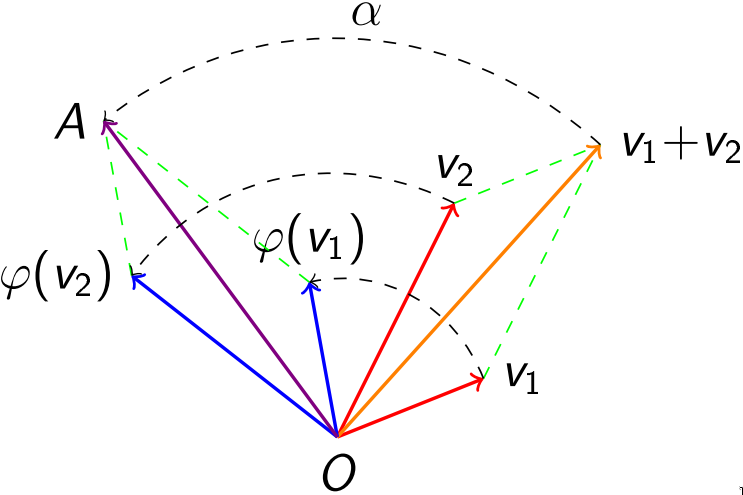
\includegraphics[height=5cm]{lecture16_example2_1}
    \hspace{2cm}
    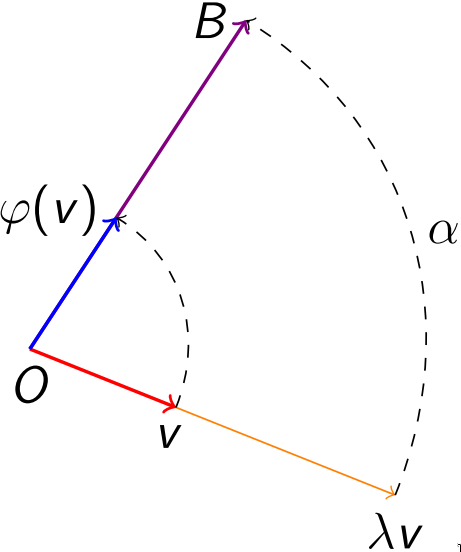
\includegraphics[height=5cm]{lecture16_example2_2}
\end{center}

\bigskip
\begin{enumerate}[label=\arabic*), nosep]
\item $\phi(v_1) + \phi(v_2) = A = \phi(v_1 + v_2)$,
\item $\phi(\lambda \cdot v) = B = \lambda \cdot \phi(v)$.
\end{enumerate}

\subsubsection{Пример 3}

$\phi\colon \RR^3 \to \RR^2$ --- ортогональная проекция на плоскость $Oxy$.

\begin{center}
    $\langle$ Конкурс на лучшую картинку $\rangle$
\end{center}

\subsubsection{Пример 4}

$\RR[x]_{\leq n}$ --- пространство многочленов от $x$ степени $\leq n$ с коэффициентами из $\RR$.

$\Delta \colon f(x) \mapsto f'(x)$ --- отображение дифференциирования.

\bigskip
\begin{enumerate}[label=\arabic*), nosep]
\item \label{lec16:example4_1} $(f + g)' = f' + g'$,
\item \label{lec16:example4_2} $(\lambda \cdot f)' = \lambda \cdot f' \quad \forall \lambda \in \RR$.
\end{enumerate}

\bigskip
\ref{lec16:example4_1} и \ref{lec16:example4_2} $\implies \Delta $ --- линейное отображение $\RR[x]_{\leq n} \to \RR[x]_{\leq n - 1}$.

\subsubsection{Пример 5}
\label{lec16:example_5}

$V$ --- векторное пространство над $F$, $\dim V = n$.

$(e_1, \dots, e_n)$ --- базис $V$.

$\phi \colon V \to F^n$

$v = x_1 e_1 + \dots + x_n e_n \implies \phi(v) := \begin{pmatrix} x_1 \\ \vdots \\ x_n \end{pmatrix}$.

Покажем, что оно линейно:

Пусть \begin{equation*}
    v = x_1 e_1 + \dots + x_n e_n \implies \phi(v) := \begin{pmatrix} x_1 \\ \vdots \\ x_n \end{pmatrix}
,\end{equation*} 
\begin{equation*}
    w = y_1 e_1 + \dots + y_n e_n \implies \phi(w) = \begin{pmatrix} y_1 \\ \vdots \\ y_n \end{pmatrix}
.\end{equation*}

Тогда,
\begin{enumerate}[label=\arabic*), nosep]
    \item \label{lec16:example5_1} $v + w = (x_1 + y_1) e_1 + \dots + (x_n + y_n) e_n \implies \phi(v + w) = \begin{pmatrix} x_1 + y_1 \\ \vdots \\ x_n + y_n \end{pmatrix} = \begin{pmatrix} x_1 \\ \vdots \\ x_n \end{pmatrix} + \begin{pmatrix} y_1 \\ \vdots \\ y_n \end{pmatrix} = \phi(v) + \phi(w)$,
    \item \label{lec16:example5_2} $\lambda \cdot v = (\lambda x_1) e_1 + \dots + (\lambda x_n) e_n \implies \phi(\lambda \cdot v) = \begin{pmatrix} \lambda x_1 \\ \vdots \\ \lambda x_n \end{pmatrix} = \lambda \begin{pmatrix} x_1 \\ \vdots \\ x_n \end{pmatrix} = \lambda \phi(v)$.
\end{enumerate}

\subsection{Простейшие свойства линейных отображений}

Здесь $\overrightarrow{0_V}$ --- нулевой вектор в векторном пространстве $V$.

\begin{enumerate}
\item $\phi(\overrightarrow{0_V}) = \overrightarrow{0_W}$.

    Доказательство: $\phi(\overrightarrow{0_V}) = \phi(0 \cdot \overrightarrow{0_V}) = 0 \cdot \phi(\overrightarrow{0_V}) = \phi(\overrightarrow{0_W})$.

\item $\phi(-v) = -\phi(v)$.

    Доказательство: $\phi(-v) + \phi(v) = \phi(-v + v) = \phi(0) = \phi(\overrightarrow{0_V)} = \overrightarrow{0_W} \implies \phi(-v) = -\phi(v)$.
\end{enumerate}


\subsection{Изоморфизм векторных пространств}

\begin{definition}
    Отображение $\phi \colon V \to W$ называется \textit{изоморфизмом} если оно линейно и биективно.

    Обозначение: $\phi \colon V \MapsTo W$.
\end{definition}

В примерах выше:
\begin{enumerate}[nosep]
\setcounter{enumi}{-1}
\item $\phi$ --- изоморфизм $\iff \begin{cases}
    V = \{\overrightarrow{0}\}, \\
    W = \{\overrightarrow{0}\}
\end{cases}$

\item да
\item да
\item нет
\item $\phi$ --- изоморфизм $\iff n = 0$
\item да!
\end{enumerate}


\subsection{Отображение, обратное к изоморфизму}

\begin{proposal}
    \label{lec16:prop_1}
    Если $\phi \colon V \to W$ --- изоморфизм, то $\phi^{-1}$ --- тоже изоморфизм. 
\end{proposal}

\begin{proof}
    Биективность есть, так как $\phi^{-1}$ --- обратное отображение.

    Проверим линейность
    \begin{enumerate}[label=\arabic*)]
    \item $w_1, w_2 \in W \implies w_1 = \phi(\phi^{-1}(w_1))$, $w_2 = \phi(\phi^{-1}(w_2))$
        \begin{align*}
            \phi^{-1}(w_1 + w_2) &= \phi^{-1}\Big(\underbrace{\phi\left(\phi^{-1}(w_1)\right)}_{w_1} + \underbrace{\phi\left(\phi^{-1}(w_2)\right)}_{w_2}\Big) \\
            &= \underbrace{\phi^{-1}\big(\phi}_{Id}\left(\phi^{-1}(w_1) + \phi^{-1}(w_2)\right)\!\big)\\
            &= \phi^{-1}(w_1) + \phi^{-1}(w_2)
        .\end{align*}

    \item 
        \begin{align*}
            \phi^{-1}(\lambda \cdot w_1) &= \phi^{-1}\left(\lambda \cdot \phi\left(\phi^{-1}\left(w_1\right)\right)\right) \\
            &= \underbrace{\phi^{-1}\big(\phi}_{Id}\left(\lambda \cdot \phi^{-1}(w_1)\right)\!\big) \\
            &= \lambda \phi^{-1}(w_1)
        .\qedhere\end{align*}
    \end{enumerate}
\end{proof}


\subsection{Композиция двух линейных отображений, композиция двух изоморфизмов}

Пусть $U \xrightarrow{\psi} V \xrightarrow{\phi} W$, тогда $\phi \circ \psi : U \to W$ --- композиция.

\begin{proposal}~
    \label{lec16:prop_2}
    \begin{enumerate}[nosep]
    \item Если $\phi$, $\psi$ линейны, то $\phi \circ \psi$ тоже линейна.
    \item Если $\phi$, $\psi$ --- изоморфизмы, то $\phi \circ \psi$ --- тоже изоморфизм.
    \end{enumerate}
\end{proposal}

\begin{proof}~
    \begin{enumerate}
    \item \label{lec16:comp_1}
        \begin{enumerate}[label=(\arabic*)]
            \item $(\phi \circ \psi)(u_1 + u_2) = \phi(\psi(u_1 + u_2)) = \phi(\psi(u_1) + \psi(u_2)) = \phi(\psi(u_1)) + \phi(\psi(u_2)) = (\phi \circ \psi)(u_1) + (\phi \circ \psi)(u_2)$.
            \item $(\phi \circ \psi)(\phi u) = \phi(\psi(\lambda u)) = \phi(\lambda \psi(u)) = \lambda \phi(\psi(u)) = \lambda(\phi \circ \psi)(u)$.
        \end{enumerate}
    \item из \ref{lec16:comp_1} следует, что $(\phi \circ \psi)$ линейно, но при этом биективно как композиция двух биекций.
        \qedhere
    \end{enumerate}
\end{proof}


\subsection{Изоморфные векторные пространства}

\begin{definition}
    Два векторных пространства $V$, $W$ называются \textit{изоморфными}, если существует изоморфизм \\ ${\phi\colon V \MapsTo W}$.

    Обозначается: $V \simeq W$ (либо $V \cong W$).
\end{definition}


\subsection{Отношение изоморфности на множестве всех векторных пространств}

\begin{theorem}
    Отношение изоморфности является отношением эквивалентности на множестве всех векторных пространств над фиксированным полем $F$.
\end{theorem}

\begin{proof}~
    \begin{enumerate}
    \item Рефлексивность: $Id: V \MapsTo V$.
    \item Симметричность: $V \simeq W \implies W \simeq V$ следует из \hyperref[lec16:prop_1]{Предложения 1}.
    \item Транзитивность: $U \simeq V$, $V \simeq W \implies U \simeq W$ следует из \hyperref[lec16:prop_2]{Предложения 2}.
        \qedhere
    \end{enumerate}
\end{proof}


\subsection{Классы изоморфизма векторных пространств}

\begin{definition}
    Классы эквивалентности называются \textit{классами изоморфизма}.   
\end{definition}

\begin{example}
    $F[x]_{\leq n} \simeq F^{n + 1}$:

    $a_0 + a_1 x + \dots + a_n x^n \longleftrightarrow \begin{pmatrix} a_0 \\ a_1 \\ \vdots \\ a_n \end{pmatrix}$.
\end{example}


\subsection{Критерий изоморфности двух конечномерных векторных пространств}

\begin{theorem}
    Пусть $V$, $W$ --- два конечномерных векторных пространства над $F$.

    Тогда, $V \simeq W \iff \dim V = \dim W$.
\end{theorem}

\begin{lemma}
    \label{lec16:lemma_1}
    $\dim V = n \implies V \simeq F^n$.
\end{lemma}

\begin{proof}
    Фиксируем базис $(e_1, \dots, e_n)$ в $V$.

    Тогда, отображение $\phi \colon V \to F^n$ из \hyperref[lec16:example_5]{Примера 5} --- изоморфизм.
\end{proof}

\begin{lemma}
    \label{lec16:lemma_2}
    Пусть $\phi \colon V \MapsTo W$ и $e_1, \dots, e_n$ --- базис $V$, тогда $\phi(e_1), \dots, \phi(e_n)$ --- базис $W$. 
\end{lemma}

\begin{proof}
    Пусть $w \in W$. Тогда $\exists x_1, \dots, x_n \in F$, такие что $\phi^{-1}(w) = x_1 e_1 + \dots + x_n e_n$.

    Тогда, $w = \phi\left(\phi^{-1}(w)\right) = \phi(x_1 e_1 + \dots + x_n e_n) = x_1 \phi(e_1) + \dots + x_n \phi(e_n) \implies W = \langle \phi(e_1), \dots, \phi(e_n) \rangle$.

    Теперь докажем линейную независимость:

    Пусть $\alpha_1 \phi(e_1) + \dots + \alpha_n \phi(e_n) = \overrightarrow{0}$.

    Тогда, $\phi(\alpha_1 e_1 + \dots + \alpha_n e_n) = \overrightarrow{0}$.

    Применяя $\phi^{-1}$ получаем, $\alpha_1 e_1 + \dots + \alpha_n e_n = \phi^{-1}(\overrightarrow{0}) = \overrightarrow{0}$. Значит, $\alpha_1 = \dots = \alpha_n = 0$.

    Итог: $\phi(e_1), \dots, \phi(e_n)$ --- базис в $V$.
\end{proof}

\begin{proof}[Доказательство теоремы]~
    \begin{description}
    \item[$\impliedby$] Пусть $\dim V= \dim W = n$. Тогда по \hyperref[lec16:lemma_1]{лемме 1} $V \simeq F^n, W \simeq F^n$, значит $V \simeq W$.
    \item[$\implies$] Пусть $V \simeq W$. Фиксируем изоморфизм $\phi \colon V \MapsTo W$.

        Тогда по \hyperref[lec16:lemma_2]{лемме 2} получаем, что $\phi(e_1), \dots, \phi(e_n)$ --- базис $W$, а значит $\dim V = n = \dim W$.
        \qedhere
    \end{description}
\end{proof}

\begin{exercise}
    Если $\dim V = n$, то все изоморфизмы $V \MapsTo F^n$ находятся в биекции с базисами пространства $V$.
\end{exercise}


\subsection{Задание линейного отображения путём задания образов векторов фиксированного базиса}

Пусть $V$, $W$ --- векторные пространства над $F$ и $(e_1, \dots, e_n)$ --- фиксированный базис в $V$.

\begin{proposal}~
    \label{lec16:propopop}
    \begin{enumerate}
    \item Если $\phi \colon V \to W$ --- линейное отображение, то $\phi$ однозначно определяется векторами $\phi(e_1), \dots, \phi(e_n)$,
    \item $\forall w_1, \dots, w_n \in W \ \exists!$ линейное отображение $\phi$, такое что, $\phi(e_1) = w_1, \dots, \phi(e_n) = w_n$.
    \end{enumerate}
\end{proposal}

\begin{proof}~
    \begin{enumerate}
    \item \label{lec16:kekek}
        $v \in V \implies v = x_1 e_1 + \dots + x_n e_n \implies \phi(v) = x_1 \phi(e_1) + \dots + x_n \phi(e_n)$.
    \item 
        Зададим $\phi \colon V \to W$ формулой $\phi(x_1 e_1 + \dots + x_n e_n) = x_1 w_1 + \dots + x_n w_n$.

        Тогда $\phi$ --- линейное отображение из $V$ в $W$ (упражнение).

        Единственность следует из \ref{lec16:kekek}
        \qedhere
    \end{enumerate}
\end{proof}

    \section{Лекция 23.01.2020}

\newcommand\E{\mathbbm{e}}
\newcommand\F{\mathbbm{f}}
\let\G\undefined
\newcommand\G{\mathbbm{g}}


\subsection{Матрица линейного отображения}

Пусть $V, W$ --- векторные пространства над $F$.

$\E = (e_1, \dots, e_n)$ --- базис $V$,

$\F = (f_1, \dots, f_m)$ --- базис $W$.

\bigskip
Пусть $\phi: V \to W$ --- линейное отображение.

$\forall j = 1, \dots, n$

$\phi(e_j) = a_{1j} f_1 + a_{2j} f_2 + \dots + a_{mn} f_m = (f_1, \dots, f_m) \begin{pmatrix} a_{1j} \\ a_{2j} \\ \dots \\ a_{mj} \end{pmatrix}$.

Тогда, $(\phi(e_1), \dots, \phi(e_n)) = (f_1, \dots, f_n) \cdot A$, где $A = (a_{ij}) \in \text{Mat}_{m \times n} (F)$.

\begin{definition}
    $A$ называется матрицей линейного отображения $\phi$ в базисах $\E$ и $\F$.

    Обозначение: $A = A(\phi, \E, \F)$.
\end{definition}

В $j$-м столбце матрицы $A$ стоят координаты вектора $\phi(e_j)$ в базисе $\F$.

\begin{designation}
    $\hom(V, W) := $ множество всех линейных отображений из $V$ в $W$.
\end{designation}

\begin{corollary}[из предложения \ref{lec16:propopop}]
    При фиксированных базисах $\E$ и $\F$ отображение $\phi \mapsto A(\phi, \E, \F)$ является биекцией между $\hom(V, W)$ и $\text{Mat}_{m \times n}(F)$.
\end{corollary}


\subsection{Примеры}

\begin{enumerate}[start=0]
\item $\phi(v) = 0 \ \forall v \implies \forall \E, \F \ A(\phi, \E, \F) = \begin{pmatrix} 0 & \dots & 0 \\ \vdots & \ddots & \vdots \\ 0 & \dots & 0 \end{pmatrix}$.
\stepcounter{enumi}
\stepcounter{enumi}
\item $\RR^3 \to \RR^2$ --- проекция на $Oxy$.

    \begin{math}
        \left.
            \begin{aligned}
                \E \text{ --- стандартный базис в } \RR^3 \\
                \F \text{ --- стандартный базис в } \RR^2
            \end{aligned}
        \right\} \implies A(\phi, \E, \F) = \begin{pmatrix} 
            1 & 0 & 0 \\
            0 & 1 & 0
        \end{pmatrix}.
    \end{math}

\item $\Delta : \RR[x]_{\leq n} \to \RR[x]_{\leq n - 1}$, $f \to f'$.

    $\E = (1, x, \dots, x^n)$, $\F = (1, x, \dots, x^{n - 1})$.

    \begin{math}
        A(\phi, \E, \F) = \begin{pmatrix} 
            0 & 1 & 0 & 0 & \dots & 0 \\
            0 & 0 & 2 & 0 & \dots & 0 \\
            0 & 0 & 0 & 3 & \dots & 0 \\
            \vdots & \vdots & \vdots & \vdots & \ddots & \vdots \\
            0 & 0 & 0 & 0 & \dots & n
        \end{pmatrix}
    \end{math}

\item $x_1 e_1 + \dots + x_n e_n \mapsto \begin{pmatrix} x_1 \\ \dots \\ x_n \end{pmatrix}$.

    \begin{math}
        \left.
        \begin{aligned}
            \E &= (e_1, \dots, e_n) \\
            \F &= \text{стандартный базис}
        \end{aligned}
        \right\} \implies A(\phi, \E, \F) = E.
    \end{math}

\item $\phi: F^n \to F^m$.

    $\phi(x) = A \cdot x$, $A \in \text{Mat}_{m \times n}(F)$.

    $\E = $ стандартный базис,

    $\F = $ стандартный базис.

    $A(\phi, \E, \F) = A$.
\end{enumerate}


\subsection{Связь координат вектора и его образа при линейном отображении}

\begin{proposal}
    Пусть $\phi : V \to W$ --- линейное отображение,

    $\E = (e_1, \dots, e_n)$ --- базис $V$,

    $\F = (f_1, \dots, f_m)$ --- базис $W$,

    $A = A(\phi, \E, \F)$.

    \begin{math}
        \begin{aligned}
            v \in V \implies &v = x_1 e_1 + \dots + x_n e_n, \\
            &\phi(v) = y_1 f_1 + \dots + y_m f_m.
        \end{aligned}
    \end{math}

    Тогда,
    \begin{equation*}
        \begin{pmatrix} y_1 \\ \vdots \\ y_m \end{pmatrix} = A \begin{pmatrix} x_1 \\ \vdots \\ x_n \end{pmatrix}
    .\end{equation*}
\end{proposal}

\begin{proof}
    $v = (e_1, \dots, e_m) \begin{pmatrix} x_1 \\ \vdots \\ x_n \end{pmatrix}$.

    Значит, 
    \begin{align*}
        \phi(v) &= (\phi(e_1), \dots, \phi(e_n)) \begin{pmatrix} x_1 \\ \vdots \\ x_n \end{pmatrix} = (f_1, \dots, f_m) \cdot A \cdot \begin{pmatrix} x_1 \\ \vdots \\ x_n \end{pmatrix}
    .\end{align*}

    При этом, 
    \begin{align*}
        \phi(v) = (f_1, \dots, f_m) \begin{pmatrix} y_1 \\ \vdots \\ y_m \end{pmatrix}
    .\end{align*}

    Так как $f_1, \dots, f_m$ линейно независимы, то
    \begin{equation*}
        A \begin{pmatrix} x_1 \\ \vdots \\ x_n \end{pmatrix} = \begin{pmatrix} y_1 \\ \vdots \\ y_m \end{pmatrix}
    .\end{equation*}
\end{proof}


\subsection{Формула изменения матрицы линейного отображения между векторными пространствами $V$ и $W$ при замене их базисов}

Пусть теперь $\E'$ --- другой базис в $V$, $\F'$ --- другой базис в $W$.

$\E' = \E \cdot C_{\in M_n}$,

$\F' = \F \cdot D_{\in M_m}$.

$A = A(\phi, \E, \F)$,

$A' = A(\phi, \E', \F')$.

\begin{proposal}
    $A' = D^{-1} A C$.
\end{proposal}

\begin{proof}
    \begin{equation*}
        (e'_1, \dots e'_n) = (e_1, \dots, e_n) \cdot C
    .\end{equation*}
    Применим $\phi$, 
    \begin{align*}
        (\phi(e'_1), \dots, \phi(e'_n)) &= (\phi(e_1), \dots, \phi(e_n)) \cdot C = (f_1, \dots, f_m) \cdot A \cdot C
    \end{align*}
    При этом,
    \begin{align*}
        (\phi(e'_1), \dots, \phi(e'_n)) &= (f'_1, \dots, f'_m) \cdot A' = (f_1, \dots, f_m) \cdot D \cdot A'
    .\end{align*}

    Отсюда,
    \begin{equation*}
        A \cdot C = D \cdot A' \implies A' = D^{-1} \cdot A \cdot C
    .\qedhere\end{equation*}
\end{proof}


\subsection{Операции сложения и умножения на скаляр на множестве всех линейных отображений между двумя векторными пространствами}

Пусть $\phi, \psi \in \hom(V, W)$, $\lambda \in F$.

\begin{definition}~
    \begin{enumerate}
    \item \textit{Суммой} линейных отображений $\phi$ и $\psi$ называется линейное отображение $\phi + \psi \in \hom(V, W)$, \\ такое что ${(\phi + \psi)(v) := \phi(v) + \psi(v)}$.
    \item Произведение $\phi$ на $\lambda$ --- это линейное отображение $\lambda \phi \in \hom(V, W)$, такое что $(\lambda\phi)(v) := \lambda \phi(v)$.
    \end{enumerate}
\end{definition}

\begin{exercise}
    $\phi + \psi$ и $\lambda \phi$ --- действительно линейные отображения.
\end{exercise}

\begin{exercise}
    $\hom(V, W)$ с этими операциями является векторным пространством над $F$.
\end{exercise}


\subsection{Матрица суммы двух линейных отображений и произведения линейного отображения на скаляр}

Зафиксируем базисы $\E = (e_1, \dots, e_n)$ в $V$ и $\F = (f_1, \dots, f_m)$ в $W$.

\begin{proposal}~
    \begin{enumerate}
    \item
        \begin{math}
            \begin{aligned}[t]
                \phi, \psi \in \hom(V, W), \
                &A_\phi = A(\phi, \E, \F)& \\
                &A_\psi = A(\psi, \E, \F)& \\
                &A_{\phi + \psi} = A(\phi + \phi, \E, \F)& \implies A_{\phi + \psi} = A_\phi + A_\psi
            \end{aligned}
        \end{math}

    \item
        \begin{math}
            \begin{aligned}[t]
                \lambda \in F, \phi \in \hom(V, W), \
                &A_\phi = A(\phi, \E, \F)& \\
                &A_{\lambda \phi} = A(\lambda \phi, \E, \F)& \implies A_{\lambda \phi} = \lambda A_\phi
            \end{aligned}
        \end{math}
    \end{enumerate}
\end{proposal}

\begin{proof}~
    \begin{enumerate}
    \item 
        \begin{align*}
            (f_1, \dots, f_m) \cdot A_{\phi + \psi}
            &= ((\phi + \psi)(e_1), \dots, (\phi + \psi)(e_n)) \\
            &= (\phi(e_1), \dots, \phi(e_n)) + (\psi(e_1), \dots, \psi(e_n)) \\
            &= (f_1, \dots, f_m) A_\phi + (f_1, \dots, f_m) A_\psi \\
            &= (f_1, \dots, f_m) (A_\phi + A_\psi)
        .\end{align*}

        Следовательно, $A_{\phi + \psi} = A_\phi + A_\psi$.

    \item Аналогично. \qedhere
    \end{enumerate}
\end{proof}


\subsection{Изоморфизм между пространством $\hom(V,W)$ и пространством $(m \times n)$-матриц, где $n = \dim V$, $m = \dim W$}

\begin{corollary}
    При фиксированном $\E$ и $\F$ отображение $\phi \mapsto A(\phi, \E, \F)$ является изоморфизмом между $\hom(V, W)$ и $\text{Mat}_{m \times n}(F)$.
\end{corollary}

\begin{proof}~
    Биективность была выше.
    Линейность --- из предыдущего предложения.
\end{proof}

\begin{corollary}
    $\dim \hom(V, W) = m \cdot n$.
\end{corollary}


\subsection{Матрица композиции двух линейных отображений}

Пусть $U \xrightarrow{\psi} V \xrightarrow{\phi} W$ --- цепочка линейных отображений, а $\phi \circ \psi : U \to W$ --- их композиция,

$\E = (e_1, \dots, e_n)$ --- базис $V$,

$\F = (f_1, \dots, f_m)$ --- базис $W$,

$\G = (g_1, \dots, g_k)$ --- базис $U$.

$A_{\phi} = A(\phi, \E, \F)$,

$A_\psi = A(\psi, \G, \E)$,

$A_{\phi \circ \psi} = A(\phi \circ \psi, \G, \F)$.

Тогда, $A_{\phi \circ \psi} = A_\phi \cdot A_\psi$.

\begin{proof}
    $(\psi(g_1), \dots, \psi(g_k)) = (e_1, \dots, e_n) A_\psi$.
    Тогда применяя $\phi$,
    \begin{equation*}
        \left(\phi\left(\psi(g_1)\right), \dots, \phi\left(\psi(g_k)\right)\right) = \left(\phi(e_1), \dots, \phi(e_n)\right) A_\psi = (f_1, \dots, f_m) A_\phi A_\psi
    .\end{equation*}
    С другой стороны,
    \begin{equation*}
        \left(\phi\left(\psi(g_1)\right), \dots, \phi\left(\psi(g_k)\right)\right) = (f_1, \dots, f_m) A_{\phi \circ \psi}
    .\end{equation*}

    Значит, $A_\phi \cdot A_\psi = A_{\phi \circ \psi}$.
\end{proof}


\subsection{Ядро и образ линейного отображения; утверждение о том, что они являются подпространствами в соответствующих векторных пространствах}

Пусть $\phi : V \to W$.

\begin{definition}
    \textit{Ядро} линейной оболочки $\phi$ --- это $\ker \phi := \{v \in V \mid \phi(v) = 0\} \subseteq V$.

    \textit{Образ} линейного отображения $\phi$ --- это $\Im \phi := \phi(V) \subseteq W$.
\end{definition}

\begin{example}
    $\Delta : \RR[x]_{\leq n} \to \RR[x]_{\leq n}, \ f \mapsto f'$,

    $\ker \Delta = \{f \mid f = \text{const}\}$,

    $\Im \Delta = \RR[x]_{\leq n - 1}$.
\end{example}

\begin{proposal}~
    \begin{enumerate}
    \item Ядро --- подпространство в $V$.
    \item Образ --- подпространство в $W$.
    \end{enumerate}
\end{proposal}

\begin{proof}~
    \begin{enumerate}
    \item 
        \begin{enumerate}
        \item $\phi(0_V) = 0_W$,
        \item $v_1, v_2 \in \ker \phi \implies \phi(v_1 + v_2) = \phi(v_1) + \phi(v_2) = 0 + 0 = 0 \implies v_1 + v_2 \in \ker \phi$,
        \item $\lambda \in F, v \in V \implies \phi(\lambda v) = \lambda \phi(v) = \lambda 0 = 0 \implies \lambda v \in \ker \phi$.
        \end{enumerate}

    \item
        \begin{enumerate}
        \item $0_W = \phi(W) \in \Im \phi$,
        \item $w_1, w_2 \in \Im \phi \implies \exists v_1, v_2 : w_1 = \phi(v_1), w_2 = \phi(v_2) \implies w_1 + w_2 = \phi(v_1) + \phi(v_2) = \phi(v_1 + v_2) \in \Im \phi$,
        \item $\phi \in F, w \in \Im \phi \implies \exists v \in V : w = \phi(v) \implies \phi(w) = \lambda \phi(v) = \phi(\lambda v) \in \Im \phi$.
            \qedhere
        \end{enumerate}
    \end{enumerate}
\end{proof}

    \section{Лекция 25.01.2020}

\subsection{Критерий инъективности линейного отображения в терминах его ядра}

Пусть $V, W$ --- векторные пространства над $F$, 

$\phi \colon V \to W$ --- линейное отображение.

Ядро: $\ker \phi := \{v \in V \mid \phi(v) = 0\} \subseteq V$.

Образ: $\Im \phi := \phi(V) \subseteq W$.

\begin{proposal}~
    \begin{enumerate}[label=(\alph*)]
    \item $\phi$ инъективно $\iff \ker \phi = \{0\}$,
    \item $\phi$ сюръективно $\iff \Im \phi = W$.
    \end{enumerate}
\end{proposal}

\begin{proof}~
    \begin{enumerate}[label=(\alph*)]
    \item 
        \begin{description}[leftmargin=0.935cm]
        \item[$\implies$] очевидно
        \item[$\impliedby$] 
            Пусть $v_1, v_2 \in V$ таковы, что $\phi(v_1) = \phi(v_2)$. 
            Тогда $\phi(v_1 - v_2) = 0$, а значит $v_1 - v_2 \in \ker \phi$.

            Но тогда, $v_1 - v_2 = 0$, то есть $v_1 = v_2$.
        \end{description}
    \item очевидно.
        \qedhere
    \end{enumerate}
\end{proof}

\begin{corollary}
    $\phi$ изоморфизм
    \begin{math}
        \iff
        \left\{
        \begin{aligned}
            \ker \phi &= \{0\},\\
            \Im \phi &= W.
        \end{aligned}
        \right.
    \end{math}
\end{corollary}


\subsection{Характеризация изоморфизмов в терминах их ядер и образов}

Пусть $U \subseteq V$ --- подпространство, $u_1, \dots, u_k$ --- базис в $U$.

\begin{lemma}
    Тогда, $\phi(U) = \left< \phi(u_1), \dots, \phi(u_k) \right>$.
    В частности, $\dim \phi(U) \leq \dim U$ и $\dim \Im \phi \leq \dim V$.
\end{lemma}

\begin{proof}
    $u \in U \implies u = \alpha_1 u_1 + \dots + \alpha_k u_k$, $\alpha_i \in F$, тогда
    \begin{equation*}
        \phi(u) = \alpha_1 \phi(u_1) + \dots + \alpha_k \phi(u_k) \in \left< \phi(u_1), \dots, \phi(u_k) \right>
    .\qedhere\end{equation*}
\end{proof}


\subsection{Связь размерности образа линейного отображения с рангом его матрицы}

Пусть 
\begin{math}
    \begin{aligned}[t]
        \E &= (e_1, \dots, e_n) \text{ --- базис $V$}, \\
        \F &= (f_1, \dots, f_m) \text{ --- базис $W$}, \\
        A &= A(\phi, \E, \F).
    \end{aligned}
\end{math}

\begin{theorem}
    $\rk A = \dim \Im \phi$.
\end{theorem}

\begin{proof}
    По лемме, $\Im \phi = \left< \phi(e_1), \dots, \phi(e_n) \right>$. Поэтому, $\dim \Im \phi = \rk \{\phi(e_1), \dots, \phi(e_n)\}$.

    Так как $j$-й столбец матрицы $A$ составлен из координат вектора $\phi(e_j)$ в базисе $\F$, то
    \begin{equation*}
        \alpha_1 \phi(e_1) + \dots + \alpha_n \phi(e_n) = 0 \iff \alpha_1 A^{(1)} + \dots + \alpha_n A^{(n)} = 0
    .\end{equation*}

    Значит, $\dim \Im \phi = \rk \{\phi(e_1), \dots, \phi(e_n)\} = \rk \{A^{(1)}, \dots, A^{(n)}\} = \rk A$.
\end{proof}

\begin{comment}
    Число $\dim \Im \phi$ называется \textit{рангом} линейного отображения $\phi$, обозначается $\rk \phi$.
\end{comment}

\begin{corollary}
    $\rk A$ не зависит от выбора пары базисов $\E$ и $\F$.
\end{corollary}


\subsection{Инвариантность ранга матрицы относительно умножения на квадратную невырожденную матрицу слева или справа}

\begin{designation}
    $M^{0}_n(F) := \{ C \in M_n(F) \mid \det C \neq 0\}$.  
\end{designation}

\begin{corollary}
    Ранг матрицы не меняется при умножении слева и/или справа на невырожденную матрицу.
\end{corollary}

\begin{proof}
    Если $A \in \text{Mat}_{m \times n}$, $C \in M^{0}_n$, $D \in M_m^{0}$, то $A$ и $D^{-1}AC$ --- это матрицы одного и того же линейного отображения в разных парах базисов.
    По теореме, $\rk A = \rk\left(D^{-1}AC\right)$.
\end{proof}


\subsection{Свойство образов векторов, дополняющих базис ядра до базиса всего пространства}

\begin{proposal}
    Пусть $e_1, \dots, e_k$ --- базис $\ker \phi$ и векторы $e_{k + 1}, \dots, e_n$ дополняют его до базиса всего $V$.

    Тогда, $\phi(e_{k + 1}), \dots, \phi(e_n)$ образуют базис в $\Im \phi$.
\end{proposal}

\begin{proof}
    $\Im \phi = \left< \phi(e_1), \dots, \phi(e_k), \phi(e_{k + 1}), \dots, \phi(e_n) \right> = \left< \phi(e_{k + 1}), \dots, \phi(e_n) \right>$. (так как $\phi(e_1) = \dots = \phi(e_k) = 0$).

    Осталось показать, что $\phi(e_{k + 1}), \dots, \phi(e_n)$ линейно независимы.

    Пусть $\alpha_{k + 1} \phi(e_{k + 1}) + \dots + \alpha_n \phi(e_n) = 0$, где $\alpha_i \in F$.

    Тогда $\phi(\alpha_{k + 1} e_{k + 1} + \dots \alpha_n e_n) = 0 \implies \alpha_{k + 1} e_{k + 1} + \dots + \alpha_n e_n \in \ker \phi$.

    Но тогда $\alpha_{k + 1} e_{k + 1} + \dots \alpha_n e_n = \beta_1 e_1 + \dots + \beta_k e_k$, где $\beta_j \in F$.

    Так как $(e_1, \dots, e_n)$ --- базис $V$, то $\alpha_i = \beta_j = 0 \ \forall i, j$.
\end{proof}


\subsection{Теорема о связи размерностей ядра и образа линейного отображения}

\begin{theorem}
    $\dim \Im \phi + \dim \ker \phi = \dim V$.
\end{theorem}

\begin{proof}
    Вытекает из предыдущего предложения так как в его доказательстве:

    $\dim V = n$,

    $\dim \ker \phi = k$,

    $\dim \Im \phi = n - k$.
\end{proof}


\subsection{Приведение матрицы линейного отображения к диагональному виду с единицами и нулями на диагонали}

\begin{proposal}
    Пусть $\rk \phi = r$. Тогда существует базис $\E$ в $V$ и базис $\F$ в $W$, такие что
    \begin{equation*}
        A(\phi, \E, \F) = \left(
            \begin{array}{c|c}
                E & 0 \\
                \hline
                0 & 0
            \end{array}
        \right) = \bordermatrix{    
            &   & r &   &   &   & n - r &   \cr
            & 1 & 0 & 0 & \dots & 0 & 0 & 0 \cr
          \hspace{0.7cm} r & 0 & \ddots & 0 & \dots & 0 & 0 & 0 \cr
            & 0 & 0 & 1 & \dots & 0 & 0 & 0 \cr
            & \vdots & \vdots & \vdots & \ddots & \vdots & \vdots & \vdots \cr
            & 0 & 0 & 0 & \dots & 0 & 0 & 0 \cr
      m - r & 0 & 0 & 0 & \dots & 0 & 0 & 0 \cr
            & 0 & 0 & 0 & \dots & 0 & 0 & 0
        }
    .\end{equation*}
\end{proposal}

\begin{proof}
    Пусть $e_{r + 1}, \dots, e_n$ --- базис $\ker \phi$. Дополним его векторами $e_1, \dots, e_r$ до базиса всего $V$.

    Положим $f_1 = \phi(e_1)$, $\dots$, $f_r = \phi(e_r)$, тогда $(f_1, \dots, f_r)$ --- базис $\Im \phi$.

    Дополним $f_1, \dots, f_r$ до базиса $f_1, \dots, f_m$ всего $W$.

    Тогда, $\E = (e_1, \dots, e_n)$ и $\F = (f_1, \dots, f_m)$ --- искомые базисы.
\end{proof}

\begin{corollary}
    Если $A \in \text{Mat}_{m \times n}(F)$, $\rk A = r$, то $\exists C \in M_n^{0}(F)$ и $D \in M_m^{0}(F)$, такие что
    \begin{equation*}
        D^{-1}AC = \left(
            \begin{array}{c|c}
                E & 0 \\
                \hline
                0 & 0
            \end{array}
        \right) = B
    .\end{equation*}

    $(\iff A = DBC^{-1})$.
\end{corollary}

\begin{proof}
    Реализуем $A$ как матрицу линейного отображения $\phi \colon F^{n} \to F^m$ в некоторой паре базисов, тогда утверждение вытекает из предложения и формулы изменения матрицы линейного отображения при замене базисов.
\end{proof}


\subsection{Линейные функции на векторном пространстве}

\begin{definition}
    \textit{Линейной функцией} (или \textit{линейной формой}, или \textit{линейным функционалом}) на $V$ называется всякое линейное отображение $\alpha \colon V \to F$.
\end{definition}

\begin{designation}
    $V^{*} := \hom(V, F)$ --- множество всех линейных функций на $V$.
\end{designation}


\subsection{Примеры}

\begin{enumerate}
\item $\alpha \colon F^n \to F$.

    $\alpha \begin{pmatrix} x_1 \\ \dots \\ x_n \end{pmatrix} = (a_1, \dots, a_n) \begin{pmatrix} x_1 \\ \dots \\ x_n \end{pmatrix} = a_1 x_1 + \dots + a_n x_n$, где $a_i \in F$ --- фиксированные скаляры.

\item $F(X, \RR)$ --- все функции из линейного пространства $X$ в $\RR$, $x_0 \in X$,

    $\alpha \colon F(X, \RR) \to \RR$,

    $\alpha(f) := f(x_0)$.

\item $\alpha \colon C[0, 1] \to \RR$

    $\alpha(f) := \displaystyle\int_0^1 f(x) \mathop{}\!d x$

\item $\alpha \colon M_n(F) \to F$

    $\alpha(X) := \tr X$
\end{enumerate}

\subsection{Двойственное (сопряжённое) векторное пространство, его размерность в конечномерном случае}

Из общей теории линейных отображений:
\begin{enumerate}
\item $V^{*}$ --- векторное пространство (оно называется \textit{сопряженным} или \textit{двойственным}).
\item Если $\E = (e_1, \dots, e_n)$ --- фиксированный базис в $V$, то есть изоморфизм $V^{*} \simeq \text{Mat}_{1 \times n}(F)$ (а это ни что иное, как строки длины $n$).

    $\alpha \to (\alpha_1, \dots, \alpha_n)$

    $v = x_1 e_1 + \dots + x_n e_n$

    $\alpha(v) = (\alpha_1, \dots, \alpha_n) \begin{pmatrix} x_1 \\ \dots \\ x_n \end{pmatrix} = \alpha_1 x_1 + \dots + \alpha_n x_n$.

    $\alpha_i = \alpha(e_i)$ --- коэффициенты линейной функции $\alpha$ в базисе $\E$.
\end{enumerate}

\begin{corollary}
    $\dim V^{*} = \dim V$ ($\implies V^{*} \simeq V$).
\end{corollary}


\subsection{Двойственный базис}

При $i = 1, \dots, n$ рассмотрим линейную функцию $\epsilon_i \in V^{*}$, соответствующую строке $(0 \dots 1 \dots 0)$. Тогда $\epsilon_1, \dots, \epsilon_n$ --- базис $V^{*}$, он однозначно определяется условием $\epsilon_i(e_j) = \delta_{ij} = \begin{cases}
    1, &i = j, \\
    0, &i \neq j.
\end{cases}$. ($\delta_{ij}$ --- символ Кронекера)


\begin{definition}
    Базис $(\epsilon_1, \dots, \epsilon_n)$ пространства $V^{*}$, определенный условием выше, называется базисом, \textit{двойственным} (сопряженным) к базису $\E$.

    Удобная запись условия:
    \begin{equation*}
        \begin{pmatrix} \epsilon_1 \\ \dots \\ \epsilon_n \end{pmatrix} (e_1, \dots, e_n) = E
    .\end{equation*}
\end{definition}

    \section{Лекция 8.02.2018}

$V$ -- векторное пространство

\textbf{Определение.} Линейной функцией (линейной формой, линейным функционалом) на $V$ называется всякое линейное отображение $\alpha : V \rightarrow F$.

Обозначение:$V^{*} := Hom(V, F)$ -- множество всех линейных функций на $V$

\vspace{\baselineskip}
Примеры:

1) $\alpha : F^n \rightarrow F, \begin{pmatrix} x_1 \\ \vdots \\ x_n \end{pmatrix} \rightarrow \alpha_1 x_1 + \dots + \alpha_n x_n$, где $\alpha_1, \dots, \alpha_n \in F$ -- фиксированные скаляры

2) $F(X, \RR)$ -- векторное пространство всех функций из множества $X$ в $\RR, x_0 \in X \Rightarrow \alpha : F(X, \RR) \rightarrow \RR, f \rightarrow f(x_0)$

3) $\alpha : C[a, b]$(непрерывные функции на $[a, b]$) $\rightarrow \RR, f \rightarrow \int^b_a f(x) dx$ 

4) $\alpha: M_n(F) \rightarrow F, A \rightarrow trA$

\vspace{\baselineskip}
Далее считаем, что $dimV = n < \infty$

Из общей теории линейных отображений:

1)$V^{*}$ -- векторное пространство (оно называется пространством, \textit{двойственным или сопряженным пространству} $V$)

2) Если $e = (e_1, \dots, e_n)$ -- фиксированный базис $V$, то имеется изоморфизм $V^{*} \iso Mat_{1 \times n}(F), \alpha \rightarrow (\alpha_1, \dots, \alpha_n)$, где $\alpha_i = \alpha(e_i)$ -- значение $\alpha$ на $e_i$ (коэффициенты линейной функции $\alpha$ в базисе $e$)

Если $x = x_1 e_1 + \dots + x_n e_n$, то $\alpha(x) = (\alpha_1, \dots, \alpha_n) \begin{pmatrix} x_1 \\ \vdots \\ x_n \end{pmatrix}$

\textbf{Следствие.} $dimV^* = dimV (\Rightarrow V^{*} \simeq V)$

\vspace{\baselineskip}
Фиксируем базис $e = (e_1, \dots, e_n)$ в $V$

$\forall i = 1, \dots, n$ рассмотрим линейную функцию $\varepsilon_i \in V^*$, такую что $\varepsilon_i(e_j) = \delta_{ij}$ (символ Кронекера) $\delta_{ij} = \begin{cases}
		1, i=j \\
		0, i \neq j
	\end{cases}$

\vspace{\baselineskip}
Соответствующая строка в $Mat_{1 \times n}(F)$ есть $
\bordermatrix{ 
& & & & i & & & &  \cr 
& 0 & \dots & 0 & 1 & 0 & \dots & 0} $

\vspace{\baselineskip}
Линейные функции $\varepsilon_i, i = 1, \dots, n$ образуют базис в $V^*$

\vspace{\baselineskip}
\textbf{Определение.} Базис $(\varepsilon_1, \dots, \varepsilon_n)$ пространства $V*$ называется \textit{двойственным к базису} $(e_1, \dots, e_n)$

Имеем: $\begin{pmatrix} \varepsilon_1 \\ \vdots \\ \varepsilon_n \end{pmatrix} (e_1, \dots, e_n) = (\varepsilon_i(e_j)) = E$

\vspace{\baselineskip}
\textbf{Предложение.} Всякий базис $V^*$ двойствен некоторому базису пространства $V$.

\vspace{\baselineskip}
\textbf{\textit{Доказательство.}} $\rhd$ Пусть $\varepsilon = (\varepsilon_1, \dots, \varepsilon_n)$ -- данный базис в $V^*$

Выберем в $V$ произвольный базис $e' = (e_1, \dots, e_n)$

Пусть $\varepsilon' = (\varepsilon'_1, \dots, \varepsilon'_n)$ -- двойственный ему базис в $V*$

\vspace{\baselineskip}
Тогда $\begin{pmatrix} \varepsilon_1 \\ \vdots \\ \varepsilon_n \end{pmatrix} = C \cdot \begin{pmatrix} \varepsilon'_1 \\ \vdots \\ \varepsilon'_n \end{pmatrix}$ для некоторой $C \in M_n(F), detC \neq 0$. Положим $e = (e'_1, \dots, e'_n) \cdot C^{-1}$. Тогда $\begin{pmatrix} \varepsilon_1 \\ \vdots \\ \varepsilon_n \end{pmatrix} (e_1, \dots, e_n) = C \cdot \begin{pmatrix} \varepsilon'_1 \\ \vdots \\ \varepsilon'_n \end{pmatrix} (e'_1, \dots, e'_n) \cdot C^{-1} = CEC^{-1} = E \ \lhd$

\vspace{\baselineskip}
\textbf{\textit{Упражнение.}} Базис $e$ на самом деле определен однозначно.

\vspace{\baselineskip}
\textbf{Определение.} \textit{Билинейной формой (или функцией) на} $V$ называется всякое отображение $\beta: V \times V \rightarrow F$, которое билинейно, т.е. линейно по каждому аргументу:

1) $\beta(x_1 + x_2, y) = \beta(x_1, y) + \beta(x_2, y) \ \forall x_1, x_2, y \in V$

2) $\beta(x, y_1 + y_2) = \beta(x, y_1) + \beta(x, y_2) \ \forall x, y_1, y_2 \in V$

3) $\beta(\lambda x, y) = \lambda \beta(x, y) = \beta(x, \lambda y) \ \forall x, y \in V, \lambda \in F$

\vspace{\baselineskip}
По факту: $\beta (\sum\limits_{i=1}^p \lambda_i v_i, \sum\limits_{j=1}^q \mu_j w_j) = \sum\limits_{i=1}^p \sum\limits_{j=1}^q \lambda_i \mu_j \beta(v_i, w_j) \ \forall v_i, w_j \in V, \lambda_i, m_j \in F$

\vspace{\baselineskip}
Примеры: 1) $V = F^n, \beta(x, y):= x_1 y_1 + \dots + x_n y_n$, где $x = \begin{pmatrix} x_1 \\ \vdots \\ x_n \end{pmatrix}, y = \begin{pmatrix} y_1 \\ \vdots \\ y_n \end{pmatrix}$

2) $V = F^2$, $\beta \left(\begin{pmatrix} x_1 \\ x_2 \end{pmatrix}, \begin{pmatrix} y_1 \\ y_2 \end{pmatrix} \right) = det \begin{pmatrix} x_1 & y_1 \\ x_2 & y_2 \end{pmatrix} = x_1 y_2 - x_2 y_1$

3) $V = C[a, b], \beta(f, g):= \int_a^b f(x) g(x) dx$

4) $V = Mat_{m \times n} (F), \beta (A, B) := tr(A^T \cdot B)$

\vspace{\baselineskip}
$dimV = n < \infty; \beta: V \times V \rightarrow F$ -- билинейная форма

Фиксируем базис в $V \ e = (e_1, \dots, e_n)$

\vspace{\baselineskip}
\textbf{Определение.} Матрица $B = (b_{ij})$, где $b_{ij} = \beta(e_i, e_j)$ , называется \textit{матрицей билинейной формы} $\beta$ в базисе $e$.

Обозначение: $B(\beta, e)$

\vspace{\baselineskip}
Пусть $x = x_1e_1 + \dots + x_n e_n, \ y = y_1 e_1 + \dots + y_n e_n$, $B = B(\beta, e)$

\vspace{\baselineskip}
$\beta(x, y) = \beta(\sum\limits_{i=1}^n x_i e_i, \sum\limits_{j=1}^n y_j e_j) = \sum\limits_{i=1}^n \sum\limits_{j=1}^n x_i y_j \beta(e_i, e_j) = \sum\limits_{i=1}^n \sum\limits_{j=1}^n x_i b_{ij} y_j = (x_1, \dots, x_n) B \begin{pmatrix} y_1 \\ \vdots \\ y_n \end{pmatrix}$ -- (*) формула вычисления значения билинейной формы на паре векторов

\vspace{\baselineskip}
\textbf{Предложение.} 1) Всякая билинейная форма однозначно определяется своей матрицей в базисе $e$

2) $\forall B \in M_n (F) \exists !$ билинейная форма $\beta$, такая что $B(\beta, e) = B$.

\vspace{\baselineskip}
\textbf{\textit{Доказательство.}} $\rhd$ 1) следует из (*)

2) единственность из 1)

существование: Определим $\beta$ по формуле (*), получится билинейная форма. $\lhd$

\vspace{\baselineskip}
Из предыдущих примеров.

1) $e$ -- стандартный базис $\Rightarrow B(\beta, e) = E$

2) $e$ -- стандартный базис $\Rightarrow B(\beta, e) = \begin{pmatrix} 0 & 1 \\ -1 & 0 \end{pmatrix} $

\vspace{\baselineskip}
Пусть $e = (e_1, \dots, e_n)$ и $e' = (e'_1, \dots, e'_n)$ -- два базиса $V$, $e' = e \cdot C$

$\beta : V \times V \rightarrow F$ -- билинейная форма на $V$

$B = B(\beta, e), B' = B(\beta, e')$.

\vspace{\baselineskip}
\textbf{Предложение.} $B' = C^{T} BC$

\vspace{\baselineskip}
\textbf{\textit{Доказательство.}} $x = x_1 e_1 + \dots x_n e_n = x'_1 e'_1 + \dots + x'_n e'_n, \begin{pmatrix} x_1 \\ \vdots \\ x_n \end{pmatrix} = C \begin{pmatrix} x'_1 \\ \vdots \\ x'_n \end{pmatrix}$

$y = y_1 e_1 + \dots y_n e_n = y'_1 e'_1 + \dots + y'_n e'_n, \begin{pmatrix} y_1 \\ \vdots \\ y_n \end{pmatrix} = C \begin{pmatrix} y'_1 \\ \vdots \\ y'_n \end{pmatrix}$

$\beta(x,y) = (x_1, \dots, x_n) B \begin{pmatrix} y_1 \\ \vdots \\ y_n \end{pmatrix} = (x'_1, \dots, x'_n) C^T B C \begin{pmatrix} y'_1 \\ \vdots \\ y'_n \end{pmatrix}$, а также $\beta(x,y) = (x'_1, \dots, x'_n) B' \begin{pmatrix} y'_1 \\ \vdots \\ y'_n \end{pmatrix} \Rightarrow C^{T}BC = B'$, т.к. $\forall P \in M_n \ p_{ij} = \bordermatrix{ 
& & & & i & & & &  \cr 
& 0 & \dots & 0 & 1 & 0 & \dots & 0}  P \bordermatrix{ &  \cr
& 0  \cr
& \dots  \cr
& 0  \cr 
& 1 & j  \cr
& 0  \cr
& \dots  \cr
& 0  \cr
} $

\vspace{\baselineskip}
\textbf{Следствие.} Число $rkB(\beta, e)$ не зависит от выбора базиса.

\vspace{\baselineskip}
\textbf{Определение.} Число $rk B(\beta, e)$ называется \textit{рангом билинейной формы} $\beta$.

\vspace{\baselineskip}
\textbf{Определение.} Билинейная форма называется симметричной, если $\beta(x, y) = \beta(y, x) \ \forall x, y \in V$.

\vspace{\baselineskip}
Пусть $e = (e_1, \dots, e_n)$ -- фиксированный базис $V$

$B = B(\beta, e)$

\vspace{\baselineskip}
\textbf{Предложение.} $\beta$ симметрична $\Leftrightarrow B$ симметрична (т.е. $B^T = B$).

\vspace{\baselineskip}
\textbf{\textit{Доказательство.}} $\rhd$  $\beta$ симметрична $\Rightarrow B$ симметрична: $b_{ij} = \beta(e_i, e_j) = \beta(e_j, e_i) = b_{ji} \Rightarrow B^T = B$.

$\beta$ симметрична $\Leftarrow B$ симметрична: $x = x_1 e_1 + \dots + x_n e_n, y = y_1 e_1 + \dots + y_n e_n$, $\beta(x, y) = (x_1, \dots, x_n) B \begin{pmatrix} y_1 \\ \dots \\ y_n \end{pmatrix} =$ $= \left[ (x_1, \dots, x_n) B \begin{pmatrix} y_1 \\ \dots \\ y_n \end{pmatrix} \right]^T = (y_1, \dots, y_n) B^T \begin{pmatrix} x_1 \\ \dots \\ x_n \end{pmatrix} = (y_1, \dots, y_n) B \begin{pmatrix} x_1 \\ \dots \\ x_n \end{pmatrix} = \beta(y, x) \ \lhd $


    \section{Лекция 13.02.2020}

\subsection{Симметризация билинейной формы и поляризация квадратичной формы}

\begin{comment}~
    \begin{enumerate}
        \item Билинейная форма $\sigma(x, y) = \frac{1}{2} \left(\beta(x, y) + \beta(y, x)\right)$ называется \textit{симметризацией} билинейной формы $\beta$.

            Если $B$ и $S$ --- матрицы билинейных форм $\beta$ и $\sigma$ в некотором базисе, то $S = \frac{1}{2} (B + B^{T})$.

        \item Симметричная билинейная форма $\beta(x, y) = \frac{1}{2} \left[Q(x + y) - Q(x) - Q(y)\right]$ называется \textit{поляризацией} квадратичной формы $Q$.
    \end{enumerate}
\end{comment}

\begin{definition}
    Матрицей квадратной формы $Q$ в базисе $\E$ называется матрица соответствующей симметричной билинейной формы (поляризации) в базисе $\E$.

    Обозначение: $B(Q, \E)$.
\end{definition}

\begin{example}
    Пусть $Q(x_1, x_2) = x_1^2 + x_1 x_2 + x_2^2$.

    Если $\E$ --- стандартный базис, то $B(Q, \E) = \begin{pmatrix} 1 & \frac{1}{2} \\ \frac{1}{2} & 1 \end{pmatrix}$.
\end{example}


\subsection{Канонический вид квадратичной формы}

\begin{definition}
    Квадратичная форма $Q$ имеет в базисе $\E$ \textit{канонический вид}, если $B(Q, \E)$ диагональна.

    Если $B(Q, \E) = \diag(b_1, b_2, \dots, b_n)$, то $Q(x_1, \dots, x_n) = b_1 x_1^2 + b_2 x_2^2 + \dots + b_n x_n^2$.
\end{definition}


\subsection{Теорема о приведении квадратичной формы к каноническому виду. Метод Лагранжа}

\begin{theorem}
    Всякую квадратичную форму путём замены базиса можно привести к каноническому виду.
\end{theorem}

\begin{proof}[Доказательство (метод Лагранжа)]
    Индукция по $n$:
    \begin{description}
    \item[База] $n = 1 \implies Q(x) = b x_1^2$ --- канонический вид.
    \item[Шаг] Пусть утверждение доказано для $< n$, докажем для $n$.

        Пусть $B = B(Q, \E)$ --- матрица квадратичной формы в исходном базисе $\E$.
        \begin{equation*}
            Q(x) = \sum_{i = 1}^{n} b_{ii} x_i^2 + \sum_{1 \leq i < j \leq n}^{n} 2 b_{ij} x_i x_j
        .\end{equation*}

        \begin{enumerate}[start=0,label=Случай \arabic*.]
        \item
            $b_{ij} = 0 \ \forall i, j$ --- доказывать нечего.
        \item
            $\exists i : b_{ii} \neq 0$. Сделав перенумерацию, считаем $b_{11} \neq 0$.

            Тогда,
            \begin{align*}
                Q(x_1, \dots, x_n)
                &= b_{11} x_1^2 + 2b_{12} x_1 x_2 + \dots + 2 b_{1n} x_1 x_n + Q_1(x_2, \dots, x_n) \\
                &= b_{11} \left(x_1^2 + 2\frac{b_{12}}{b_{11}} x_1 x_2 + \dots + 2\frac{b_{1n}}{b_{11}} x_1 x_n\right) + Q_1(x_2, \dots, x_n) \\
                &= b_{11} \Bigg(\underbrace{x_1 + \frac{b_{12}}{b_{11}} x_2 + \dots + \frac{b_{1n}}{b_{11}} x_n}_{x'_1}\Bigg)^2 \underbrace{ - b_{11} \left(\frac{b_{12}}{b_{11}}x_2 + \dots + \frac{b_{1n}}{b_{11}} x_n\right)^2 + Q_1(x_2, \dots, x_n)}_{Q_2(x_2, \dots, x_n)} \\
                &= b_{11} (x_1')^2 + Q_2 (x'_2, \dots, x'_n)
            ,\end{align*}
            где
            \begin{equation*}
                \begin{cases}
                    x'_1 &= x_1 + \frac{b_{12}}{b_{11}} x_2 + \dots + \frac{b_{1n}}{b_{11}} x_n, \\
                    x'_2 &= x_2, \\
                         &\vdots \\
                    x'_n &= x_n.
                \end{cases}
            \end{equation*}

            Здесь важно проследить, что замена действительно соответствует замене базисов (то есть является невырожденной).

            Вспомним как происходит замена базиса:

            \begin{equation*}
                \boxed{
                    \begin{aligned}
                        \E' &= \E \cdot C \\
                        \begin{pmatrix} x_1 \\ \dots \\ x_n \end{pmatrix} &= C \cdot \begin{pmatrix} x'_1 \\ \dots \\ x'_n \end{pmatrix}
                    \end{aligned}
                }
            \end{equation*}

            Выразим $x$ через $x'$ и запишем матрицу перехода:
            \begin{equation*}
                \begin{cases}
                    x_1 &= x'_1 - \frac{b_{12}}{b_{11}} x'_2 - \dots - \frac{b_{1n}}{b_{11}} x'_n, \\
                    x_2 &= x'_2, \\
                        &\vdots \\
                    x_n &= x'_n.
                \end{cases}
                \hspace{3cm}
                C = \begin{pmatrix} 
                    1 & - \frac{b_{12}}{b_{11}} & \dots & -\frac{b_{1n}}{b_{11}} \\
                    0 & 1 & \dots & 0 \\
                    \vdots & \vdots & \ddots & \vdots \\
                    0 & 0 & \dots & 1
                \end{pmatrix}
            \end{equation*}

            По предположению индукции, $Q_2$ можно привести к каноническому виду.

        \item
            $b_{ii} = 0 \ \forall i$, но $\exists i, j, i \neq j$, такие что $b_{ij} \neq 0$.

            Выполнив перенумерацию считаем, что $b_{12} \neq 0$.

            Сделаем замену и выпишем матрицу перехода:
            \begin{equation*}
                \begin{cases}
                    x_1 &= x'_1 + x'_2, \\
                    x_2 &= x'_1 - x'_2, \\
                    x_3 &= x'_3, \\
                        &\vdots \\
                    x_n &= x'_n.
                \end{cases}
                \hspace{3cm}
                C = \begin{pmatrix} 
                    1 & 1 & 0 & \dots & 0 \\
                    1 & -1 & 0 & \dots & 0 \\
                    0 & 0 & 1 & \dots & 0 \\
                    \vdots & \vdots & \vdots & \ddots & \vdots \\
                    0 & 0 & 0 & \dots & 1
                \end{pmatrix}
            \end{equation*}

            Получаем $Q(x) = b_{12} x_1^2 - b_{12} x_2^2 + \underbrace{\dots\dots\dots\dots}_{\text{нет квадратов}}$, мы попали в случай 1.
            \qedhere
        \end{enumerate}
    \end{description}
\end{proof}

\begin{comment}
    Базис, в котором $Q$ имеет канонический вид, а так же сам этот вид, определены, вообще говоря, неоднозначно.
\end{comment}

\begin{example}
    $Q(x_1, x_2) = x_1^2 + x_2^2$.

    Замена $\E' = (2e_1, 2e_2) \ \left[x_1 = 2'x_1, x_2 = x'_2\right]$,

    Тогда, $Q(x'_1, x'_2) = 4x'^2_1 + 4x'^2_2$.
\end{example}


\subsection{Угловые миноры матрицы квадратичной формы}

Пусть $\E = (e_1, \dots, e_n)$ --- базис пространства $V$.

Рассмотрим систему векторов $e'_1, \dots, e'_n$ следующего вида:

$e'_1 = e_1$,

$e'_2 \in e_2 + \left< e_1 \right>$,

$e'_3 \in e_3 + \left< e_1, e_2 \right>$,

$\dots$

$e'_n \in e_n + \left< e_1, \dots, e_{n - 1} \right>$.

Для любого $k = 1 \dots n$ имеем $(e'_1, \dots, e'_k) = (e_1, \dots, e_k) \cdot C_k$, где
\begin{equation*}
    C_k = \begin{pmatrix} 
        1 & \star & \dots & \star & \star \\
        0 & 1 & \ddots & \star & \star \\
        \vdots & \vdots & \ddots & \ddots & \vdots \\
        0 & 0 & \dots & 1 & \star \\
        0 & 0 & \dots & 0 & 1
    \end{pmatrix} \in M_k(F)
.\end{equation*}

Так как $\det C = 1 \neq 0$, то $e'_1, \dots, e'_k$ линейно независимы и $\left< e_1, \dots, e_k \right> = \left< e'_1, \dots, e'_k \right>$.

В частности, $e'_1, \dots, e'_n$ --- базис $V$.

Заметим, что $C_k$ --- левый верхний $k \times k$ блок в $C_n$.

Пусть $Q \colon V \to F$ --- квадратичная форма, $\beta$ --- соответствующая симметричная билинейная форма.

$B := B(Q, \E)$.

$B_k$ --- левый верхний $k \times k$ блок в $B$.

$\delta_k := \delta_k(Q, \E) := \det B_k(Q, \E)$ --- $k$-й угловой минор матрицы $B$.

Для удобства, $\delta_0 := 1$.

\begin{lemma}
    Пусть $(e'_1, \dots, e'_n) = \E'$ --- базис $V$ описанного выше вида и $\delta'_k = \delta_k(Q, \E')$. Тогда, $\delta'_k = \delta_k \ \forall k$.
\end{lemma}

\begin{proof}
    Пусть $B' = B(Q, \E')$ и $B'_k = B_k(Q, \E')$.

    Так как $\left< e'_1, \dots, e'_k \right> = \left< e_1, \dots, e_k \right>$, то $B'_k = C_k^T B_k C_k$.
    Отсюда, $\delta'_k = \det B'_k = \underbrace{\det C_k^T}_1 \det B_k \underbrace{\det C_k}_1 = \det B_k = \delta_k$.
\end{proof}


\subsection{Метод Якоби приведения квадратичной формы к каноническому виду}


\begin{theorem}
    Пусть $\delta_k \neq 0 \ \forall k = 1, \dots, n$.

    Тогда, $\exists!$ базис $\E' = (e'_1, \dots, e'_n)$ в $V$, такой что
    \begin{enumerate}
    \item $\E'$ имеет описанный выше вид;
    \item В базисе $\E'$ $Q$ принимает канонический вид

        $Q(x'_1, \dots, x'_n) = \delta_1 x'^2_1 + \frac{\delta_2}{\delta_1} x'^2_2 + \dots + \frac{\delta_n}{\delta_{n - 1}} x'^2_n$.

        То есть $B(Q, \E') = \diag\left(\delta_1, \frac{\delta_2}{\delta_1}, \dots, \frac{\delta_n}{\delta_{n - 1}}\right)$
    \end{enumerate}
\end{theorem}

\begin{proof}
    Индукция по $n$.

    \begin{description}
    \item[База] $n = 1 \implies $ верно.
    \item[Шаг] Пусть доказано для $< n$, докажем для $n$.

        Применяя предположение индукции к ограничению квадратичной формы на подпространство $\left< e_1, .., e_{n - 1} \right>$ получаем, что $\exists$ требуемый базис $e'_1, \dots, e'_{n - 1}$ в $\left< e_1, \dots, e_{n - 1} \right>$ нужного вида.

        Тогда, $B(Q, (e'_1, \dots, e'_{n - 1}, e_n))$ имеет вид 
        \begin{equation*}
            \left(\begin{array}{cccc|c}
                \delta_1 & 0 & \dots & 0 & \star \\
                0 & \frac{\delta_2}{\delta_1} & \dots & 0 & \star \\
                \vdots & \vdots & \ddots & \vdots & \vdots \\
                0 & 0 & \dots & \frac{\delta_{n - 1}}{\delta_{n - 2}} & \star \\
                \hline
                \star & \star & \dots & \star & \star
            \end{array}\right)
        .\end{equation*}

        Ищем $e'_n$ в виде
        \begin{equation*}
            e'_n = e_n + \lambda_1 e'_1 + \dots + \lambda_{n - 1} e'_{n - 1}
        .\end{equation*}

        Для любого $k = 1, \dots, n - 1$
        \begin{align*}
            \beta(e'_n, e'_k) &= \beta(e_n + \lambda_1 e'_1 + \dots + \lambda_{n - 1} e'_{n - 1}, e'_k) \\
            &= \beta(e_n, e'_k) + \lambda_1 \beta(e'_1, e'_k) + \dots + \lambda_{n - 1} \beta(e'_{n - 1}, e'_k) \\
            &= \beta(e_n, e'_k) + \lambda_k \beta(e'_k, e'_k) \\
            &= \beta(e_n, e'_k) + \lambda_k \frac{\delta_k}{\delta_{k - 1}}
        .\end{align*}

        Хотим, $\beta(e'_n, e'_k) = 0 \ \forall k = 1, \dots, n - 1 \iff \lambda_k = -\beta(e_n, e'_k) \frac{\delta_{k - 1}}{\delta_k}$.

        Тогда в базисе $\E' = (e'_1, \dots, e'_n)$ матрица $Q$ равна
        \begin{equation*}
            \begin{pmatrix} 
                \delta_1 & 0 & \dots & 0 & 0 \\
                0 & \frac{\delta_2}{\delta_1} & \dots & 0 & 0 \\
                \vdots & \vdots & \ddots & \vdots & \vdots \\
                0 & 0 & \dots & \frac{\delta_{n - 1}}{\delta_{n - 2}} & 0 \\
                0 & 0 & \dots & 0 & ?
            \end{pmatrix}
        .\end{equation*}

        По лемме, $\delta_n = \delta'_n = \delta_1 \cdot \frac{\delta_2}{\delta_1} \cdot \dots \cdot \frac{\delta_{n - 1}}{\delta_{n - 2}} \cdot ? = \delta_{n - 1} \cdot ? \implies ? = \frac{\delta_n}{\delta_{n - 1}}$.

        Единственность следует из явной формулы для $\lambda_k$.
        \qedhere
    \end{description}
\end{proof}

\begin{center}
    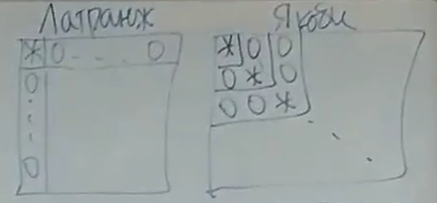
\includegraphics[height=5cm]{lecture20_matrix}
\end{center}


\subsection{Нормальный вид квадратичной формы над полем $\RR$}

\begin{definition}
    Квадратичная форма над $\RR$ имеет \textit{нормальный вид} в базисе $\E$, если в этом базисе
    \begin{equation*}
        Q(x_1, \dots, x_n) = \epsilon_1 x_1^2 + \dots + \epsilon_n x_n^2
    ,\end{equation*}
    где $\epsilon_i \in \{-1, 0, 1\}$.
\end{definition}


\subsection{Приведение квадратичной формы над R к нормальному виду}

\begin{corollary}[из метода Лагранжа]
    Для всякой квадратичной формы $Q$ над $\RR$ существует базис, в котором $Q$ имеет нормальный вид.
\end{corollary}

\begin{proof}
    Из теоремы знаем, что существует базис $\E$, в котором $Q$ имеет канонический вид
    \begin{equation*}
        Q(x_1, \dots, x_n) = b_1 x_1^2 + \dots + b_n x_n^2
    .\end{equation*}

    Делаем замену
    \begin{equation*}
        x_i = \begin{cases}
            \frac{x'_i}{\sqrt{|b_i|}}, &b_i \neq 0 \\
            x_i, &b_i = 0
        \end{cases}
    .\end{equation*}

    Тогда в новых координатах $Q(x'_1, \dots, x'_n) = \epsilon_1 x'^2_1 + \dots + \epsilon_n x'^2_n$,

    \begin{equation*}
        \epsilon_i = \sgn b_i = \begin{cases}
            1, &b_i > 0 \\
            0, &b_i = 0 \\
            -1, &b_i < 0
        \end{cases}
    .\end{equation*}
\end{proof}

    \section{Лекция 20.02.2020}

\begin{comment}
    Для $F = \CC$ всякую квадратичную форму можно привести к виду \eqref{lec21:1}, где $k = \rk Q$.
    \begin{equation}
        \label{lec21:1}
        Q = x_1^2 + \dots + x_k^2
    .\end{equation}
\end{comment}


\subsection{Положительный и отрицательный индексы инерции квадратичной формы над $\RR$}

Пусть $F = \RR$.

Пусть $Q \colon V \to \RR$ --- квадратичная форма.

Можно привести к нормальному виду
\begin{equation*}
    Q(x_1, \dots, x_n) = x_1^2 + \dots + x_s^2 - x_{s + 1}^2 - \dots - x_{s + t}^2
.\end{equation*}

Здесь
\begin{math}
    \begin{aligned}[t]
        &i_+ := s \text{ --- положительный индекс инерции квадратичной формы $Q$}, \\
        &i_- := t \text{ --- отрицательный индекс инерции квадратичной формы $Q$}.
    \end{aligned}
\end{math}


\subsection{Закон инерции}

\begin{theorem}
    Числа $i_+$ и $i_-$ не зависят от базиса в котором $Q$ принимает нормальный вид.
\end{theorem}

\begin{proof}
    $s + t = \rk Q$, то есть не зависит от выбора базиса. Следовательно, достаточно показать, что число $s$ определено однозначно.

    Пусть $\E = (e_1, \dots, e_n)$ --- базис, в котором $Q$ принимает нормальный вид
    \begin{equation*}
        Q = x_1^2 + \dots + x_s ^2 - x_{s + 1}^2 - \dots - x_{s + t}^2
    .\end{equation*}

    Пусть $\E' = (e'_1, \dots, e'_n)$ --- другой базис, в котором $Q$ принимает нормальный вид
    \begin{equation*}
        Q = x'^2_1 + \dots + x'^2_s - x'^2_{s + 1} - \dots - x'^2_{s + t}
    .\end{equation*}

    Предположим, что $s \neq s'$, можно считать что $s > s'$.

    Положим 
    \begin{math}
        \begin{aligned}[t]
            &L := \left< e_1, \dots, e_s \right>, \ \dim L = s, \\
            &L' := \left< e'_{s + 1}, \dots, e'_{s + t} \right>, \ \dim L' = n - s'.
        \end{aligned}
    \end{math}

    \bigskip
    Так как $L + K' \subseteq V$, то $\dim \left(L + L'\right) \leq n$.

    Тогда, $\dim \left(L \cap L'\right) \geq s + (n - s') - n = s - s' > 0$.

    \bigskip
    Значит, $\exists$ вектор $v \in L \cap L'$, такой что $v \neq 0$.

    Теперь: 
    \begin{enumerate}[nosep]
        \item Так как $v \in L$, то $Q(v) > 0$,
        \item Так как $v \in L'$, то $Q(v) \leq 0$.
    \end{enumerate}
 
    Противоречие.
\end{proof}


\subsection{Следствие метода Якоби о вычислении индексов инерции квадратичной формы над $\RR$}

Пусть $Q \colon V \to \RR$ --- квадратичная форма,

$\E = (e_1, \dots, e_n)$ --- базис,

$B = B(Q, \E)$, 

$\delta_k$ --- $k$-й угловой минор матрицы $B$.


\begin{corollary}[из метода Якоби]
    Пусть $\delta_k \neq 0 \ \forall k$. Тогда:

    Число $i_+$ равно количеству \underline{сохранений знака} в последовательности $1, \delta_1, \dots, \delta_n$.

    Число $i_-$ равно количеству \underline{перемен знака} в последовательности $1, \delta_1, \dots, \delta_n$.
\end{corollary}

\begin{proof}
    Метод Якоби $ \implies \exists $ базис, в котором $Q$ принимает канонический вид
    \begin{equation*}
        Q = \delta_1 x_1^2 + \frac{\delta_2}{\delta_1} x_2^2 + \dots + \frac{\delta_n}{\delta_{n - 1}} x_{n}^2
    .\end{equation*}

    Здесь, знак отношения $\frac{\delta_i}{\delta_{i - 1}}$ соответствует смене либо сохранению знака в рассматриваемой последовательности.

    По закону инерции, количества знаков $+$ и $-$ не изменяются от выбора базиса.
\end{proof}


\subsection{Положительно определённые, отрицательно определённые, неотрицательно определённые, неположительно определённые, неопределённые квадратичные формы над $\RR$}

\begin{definition}
    Квадратичная форма $Q$ над $\RR$ называется
\end{definition}
\begin{table}[H]
{\renewcommand{\arraystretch}{1.7}
    \begin{tabular}{c|c|c|c|c}
        Термин & Обозначение & Условие & Нормальный вид & Индексы инерции \\ \hline
        Положительно определённой & $Q > 0$ & $Q(x) > 0 \ \forall x \neq 0$ & $x_1^2 + \dots + x_n^2$ & $i_+ = n, i_- = 0$ \\ \hline
        Отрицательно определённой & $Q < 0$ & $Q(x) < 0 \ \forall x \neq 0$ & $-x_1^2 - \dots - x_n^2$ & $i_+ = 0, i_- = n$ \\ \hline
        Неотрицательно определённой & $Q \geq 0$ & $Q(x) \geq 0 \ \forall x$ & $x_1^2 + \dots + x_k^2, \ k \leq n$ & $i_+ = k, i_- = 0$ \\ \hline
        Неположительно определённой & $Q \leq 0$ & $Q(x) \leq 0 \ \forall x$ & $-x_1^2 - \dots - x_k^2, \ k \leq n$ & $i_+ = 0, i_- = k$ \\ \hline
        Неопределённой & --- & 
        \begin{math}
            \begin{aligned}
                \exists x : Q(x) > 0 \\
                \exists y : Q(y) < 0
            \end{aligned}
        \end{math} &
        \begin{math}
            \begin{gathered}
                x_1^2 + \dots + x_s ^2 - x_{s + 1}^2 - x_{s + t}^2 \\
                s, t \geq 1
            \end{gathered}
        \end{math} & $i_+ = s, i_- = t$
        \\ \hline
    \end{tabular}       
}
\end{table}


\subsection{Примеры}

$V = \RR^2$.

\begin{enumerate}
\item $Q(x, y) = x^2 + y^2$, $Q > 0$.

    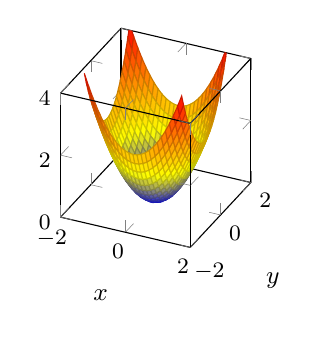
\begin{tikzpicture}
    \begin{axis}[
    xlabel=$x$, ylabel=$y$, small,
    xmin=-2, xmax=2,
    ymin=-2, ymax=2,
    zmin=0, zmax=4,
    3d box=complete,
    unit vector ratio*=1 1 1,
    ]
    \addplot3[surf, domain=-1.5:1.5] 
    {x^2+y^2};
    \end{axis}
    \end{tikzpicture} 

\item $Q(x, y) = -x^2 - y^2$, $Q < 0$.

    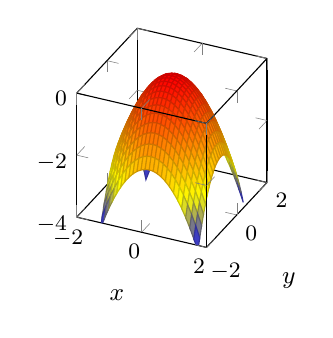
\begin{tikzpicture}
    \begin{axis}[
    xlabel=$x$, ylabel=$y$, small,
    xmin=-2, xmax=2,
    ymin=-2, ymax=2,
    zmin=-4, zmax=0,
    3d box=complete,
    unit vector ratio*=1 1 1,
    ]
    \addplot3[surf, domain=-1.5:1.5] 
    {-x^2-y^2};
    \end{axis}
    \end{tikzpicture} 

\item $Q(x, y) = x^2$, $Q \geq 0$.
    
    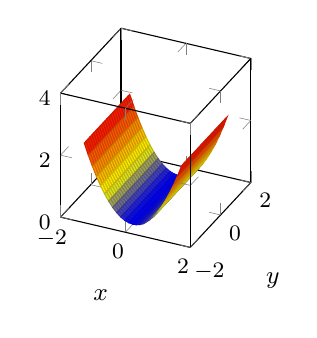
\begin{tikzpicture}
    \begin{axis}[
    xlabel=$x$, ylabel=$y$, small,
    xmin=-2, xmax=2,
    ymin=-2, ymax=2,
    zmin=0, zmax=4,
    3d box=complete,
    unit vector ratio*=1 1 1,
    ]
    \addplot3[surf, domain=-1.5:1.5] 
    {x^2};
    \end{axis}
    \end{tikzpicture} 

\item $Q(x, y) = -x^2$, $Q \leq 0$.

    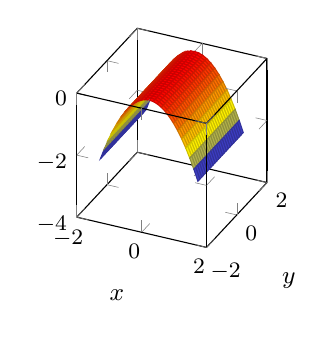
\begin{tikzpicture}
    \begin{axis}[
    xlabel=$x$, ylabel=$y$, small,
    xmin=-2, xmax=2,
    ymin=-2, ymax=2,
    zmin=-4, zmax=0,
    3d box=complete,
    unit vector ratio*=1 1 1,
    ]
    \addplot3[surf, domain=-1.5:1.5] 
    {-x^2};
    \end{axis}
    \end{tikzpicture} 

\item $Q(x, y) = x^2 - y^2$.

    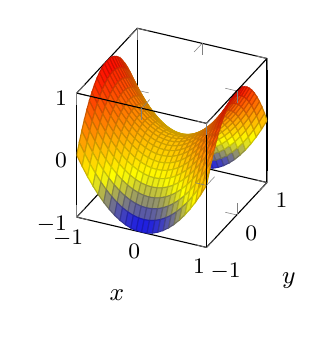
\begin{tikzpicture}
    \begin{axis}[
    xlabel=$x$, ylabel=$y$, small,
    xmin=-1, xmax=1,
    ymin=-1, ymax=1,
    zmin=-1, zmax=1,
    3d box=complete,
    unit vector ratio*=1 1 1,
    ]
    \addplot3[surf, domain=-1:1] 
    {x^2 - y^2};
    \end{axis}
    \end{tikzpicture} 

\end{enumerate}


\subsection{Критерий Сильвестра положительной определённости квадратичной формы}
\subsection{Критерий отрицательной определённости квадратичной формы}
\subsection{Евклидово пространство}
\subsection{Скалярное произведение}
\subsection{Примеры}


    \section{Лекция 20.02.2020}


\begin{comment}
    Всякое подпространство $U \subseteq E$ тоже является евклидовым пространством со скалярным произведением $(\bigcdot, \bigcdot) \big|_U \leftarrow$ ограничение на $U$.
\end{comment}


\subsection{Длина вектора евклидова пространства}

\begin{definition}
    \textit{Длина} вектора $x \in \EE$ --- это $|x| := \sqrt{(x, x)}$.

    Свойство: 
    $|x| \geq 0$, причем $|x| = 0 \iff x = 0$.
\end{definition}

\begin{example}
    Если $\EE = \RR^n$ со стандартным скалярным произведением, то $|x| = \sqrt{x_1^2 + \dots + x_n^2}$.
\end{example}

\begin{comment}
    Если $\EE = \text{Mat}_{m \times n}(\RR)$, $(A, B) = \tr(A^{T} B)$

    Тогда, $|A| = \sqrt{\sum_{i = 1}^{m} \sum_{j = 1}^{n} a_{ij}^2} \leftarrow$ это обозначается как $\norm{A}_{F}$ и называется \textit{нормой Фробениуса}, \textit{фробениусовой нормой}.
\end{comment}


\subsection{Неравенство Коши–Буняковского}

\begin{proposal}[неравенство Коши-Буняковского]
    $\forall x, y \in \EE$ верно $|(x, y)| \leq |x| \cdot |y|$, причём равенство $\iff$ $x$, $y$ пропорциональны.
\end{proposal}

\begin{proof}
    Случаи:
    \begin{enumerate}
    \item $x, y$ пропорциональны. Тогда, можно считать, что $y = \lambda x$, $\lambda \in \RR$.

        $|(x, y)| = |(x, \lambda x)| = |\lambda| |(x, x)| = |\lambda| |x|^2 = |x| \cdot |\lambda x| = |x| \cdot |y|$.

    \item $x, y$ не пропорциональны. Тогда $x, y$ линейно независимы.

        Значит они образуют базис в $\left< x, y \right>$.

        Получаем
        \begin{equation*}
            \begin{vmatrix} 
                (x, x) & (x, y) \\
                (y, x) & (y, y)
            \end{vmatrix} > 0 \quad \text{(критерий Сильвестра)}
        .\end{equation*}

        Отсюда, $(x, x) \cdot (y, y) - (x, y)^2 > 0 \implies (x, y)^2 < |x|^2 \cdot |y|^2$.
    \end{enumerate}
\end{proof}

\begin{example}
    Пусть $\EE = \RR^n$ со стандартным скалярным произведением, тогда
    \begin{equation*}
        |x_1 y_1 + \dots + x_n y_n| \leq \sqrt{x_1^2 + \dots + x_n^2} \cdot \sqrt{y_1^2 + \dots + y_n^2}
    .\end{equation*}
\end{example}


\subsection{Угол между ненулевыми векторами евклидова пространства}

Пусть $x, y \in \EE \setminus \{0\}$, тогда $-1 \leq \frac{(x, y)}{|x| \cdot |y|} \leq 1$.

\begin{definition}
    Угол между ненулевыми векторами $x, y \in \EE$, это такой $\alpha \in [0, \pi]$, что $\cos \alpha = \frac{(x, y)}{|x| \cdot |y|}$.

    Тогда $(x, y) = |x| |y| \cos \alpha$.
\end{definition}


\subsection{Матрица Грама системы векторов евклидова пространства}

Пусть $v_1, \dots, v_k$ --- произвольная система векторов.

\begin{definition}
    \textit{Матрица Грама} этой системы --- это
    \begin{equation*}
        G(v_1, \dots, v_k) = \begin{pmatrix}
            (v_1, v_1) & (v_1, v_2) & \dots & (v_1, v_k) \\
            (v_2, v_1) & (v_2, v_2) & \dots & (v_2, v_k) \\
            \vdots & \vdots & \ddots & \vdots \\
            (v_k, v_1) & (v_k, v_2) & \dots & (v_k, v_k)
        \end{pmatrix}
    .\end{equation*}
\end{definition}

\begin{example}
    $\EE = \RR^n$ со стандартным скалярным произведением.

    $a_1, \dots, a_k \in \RR^n \leadsto A := (a_1, \dots, a_k) \in \text{Mat}_{n \times k}(\RR)$.

    Тогда, $G(a_1, \dots, a_k) = A^T \cdot A$.
\end{example}


\subsection{Определитель матрицы Грама: неотрицательность, критерий положительности}

\begin{proposal}
    $\forall v_1, \dots, v_k \in \EE \implies \det G(v_1, \dots, v_k) \geq 0$.

    Более того, $\det G(v_1, \dots, v_k) > 0 \iff v_1, \dots, v_k$ линейно независимы. 
\end{proposal}

\begin{proof}
    Пусть $G := G(v_1, \dots, v_k)$.
    Случаи:
    \begin{enumerate}
    \item $v_1, \dots, v_k$ линейно независимы. Тогда, $G$ --- матрица билинейной формы $(\bigcdot, \bigcdot) \Big|_{\left< v_1, \dots, v_k \right>}$ в базисе $v_1, \dots, v_k$ подпространства $\left< v_1, \dots, v_k \right>$, а значит $\det G > 0$ по критерию Сильвестра.
    
    \item $v_1, \dots, v_k$ линейно зависимы. Тогда, $\exists (\alpha_1, \dots, \alpha_k) \in \RR^k \setminus \{0\}$, такие что $\alpha_1 v_1 + \dots + \alpha_k v_k = 0$.

        А значит,  $\forall i = 1, \dots, k \implies \alpha_1 (v_1, v_i) + \dots + \alpha_k (v_k, v_i) = 0$.
        
        Отсюда, $a_1 G_{(1)} + \dots + \alpha_k G_{(k)} = 0 \implies$ строки в $G$ линейно зависимы $\implies \det G = 0$.
        \qedhere
    \end{enumerate}
\end{proof}


\subsection{Ортогональные векторы}

\begin{definition}
    Векторы $x, y \in \EE$ называются \textit{ортогональными}, если $(x, y) = 0$.
\end{definition}


\subsection{Ортогональное дополнение подмножества евклидова пространства}

\begin{definition}
    \textit{Ортогональное дополнение} множества $S \subseteq \EE$ --- это множество $S^{\perp} := \{x \in \EE \mid (x, y) = 0 \forall y \in S\}$.
\end{definition}

\begin{exercise}~
    \begin{enumerate}
    \item $S^{\perp}$ --- подпространство в $\EE$.
    \item $S^{\perp} = \left< S \right>^{\perp}$.
    \end{enumerate}
\end{exercise}

\subsection{Размерность ортогонального дополнения подпространства, ортогональное дополнение к ортогональному дополнению подпространства}
\subsection{Разложение евклидова пространства в прямую сумму подпространства и его ортогонального дополнения}

Далее считаем, что $\dim \EE = n < \infty$.

\begin{proposal}
    Пусть $S \subseteq \EE$ --- подпространство.
    Тогда:
    \begin{enumerate}
    \item $\dim S^{\perp} = n - \dim S$.
    \item $\EE = S \oplus S^{\perp}$.
    \item $(S^{\perp})^{\perp} = S$.
    \end{enumerate}
\end{proposal}

\begin{proof}~
    \begin{enumerate}
    \item 
        Пусть $\dim S = k$ и $e_1, \dots, e_k$ --- базис $S$.
        
        Дополним $e_1, \dots, e_k$ до базиса $e_1, \dots, e_n$ всего $\EE$.

        Тогда, $\forall x = x_1 e_1 + \dots + x_n e_n \in \EE$.

        \begin{align*}
            x \in S^{\perp} &\iff (x, e_i) = 0 \ \forall i = 1, \dots, k \\
                            &\iff \begin{cases}
                                (e_1, e_1) x_1 + \dots + (e_n, e_1) x_n = 0 \\
                                (e_1, e_2) x_1 + \dots + (e_n, e_2) x_n = 0 \\
                                \dots \\
                                (e_1, e_k) x_1 + \dots + (e_n, e_k) x_n = 0
                            \end{cases}
        .\end{align*}

        Это ОСЛУ с матрицей $G \in \text{Mat}_{k \times n}(\RR)$, причём любой $k \times k$ блок в $G$ --- это $\underbrace{G(e_1, \dots, e_k)}_{\det \neq 0}$.

        Это означает, что $\rk G = k$.

        Следовательно, пространство решений этой ОСЛУ имеет размерность $n - k$.

        Отсюда, $\dim S^{\perp} = n - k = n - \dim S$.

    \item
        \begin{enumerate}
        \item $\dim S + \dim S^{\perp} = k + (n - k) = n = \dim E$.
        \item $v \in S \cap S^{\perp} \implies (v, v) = 0 \implies v = 0 \implies S \cap S^{\perp} = \{0\}$.
        \end{enumerate}

        А значит, $E = S \oplus S^{\perp}$.

    \item
        Заметим, что $S \subseteq (S^{\perp})^{\perp}$ (по определению).

        $\dim (S^{\perp})^{\perp} = n - \dim S^{\perp} = n - (n - \dim S) = \dim S$.

        Следовательно, $S = (S^{\perp})^{\perp}$.
        \qedhere
    \end{enumerate}
\end{proof}


\subsection{Ортогональная проекция вектора на подпространство, ортогональная составляющая вектора относительно подпространства}

$S$ --- подпространство $ \implies \EE = S \oplus S^{\perp}$

$\forall v \in \EE \exists! x \in S, y \in S^{\perp}$, такие что $x + y = v$.

\begin{definition}~
    \begin{enumerate}
    \item 
        $x$ называется \textit{ортогональной проекцией} вектора $v$ на подпространство $S$.

        Обозначение: $x = \pr_S v$.

    \item
        $y$ называется \textit{ортогональной составляющей} вектора $v$ относительно подпространства $S$.

        Обозначение: $y = \ort_S v$.
    \end{enumerate}
\end{definition}

\subsection{Явная формула для ортогональной проекции вектора на подпространство в $\RR^n$, заданное своим базисом}

Пусть $\EE = \RR^n$ со стандартным скалярным произведением.

$S \subseteq \EE$ --- подпространство, $a_1, \dots, a_k$ --- базис $S$.

Пусть $A := (a_1, \dots, a_k) \in \text{Mat}_{n \times k}(\RR)$, $A^{(i)} = a_i$.

\begin{proposal}
    $\forall v \in \RR^n \quad \pr_S v = A (A^{T} A)^{-1} A^{T} v$.
\end{proposal}

\begin{proof}
    Корректность: $A^{T} A = G(a_1, \dots, a_k) \in M_k^{0}(\RR)$.

    Положим $x := \pr_S v$, $y := \ort_S v$.

    Так как $x \in S$, $x = A \cdot \begin{pmatrix} \alpha_1 \\ \dots \\ \alpha_k \end{pmatrix}$, $\alpha_i \in \RR$.

    $y \in S^{\perp} \implies A^T y = 0$.

    \begin{align*}
    A (A^{T} A)^{-1} A^{T} v
    &= A(A^{T}A)^{-1}A^{T} (x + y) \\
    &= A\lefteqn{\underbracket{\phantom{(A^{T}A)^{-1}A^{T} A}}_E} (A^{T} A)^{-1} A^{T} \overbracket{A \begin{pmatrix} \alpha_1 \\ \dots \\ \alpha_k \end{pmatrix}}^{x} + A(A^{T} A)^{-1} \underbracket{A^{T} y}_{0} \\
    &= A \begin{pmatrix} \alpha_1 \\ \dots \\ \alpha_k \end{pmatrix} = x = \pr_S v
    .\end{align*}
\end{proof}


\subsection{Ортогональные и ортонормированные системы векторов}

\begin{definition}
    Система ненулевых векторов $v_1, \dots, v_k$ называется
    \begin{enumerate}[nosep]
        \item \textit{ортогональной}, если $(v_i, v_j) = 0 \ \forall i \neq j$ (то есть $G(v_1, \dots, v_k)$ диагональна),
        \item \textit{ортонормированной}, если $(v_i, v_j) = 0 \ \forall i \neq j$ и $(v_i, v_i) = 1$ ($\iff |v_i| = 1$).
            То есть $G(v_1, \dots, v_k) = E$.
    \end{enumerate}
\end{definition}

\begin{comment}
    Всякая ортогональная (и в частности ортонормированная) система векторов автоматически линейно независима.
    \begin{equation*}
        \det G(v_1, \dots, v_k) = |v_1|^2 \dots |v_k|^2 \neq 0
    .\end{equation*}
\end{comment}


\subsection{Ортогональный и ортонормированный базис}

\begin{definition}
    Базис пространства называется \textit{ортогональным} (соответственно \textit{ортонормированным}), если он является ортогональной (ортонормированной) системой векторов.
\end{definition}

    \section{Лекция 1.03.2018}

$E$ -- евклидово пространство

\textbf{Определение.} Система ненулевых векторов $(v_1, \dots, v_k)$ пространства $E$ называется:

-- \textit{ортогональной}, если $(v_i, v_j) = 0 \ \forall \ i \neq j$ (т.е. $G(v_1, \dots, v_k)$ диагональна)

-- \textit{ортонормированной}, если $(v_i, v_j) = 0 \ \forall i \neq j$ и $(v_i, v_i) = 1 \ \forall \ i \ (|v_i| = 1)$ (т.е. $G(v_1, \dots, v_k) = E$)

\bigskip
\textbf{Замечание.} Всякая ортогональная система векторов линейно независима (т.к. $det G(v_1, \dots, v_k) = |v_1|^2 \cdot \dots \cdot |v_k|^2 \neq 0$). В частности, всякая ортонормированная система векторов линейно независима.

\bigskip
\textbf{Определение.} Базис $(e_1, \dots, e_n)$ пространства $E$ называется \textit{ортогональным (соответственно ортонормированным)}, если система векторов $(e_1, \dots, e_n)$ ортогональна (соответсвенно ортонормированна).

\bigskip
Пример. 
$E = \RR^n$ со стандартным скалярным произведением. Тогда стандартный базис $e_1 = \begin{pmatrix} 1 \\ 0 \\ \vdots \\ 0 \end{pmatrix}, e_2 = \begin{pmatrix} 0 \\ 1 \\ \vdots \\ 0 \end{pmatrix}, \dots, e_n = \begin{pmatrix} 0 \\ 0 \\ \vdots \\ 1 \end{pmatrix}$ является ортонормированным.

\bigskip
\textbf{Теорема.} Во всяком (конечномерном) евклидовом пространстве есть ортонормированный базис.

\bigskip
\textbf{\textit{Доказательство.}} $\rhd$ Следует из теоремы о нормальном виде для квадратичной формы $(x, x) \ \lhd$.

\bigskip
\textbf{Следствие.} Всякую ортогональную (ортонормированную) систему векторов $e_1, \dots, e_k$  можно дополнить до ортогонального (ортонормированного) базиса в $E$.

\bigskip
\textbf{\textit{Доказательство.}} $\rhd$ Достаточно взять ортогональный (ортонормированный) базис в подпространстве $<e_1, \dots, e_k>^{\bot} \ \lhd$

\bigskip
$(e_1, \dots, e_n)$ -- ортогональный базис

$(e'_1, \dots, e'_n)$ -- другой базис

$(e'_1, \dots, e'_n) = (e_1, \dots, e_n) \cdot C$ -- матрица перехода

\bigskip
\textbf{Предложение.} Базис $(e'_1, \dots, e'_n)$ ортонормированный $\Leftrightarrow C^T C = E$

\bigskip
\textbf{\textit{Доказательство.}} $\rhd$ Имеем $G^T G(e_1, \dots, e_n) C = C^T C$ $(G(e_1, \dots, e_n) = E)$

$(e'_1, \dots, e'_n)$ ортонормированный $\Leftrightarrow G(e'_1, \dots, e'_n) = E \ \lhd$

\bigskip
\textbf{Определение.} Матрица $C \in M_n (\RR)$ называется \textit{ортогональной}, если $C^T C = E$.

\bigskip
\textbf{Замечание.} $C^T C = E \Leftrightarrow C^T = C^{-1} \Leftrightarrow C C^T = E$

\bigskip
\textbf{\textit{Свойства:}}

1) $(C^{(i)}, C^{(j)}) = \delta_{ij}$ (т.е. столбцы $C$ -- это ортонормированная система в $\RR^n$)

2) $(C_{(i)}, C_{(j)}) = \delta_{ij}$ (т.е. строки $C$ -- это ортонормированная система в $\RR^n$)

В частности, $|c_{ij}| \leq 1$

3) $(det C)^2 = 1 \Leftrightarrow detC = \pm 1$

\bigskip
Пример.

$n = 2$

$\begin{pmatrix} \cos \varphi & - \sin \varphi \\
\sin \varphi & \cos \varphi \end{pmatrix}, det = 1$

$\begin{pmatrix} \cos \varphi & \sin \varphi \\
\sin \varphi & - \cos \varphi \end{pmatrix}, det = -1$

\bigskip
$S \subseteq E$ -- подпространство, $(e_1, \dots, e_k)$ -- ортогональный базис в $S$

\bigskip
\textbf{Предложение.} $v \in E \Rightarrow pr_S v = \sum\limits_{i=1}^k \frac{(v, e_i)}{(e_i, e_i)} e_i$. Если $(e_1, \dots, e_k)$ ортонормированный, то $pr_S v = \sum\limits_{i=1}^k (v, e_i) e_i$

\bigskip
\textbf{\textit{Доказательство.}} $\rhd \ v = pr_S v + ort_S v \Rightarrow \forall \ i = 1, \dots, k \ (v, e_i) = (pr_S v, e_i)$

$pr_S v = \sum\limits_{j = 1}^k \lambda_j e_j \Rightarrow (v, e_i) = (pr_S v, e_i) = \sum\limits_{j = 1}^n \lambda_j (e_i, e_i) = \lambda_i (e_i, e_i) \Rightarrow \lambda_i = \frac{(v, e_i)}{(e_i, e_i)} \ \lhd$.

\bigskip
$(e_1, \dots, e_k)$  -- линейно независимая система векторов

Метод Якоби $\Rightarrow \exists!$ ортогональная система $(f_1, \dots, f_k)$, такая что

\begin{equation*}
(*) \begin{cases}
		f_1 = e_1 \\
		f_2 \in e_2 + <e_1> \\
        f_3 \in e_3 + <e_1, e_2> \\
        \vdots \\
        f_n \in e_k + <e_1, \dots, e_{k-1}>
	\end{cases}
\end{equation*}  

\bigskip
\textbf{Предложение.} $\forall \ i = 1, \dots, k$

1) $f_i = ort_{<e_1, \dots, e_{i-1}>} e_i$

2) $f_i = e_i - \sum\limits_{j=1}^{i-1} \frac{(e_i, f_j)}{(f_j, f_j)} f_j$ (**)

3) $det G(e_1, \dots, e_i) = det G(f_1, \dots, f_i)$

\bigskip
\textbf{\textit{Доказательство.}} $\rhd$ Знаем, что $<e_1, \dots, e_i> = <f_1, \dots, f_i>$

$f_i \in e_i + <e_1, \dots, e_{i-1}> = e_i + <f_1, \dots, f_{i-1}> \Rightarrow f_i = e_i + h_i$, где $h_i \in <f_1, \dots, f_{i-1}> \Rightarrow e_i = f_i - h_i$. Т.к. $f_i \in <f_1, \dots, f_{i-1}>^{\bot}$, то $f_i = ort_{<f_1, \dots, f_{i-1}>} e_i = ort_{<e_1, \dots, e_{i-1}>} e_i$.

2) $f_i = e_i - pr_{<e_1, \dots, e_{i-1}>} e_i = e_i - pr_{<f_1, \dots, f_{i-1}>} e_i = e_i - \sum\limits_{j=1}^{i-1} \frac{(e_i, f_j)}{(f_j, f_j)} f_j$.

3) Было $\lhd$

\bigskip
Процесс простроения ортогонального базиса $f_1, \dots, f_k$ по формулам (**) называется \textit{процессом (или методом) ортогонализации Грама-Шмидта}.

\bigskip
\textbf{\textit{Упражнение.}} Модифицировать метод ортогонализации Грама-Шмидта для случая линейно зависимой системы векторов.

\bigskip
\textbf{Предложение (теорема Пифагора).} $x, y \in E, (x, y) = 0 \Rightarrow |x+y|^2 = |x|^2 + |y|^2$.

\bigskip
\textbf{\textit{Доказательство.}} $\rhd \ |x+y|^2 = (x+y, x+y) = (x,x) + (x,y) + (y,x) + (y,y) = |x|^2 + |y|^2 \ \lhd$.

\bigskip
\textbf{Определение.} \textit{Расстоянием между векторами} $x, y \in E$ называется число $\rho (x, y) := |x - y|$. 

\bigskip
\textbf{Предложение (неравенство треугольника).} $\forall \ a, b, c \in E \rho(a, b) + \rho(b, c) \geq \rho(a, c)$.

\bigskip
\textbf{\textit{Доказательство.}} $\rhd$ Положим $x = a - b, y = b - c$, тогда $a - c = x + y \Rightarrow$  надо доказать $|x| + |y| \geq |x + y|$

$|x + y|^2 = (x+y, x+y) = (x,x) + 2(x,y) + (y,y) \leq |x|^2 + 2 |x| |y| + |y|^2 \leq (|x| + |y|)^2 \ \lhd$

\bigskip
$P, Q \subseteq E$ -- два непустых подмножества

\textbf{Определение.} \textit{Расстояние между} $P$ и $Q$ -- это $\rho(P, Q) := inf \rho (x, y), x \in P, y \in Q$

\bigskip
Пусть $v \in E$ и $S \subseteq E$ -- подпространство

\textbf{Теорема.} $\rho (v, S) = |ort_S v|$, причем $pr_S v$ есть единственный ближайший к $v$ вектор из $S$. 

\bigskip
\textbf{\textit{Доказательство.}} $\rhd$ Пусть $z = ort_S v, u = pr_S v$.

Тогда $v = z + y$. Пусть $y' \in S, y' \neq 0$. Тогда $\rho (v, y + y')^2 = |v - y - y'|^2 = |z - y'|^2 =$ (теорема Пифагора) $= |z|^2 + |y'|^2 > |z|^2 = |v - y|^2 = \rho (v, y)^2 \ \lhd$.


    \section{Лекция 15.03.2018}

$E$ -- евклидово пространство, $dimE = n$

$x \in E, S \subseteq E$ -- подпространство

\vspace{\baselineskip}
\subsection{Метод наименьших квадратов}

$(*) Ax = b$, $A \in Mat_{m \times n}, \ x \in \mathbb{R}^n$ -- столбец неизвестных, $b \in \mathbb{R}^m$ -- столбец правых частей

$x$ -- решение СЛУ (*) $\Leftrightarrow Ax = b \Leftrightarrow |Ax - b| = 0 \Leftrightarrow \rho (Ax, b) = 0$

\vspace{\baselineskip}
\textbf{Определение.} Если СЛУ(*) несовместна, то $x_0 \in \mathbb{R}^n$ называется ее \textit{псевдорешением}, если $\rho(Ax_0, b) = min (\rho(Ax, b))$ (иначе говоря, $x_0$ -- решение задачи оптимизации $\rho(Ax, b) \rightarrow min$)

\vspace{\baselineskip}
Пусть $S \subseteq \mathbb{R}^m$ -- подпространство, натянутое на столбцы матрицы $A$, т.е. $S = <A^{(1)}, \dots, A^{(n)}>$, $c := pr_S b$.

\vspace{\baselineskip}
\textbf{Предложение.} 1) $x_0$ -- псевдорешение для (*) $\Leftrightarrow Ax_0 = c$

2) Если столбцы $A^{(1)}, \dots, A^{(n)}$ линейно независимы, то $x_0$ можно найти по формуле $x_0 = (A^T A)^{-1} A^T b$

\vspace{\baselineskip}
\textbf{\textit{Доказательство.}} $\rhd$ 1) $x \in \mathbb{R}^n \Rightarrow Ax = x_1 A^{(1)} + \dots + x_n A^{(n)}$

$x = \begin{pmatrix} x_1 \\ \vdots \\ x_n \end{pmatrix} \Rightarrow Ax = S$

$min( \rho (Ax, b)) = \rho (S, b)$

\vspace{\baselineskip}
По предыдущей теореме получаем, что $x_0$ -- псведорешение $\Leftrightarrow Ax_0 = c$

\vspace{\baselineskip}
2) т.к. столбцы $A$ линейно независимы, то $x_0$ единственный. Знаем, что $c = A (A^T A)^{-1} A^T b$. Но тогда $x_0 = (A^T A)^{-1} A^T b$ является решением СЛУ $Ax = c \ \lhd$

\vspace{\baselineskip}
Пример.

СЛУ $\begin{cases}
		x = 0 \\
		x = 1
	\end{cases}$, $A = \begin{pmatrix} 1 \\ 1 \end{pmatrix}, \ b = \begin{pmatrix} 0 \\ 1 \end{pmatrix}$

\vspace{\baselineskip}
$x_0 = (A^T A)^{-1} A^T b = \frac{1}{2}$

\vspace{\baselineskip}
$S \subseteq E$ - подпространство, $x \in E$

$e_1, \dots, e_k$ -- базис $S$

\vspace{\baselineskip}
\textbf{Теорема.} $\rho (x, S)^2 = \frac{det G(e_1, \dots, e_k, x)}{det G(e_1, \dots, e_k)}$

\vspace{\baselineskip}
\textbf{\textit{Доказательство.}} $\rhd$ 1) $x \in S \Rightarrow \rho (x, S) = 0, \ det G(e_1, \dots, e_k, x) = 0$, т.к. $e_1, \dots, e_k, x$ линейно независимы

\vspace{\baselineskip}
2) $x \notin S$. Пусть $z = ort_S x$, тогда $\rho(x, s)^2 = |z|^2$.

Применив процесс ортогонализации к системе $e_1, \dots, e_k, x$, получим ортогональную систему $f_1, \dots, f_k, z$. При ортогонализации определитель матрицы Грама не меняется $\Rightarrow \frac{det G(e_1, \dots, e_k, x)}{det G(e_1, \dots, e_k)} = \frac{det G(f_1, \dots, f_k, z)}{det G(f_1, \dots, f_k)} = \frac{|f_1|^2 |f_2|^2 \dots |f_k|^2 |z|^2}{|f_1|^2 |f_2|^2 \dots |f_k|^2} = |z|^2 \ \lhd$

\vspace{\baselineskip}
\textbf{Определение.} \textit{$k$-мерный параллелепипед, натянутый на векторы $a_1, \dots, a_k \in E$} -- это множество $P(a_1, \dots, a_k) = \{ x_1 a_1 + \dots + x_k a_k \ | \ 0 \leq x_i \leq 1 \}$. 

\vspace{\baselineskip}
Примеры.

1) $k = 1$  отрезок

2) $k = 2$ параллелограм

3) $k = 3$ параллелепипед

\vspace{\baselineskip}
$P(a_1, \dots, a_k)$ -- $k$-мерный параллелепипед

Основание: $P(a_1, \dots, a_{k-1})$

Высота: $h = ort_{<a_1, \dots, a_{k-1}>} a_k$

\vspace{\baselineskip}
\textbf{Определение.} \textit{$k$-мерный объем $k$-мерного параллелепипеда} $P(a_1, \dots, a_k)$ -- это величина \\ $vol(P(a_1, \dots, a_k))$, определяемая индуктивно по $k$.

\vspace{\baselineskip}
$k = 1 \Rightarrow vol(P(a_1)) := |a_1|$

$k > 1 \Rightarrow vol(P(a_1, \dots, a_k)) := vol(P(a_1, \dots, a_{k-1})) \cdot |h|$

\vspace{\baselineskip}
\textbf{Теорема.} $(vol(P(a_1, \dots, a_k)))^2 = det G(a_1, \dots, a_k)$

\vspace{\baselineskip}
\textbf{\textit{Доказательство.}} $\rhd$ Индукция по $k$. 

1) $k = 1: |a_1|^2 = (a_1, a_1)$ -- верно

2) $k > 1$

$(vol(P(a_1, \dots, a_k)))^2 = (vol(P(a_1, \dots, a_{k-1})))^2 \cdot |h|^2 = det G(a_1, \dots, a_{k-1}) \cdot |h|^2 = (*)$

Если $a_1, \dots, a_{k-1}$ линейно зависимы, то $det G(a_1, \dots, a_{k-1}) = 0 \Rightarrow (*) = 0$. Тогда $a_1, \dots, a_k$ тоже линейно зависимы $\Rightarrow det G(a_1, \dots, a_k) = 0$.

Если $a_1, \dots, a_{k-1}$ линейно независимы, то $|h|^2 = \frac{det G(a_1, \dots, a_{k-1}, a_k}{det G(a_1, \dots, a_{k-1}} \Rightarrow (*) = det G(a_1, \dots, a_k) \ \lhd$

\vspace{\baselineskip}
\textbf{Следствие.} Объем $k$-мерного параллелепипеда не зависит от выбора его основания.

\vspace{\baselineskip}
Пример.

Прямоугольный параллелепипед: $a_i \bot a_j \ \forall \ i \neq j$

$(vol(P(a_1, \dots, a_k)))^2 = det G(a_1, \dots, a_k) = |a_1|^2 |a_2|^2 \dots |a_k|^2 \Rightarrow vol(P(a_1, \dots, a_k)) = |a_1||a_2| \dots |a_k|$

\vspace{\baselineskip}
$(e_1, \dots, e_n)$ -- ортогональный базис в $E$

$a_1, \dots, a_n \in E$

$(a_1, \dots, a_n) = (e_1, \dots, e_n) \cdot A, \ A \in M_n (\mathbb{R})$

\vspace{\baselineskip}
\textbf{Теорема.} $vol P(a_1, \dots, a_n) = |det A|$

\vspace{\baselineskip}
\textbf{\textit{Доказательство.}} $\rhd \ (vol(P(a_1, \dots, a_n)))^2 = det G(a_1, \dots, a_n) = det (A^T A) = (det A)^2 \ \lhd$

\vspace{\baselineskip}
$e = (e_1, \dots, e_n)$ и $e' = (e'_1, \dots, e'_n)$ -- два базиса в $E$

$e' = e \cdot C, \ detc \neq 0$

\vspace{\baselineskip}
\textbf{Определение.} Базисы $e$ и $e'$ называются \textit{одинаково ориентированными}, если $detC > 0$.

\vspace{\baselineskip}
\textbf{Предложение.} 1) Отношение одинаковой ориентированности является отношением эквивалентности на множестве всех базисов в $E$

2) Имеется ровно 2 класса эквивалентности для этого отношения

\vspace{\baselineskip}
\textbf{\textit{Доказательство: упражнение.}}

\vspace{\baselineskip}
\textbf{Определение.} Говорят, что в $E$ задана ориентация, если все базисы одного класса объявлены положительно ориентированными, а все базисы второго класса объявлены отрицательно ориентированными.

\vspace{\baselineskip}
Базовый пример ориентации в $\mathbb{R}^3$:

-- положительно ориентированы "правые тройки векторов"

-- отрицательно ориентированы "левые тройки векторов"

\vspace{\baselineskip}
Фиксируем ориентацию в $E$

$(e_1, \dots, e_n)$ -- положительно ориентированный базис в $E$

\vspace{\baselineskip}
$a_1, \dots, a_n \in E$

$(a_1, \dots, a_n) = (e_1, \dots, e_n) \cdot A, \ A \in M_n(\mathbb{R})$

\vspace{\baselineskip}
\textbf{Определение.} \textit{Ориентированным объемом параллелепипеда} $P(a_1, \dots, a_n)$ называется величина $Vol(P(a_1, \dots, a_n)) = det A$. Информация об объеме + ориентации векторов $a_1, \dots, a_n$.

\vspace{\baselineskip}
\textbf{Следствие.} 1) $Vol(P(a_1, \dots, a_n)) > 0 \Leftrightarrow (a_1, \dots, a_n)$ -- положительно ориентированный базис $E$

$Vol(P(a_1, \dots, a_n)) < 0 \Leftrightarrow (a_1, \dots, a_n)$ -- отрицательно ориентированный базис $E$

2) $Vol(P(a_1, \dots, a_n))$ линеен по каждому аргументу (полилинеен)

3) Кососимметричность (при перестановке двух аргументов меняется знак)


    \section{Лекция 22.03.2018}

\subsection{Элементы аналитической геометрии в $\RR^3$}

$E =\RR^3$ со стандартным скалярным произведением, фиксируем ориентацию 

\vspace{\baselineskip}
\textbf{Определение.} \textit{Векторным произведением} двух векторов $a, b \in \RR^3$ называется вектор $c \in \RR^3$, удовлетворяющий следующим условиям:

1) $c \ \bot <a, b>$

2) $|c| = vol (P(a, b))$

3) $Vol(a, b, c) \geq 0$

Обозначение: $[a, b]$ или $a \times b$

\vspace{\baselineskip}
\textbf{Замечание.} Определение корректно, т.е. $\forall \ a, b \ \exists! \ c$,  удовлетворяющий 1)-3)

$a, b$ пропорциональны $\Rightarrow |c| = 0$ из 2) $\Rightarrow c = 0$

$a, b$ не пропорциональны $\Rightarrow$ 1) задает прямую, 2) задает $|c|$, 3) выбирает один из двух оставшихся вариантов

\vspace{\baselineskip}
\textbf{\textit{Критерий коллинеарности:}}

$a, b$ коллинеарны (= пропорциональны, = линейно зависимы) $\Leftrightarrow [a, b] = 0$

\vspace{\baselineskip}
Пример. $(e_1, e_2, e_3)$ -- положительно ориентированный ортонормированный базис

\vspace{\baselineskip}
\begin{tabular}{c|c|c|c}
$[e_i, e_j]$ & $e_1$ & $e_2$ & $e_3$ \\
\hline
$e_1$ & 0 & $e_3$ & $-e_2$  \\
\hline
$e_2$ & $-e_3$ & 0 & $e_1$   \\
\hline
$a_3$ & $e_2$ & $-e_1$ & 0   \\
\hline
\end{tabular}

\vspace{\baselineskip}
\textbf{Определение.} \textit{Смешанным произведением трех векторов} $a, b, c \in \RR^3$ называется число $(a, b, c) := (a, [b, c])$.

\vspace{\baselineskip}
\textbf{Теорема.} $(a, b, c) = Vol(a, b, c)$

\vspace{\baselineskip}
\textbf{\textit{Доказательство.}} $\rhd$ 1) $b, c$ пропорциональны $\Rightarrow$ обе части равны 0

2) $b, c$ не пропорциональны. Положим $d = [b, c]$. 

$(a, [b, c]) = (a, d) = (pr_{<d>} a, d) = (ort_{<b, c>}a, d) = \begin{cases}
		|ort_{<b, c>} a| \cdot |d|, \ если \ Vol(a, b, c) \geq 0 \\
		-|ort_{<b, c>} a| \cdot |d|, \ если \ Vol(a, b, c) \leq 0 \\
	\end{cases} = Vol(a, b, c)$

$\left[Vol(a, b, c) = Vol(pr_{<b, c>}a + ort_{<b, c>}a, b, c) = Vol(ort_{<b>}a, b, c)\right] \ \lhd$

\vspace{\baselineskip}
\textbf{Следствие (свойства смешанного произведения).}

1) $(a, b, c) > 0 \Leftrightarrow a, b, c$ образуют положительно ориентированный базис 

$(a, b, c) < 0 \Leftrightarrow a, b, c$ образуют отрицательно ориентированный базис

\vspace{\baselineskip}
\textbf{\textit{Критерий компланарности:}} $a, b, c$ компланарны (=линейно зависимы) $\Leftrightarrow (a, b, c) = 0$

2) $(a, b, c)$ линейно по каждому аргументу

3) $(a, b, c)$ кососимметрично

4) Если $e_1, e_2, e_3$ -- положительно ориентированный ортонормированный базис 

$a = a_1 e_1 + a_2 e_2 + a_3 e_3$

$b = b_1 e_1 + b_2 e_2 + b_3 e_3$

$c = c_1 e_1 + c_2 e_2 + c_3 e_3$

$\Rightarrow (a, b, c) = \begin{vmatrix} a_1 & a_2 & a_3 \\ b_1 & b_2 & b_3 \\ c_1 & c_2 & c_3 \end{vmatrix}$

\vspace{\baselineskip}
\textit{\textbf{Доказательство.}} Следует из свойств функции $Vol$.

\vspace{\baselineskip}
\textbf{Следствие.} $(a, [b, c]) = ([a, b], c)$

\vspace{\baselineskip}
\textbf{\textit{Доказательство.}} $\rhd \ (a, [b, c]) = (a, b, c) = (c, a, b) = (c, [a, b]) = ([a, b], c) \ \lhd$

\vspace{\baselineskip}
\textbf{Предложение.} 1) $[a, b] = -[b, a]$ (антикоммутативность)

2) $[\cdot, \cdot]$ линейно по каждому аргументу

$[\lambda_1 a_1 + \lambda_2 a_2, b] = \lambda_1 [a_1, b] + \lambda_2 [a_2, b]$

$[a, \mu_1 b_1 + \mu_2 b_2] = \mu_1 [a, b_1] + \mu_2 [a, b_2]$

\vspace{\baselineskip}
\textbf{\textit{Доказательство.}} $\rhd$ 1) из определения

2) $u = [\lambda_1 a_1 + \lambda_2 a_2, b]$

$v = \lambda_1 [a_1, b] + \lambda_2 [a_2, b]$

$\forall x \in \RR^3 : \ (x, u) = (x, \lambda_1 a_1 + \lambda_2 a_2, b) = \lambda_1 (a, a_1, b) + \lambda_2 (x, a_2, b) = \lambda_1 (x, [a_1, b]) + \lambda_2 (x, [a_2, b]) = (x, v) \Rightarrow u = v \ (e_1, e_2, e_3$ -- ортонормированный базис $\Rightarrow \ \forall \ y \in \RR^3 : \ y = (y_1, e_1) e_1 + (y_2, e_2) e_2 + (y_3, e_3) e_3)$

Аналогично линейность по второму аргументу $\lhd$.

\vspace{\baselineskip}
\textbf{Предложение (двойное векторное произведение).} $[a, [b, c]] = (a, c) b - (a, b) c$ ($= (b (a, c) - c (a, b)$ БАЦ-ЦАБ)

\vspace{\baselineskip}
\textbf{\textit{Доказательство.}} $\rhd$ 1) $b, c$ пропорциональны, пусть $c = \lambda b \Rightarrow [a, [b, c]] = 0$

$(a, c)b - (a, b) c = (a, \lambda b)b - (a, b) \lambda b = 0$

2) $b, c$ не пропорциональны

Выберем положительно ориентированный ортонормированный базис в $\RR^3$ так, что $e_1 \in <b>, e_2 \in <b, c>$. Тогда $b = \beta e_1, \ c = \gamma_1 e_1 + \gamma_2 e_2, \ a = \alpha_1 e_1 + \alpha_2 e_2 + \alpha_3 e_3$

$[b, c] = \beta \gamma_2 e_3$

$[a, [b, c]] = [\alpha_1 e_1 + \alpha_2 e_2 + \alpha_3 e_3, \beta \gamma_2 e_3] = -\alpha_1 \beta \gamma_2 e_2 + \alpha_2 \beta \gamma_2 e_1$

$(a, c) b - (a, b) c = (\alpha_1 \gamma_1 + \alpha_2 \gamma_2) \beta e_1 - \alpha_1 \beta (\gamma_1 e_1 + \gamma_2 e_2) = \alpha_2 \gamma_2 \beta e_1 - \alpha_1 \beta \gamma_2 e_2 \ \lhd$

\vspace{\baselineskip}
\textbf{Следствие (тождество Якоби).} $[a, [b, c]] + [b, [a, c]] + [c, [a, b]] = 0$

\vspace{\baselineskip}
\textbf{Предложение.} Пусть $e_1, e_2, e_3$ -- положительно ориентированный ортонормированный базис в $\RR^3$

$a = a_1 e_1 + a_2 e_2 + a_3 e_3$

$b = b_1 e_1 + b_2 e_2 + b_3 e_3$

Тогда $[a, b] = \begin{vmatrix} e_1 & e_2 & e_3 \\ a_1 & a_2 & a_3 \\ b_1 & b_2 & b_3 \end{vmatrix} = (a_2 b_3 - a_3 b_2) e_1 + (a_3 b_1 - a_1 b_3) e_2 + (a_1 b_2 - a_2 b_1) e_3 = \begin{vmatrix} a_2 & a_3 \\ b_2 & b_3 \end{vmatrix} e_1 - \begin{vmatrix} a_1 & a_3 \\ b_1 & b_3 \end{vmatrix} e_2 - \begin{vmatrix} a_1 & a_2 \\ b_1 & b_2 \end{vmatrix} e_3 $

\vspace{\baselineskip}
\textbf{\textit{Доказательство.}} Воспользоваться билинейностью и таблицей значений $[e_i, e_j]$.

\vspace{\baselineskip}
\textbf{Определение.} \textit{Линейным многообразием} в $\RR^n$ называется множество решений совместной СЛУ $Ax = b, \ \varnothing \neq L \subseteq \RR^n$

\vspace{\baselineskip}
Было:
\textbf{Лемма.} $L = x_0 + S$, где $x_0$ -- частное решение (= какое-то одно), $S$ -- пространство решений ОСЛУ $Ax = 0$

\vspace{\baselineskip}
\textbf{Предложение.} Множество $L \subseteq \RR^n$ является линейным многообразием $\Leftrightarrow L = v_0 + S$, где $S \subseteq \RR^n$ -- подпространство

\vspace{\baselineskip}
\textbf{\textit{Доказательство.}} $\rhd \ (\Rightarrow)$ следует из леммы

$(\Leftarrow)$ Знаем, что $S$ -- множество решений некоторой ОСЛУ $Ax = 0$. Тогда $L$ -- множество решений СЛУ $Ax = A v_0$ -- из леммы $\lhd$

\vspace{\baselineskip}
\textbf{Предложение.} Пусть $L_1 = v_1 + S_1$ и $L_2 = v_2 + S_2$. Тогда $L_1 = L_2 \Leftrightarrow \begin{cases} S_1 = S_2 (= S) \\ v_1 - v_2 \in S \end{cases}$

\vspace{\baselineskip}
\textbf{\textit{Доказательство.}} $\rhd \ (\Leftarrow)$ очевидно

$(\Rightarrow) v_1 = v_1 + 0 \in L_1$ и $v_1 + 0 \in v_2 + S_2 \Rightarrow v_1 - v_2 \in S_2$

$v \in S_1 \Rightarrow v_1 + v \in v_2 + S_2 \Rightarrow v \in (v_2 - v_1) + S_2 \subseteq S_2 \Rightarrow S_1 \subseteq S_2$

Аналогично $S_2 \subseteq S_1 \Rightarrow S_1 = S_2 (=S) \Rightarrow v_1 - v_2 \in S \ \lhd$

\vspace{\baselineskip}
$L = v_0 + S$ -- линейное многообразие $\Rightarrow S$ однозначно определяет пространство в $\RR^n$

\vspace{\baselineskip}
\textbf{Определение.} $S$ называется \textit{направляющим подпространством} линейного многообразия $L$.

\vspace{\baselineskip}
\textbf{Определение.} \textit{Размерностью} линейного многообразия называется размерность его направляющего подпространства.

Линейные многообразия размерности 0 -- это точки

Линейные многообразия размерности 1 называются прямые

Линейные многообразия размерности 2 называются плоскостями

Линейные многообразия размерности k называются k-мерными плоскостями


    \section{Лекция 09.04.2020} 

Если у вас ощущение, что в конспекте баг, можете проверить \href{https://www.dropbox.com/s/fty6fb2vuyugzdk/LA_19-20_osn_Lecture26.svg?dl=0}{снимок доски} и/или \href{https://youtu.be/U-UZGNDM1SA}{запись}.

\subsection{Теорема о плоскости, проходящей через любые $k+1$ точек в $\RR^n$, следствия для двух и трёх точек}

\begin{theorem}~
    \begin{enumerate}[label=\alph*)]
    \item Через любые $k + 1$ точек в $\RR^n$ проходит плоскость размерности $\leq k$.
    \item Если это точки не лежат в плоскости размерности $<k$, то через них проходит ровно одна плоскость размерности $k$.
    \end{enumerate}
\end{theorem}

\begin{proof}~
    \begin{enumerate}[label=\alph*)]
        \item Пусть $v_0, v_1, \dots, v_k$ --- данные точки. Тогда через них проходит плоскость $P = v_0 + \left< v_1 - v_0, \dots, v_k - v_0 \right>$.

            Ясно, что $\dim P \leq k$.

        \item Из условия следует, что $\dim P = k \implies v_1 - v_0, \dots, v_k - v_0$ линейно независимы.

            Если $P' = v_0 + S$ --- другая плоскость размерности $k$, содержащая $v_0, \dots, v_k$, то $v_1 - v_0, \dots, v_k - v_0 \in S \implies S = \left< v_1 - v_0, \dots, v_k - v_0 \right> \implies P' = P$.
            \qedhere
    \end{enumerate}
\end{proof}

\begin{corollary}~
    \begin{enumerate}
    \item Через любые две различные точки проходит ровно одна прямая.
    \item Через любые три точки, не лежащие на одной прямой, проходит ровно одна плоскость.
    \end{enumerate}
\end{corollary}


\subsection{Понятия репера и аффинной системы координат на линейном многообразии}

Пусть $L \subseteq \RR^n$ --- линейное многообразие, $S$ --- его направляющее подпространство, $(e_1, \dots, e_k)$ --- базис $S$, $v_0 \in L$.

\begin{definition}
    Набор $(v_0, e_1, \dots, e_k)$ называется репером линейного многообразия $L$.
    Всякий репер $(v_0, e_1, \dots, e_k)$ задает на $L$ \textit{аффинную систему} координат.
    $\forall v \in L \ \exists!$ набор $(\alpha_1, \dots, \alpha_k) \in \RR^k$, такой что $v = v_0 + \alpha_1 e_1 + \dots + \alpha_k e_k$. $(\alpha_1, \dots, \alpha_k)$ называется \textit{координатами} точки $v$ в репере $(v_0, e_1, \dots, e_k)$.
\end{definition}


\subsection{Случаи взаимного расположения двух линейных многообразий в $\RR^2$ и $\RR^3$: совпадают, одно содержится в другом, параллельны, скрещиваются}

Пусть $L_1$, $L_2$ --- два линейных многообразия.

$L_1 \cap L_2 \neq \varnothing \implies L_1 \cap L_2$ --- тоже линейное многообразие.

Пусть $S_i$ --- направляющее подпространство для $L_i$, $i = 1, 2$.

\bigskip
\begin{minipage}{0.3\linewidth}
    \hspace{1cm} $L_1 \cap L_2 \neq \varnothing$
    \begin{enumerate}[nosep]
    \item $L_1 = L_2 \iff S_1 = S_2$,
    \item $L_1 \subseteq L_2 \iff S_1 \subseteq S_2$,
    \item Остальные.
    \end{enumerate}
\end{minipage}
\begin{minipage}{0.5\linewidth}
    \hspace{1cm} $L_1 \cap L_2 = \varnothing$
    \begin{enumerate}[nosep]
    \item $L_1$ \textit{параллельно} $L_2 \iff S_1 \subseteq S_2$ или $S_2 \subseteq S_1$,
    \item $L_1$ и $L=2$ \textit{скрещиваются} $\underset{def}{\iff} S_1 \cap S_2 = \{0\}$,
    \item Остальные.
    \end{enumerate}
\end{minipage}


\subsection{Прямые в $\RR^2$: различные способы задания, уравнение прямой, проходящей через две различные точки}

\begin{wrapfigure}{r}{5.5cm}
    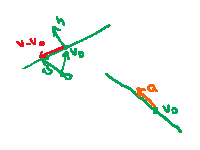
\includegraphics[height=4cm]{lecture26_drawing_1}
    \vspace{-110pt}
\end{wrapfigure}

Способы задания:
\begin{enumerate}
    \item $Ax + By = 0 \quad\quad (A, B) \neq (0, 0)$ --- нормаль.
    \item векторное уравнение $(v - v_0, n) = 0$, где $n$ --- нормаль.
    \item параметрическое уравнение $v = v_0 + at$, где $a$ --- направляющий вектор.

        \begin{math}
            \begin{cases}
                x = x_0 + a_1 t, \\
                y = y_0 + a_2 t.
            \end{cases} \quad
            \begin{gathered}
                a = (a_1, a_2) \\
                v_0 = (x_0, y_0)
            \end{gathered}
        \end{math}
\end{enumerate}

\paragraph{Уравнение прямой проходящей через две различные точки $(x_0, y_0)$ и $(x_1, y_1)$}

\begin{equation*}
    \begin{vmatrix} 
        x - x_0 & y - y_0 \\
        x_1 - x_0 & y_1 - y_0
    \end{vmatrix} = 0 \hspace{1cm}
    \frac{x - x_0}{x_1 - x_0} = \frac{y - y_0}{y_1 - y_0} \hspace{1cm}
    \begin{gathered}
        x_1 = x_0 \implies x = x_0, \\
        y_1 = y_0 \implies y = y_0.
    \end{gathered}
\end{equation*}


\subsection{Плоскости в $\RR^3$: различные способы задания, уравнение плоскости, проходящей через три точки, не лежащие на одной прямой}

\begin{wrapfigure}{r}{4.5cm}
    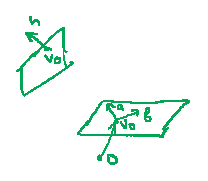
\includegraphics[width=4.5cm]{lecture26_drawing_2}
    \vspace{-30pt}
\end{wrapfigure}

Способы задания:

\begin{enumerate}
    \item $Ax + By + Cz = D \quad\quad(A, B, C) \neq (0, 0, 0)$ --- нормаль.
    \item векторное уравнение $(v - v_0, n) = 0$.
    \item параметрическое уравнение $v = v_0 + at + bs$, где $a, b$ --- направляющие векторы (базис в направляющем подпространстве).
\end{enumerate}

\paragraph{Уравнение плоскости, проходящей через 3 точки, не лежащие на одной прямой $(x_0, y_0, z_0), (x_1, y_1, z_1), (x_2, y_2, z_2)$}

\begin{equation*}
    \begin{vmatrix} 
        x - x_0 & y - y_0 & z - z_0 \\
        x_1 - x_0 & y_1 - y_0 & z_1 - z_0 \\
        x_2 - x_0 & y_2 - y_0 & z_2 - z_0
    \end{vmatrix} = 0
.\end{equation*}


\subsection{Прямые в $\RR^3$: различные способы задания, уравнение прямой, проходящей через две различные точки}

\begin{wrapfigure}{r}{3.5cm}
    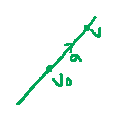
\includegraphics[width=2.5cm]{lecture26_drawing_3}
    \vspace{-30pt}
\end{wrapfigure}

Способы задания:
\begin{enumerate}
\item 
    \begin{math}
        \begin{cases}
            A_1 x + B_1 y + C_1 z = D_1, \\
            A_2 x + B_2 y + C_2 z = D_2
        \end{cases} \hspace{1cm} 
        \rk \begin{pmatrix} A_1 & B_1 & C_1 \\ A_2 & B_2 & C_2 \end{pmatrix} = 2
    \end{math}

\item векторное уравнение $[v - v_0, a] = 0$, где $v - v_0$ --- точка, $a$ --- направляющий вектор.
\item параметрическое уравнение $v = v_0 + at$. 

    \begin{math}
        \begin{gathered}
            v_0 = (x_0, y_0, z_0) \\
            a = (a_1, a_2, a_3)
        \end{gathered}
        \quad \longrightarrow \quad
        \begin{cases}
            x = x_0 + a_1 t, \\
            y = y_0 + a_2 t, \\
            z = z_0 + a_3 t.
        \end{cases}
        \quad \iff \quad
        \colorboxed{red}{\dfrac{x - x_0}{a_1} = \dfrac{y - y_0}{a_2} = \dfrac{z - z_0}{a_3}}
        \text{ --- каноническое уравнение прямой}
    \end{math}

    Если, например $a_1 = 0$, то пишут 
    \begin{math}
        \begin{cases}
            \displaystyle
            \frac{y - y_0}{a_2} = \frac{z - z_0}{a_3} \\
            x = x_0
        \end{cases}
    \end{math}
\end{enumerate}

\paragraph{Уравнение прямой, проходящей через $(x_0, y_0, z_0)$ и $(x_1, y_1, z_1)$}

\begin{equation*}
    \frac{x - x_0}{x_1 - x_0} = \frac{y - y_0}{y_1 - y_0} = \frac{z - z_0}{z_1 - z_0}
.\end{equation*}


\subsection{Взаимное расположение двух плоскостей, двух прямых, прямой и плоскости}

\subsubsection{Двух плоскостей}

\begin{wrapfigure}{r}{10cm}
    \vspace{-70pt}
    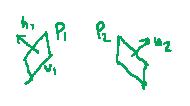
\includegraphics[width=5cm]{lecture26_drawing_4}
\end{wrapfigure}

\begin{enumerate}[nosep]
    \item \label{lec26:l1} Совпадают.
    \item \label{lec26:l2} Параллельны.
    \item Пересекаются по прямой.
\end{enumerate}

\medskip
$\hyperref[lec26:l1]{1)}, \ \hyperref[lec26:l2]{2)} \iff [u_1, u_2] = \overrightarrow{0}$.


\subsubsection{Двух прямых}

\begin{wrapfigure}{r}{10cm}
    \vspace{-70pt}
    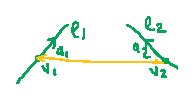
\includegraphics[width=5cm]{lecture26_drawing_5}
\end{wrapfigure}

\begin{enumerate}[nosep]
    \item \label{lec26:l3} Совпадают.
    \item \label{lec26:l4} Параллельны.
    \item \label{lec26:l5} Пересекаются в точке.
    \item Скрещиваются.
\end{enumerate}

\medskip
$\hyperref[lec26:l3]{1)}, \ \hyperref[lec26:l4]{2)} \iff [a_1, a_2] = \overrightarrow{0}$.

$\hyperref[lec26:l3]{1)}, \ \hyperref[lec26:l4]{2)}, \ \hyperref[lec26:l5]{3)} \iff (a_1, a_2, v_1 - v_2) = 0$.


\subsubsection{Прямой и плоскости}

\begin{wrapfigure}{r}{10cm}
    \vspace{-20pt}
    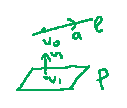
\includegraphics[height=2cm]{lecture26_drawing_6}
    \vspace{-110pt}
\end{wrapfigure}

Пусть $l$ --- прямая, $P$ --- плоскость.

\begin{enumerate}[nosep]
    \item \label{lec26:l6} $l \subseteq P$.
    \item \label{lec26:l7} $l \parallel P$.
    \item Пересекаются в точке.
\end{enumerate}

\medskip
$\hyperref[lec26:l6]{1)}, \ \hyperref[lec26:l7]{2)} \iff (a, n) = 0$.

    \section{Лекция 11.04.2020} 

Если у вас ощущение, что в конспекте баг, можете проверить \href{https://www.dropbox.com/s/xsc0pnkmmre2yhe/LA_19-20_osn_Lecture27.svg?dl=0}{снимок доски}, \href{https://youtube.com/watch?v=6WN92vn1HMQ&list=PLEwK9wdS5g0oP4vhnGvQHPSqshML3Ze4P&index=4&t=0s}{запись} и \href{https://www.dropbox.com/s/wnao00nkxnvb9h3/LO_basics.pdf?dl=0}{слайды}.

\subsection{Метрические задачи в $\RR^3$}

\subsubsection{Расстояния от точки $v$ до прямой $l = v_0 + at$}

{
\begin{wrapfigure}[1]{r}{4cm}
    \vspace{-40pt}
    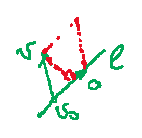
\includegraphics[height=2.5cm]{lecture27_drawing_1}
\end{wrapfigure}

\begin{equation*}
    \displaystyle
    \rho(v, l) = \frac{\left|[v - v_0, a]\right|}{|a|}
\end{equation*}
}


\subsubsection{Расстояние от точки $v$ до плоскости $P$ с направляющей нормалью $n$ и направляющим подпространством $S$ ($S = n^{\perp}$)}

{
\begin{wrapfigure}{r}{4cm}
    \vspace{-20pt}
    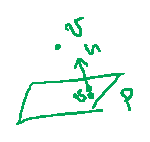
\includegraphics[height=2.5cm]{lecture27_drawing_2}
\end{wrapfigure}

\begin{equation*}
    \displaystyle
    \rho(v, P) = \left|\ort_S (v - v_0)\right| = \left|\pr_{\left< n \right>} (v - v_0)\right| = \left|\frac{(v - v_0, n)}{(n, n)} n\right| = \frac{|(v - v_0, n)|}{|n|}.
\end{equation*}
\vspace{1cm}
}


\subsubsection{Расстояние между двумя скрещивающимися прямыми $l_1 = v_1 + a_1 t$ и $l_2 = v_2 + a_2 t$}

{
\begin{wrapfigure}{r}{4.5cm}
    \vspace{-10pt}
    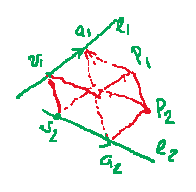
\includegraphics[height=3.5cm]{lecture27_drawing_3}
\end{wrapfigure}

\begin{equation*}
    \begin{gathered}
        p_1 = v_1 + \left< a_1, a_2 \right> \\
        p_2 = v_2 + \left< a_1, a_2 \right> \\
        \rho(l_1, l_2) = \rho(p_1, p_2)
    \end{gathered}
    \hspace{2cm}
    \rho(l_1, l_2) = \frac{\left|(a_1, a_2, v_1 - v_2)\right|}{\left|[a_1, a_2]\right|}
\end{equation*}
\vspace{1.5cm}
}


\subsubsection{Угол между прямой $l$ с направляющим вектором $a$ и плоскостью $P$ с нормалью $n$}

{
\begin{wrapfigure}{r}{6cm}
    \vspace{-10pt}
    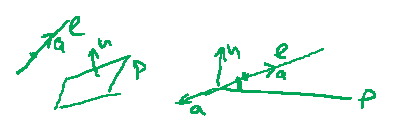
\includegraphics[height=2cm]{lecture27_drawing_4}
\end{wrapfigure}

\begin{equation*}
    \angle(l, P) = \frac{\pi}{2} - \min\left(\angle(a, n), \angle(a, -n)\right)
\end{equation*}
\vspace{0.5cm}
}


\subsubsection{Угол между двумя прямыми $l_1$ с направляющим вектором $a_1$ и $l_2$ с направляющим вектором $a_2$}

{
\begin{wrapfigure}{r}{5cm}
    \vspace{-10pt}
    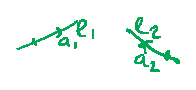
\includegraphics[height=1.5cm]{lecture27_drawing_5}
\end{wrapfigure}

\begin{equation*}
    \angle (l_1, l_2) = \min(\angle(a_1, a_2), \angle(a_1, -a_2))
.\end{equation*}
}

\subsubsection{Угол между двумя плоскостями $P_1$ с нормалью $n_1$ и $P_2$ с нормалью $n_2$}

{
\begin{wrapfigure}{r}{4cm}
    \vspace{-10pt}
    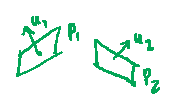
\includegraphics[height=1.5cm]{lecture27_drawing_6}
\end{wrapfigure}

\begin{equation*}
    \angle(P_1, P_2) = \min (\angle(n_1, n_2), \angle(n_1, -n_2))
.\end{equation*}
}


\subsection{Линейные операторы}

Пусть $V$ --- векторное пространство над $F$, $\dim V = n$.

\begin{definition}
\textit{Линейным оператором} (или \textit{линейным преобразованием}) на/в $V$ называется всякое линейное отображение $\phi \colon V \to V$ (то есть из $V$ \underline{\underline{в себя}}).
\end{definition}

$\L(V) := \hom(V, V)$ --- все линейные операторы на/в $V$.


\subsection{Матрица линейного оператора в фиксированном базисе}

Пусть $\phi \in \L(V)$, $\E = (e_1, \dots, e_n)$ --- базис $V$.

Тогда, $(\phi(e_1), \dots, \phi(e_n)) = (e_1, \dots, e_n) \cdot A$, $\quad A \in M_{n}(F)$.

$A$ называется матрицей линейного оператора в базисе $\E$.

Обозначение: $A(\phi, \E)$.

В столбце $A^{(j)}$ записаны координаты вектора $\phi(e_j)$ в базисе $\E$.


\subsection{Примеры линейных операторов}

\begin{enumerate}
    \item (скалярный оператор) $\lambda \in F \leadsto \phi = \lambda \cdot \mathrm{Id}$.

        $\phi(v) = \lambda \cdot v$ для всех $v \in V$.

        Для любого базиса $\E$ имеем $A(\phi, \E) = \lambda \cdot E$.

    \item $V = \RR^2$, $\phi$ --- поворот на угол $\alpha$ (вокруг 0)

        $\E = (e_1, e_2)$ положительно ориентированный ортонормированный базис $\implies A(\phi, \E) = \begin{pmatrix} 
            \cos \alpha & -\sin \alpha \\
            \sin \alpha & \cos \alpha
        \end{pmatrix}$.

    \item $V = F[x]_{\leq n}$, $\phi \colon f \mapsto f'$ (отображение дифференцирования)

        (при $F \neq \RR$ полагают по определению $x^k \mapsto kx^{k - 1}$, $k = 0, \dots, n$)

        Если $\E = (1, x, x^2, \dots, x^{n})$, то $A(\phi, \E) = \begin{pmatrix} 
            0 & 1 & 0 & 0 & \dots & 0 \\
            0 & 0 & 2 & 0 & \dots & 0 \\
            0 & 0 & 0 & 3 & \dots & 0 \\
            \vdots & \vdots & \vdots & \vdots & \ddots & \vdots \\
            0 & 0 & 0 & 0 & \dots & n \\
            0 & 0 & 0 & 0 & \dots & n
        \end{pmatrix}$.
\end{enumerate}


\subsection{Следствия общих фактов о линейных отображениях}

\begin{enumerate}
    \item $\E$ --- базис $V \implies $ отображение $\L(V) \to M_n(F)$, $\phi \mapsto A(\phi, \E)$, является изоморфизмом векторных пространств. В частности:
        \begin{enumerate}[label=\alph*)]
        \item $\phi$ однозначно определяется своей матрицей в любом базисе.
        \item Если $\E$ --- фиксированный базис $V$, то $\forall A \in M_n(F) \ \exists! \phi \in \L(V) : A(\phi, \E) = A$.
        \end{enumerate}

    \item
        $\phi \in \L(V)$, $\E = (e_1, \dots, e_n)$ --- базис $V$, $A = A(\phi, \E)$, 

        \begin{math}
            \begin{cases}
                v = x_1 e_1 + \dots + x_n e_n \\
                \phi(v) = y_1 e_1 + \dots + y_n e_n
            \end{cases} \implies \begin{pmatrix} y_1 \\ \dots \\ y_n \end{pmatrix} = A \cdot \begin{pmatrix} x_1 \\ \dots \\ x_n \end{pmatrix}
        \end{math}

    \item $\E'$ --- другой базис $V$, $\E' = \E \cdot C$, $C \in M_n^{0}(F)$

        $A = A(\phi, \E)$, $A' = A(\phi, \E') \implies A' = C^{-1} A C$.
\end{enumerate}

Следствия из 3:
\begin{enumerate}[label=\alph*)]
    \item $\det A$ не зависит от выбора базиса $\left(\det (C^{-1} A C) = \det A\right)$.
    \item $\tr A$ не зависит от выбора базиса $\left(\tr (C^{-1} A C) = \tr (ACC^{-1}) = \tr A\right)$.
\end{enumerate}


\subsection{Инвариантность определителя и следа матрицы линейного оператора относительно замены базиса}

\begin{comment}
    $\det A$ и $\tr A$ являются инвариантами самого линейного оператора $\phi$.

    Обозначаются: $\det \phi$, $\tr \phi$.
\end{comment}


\subsection{Подобные матрицы, отношение подобия на множестве квадратных матриц фиксированного порядка}

\begin{definition}
    Матрицы $A, A' \in M_n$ называются \textit{подобными}, если $\exists C \in M_n^{0}(F)$, такая что $A' = C^{-1} A C$.
\end{definition}

\begin{comment}
    Отношение подобия является отношением эквивалентности на $M_n(F)$.

    $M_n(F)$ разбивается на классы подобных матриц.
\end{comment}


\subsection{Критерий обратимости линейного оператора в терминах его ядра, образа и определителя}

Пусть $\phi \in \L(V)$.

\begin{proposal}
    Следующие условия эквивалентны:
    \begin{enumerate}[nosep]
    \item $\ker \phi = \{0\}$.
    \item $\Im \phi = V$.
    \item $\phi$ обратима (то есть $\phi$ --- изоморфизм $V$ на себя).
    \item $\det \phi \neq 0$.
    \end{enumerate}
\end{proposal}

\begin{proof}~
    \begin{description}
        \item[$1) \iff 2)$] так как $\dim V = \dim \ker \phi + \dim \Im \phi$. 
        \item[$1) \& 2) \iff 3)$]
        \item[$2) \iff 4)$] $\Im \phi = V \iff \rk \phi = \dim V \iff \det \phi = 0$.
    \end{description}
\end{proof}

\begin{definition}
    Линейный оператор $\phi \in \L(V)$ называется 
    \begin{math}
        \begin{gathered}[t]
            \textit{вырожденным}, \text{ если } \det \phi = 0, \\
            \textit{невырожденным}, \text{ если } \det \phi \neq 0.    
        \end{gathered}
    \end{math}
\end{definition}


\subsection{Подпространства, инвариантные относительно линейного оператора}

\begin{definition}
    Подпространство $U \subseteq V$ называется \textit{инвариантным относительно $\phi$} (или $\phi$-\textit{инвариантным}), \\если $\phi(U) \subseteq U$ (то есть $\phi(u) \in U \ \forall u \in U$).    
\end{definition}

В этой ситуации корректно определён линейный оператор $\phi\Big|_U \colon U \to U$, $u \mapsto \phi(u)$ называется \textit{ограничением} $\phi$ на инвариантное подпространство $U$.


\subsection{Примеры}

\begin{enumerate}
\item Подпространства $\{0\}$ и $V$ всегда $\phi$-инвариантны.
\item $\ker \phi$ --- $\phi$-инвариантно, так как $\phi(\ker \phi) = \{0\} \subseteq \ker \phi$.
\item $\Im \phi$ --- $\phi$-инвариантно, так как $\phi(\Im \phi) \subseteq \phi(V) = \Im \phi$.
\end{enumerate}



\subsection{Наблюдения}

Пусть $\phi \in \L(V)$.

\begin{enumerate}
    \item 
        Пусть $U \subseteq V$ --- $\phi$-инвариантное подпространство, $(e_1, \dots, e_k)$ --- базис $U$, дополним его до базиса $(e_1, \dots, e_n)$ всего $V$.
        
        Тогда $A(\phi, \E)$ имеет вид
        \begin{equation}
            \label{lec27:mat}
            \kbordermatrix{
                  & k & n - k \\
                k & A & B \\
                n - k & 0 & C
            }
        .\end{equation}

        При этом $A\left(\phi\big|_U, (e_1, \dots, e_k)\right) = A$.

        Если
        \begin{math}
            \begin{aligned}[t]
                &U = \ker \phi \implies A = 0, \\
                &U = \Im \phi \implies C = 0.
            \end{aligned}
        \end{math}

        Обратно, если для некоторого базиса $\E = (e_1, \dots, e_k) \quad A(\phi, \E)$ имеет вид $\eqref{lec27:mat}$, то векторы $e_1, \dots, e_k$ порождают $\phi$-инвариантное подпространство.

    \item
        Аналогично: $e_{k + 1}, \dots, e_n$ порождают $\phi$-инвариантное подпространство $\iff A(\phi, \E)$ имеет вид
        \begin{equation*}
            \kbordermatrix{
                  & k & n - k \\
                k & A & 0 \\
                n - k & B & C
            }
        .\end{equation*}

    \item 
        Пусть $U_1, U_2 \subseteq V$ --- два $\phi$-инвариантных подпространства, такие что $V = U_1 \oplus U_2$.
        
        Пусть $(e_1, \dots, e_k)$ --- базис $U_1$, $(e_{k + 1}, \dots, e_n)$ --- базис $U_2$.
        Тогда, $\E = (e_1, \dots, e_n)$ --- базис $V$ и $A(\phi, \E)$ имеет вид
        \begin{equation*}
            \kbordermatrix{
                      & k & n - k \\
                k     & \star & 0 \\
                n - k & 0 & \diamond
            }
        .\end{equation*}

    \item
        $A(\phi, \E)$ имеет блочно-диагональный вид
        \begin{center}
            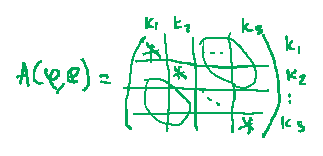
\includegraphics{lecture27_drawing_7}
        \end{center}

        Тогда и только тогда, когда подпространства $U_1, \dots, U_s \ \phi$-инвариантны, где 
        \begin{math}
            \begin{aligned}[t]
                U_1 &= \left<e_1, \dots e_{k_1}\right> \\
                U_2 &= \left< e_{k_1 + 1}, \dots, e_{k_2} \right> \\
                    &\vdots \\
                U_s &= \left< e_{n - k_s + 1}, \dots, e_n \right>
            \end{aligned}
        \end{math}

        Предел мечтаний: найти такой базис $\E$, что $A(\phi, \E)$ диагональна.

        К сожалению, это не всегда возможно.
        \hspace{0.3cm}\raisebox{-0.3cm}{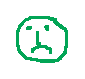
\includegraphics{lecture27_drawing_8}}
\end{enumerate}

    \section{Лекция 19.04.2018}

$V$ --  векторное пространство над полем $F$

$dim V = n$

$\varphi \in L(V)$

\subsection{Наблюдения}

4) $A(\varphi, e) = \left(
\begin{array}{c|c|c|c|c}
  * & 0 & 0 & \dots & 0  \\
  \hline
  0 & * & 0 & \dots & 0  \\
  \hline
  0 & 0 & * & \dots & 0 \\
  \hline
  \vdots & \vdots & \vdots & \vdots & \vdots \\
  \hline
  0 & 0 & 0 & \dots & * \\
\end{array}
\right)$ -- блочно-диагональный вид (каждая звездочка размера $k_i \times k_i$ для $i \in 1, \dots, s$) $\Leftrightarrow$ все подпространства $U_1, \dots, U_s$ $\varphi$-инвариантны, где $U_1 = <e_1, \dots, e_{k_1}>, U_2 = <e_{k_1 + 1}, \dots, e_{k_1 + k_2}>, \dots, U_s = <e_{n-k_s+1}, \dots, e_n>$. При этом $V = U_1 \oplus \dots \oplus U_s$.

Предел мечтаний: найти такой базис $e$, в котором $A(\varphi, e)$ диагональна (увы, это не всегда возможно).

\vspace{\baselineskip}
\textbf{Определение.} Вектор $v \in V$ называется \textit{собственным вектором} линейного оператора $\varphi$, если $v \neq 0$ и $\varphi(v) = \lambda v$ для некотрого $\lambda$. 

\vspace{\baselineskip}
\textbf{Определение.} Элемент $\lambda \in F$ называется \textit{собственным значением} линейного оператора $\varphi$, если $\exists v \in V$, такой что $v \neq 0$ и $\varphi(v) = \lambda v$.

\vspace{\baselineskip}
\textbf{Определение.} Множество собственных значений линейного оператора $\varphi$ называется его \textit{спектром}.

Обозначение: $Spec(\varphi)$

\vspace{\baselineskip}
\textbf{Замечание.} В ситуации $\varphi(v) = \lambda v, \ v \neq 0$, говорят:

1) $v$ -- собственный вектор, отвечающий собственному значению $\lambda$

2) $\lambda$ -- собственное значение, отвечающее собственному вектору $v$

\vspace{\baselineskip}
\textbf{Предложение.} $0 \neq v \in V$ является собственным для линейного оператора $\varphi \Leftrightarrow <v>$ -- $\varphi$-инвариантное подпространство.

\vspace{\baselineskip}
\textbf{\textit{Доказательство.}} $\rhd \ (\Rightarrow) \varphi(v) = \lambda v \Rightarrow w \in <v> \Rightarrow w = \mu v, \mu in F$

$\varphi(w) = \varphi(\mu v) = \mu \varphi(v) = \mu \lambda v \in <v>$

$(\Leftarrow)$ Имеем $\varphi(v) \in <v> \Rightarrow \varphi(v) = \lambda v$ для некоторого $\lambda in F \ \lhd$

\vspace{\baselineskip}
Примеры.

1) $\varphi = \lambda \cdot Id$ -- скалярный оператор

$\varphi(v) = \lambda v \ \forall \ v \in V$

$\forall \ v \in V$ являются собственными с собственным значением $\lambda$

2) $V = \RR^2, \ \varphi$ -- ортогональная проекция на прямую $l$, проходящую через 0

$v \in l \setminus \{0\} \Rightarrow \varphi(v) = v \Rightarrow v$ -- собственный вектор с собственным значением 1

$v \in l^{\bot} \setminus \{0\} \Rightarrow \varphi(v) = 0 \Rightarrow v$ -- собственный вектор с собственным значением 0

3) $\varphi: \RR^2 \rightarrow \RR^2$ -- поворот на угол $\alpha \neq \pi k$ ($\alpha = 2 \pi k \Rightarrow \varphi = Id$, $\alpha = \pi + 2 \pi k \Rightarrow \varphi = Id$)

Собственных векторов нет

4) $V = F[x]_{\leq n}$

$\varphi: f \rightarrow f'$ -- дифференцирование

$f$ -- собственный вектор $\Leftrightarrow f = const$

собственное значение 0

\vspace{\baselineskip}
\textbf{Определение.} Линейный оператор $\varphi$ называется \textit{диагонализуемым}, если $\exists$ базис $e$ пространства $V$, такой что матрица $A(\varphi, e)$ диагональна.

\vspace{\baselineskip}
\textbf{Предложение.} Линейный оператор $\varphi$ диагонализуем $\Leftrightarrow$ в $V \ \exists$ базис, состоящий из собственных векторов для $\varphi$.

\vspace{\baselineskip}
\textbf{\textit{Доказательство.}} $\rhd \ e = (e_1, \dots, e_n)$ -- базис $V \Rightarrow A(\varphi, e) = diag(\lambda_1, \dots, \lambda_n) = \begin{pmatrix} \lambda_1 & 0 & \dots & 0 \\ 0 & \lambda_2 & \dots & 0 \\ \vdots & \vdots & \vdots & \vdots \\ \ 0 & 0 & \dots & \lambda_n \end{pmatrix} \Leftrightarrow \varphi(e_1) = \lambda_1 e_1, \dots, \varphi(e_n) = \lambda_n e_n \Leftrightarrow e_1, \dots, e_n$ -- собственные векторы

\vspace{\baselineskip}
Примеры выше.

1) $\varphi$ уже диагонализован, т.к. $\forall$ вектор $\neq 0$ является собственным

2) $e_1 \in l, e_2 \in l^{\bot} \Rightarrow (e_1, e_2)$ -- базис из собственных векторов $\Rightarrow \varphi$ диагонализуем

$A(\varphi, e) = \begin{pmatrix} 1 & 0 \\ 0 & 0 \end{pmatrix}$

3) не диагонализуем, т.к. нет собственных векторов

4) $\varphi$ диагонализуем $\Rightarrow n = 0$

\vspace{\baselineskip}
$\varphi \in L(V), \lambda \in F$

$V_{\lambda} (\varphi) := \{v \in V \ | \ \varphi(v) = \lambda v \}$

\vspace{\baselineskip}
\textbf{\textit{Упражнение.}} $V_{\lambda} (\varphi)$ -- подпространство в $V$

\vspace{\baselineskip}
\textbf{\textit{Лемма.}} $V_{\lambda} (\varphi) \neq 0 \Leftrightarrow \lambda \in Spec(\varphi)$

\vspace{\baselineskip}
\textbf{\textit{Доказательство.}} Следует из определения.

\vspace{\baselineskip}
\textbf{Определение.} $\lambda \in Spec(\varphi) \Rightarrow V_{\lambda} (\varphi)$ называется \textit{собственным подпространством}, отвечающим собственному значению $\lambda$.

\vspace{\baselineskip}
\textbf{Замечание.} $V_{\lambda} (\varphi)$ -- $\varphi$-инвариантное подпространство

$\varphi |_{V_{\lambda} (\varphi)} = \lambda \cdot Id |_{V_{\lambda} (\varphi)}$

\vspace{\baselineskip}
\textbf{Предложение.} $\lambda \in F \Rightarrow V_{\lambda} (\varphi) = Ker(\varphi - \lambda \cdot Id)$

\vspace{\baselineskip}
\textbf{\textit{Доказательство.}} $\rhd \ v \in V_{\lambda} (\varphi) \Leftrightarrow \varphi (v) = \lambda v \Leftrightarrow \varphi(v) - \lambda v = 0 \Leftrightarrow (\varphi - \lambda \cdot Id) v = 0 \Leftrightarrow v \in Ker(\varphi - \lambda \cdot Id) \ \lhd$

\vspace{\baselineskip}
\textbf{Следствие.} $\lambda \in Spec(\varphi) \Leftrightarrow det(\varphi - \lambda \cdot Id) = 0$

\vspace{\baselineskip}
\textbf{\textit{Доказательство.}} $\rhd \ \lambda \in Spec(\varphi) \Leftrightarrow V_{\lambda} (\varphi) \neq \{0\} \Leftrightarrow Ker(\varphi - \lambda \cdot Id) \neq 0 \Leftrightarrow det (\varphi - \lambda \cdot Id) = 0 \ \lhd$

\vspace{\baselineskip}
\textbf{Определение.} Многочлен $\chi_{\varphi} (t) = (-1)^n det (\varphi - t \cdot Id)$ называется $\textit{характеристическим многочленом}$ линейного оператора $\varphi$.

\vspace{\baselineskip}
Если $e$ -- какой-либо базис $V$, $A = (a_{ij}) = A(\varphi, e)$, то

$\chi_{\varphi} (t) = (-1)^n det (A - t \cdot E) = (-1)^n \begin{vmatrix} a_{11} - t & a_{12} & a_{13} & \dots & a_{1n} \\
a_{21} & a_{22} - t & a_{23} & \dots & a_{2n} \\ 
a_{31} & a_{32} & a_{33} - t & \dots & a_{3n} \\
\vdots & \vdots & \vdots & \vdots & \vdots \\
a_{n1} & a_{n2} & a{n3} & \dots & a_{nn} - t \end{vmatrix}$

\vspace{\baselineskip}
$\chi_{\varphi} (t) = t^n + c_{n-1} t^{n-1} + \dots + c_1 t + c_0, \ c_0 = (-1)^n det \varphi, \ c_{n-1} = -tr \varphi$

\vspace{\baselineskip}
Вывод из разобранного выше:

\textbf{Утверждение.} $\lambda \in Spec(\varphi) \Leftrightarrow \chi_{\varphi} (\lambda) = 0$, т.е. $\lambda$ -- корень характеристического многочлена

\vspace{\baselineskip}
\textbf{Следствие.} $|Spec(\varphi)| \leq n$

\vspace{\baselineskip}
\textbf{Следствие.} $F = \CC \Rightarrow \forall \ \varphi \in L(V) \ \exists$ собственный вектор

\vspace{\baselineskip}
\textbf{\textit{Доказательство.}} $\rhd \ \chi_{\varphi} (t)$ имеет корень по основной теореме алгебры комплексных чисел $\lhd$

\vspace{\baselineskip}
$\lambda \in Spec(\varphi)$

$k_\lambda$ -- кратность $\lambda$ как корня многочлена $\chi_{\varphi} (t)$, т.е. $\chi_{\varphi} (t)$ делится на $(t - \lambda)^{k_{\lambda}}$, но не делится на большую степень

\vspace{\baselineskip}
\textbf{Определение.} Число $k_{\lambda}$ называется \textit{алгебраической кратностью} собственного значения $\lambda$.

\vspace{\baselineskip}
\textbf{Определение.} Число $dim V_{\lambda} (\varphi)$ называется $\textit{геометрической кратностью}$ собственного значения $\lambda$.

\vspace{\baselineskip}
\textbf{Предложение.} $\lambda \in Spec(\varphi) \Rightarrow$ (геометрическая кратность $\lambda$) $\leq$ (алгебраическая кратность $\lambda$)

\vspace{\baselineskip}
\textbf{\textit{Доказательство.}} $\rhd$ Положим $m_{\lambda} = dim V_{\lambda} (\varphi)$, т.е. $m_{\lambda}$ -- геометрическая кратность для $\lambda$. Пусть $(e_1, \dots, e_{m_\lambda})$ -- базис $V_{\lambda} (\varphi)$. Дополним его до базиса $e = (e_1, \dots, e_n)$ всего $V$.

Тогда $A(\varphi, e) = \left( \begin{array}{c|c}
  A & B  \\
  \hline
  0 & D  \\
\end{array}
\right), A = \begin{pmatrix} \lambda & 0 & \dots & 0 \\ 0 & \lambda & \dots & 0 \\ \vdots & \vdots & \vdots & \vdots \\ 0 & 0 & \dots & \lambda \end{pmatrix} \in M_{m_{\lambda}}, B \in Mat_{m_{\lambda} \times (n - m_{\lambda})}, D \in M_{n - m_{\lambda}} \Rightarrow$

$\chi_{\varphi}(t) = (-1)^n \left| \begin{array}{c|c}
  A - t \cdot E & B  \\
  \hline
  0 & D - t \cdot E  \\
\end{array}
\right|  = (-1)^n (\lambda - t)^{m_\lambda} \cdot det (D - t \cdot E) = (t - \lambda)^{m_\lambda} \cdot (-1)^{n - m_{\lambda}} \cdot det (D - t \cdot E) \Rightarrow \chi_{\varphi} (t) \vdots (t - \lambda)^{m_{\lambda}} \Rightarrow$

(алгебраическая кратность $\lambda$) $\geq m_{\lambda} \ \lhd$


    \section{Лекция 23.04.2020} 

Конспект полностью написан по
\href{https://www.dropbox.com/s/ze7leityir3zbqo/LA_19-20_osn_Lecture29.svg?dl=0}{снимку доски}, 
\href{https://www.youtube.com/watch?v=_J8hatdsSrM}{записи лекции} и
\href{https://www.dropbox.com/s/as7uz9v74ba9u5f/LinOperators2.pdf?dl=0}{слайдам},
возможны баги при переписывании. Если хочется понять точно ли что-то правда, лучше смотреть туда.


\subsection{Критерий диагонализуемости линейного оператора в терминах его характеристического многочлена, а также алгебраической и геометрической кратностей его собственных значений}

Пусть $V$ --- векторное пространство над $F$, $\dim V = n$, $\phi \in \L(V)$ --- линейный оператор.

\begin{theorem}{(критерий диагонализуемости)}
    $\phi$ диагонализуемо $\iff$ выполняются одновременно следующие 2 условия:
    \begin{enumerate}
    \item $\chi_\phi(t)$ разлагается на линейные множители.
    \item $\forall \lambda \in \spec \phi \quad g_\lambda = a_\lambda$.
    \end{enumerate}
\end{theorem}

\begin{proof}~
    \begin{description}
    \item[$\implies$] $\phi$ диагонализуемо $\implies \exists$ базис $\E = (e_1, \dots, e_n)$, такой что $\chi_\phi(t)$ разлагается на линейные множители:
        \begin{equation*}
            A(\phi, \E) = \begin{pmatrix} 
                \mu_1 & 0 & \dots & 0 \\
                0 & \mu_2 & \dots & 0 \\
                \vdots & \vdots & \ddots & \vdots \\
                0 & 0 & \dots & \mu_n
            \end{pmatrix} \implies \chi_\phi(t) = (-1)^n \begin{vmatrix} 
                \mu_1 - t & 0 & \dots & 0 \\
                0 & \mu_2 - t & \dots & 0 \\
                \vdots & \vdots & \ddots & \vdots \\
                0 & 0 & \dots & \mu_n - t
            \end{vmatrix} = (t - \mu_1) \cdot \ldots \cdot (t - \mu_n)
        .\end{equation*}

        Перепишем $\chi_\phi(t)$ в виде $\chi_\phi(t) = (t - \lambda_1)^{k_1} \cdot \ldots \cdot (t - \lambda_s)^{k_s}$, где $ \{\mu_1, \dots, \mu_n\} = \{\lambda_1, \dots, \lambda_s\}, \quad \lambda_i \neq \lambda_j$ при $i \neq j$.

        $\forall i = 1, \dots, s$ имеем $V_{\lambda_i}(\phi) \supseteq \left< e_j \mid \mu_j = \lambda_i \right> \implies \dim V_{\lambda_i}(\phi) \geq k_i$, то есть $g_{\lambda_i} \geq a_{\lambda_i}$.

        Но мы знаем, что $g_{\lambda_i} \leq a_{\lambda_i}$. Следовательно, $a_{\lambda_i} = g_{\lambda_i}$.

    \item[$\impliedby$] Пусть $\chi_\phi(t) = (t - \lambda_1)^{k_1} \cdot \ldots \cdot (t - \lambda_s)^{k_s}$, $\lambda_i \neq \lambda_j$ при $i \neq j$.

        Так как подпространства $V_{\lambda_1}(\phi), \dots, V_{\lambda_s}(\phi)$ линейно независимы, то 
        \begin{equation*}
            \dim(V_{\lambda_1}(\phi) + \dots + V_{\lambda_s}(\phi)) = \dim V_{\lambda_1}(\phi) + \dots + \dim V_{\lambda_s}(\phi) = k_1 + \dots + k_s = n = \dim V
        .\end{equation*}
        Следовательно, $V = V_{\lambda_1}(\phi) \oplus \dots \oplus V_{\lambda_s}(\phi)$.

        Если $\E_i$ --- базис в $V_{\lambda_i}(\phi)$, то $\E = \E_1 \sqcup \dots \sqcup \E_s$ --- базис всего $V$, состоящий из собственных векторов, а значит $\phi$ диагонализуем.
        \qedhere
    \end{description}
\end{proof}

\paragraph{Примеры}

\begin{enumerate}
    \item $\phi = \lambda \cdot \mathrm{Id}$ --- скалярный оператор.

        Для всякого базиса $\E$ в $V$ имеем $A(\phi, \E) = \diag(\lambda, \dots, \lambda)$.

        $\chi_\phi(t) = (t - \lambda)^n$.

        $\spec \phi = \{\lambda\}$, $a_\lambda = n = g_\lambda \implies $ условия 1) и 2) выполнены.

    \item $V = \RR^2$, $\phi$ --- ортогональная проекция на прямую $l \ni 0$.

        $e_1 \in l \setminus \{0\}$, $e_2 \in l^{\perp} \setminus \{0\}$, $\E = (e_1, e_2) \implies A(\phi, \E) = \begin{pmatrix} 1 & 0 \\ 0 & 0 \end{pmatrix}$

        $\chi_\phi(t) = t(t - 1) \implies \spec \phi = \{0, 1\}$.

        $\lambda = 0, 1 \implies a_\lambda = 1 = g_\lambda \implies $ условия 1) и 2) выполнены.

    \item $V = \RR^2$, $\phi$ --- поворот на угол $\alpha \neq \pi k$.

        $\E = (e_1, e_2)$ --- положительно ориентированный базис $\implies A(\phi, \E) = \begin{pmatrix} \cos \alpha & - \sin \alpha \\ \sin \alpha & \cos \alpha \end{pmatrix}$.

        $\chi_\phi(t) = \begin{vmatrix} \cos \alpha - t & - \sin \alpha \\ \sin a & \cos \alpha - t \end{vmatrix} = t^2 - 2 \cos \alpha \cdot t + 1$.

        $\frac{D}{4} = \cos ^2 \alpha - 1 = - \sin ^2 a < 0 \implies $ нет корней в $\RR \implies \chi_\phi(t)$ не разлагается на линейные множители над $\RR \implies $ 1) не выполнено $ \implies \phi$ не диагонализуем над $\RR$.

        Однако $\phi$ диагонализуем над $\CC$!

    \item $V = F[x]_{\leq n}$, $n \geq 1$; $\quad \phi \colon f \mapsto f'$.

        Техническое условие: $\mathop{\mathrm{char}} F = 0$ ($\iff \mathop{\mathrm{ord}} 1 = \infty$ в группе $(F, +)$), например, $F = \QQ, \RR, \CC$ подходят.

        \begin{math}
            \E = (1, x, \dots, x^n) \implies A(\phi, \E) = \begin{pmatrix}
                0 & 1 & 0 & \dots & 0 \\
                0 & 0 & 2 & \dots & 0 \\
                \vdots & \vdots & \vdots & \ddots & \vdots \\
                0 & 0 & 0 & \dots & n \\
                0 & 0 & 0 & \dots & 0
            \end{pmatrix}
        \end{math}

        $\chi_\phi(t) = t^{n + 1} \implies \spec \phi = \{0\} \implies $ 1) выполнено.

        $\lambda = 0 \implies a_\lambda = n + 1; \quad V_\lambda(\phi) = \left< 1 \right> \implies g_\lambda = 1 < a_\lambda \implies $ 2) не выполнено $\implies \phi$ не диагонализуем.

        \begin{math}
            \E' = \left(1, x, \frac{x^2}{2}, \dots, \frac{x^n}{n!}\right) \implies A(\phi, \E') = \begin{pmatrix} 
                0 & 1 & 0 & \dots & 0 \\
                0 & 0 & 0 & \dots & 0 \\
                \vdots & \vdots & \vdots & \ddots & \vdots \\
                0 & 0 & 0 & \dots & 1 \\
                0 & 0 & 0 & \dots & 0
            \end{pmatrix} = J_0^{n + 1} \text{ --- это жорданова клетка}
        \end{math}
\end{enumerate}


\subsection{Существование одномерного или двумерного инвариантного подпространства у линейного оператора в действительном векторном пространстве}

\begin{theorem}
    $F = \RR \implies \forall \phi \in L(V) \ \exists $ либо $1$-мерное, либо $2$-мерное $\phi$-инвариантное подпространство.
\end{theorem}

\begin{proof}
    Если $\chi_\phi(t)$ имеет действительные корни, то в $V$ есть собственный вектор $ \implies $ 1-мерное $\phi$-инвариантное подпространство.

    Пусть $\chi_\phi(t)$ не имеет корней в $\RR$. Возьмем какой-нибудь комплексный корень $\lambda + i \mu$, $\mu \neq 0$.

    Фиксируем базис $\E$ в $V$ и положим $A = A(\phi, \E)$. Для $\lambda + i \mu$ у матрицы $A$ существует комплексный собственный вектор, то есть такое $u, v \in \RR^n$, что
    \begin{equation*}
        A(u + iv) = (\lambda + i \mu) (u + i v) \implies Au + iAv = \lambda u - \mu v + i (\lambda v + \mu u) \implies \begin{cases}
            Au &= \lambda u - \mu v \\
            Av &= \lambda v + \mu u
        \end{cases}
    .\end{equation*}
    
    Значит, векторы в $V$ с координатами $u, v$ порождают $\phi$-инвариантное подпространство $U \subseteq V$ размерности $ \leq 2$.
\end{proof}

\begin{exercise}
    $\dim U = 2$.
\end{exercise}


\subsection{Отображение, сопряжённое к линейному отображению между двумя евклидовыми пространствами: определение, существование и единственность. Матрица сопряжённого отображения в паре произвольных и паре ортонормированных базисов}

Пусть 
\begin{math}
    \begin{aligned}[t]
        &\EE \text{ --- евклидово пространство со скалярным произведением } (\bigcdot, \bigcdot), \quad \dim \EE = n, \\
        &\EE \text{ --- другое евклидово пространство со скалярным произведением } (\bigcdot, \bigcdot)', \quad \dim \EE' = m, \\
        &\phi \colon \EE \to \EE'.
    \end{aligned}
\end{math}

\begin{definition}
    Линейное отображение $\psi \colon \EE' \to \EE$ называется \textit{сопряженным} к $\phi$, если 
    \begin{equation*}
        \label{lec29:def}
        \tag{$\star$}
        (\phi(x), y)'  = (x, \psi(y)) \quad \forall x \in \EE, y \in \EE'
    .\end{equation*}

    Обозначение: $\phi^*$.
\end{definition}

\begin{proposal}~
    \begin{enumerate}
    \item $\psi$ существует и единственно.
    \item Если $\E$ --- базис $\EE$, $\F$ --- базис $\EE'$, 
        \begin{math}
            \begin{aligned}
                G &= G(e_1, \dots, e_n) \\
                G' &= G(f_1, \dots, f_m)
            \end{aligned}
        \end{math} и 
        \begin{math}
            \begin{aligned}
                A_\phi &= A(\phi, \E, \F) \\
                A_\psi &= (A, \psi, \F, \E),
            \end{aligned}
        \end{math} то $A_\psi = G^{-1} A_\phi^{T} G'$.

        В частности, если $\E$ и $\F$ ортонормированы, то $A_\psi = A_\phi^{T}$.
    \end{enumerate}
\end{proposal}

\begin{proof}
    $x = x_1 e_1 + \dots + x_n e_n \in \EE$, $y = y_1 f_1 + \dots + y_m f_m \in \EE'$.

    \begin{equation*}
        (\phi(x), y)' = \left(A_\phi \begin{pmatrix} x_1 \\ \dots \\ x_n \end{pmatrix} \right)^{T} \cdot G' \cdot \begin{pmatrix} y_1 \\ \dots \\ y_m \end{pmatrix} = (x_1 \dots x_n) \cdot A_\phi^{T} \cdot G' \cdot \begin{pmatrix} y_1 \\ \dots \\ y_m \end{pmatrix}
    .\end{equation*}

    \begin{equation*}
        (x, \psi(y)) = (x_1 \dots x_n) \cdot G \cdot A_\psi \cdot \begin{pmatrix} y_1 \\ \dots \\ y_m \end{pmatrix}
    .\end{equation*}

    Так как $\forall B \in \text{Mat}_{m \times n} \quad b_{ij} = \underset{i}{(0 \dots 0 \ 1 \ 0 \dots 0)} \cdot B \cdot \underset{j}{(0 \dots 0 \ 1 \ 0 \dots 0)}^{T}$, то ${\eqref{lec29:def} \iff A_{\phi}^{T} G' = G A_\psi \iff A_\psi = G^{-1} A^{T}_\phi G'}$.

    Отсюда следуют сразу оба утверждения.
\end{proof}


\subsection{Сопряжённый оператор в евклидовом пространстве}

\subsection{Самосопряжённые (симметрические) операторы}

Пусть теперь $\EE' = \EE$.

$\phi \colon \EE \to \EE$ --- линейный оператор $ \implies \exists!$ линейный оператор $\phi^{*} \colon \EE \to \EE$, такой что $(\phi(x), y) = (x, \phi^{*}(y)) \quad \forall x, y \in \EE$.

\begin{definition}
    Линейный оператор $\phi \in L(\EE)$ называется \textit{самосопряженным} (или \textit{симметричным}), если $\phi = \phi^{*}$, то есть $(\phi(x), y) = (x, \phi(y)) \quad \forall x, y \in \EE`$.
\end{definition}


\subsection{Существование собственного вектора у самосопряжённого оператора}

Если $\E$ --- ортонормированный базис в $\EE$, $A_\phi = A(\phi, \E)$, $A_{\phi^{*}} = A(\phi^{*}, \E)$, то $A_{\phi^{*}} = A_\phi^{T}$.

Следовательно, $\phi = \phi^{*} \iff A_\phi = A_\phi^{T}$.

\begin{proposal}
    Если $\phi = \phi^{*}$, то $\exists$ собственный вектор для $\phi$.
\end{proposal}

\begin{proof}
    Было: $\exists$ либо
    \begin{enumerate*}[label=\arabic*)]
    \item 1-мерное $\phi$-инвариантное подпространство, либо
    \item 2-мерное $\phi$-инвариантное подпространство.
    \end{enumerate*}

    \begin{enumerate}
    \item ок.
    \item $U \subseteq \EE$ --- $\phi$-инвариантное подпространство, $\dim U = 2$.

        Фиксируем ортонормированный базис $\E = (e_1, e_2)$. Пусть $\psi = \phi \big|_{U}$.

        Значит, $\psi = \psi^{*} \implies A(\psi, \E) = \begin{pmatrix} a & b \\ b & c \end{pmatrix}$.

        Отсюда, $\chi_\psi(t) = \begin{vmatrix} a - t & b \\ b & c - t \end{vmatrix} = t^2 - (a + c)t + ac - b^2$.

        $D = (a + c)^2 - 4(ac - b^2) = (a - c)^2 + 4b^2 \geq 0$.

        Следовательно, $\chi_\psi(t)$ имеет корни в $\RR$, то есть в $U$ есть собственный вектор для $\psi$, он же собственный вектор для $\phi$.
    \end{enumerate}
\end{proof}


\subsection{Инвариантность ортогонального дополнения к подпространству, инвариантному относительно самосопряжённого оператора}

\begin{proposal}
    $\phi = \phi^{*}$, $U \subseteq \EE$ --- $\phi$-инвариантное подпространство, тогда $U^{\perp}$ --- тоже $\phi$-инвариантное подпространство.
\end{proposal}

\begin{proof}
    $\phi(U) \subseteq U$, хотим $\phi(U^{\perp}) \subseteq U^{\perp}$. $\quad \forall x \in U^{\perp} \quad \forall y \in U \quad (\phi(x), y) = (x, \phi(y)) = 0 \implies \phi(x) \in U^{\perp}$.
\end{proof}

    \section{Лекция 10.05.2018}

Пусть теперь $E' = E, \varphi: E \rightarrow E$ -- линейный оператор $\Rightarrow \ \exists!$ линейный оператор $\varphi^*: E \rightarrow E$, такой что $(\varphi(x), y) = (x, \varphi^*(y)) \ \forall \ x, y \in E$

\bigskip
\textbf{Определение.} $\varphi^*$ называется \textit{сопряженным} к $\varphi$ линейным оператором.

\bigskip
\textbf{Определение.} Линейный оператор $\varphi$ называется \textit{самомпряженным (или симметрическим)}, если $\varphi = \varphi^*$.

\bigskip
\textbf{Замечание.} $e$ -- ортогональный базис в $E, A_{\varphi} = A(\varphi, e), A_{\varphi^*} = A(\varphi^*, e) \Rightarrow A_{\varphi^*} = (A_{\varphi})^T$

$\varphi = \varphi^* \Leftrightarrow A_{\varphi} = (A_{\varphi})^T$

\bigskip
\textbf{Предложение.} $\varphi = \varphi^*, U \subseteq E$ -- $\varphi$-инвариантное подпространство $\Rightarrow U^{\bot}$ тоже $\varphi$-инвариантное

\bigskip
\textbf{\textit{Доказательство.}} $\rhd$ Имеем $\varphi(U) \subseteq U$, хотим $\varphi(U^{\bot}) \subseteq U^{\bot}$

$\forall x \in U^{\bot}, y \in U: (\varphi(x), y) = (x, \varphi^* (y)) = (\overbrace{x}^{\in U^{\bot}}, \overbrace{\varphi(y)}^{\in U}) = 0 \ \lhd$

\bigskip
\textbf{Предложение.} $\varphi = \varphi^* \Rightarrow \exists$ собственный вектор для $\varphi$

\bigskip
\textbf{\textit{Доказательство.}} $\rhd$ Два случая: 1) $\exists$ 1-мерное $\varphi$-инвариантное подпространство

2) $\exists$ 2-мерное $\varphi$-инвариантное подпространство

\bigskip
1) Очевидно

2) Пусть $U \subseteq E$ -- 2-мерное $\varphi$-инвариантное подпространство. Положим $\psi := \varphi|_U$

Т.к. $\varphi = \varphi^*$, то $\psi = \psi^*$

Пусть $(e_1, e_2)$ -- ортонормированный базис в $U \Rightarrow A(\psi, e) = \begin{pmatrix} a & b \\ b & c \end{pmatrix}$

$\chi_{\psi} (t) = (-1)^2 \begin{vmatrix}
a- t & b \\ b & c - t \end{vmatrix} = t^2 - (a + c) t + ac - b^2$

$D = (a+c)^2 - 4 (ac - b^2) = (a-c)^2 +4b^2 \geq 0 \Rightarrow \chi_{\psi} (t)$ имеет корни в $\RR \Rightarrow \psi$ имеет собственный вектор $\Rightarrow \varphi$ имеет собственный вектор $\lhd$

\bigskip
\textbf{Теорема.} $\varphi = \varphi^* \Rightarrow \exists$ ортонормированный базис, состоящий из собственных векторов для $\varphi$. В частности, $\varphi$ диагонализуем над $\RR$, $\chi_{\varphi} (t)$ разлагается на линейные множители над $\RR$.

\bigskip
\textbf{\textit{Доказательство.}} Индукция по $n = dim E$.

$n = 1 \Rightarrow$ очевидно

Пусть доказано для $<n$, докажем для $n$.

$\exists$ собственный вектор $v$ для $\varphi$.

Положим $e_1 = \frac{v}{|v|}, |e_1| = 1$.

$U = <e_1> \Rightarrow U$ $\varphi$-инвариантно $\Rightarrow U^{\bot}$ тоже $\varphi$-инвариантно

$dim U^{\bot} = n - 1 \Rightarrow$ по предположению индукции в $U^{\bot}$  $\exists$ ортонормированный базис $(e_2, \dots, e_n)$ из собственных векторов, $e_1 \bot (e_2, \dots, e_n)$. Тогда $(e_1, \dots, e_n)$ -- искомый базис $\lhd$

\bigskip
\textbf{Следствие.} $\varphi = \varphi^*, \ \lambda, \mu \in Spec(\varphi), \lambda \neq \mu \Rightarrow E_{\lambda} (\varphi) \bot E_{\mu} (\varphi)$

\bigskip
\textbf{\textit{Доказательство.}} \textbf{Первый способ.}

Пусть $e = (e_1, \dots, e_n)$ -- ортономированный базис из собственных векторов

$(\lambda_1, \dots, \lambda_n)$ -- соответствующий набор собственных значений (т.е. $\varphi (e_i) = \lambda_i e_i$)

$v = x_1 e_1 + \dots + x_n e_n \in E$

$\varphi(v) = x_1 \lambda_1 e_1 + \dots + x_n \lambda_n e_n$. Тогда $\varphi (v) = \lambda v \Leftrightarrow v \in <e_i \ | \ \lambda_i = \lambda> \Rightarrow E_{\lambda} (\varphi) = <e_i \ | \ \lambda_i = \lambda > \Rightarrow E_{\lambda} (\varphi) \bot E_{\mu} (\varphi)$ при $\lambda \neq \mu$

\bigskip
\textbf{Второй способ.}

$\lambda \neq \mu, x \in E_{\lambda} (\varphi), y \in E_{\mu} (\varphi)$

$\lambda(x, y) = (\lambda x, y) = (\varphi(x), y) = (x, \varphi(y)) = (x, \mu y) = \mu (x, y)$

Т.к. $\lambda \neq \mu$, то $(x, y) = 0 \ \lhd$

\bigskip
\textbf{Теорема (приведение квадратичной формы к главным осям).} $Q: E \rightarrow \RR$ -- квадратичная форма $\Rightarrow \exists$ ортономированный базис $e = (e_1, \dots, e_n)$, в котором $Q$ принимает канонический вид $Q(x) = \lambda_1 x_1^2 + \dots + \lambda_n x_n^2$, причем числа $\lambda_1, \dots, \lambda_n$ определены однозначно с точностью до перестановки. \textit{Главные оси} -- это $\RR e_1, \dots, \RR e_n$.

\bigskip
\textbf{\textit{Доказательство.}} $\rhd$ Пусть $f = (f_1, \dots, f_n)$ -- какой-то ортонормированный базис, $B = B(Q, f)$.

Пусть $\varphi: E \rightarrow E$ -- линейный оператор, такой что $A(\varphi, f) = B$

Т.к. $B = B^T$ и $f$ ортонормированный, то $\varphi = \varphi^*$

$\forall \ x = x_1 f_1 + \dots + x_n f_n \in E$ имеем $Q(x) = (x_1, \dots, x_n) B \begin{pmatrix} x_1 \\ \vdots \\ x_n \end{pmatrix} = (x, \varphi(x))$

Итого: $Q(x) = (x, \varphi(x)) \ \forall \ x \in E$ (*)

\bigskip
Знаем: $\exists$ ортонормированный базис $e= (e_1, \dots, e_n)$, состоящий из собственных векторов для $\varphi \Rightarrow A(\varphi, e) = diag (\lambda_1, \dots, \lambda_n)$

Но тогда $\forall \ x = x_1 e_1 + \dots + x_n e_n \ Q(x) = (x, \varphi(x)) = (x_1, \dots, x_n) D \begin{pmatrix}
x_1 \\ \vdots \\ x_n \end{pmatrix} = \lambda_1 x_1^2 + \dots + \lambda_n x_n^2$

\bigskip
Единственность: $\lambda_1, \dots, \lambda_n$ -- это в точности собственные значения линейного оператора $\varphi$

В свою очередь, $\varphi$ однозначно определяется из условия (*) $\lhd$

\bigskip
\textbf{Следствие.} $A \in M_n(\RR), A = A^T \Rightarrow \exists$ ортогональная матрица $C \in M_n$, такая что $C^{-1} A C = C^T A C = diag(\lambda_1, \dots, \lambda_n)$, причем $\lambda_1, \dots, \lambda_n$ -- это в точности собственные значения матрицы $A$.

\bigskip
\textbf{Определение.} Линейный оператор называется \textit{ортогональным}, если $\forall \ x, y \in E: (\varphi(x), \varphi(y)) = (x, y)$ (т.е. $\varphi$ сохраняет скалярное произведение)

\bigskip
\textbf{Предложение.} Для $\varphi \in L(E)$ следуюущие условия эквивалентны:

1) $\varphi$ ортогональный

2) $|\varphi(x)| = |x| \ \forall \ x \in E$ (т.е. $\varphi$ сохраняет длину)

3) $\exists \ \varphi^{-1}$ и $\varphi^{-1} = \varphi^*$

4) $\forall$ ортонормированного базиса $e$ матрица $A(\varphi, e)$ ортогональная

5) $\forall$ ортонормированного базиса $e$ $(\varphi(e_1), \dots, \varphi(e_n))$ -- тоже ортонормированный базис

\bigskip
\textbf{\textit{Доказательство.}} $\rhd$ $1) \Rightarrow 2) \ |\varphi(x)| = \sqrt[]{(\varphi(x), \varphi(x))} = \sqrt[]{(x, x)} = |x|$

\bigskip
$2) \Rightarrow 1) \ (\varphi(x), \varphi(y)) = \frac{1}{2} (|\varphi(x) + \varphi(y)|^2 - |\varphi(x)|^2 - |\varphi(y)|^2) = \frac{1}{2} (|x+y|^2 - |x|^2 - |y|^2) = (x, y)$

\bigskip
$1) \& 2) \Rightarrow 3) \ \varphi(x) = 0 \Rightarrow |\varphi(x)| = 0 \Rightarrow |x| = 0 \Rightarrow x = 0 \Rightarrow Ker \varphi = \{0\} \Rightarrow \varphi$ невырожден (т.е. $\exists \ \varphi^{-1}$)

$(\varphi^{-1}(x), y) = (\varphi(\varphi^{-1}(x)), \varphi(y)) = (x, \varphi(y)) \Rightarrow \varphi^{-1} = \varphi^*$

\bigskip
$3) \Rightarrow 4) \ e$ -- ортонормированный базис, $A = A(\varphi, e)$

$\begin{cases} A(\varphi^*, e) = A^T \\ A(\varphi^{-1}, e) = A^{-1} \end{cases} \Rightarrow A^T = A^{-1}$

\bigskip
$4) \Rightarrow 5) \ e$ -- ортонормированный базис, $A = A(\varphi, e) \Rightarrow (\varphi(e_1), \dots, \varphi(e_n)) = (e_1, \dots, e_n) A$ (где $A$ ортогональная) $\Rightarrow (\varphi(e_1), \dots, \varphi(e_n))$ -- ортонормированный базис

\bigskip
$5) \Rightarrow 1) \ e$ -- ортонормированный базис, $x = \sum\limits_{i=1}^n x_i e_i, y = \sum\limits_{j=1}^n y_j e_j$

$(\varphi(x), \varphi(y)) = (\varphi(\sum\limits_{i=1}^n x_i e_i), \varphi(\sum\limits_{j=1}^n y_j e_j)) = \sum\limits_{i=1}^n\sum\limits_{j=1}^n x_i y_j \overbrace{(\varphi(e_i), \varphi(e_j))}^{\delta_{ij}} = \sum\limits_{i=1}^n\sum\limits_{j=1}^n x_i y_j (e_i, e_j) = (\sum\limits_{i=1}^n x_i e_i, \sum\limits_{j=1}^n y_i e_j) = (x, y) \ \lhd$


    \section{Лекция 17.05.2018}

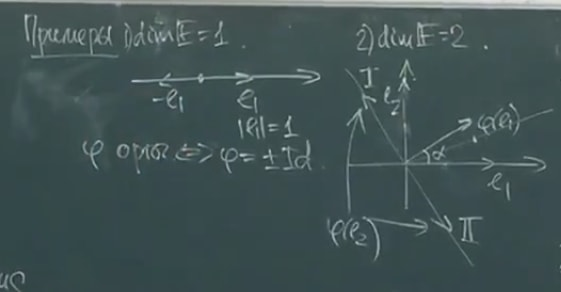
\includegraphics[width=15cm,height=12cm,keepaspectratio]{examples1.jpg}

\vspace{\baselineskip}
$(e_1, e_2)$ -- ортонормированный базис

\vspace{\baselineskip}
\RomanNumeralCaps{1} $A(\varphi, e) = \begin{pmatrix} \cos \alpha && -\sin \alpha \\ \sin \alpha && \cos \alpha
\end{pmatrix} \Rightarrow \varphi$ -- поворот на угол $\alpha$

\vspace{\baselineskip}
\RomanNumeralCaps{2} $A(\varphi, e) = \begin{pmatrix} \cos \alpha && \sin \alpha \\ \sin \alpha && -\cos \alpha \end{pmatrix} \Rightarrow \varphi$ -- поворот на угол $\alpha$ + отражение относительно $\varphi(e_1)$

Пусть $l$ -- биссектриса угла $\angle (e_1, \varphi(e_1))$. Тогда $\forall \ v \in l: \varphi(v) = v, \forall \ v \in l^{\bot}: \varphi(v) = -v$

$e' = (e'_1, e'_2)$ -- ортонормированный базис, $e'_1 \in l, e'_2 \in l^{\bot} \Rightarrow A(\varphi, e') = \begin{pmatrix} 1 & 0 \\ 0 & -1 \end{pmatrix}$

$\Rightarrow \varphi$ -- отражение относительно $l$

\vspace{\baselineskip}
\textbf{Предложение.} $\varphi$ -- ортогональный линейный оператор, $U \subseteq E$ -- $\varphi$-инвариантное подпространство $\Rightarrow U^{\bot}$ тоже $\varphi$-инвариантно

\vspace{\baselineskip}
\textbf{\textit{Доказательство.}} $\rhd \ \psi := \varphi|_{U}$ -- ортогональный линейный оператор в $U \Rightarrow \exists \ \psi^{-1} = \psi^*$

Хотим: $\forall \ x \in U^{\bot} \ \forall \ y \in U: (\varphi(x), y) = 0$

$(\varphi(x), y) = (x, \varphi^*(y)) = (x, \varphi^{-1}(x)) = (\overbrace{x}^{\in U^{\bot}}, \overbrace{\psi^{-1}(y)}^{\in U}) = 0 \ \lhd$

\vspace{\baselineskip}
\textbf{Теорема.} $\forall$ ортогонального линейного оператора $\varphi \in L(E) \ \exists$ ортонормированный базис $e$, такой что \begin{equation*}A(\varphi, e) = \left(
\begin{array}{c|c|c|c|c|c|c|c|c|c}
  П(\alpha_1) & 0 & 0 & 0 & 0 & 0 & 0 & 0 & 0 & 0  \\
  \hline
  0 & П(\alpha_2) & 0 & 0 & 0 & 0 & 0 & 0 & 0 & 0  \\
  \hline
  0 & 0 & \ddots & 0 & 0 & 0 & 0 & 0 & 0 & 0  \\
  \hline
  0 & 0 & 0 & П(\alpha_k) & 0 & 0 & 0 & 0 & 0 & 0 \\
  \hline
  0 & 0 & 0 & 0 & -1 & 0 & 0 & 0 & 0 & 0 \\
  \hline
  0 & 0 & 0 & 0 & 0 & \ddots & 0 & 0 & 0 & 0 \\
  \hline
  0 & 0 & 0 & 0 & 0 & 0 & -1 & 0 & 0 & 0 \\
  \hline
  0 & 0 & 0 & 0 & 0 & 0 & 0 & 1 & 0 & 0 \\
  \hline
  0 & 0 & 0 & 0 & 0 & 0 & 0 & 0 & \ddots & 0 \\
  \hline
  0 & 0 & 0 & 0 & 0 & 0 & 0 & 0 & 0 & 1 \\
\end{array}
\right) (*)\end{equation*}

$П(\alpha) = \begin{pmatrix} \cos \alpha && -\sin \alpha \\ \sin \alpha && \cos \alpha \end{pmatrix}$

\vspace{\baselineskip}
\textbf{\textit{Доказательство.}} $\rhd$ Индукция по $n = dimE, n=1, 2 \Rightarrow$ было.

Пусть теперь $n \geqslant 3$.

$\exists \ \varphi$-инвариантное подпространство $U$, такое что $dimU = 1$ или $2 \Rightarrow$ в $U$ требуемый базис $\exists$

$U^{\bot}$ -- $\varphi$-инвариантно, $\varphi|_{U^{\bot}}$ -- ортогональный оператор

$dimU^{\bot} = n - dimU < n \Rightarrow$ по предположению индукции в $U^{\bot} \ \exists$ требуемый ортонормированный базис.

Объединяя полученные базисы для $U$ и $U^{\bot}$, получим ортонормированный базис $e$, такой что $A(\varphi, e)$ имеет вид $(*)$ с точностью до перестановки блоков $\lhd$

\vspace{\baselineskip}
\textbf{Следствие.} $\forall$ ортогонального линейного оператора $\varphi$ в 3-мерном евклидовом пространстве $\exists$ ортонормированный базис $e$, такой что $A(\varphi, e)$ имеет один из следующих двух видов:

\RomanNumeralCaps{1} $\begin{pmatrix} П(\alpha) & 0 \\ 0 & 1 \end{pmatrix}$ -- поворот вокруг $<e_3>$ на угол $\alpha$

\RomanNumeralCaps{2} $\begin{pmatrix} П(\alpha) & 0 \\ 0 & -1 \end{pmatrix}$ -- поворот вокруг $<e_3>$ на угол $\alpha$ + отражение относительно $<e_1, e_2> = <e_3>^{\bot}$ = "зеркальный поворот"

\vspace{\baselineskip}
\textbf{\textit{Доказательство.}} $\rhd$ По теореме $\exists$ ортонормированный базис $e$, такой что $A(\varphi, e)$ имеет вид $(*)$. Если в $(*)$ есть блок $П(\alpha)$, то ОК. Если нет, то $A(\varphi, e) = \begin{pmatrix} \pm 1 & 0 & 0 \\ 0 & \pm 1 & 0 \\ 0 & 0 & \pm 1 \end{pmatrix}$

$\begin{pmatrix} 1 & 0 \\ 0 & 1 \end{pmatrix} = П(0)$

$\begin{pmatrix} -1 & 0 \\ 0 & -1 \end{pmatrix} = П(\pi) \lhd$

\subsection{Сингулярное разложение}

\textbf{Напоминание}:

$V, W$ -- векторные пространства над $F$, $\varphi: V \rightarrow W$ -- линейное отображение, $dim V = n, dim W = m$, $rk \varphi = r \Rightarrow \exists$ базис $e$ в $V$ и базис $f$ в $W$ такие, что 

\begin{equation*} A(\varphi, e, f) = \bordermatrix{ 
    	 & & & r & & & & n \cr
    	 & 1 & \cdots & 0 & \dots & \cdots & \cdots & 0 \cr 
         & 0 & \ddots & 0 & \dots & \cdots & \cdots & 0 \cr
		r & 0 & \cdots & 1 & \dots & 0 & 0 & 0  \cr
         & \vdots & \vdots & \vdots & \vdots & \vdots & \vdots & \vdots \cr
        & 0 & 0 & 0 & \dots & 0 & 0 & 0  \cr
        & 0 & 0 & 0 & \dots & 0 & 0 & 0  \cr
       m & 0 & 0 & 0 & \dots  & 0 & 0 & 0 }, r = rk \varphi = dim Im \varphi
\end{equation*}

\vspace{\baselineskip}
$E$ -- евклидово пространство со скалярным произведением $(\cdot, \cdot), dimE = n$

$E'$ -- евклидово пространство со скалярным произведением $(\cdot, \cdot)', dimE = m$

\vspace{\baselineskip}
\textbf{Теорема о сингулярных базисах.} $\varphi: E \rightarrow E'$ -- линейное отображение, $r = rk \varphi \Rightarrow \exists$ ортонормированный базис $e$ в $E$ и ортонормированный базис $e'$ в $E'$, такой что \begin{equation*}A(\varphi, e, f) = \begin{pmatrix} \sigma_1 & 0 & 0 & 0 & 0 & 0 & 0 \\  0 & \sigma_2 & 0 & 0 & 0 & 0 & 0 \\ 0 & 0 & \ddots & 0 & 0 & 0 & 0 \\ 0 & 0 & 0 & \sigma_r & 0 & 0 & 0 \\ 0 & 0 & 0 & 0 & 0 & 0 & 0 \\ 0 & 0 & 0 & 0 & 0 & \ddots & 0 \\ 0 & 0 & 0 & 0 & 0 & 0 & 0  \end{pmatrix}\end{equation*}, где $\sigma_1 \geqslant \sigma_2 \geqslant \dots \geqslant \sigma_r > 0$

Более того, числа $\sigma_1, \dots, \sigma_r$ определены однозначно.

\vspace{\baselineskip}
\textbf{\textit{Доказательство.}} $\rhd$ Рассмотрим сопряженный линейный оператор $\varphi^*: E' \rightarrow E$

$(\varphi(x), y)' = (x, \varphi^*(y)) \ \forall \ x \in E, y \in E'$

\vspace{\baselineskip}
Положим $\psi:= \varphi^* \varphi, \psi \in L(E)$

$x, y \in E \ (\psi(x), y) = (\varphi^* \varphi(x), y) = (\varphi(x), \varphi(y))' \Rightarrow (\psi(x), y) = (x, \psi(y)) \Rightarrow \psi = \psi^*$

\vspace{\baselineskip}
Для $\psi \ \exists$ ортонормированный базис $e = (e_1, \dots, e_n)$, такой что $A(\psi, e) = diag(s_1, \dots, s_n)$

\vspace{\baselineskip}
$\forall \ i = 1, \dots, n: (\psi(e_i), e_i) = (\varphi(e_i), \varphi(e_i))' \geqslant 0$ и $(s_i e_i, e_i) = s_1 (e_i, e_i) = s_i \Rightarrow s_i \geqslant 0$

\vspace{\baselineskip}
Переставив векторы в $e$ можем считать, что $s_1 \geqslant s_2 \geqslant \dots \geqslant s_n \geqslant 0$

\vspace{\baselineskip}
Пусть $k$ таково, что $s_k \neq 0, s_{k+1} = 0$, тогда $\forall i \geqslant k + 1, 0 = s_i = (\varphi(e_i), \varphi(e_i))' \Rightarrow \varphi(e_i) = 0 \Rightarrow e_i \in Ker \varphi$

\vspace{\baselineskip}
$\forall \ i = 1, \dots, k$ положим $\sigma_i = \sqrt[]{s_i}$ и $f_i = \frac{1}{\sigma_i} \varphi(e_i) \in E'$

$\forall \ i, j = 1, \dots, k$ имеем $(f_i, f_j)' = (\frac{1}{\sigma_i} \varphi(e_i), \frac{1}{\sigma_j} \varphi(e_j))' = \frac{1}{\sigma_i \sigma_j}(\varphi(e_i), \varphi(e_j))' = \frac{1}{\sigma_i \sigma_j}(e_i, \varphi^* \varphi(e_j))' = \frac{1}{\sigma_i \sigma_j}(e_i, \psi(e_j))' = \frac{1}{\sigma_i \sigma_j}(e_i, \sigma_j^2 e_j)' = \frac{\sigma_j}{\sigma_i} (e_i, e_j) = \frac{\sigma_j}{\sigma_i} \delta_{ij} = \delta_{ij}$

$\Rightarrow (f_1, \dots, f_k)$ -- ортонормированная система в $E'$

\vspace{\baselineskip}
Дополним ее до ортонормированного базиса $f = (f_1, \dots, f_m)$ в $E'$

Тогда $A(\varphi, e, f) = \begin{pmatrix} \sigma_1 & 0 & 0 & 0 & 0 & 0 & 0 \\  0 & \sigma_2 & 0 & 0 & 0 & 0 & 0 \\ 0 & 0 & \ddots & 0 & 0 & 0 & 0 \\ 0 & 0 & 0 & \sigma_r & 0 & 0 & 0 \\ 0 & 0 & 0 & 0 & 0 & 0 & 0 \\ 0 & 0 & 0 & 0 & 0 & \ddots & 0 \\ 0 & 0 & 0 & 0 & 0 & 0 & 0  \end{pmatrix} \Rightarrow k = rk \varphi = r$

\vspace{\baselineskip}
Числа $\sigma_1^2, \sigma_2^2, \dots, \sigma_r^2$ суть все ненулевые собственные значения линейного оператора $\psi = \varphi^* \varphi$ и потому определены однозначно $\lhd$

\vspace{\baselineskip}
\textbf{Определение.} В условиях теоремы $e, f$ называются \textit{сингулярными базисами линейного оператора} $\varphi$, числа $\sigma_1, \dots, \sigma_r$ называются \textit{сингулярными значениями линейного оператора} $\varphi$.

\vspace{\baselineskip}
\textbf{Замечание.} 1) Вообще говоря, $e$ и $f$ определены не однозначно, $(e, f)$ -- сингулярные базисы $\Rightarrow (-e, -f)$ -- тоже сингулярные базисы

2) Доказательство теоремы дает алгоритм нахождения сингулярных базисов и сингулярных значений для $\varphi$

3) $e, f$ -- собственные базисы для $\varphi, \sigma_1, \dots, \sigma_r$ -- сингулярные значения $\Rightarrow A(\varphi^*, f, e) = A(\varphi, e, f)^T \Rightarrow f, e$ -- сингулярные базисы для $\varphi^*, \sigma_1, \dots, \sigma_r$ -- сингулярные значения для $\varphi^*$


    \section{Лекция 24.05.2018}

$e, f$ -- сингулярные базисы для $\varphi$

$\sigma_1, \dots, \sigma_r$ -- сингулярные значения

\bigskip
\textbf{\textit{Свойства:}}

1) $\varphi(e_i) = \begin{cases} \sigma_i f_i, i \leqslant r \\ 0, i > r \end{cases}$

$\varphi^*(f_j) = \begin{cases} \sigma_j f_j, j \leqslant r \\ 0, j > r \end{cases}$

\bigskip
2) $\forall \ i = 1, \dots, n \ e_i$ -- собственный вектор линейного оператора $\varphi^* \varphi \in L(E)$ с собственным значением $\sigma_i^2$ (полагаем $\sigma_i = 0$ при $i > r$) 

$\forall \ j = 1, \dots, m \ f_j$ -- собственный вектор линейного оператора $\varphi \varphi^* \in L(E')$ с собственным значением $\sigma_j^2$ (полагаем $\sigma_j = 0$ при $j > r$) 

\bigskip
3) $\sigma_1^2, \dots, \sigma_r^2$ -- в точности все ненулевые собственные значения линейного оператора $\varphi^* \varphi$, а также линейного оператора $\varphi \varphi^*$

\bigskip
\textbf{Следствие (SVD).} $A \in Mat_{m \times n} (\RR), rkA = r \Rightarrow \exists$ ортогональные матрицы $U \in M_m(\RR)$ и $V \in M_n(\RR)$, такие что $A = U \Sigma V^T$, где \begin{equation*}\Sigma = \begin{pmatrix} \sigma_1 & 0 & 0 & 0 & 0 & 0 & 0 \\  0 & \sigma_2 & 0 & 0 & 0 & 0 & 0 \\ 0 & 0 & \ddots & 0 & 0 & 0 & 0 \\ 0 & 0 & 0 & \sigma_r & 0 & 0 & 0 \\ 0 & 0 & 0 & 0 & 0 & 0 & 0 \\ 0 & 0 & 0 & 0 & 0 & \ddots & 0 \\ 0 & 0 & 0 & 0 & 0 & 0 & 0 \end{pmatrix}\end{equation*}

$\sigma_1 > \sigma_2 > \dots > \sigma_r > 0, \sigma_i$ определена однозначно

\bigskip
\textbf{\textit{Доказательство.}} Применить теорему о сингулярных базисах к линейному оператору $\RR^n \rightarrow \RR^m, x \rightarrow Ax$ ($\exists$ ортогональные $U, V$, такие что $U^{-1} A V = \Sigma \Rightarrow A = U \Sigma V^{-1} = U \Sigma V^T$)

\bigskip
\textbf{Замечание.} Столбцы матрицы $U$ называются \textit{левыми сингулярными векторами} для $A$, столбцы матрицы $V$ называются \textit{правыми сингулярными векторами}. $\sigma_1, \dots, \sigma_r$ -- сингулярные значения матрицы $A$.

\bigskip
$A = U \Sigma V^T$ -- сингулярное разложение

$u_i = U^{(i)}, v_j = V^{(j)}$

\bigskip
\textbf{Предложение.} а) $m \leqslant n \Rightarrow A = \overbrace{\hat{A}}^{m \times m} \overbrace{\hat{\Sigma}}^{m \times m} \overbrace{\hat{V}^T}^{m \times n}$, где $\hat{U} = U, \hat{\Sigma} = diag(\sigma_1, \dots, \sigma_r, 0, \dots, 0) \in M_m(\RR), \hat{V} = (v_1, \dots, v_m)$

б) $m \geqslant n \Rightarrow A = \overbrace{\hat{A}}^{m \times n} \overbrace{\hat{\Sigma}}^{n \times n} \overbrace{\hat{V}^T}^{n \times n}$, где $\hat{U} = (u_1, \dots, u_n), \hat{\Sigma} = diag(\sigma_1, \dots, \sigma_r, 0, \dots, 0) \in M_n(\RR), \hat{V} = V$

\bigskip
\textbf{\textit{Доказательство.}} а) $\Sigma V^T = \hat{\Sigma} \hat{V}^T$ -- прямая проверка

б) $U \Sigma = \hat{U }\hat{\Sigma}$ -- прямая проверка

\bigskip
\textbf{Определение.} Разложение $A = \hat{U} \hat{\Sigma} \hat{V}^T$ называется \textit{усеченным сингулярным разложением} матрицы $A$.

\bigskip
$A = U \Sigma V^T$ -- как выше

\bigskip
\textbf{Предложение.} $A = \overbrace{u_1 \sigma_1 v_1^T}^{rk = 1} + u_2 \sigma_2 v_2^T + \dots + u_r \sigma_r v_r^T (*)$

\bigskip
\textbf{\textit{Доказательство.}} $\rhd \ A = \hat{U} \hat{\Sigma} \hat{V}^T = \hat{U} \begin{pmatrix} \sigma_1 & 0 & 0 & 0 & 0 & 0 & 0 \\  0 & \sigma_2 & 0 & 0 & 0 & 0 & 0 \\ 0 & 0 & \ddots & 0 & 0 & 0 & 0 \\ 0 & 0 & 0 & \sigma_r & 0 & 0 & 0 \\ 0 & 0 & 0 & 0 & 0 & 0 & 0 \\ 0 & 0 & 0 & 0 & 0 & \ddots & 0 \\ 0 & 0 & 0 & 0 & 0 & 0 & 0 \end{pmatrix} \hat{V}^T = \hat{U} \begin{pmatrix} \sigma_1 & 0 & 0 & 0 \\  0 & 0 & 0 & 0 \\ 0 & 0 & \ddots & 0 \\ 0 & 0 & 0 & 0 \end{pmatrix} \hat{V}^T + \hat{U} \begin{pmatrix} 0 & 0 & 0 & 0 \\  0 & \sigma_2 & 0 & 0 \\ 0 & 0 & \ddots & 0 \\ 0 & 0 & 0 & 0 \end{pmatrix} \hat{V}^T + \dots + \hat{U} \begin{pmatrix} 0 & 0 & 0 & 0 & 0 & 0 \\  0 & \ddots & 0 & 0 & 0 & 0\\ 0 & 0 & 0 & 0 & 0 & 0 \\ 0 & 0 & 0 & \sigma_r & 0 & 0 \\ 0 & 0 & 0 & 0 & \ddots & 0 \\ 0 & 0 & 0 & 0 & 0 & 0 \end{pmatrix} \hat{V}^T = \hat{U} \begin{pmatrix} \sigma_1 v_1^T \\ 0 \\ \vdots \\ 0 \end{pmatrix} + \hat{U} \begin{pmatrix} 0 \\ \sigma_2 v_2^T \\ \vdots \\ 0 \end{pmatrix} + \dots + \hat{U} \begin{pmatrix} 0 \\ \vdots \\ 0 \\ \sigma_r v_r^T \\ 0 \\ \vdots \\ 0 \end{pmatrix} = u_1 \sigma_1 v_1^T + u_2 \sigma_2 v_2^T + \dots + u_r \sigma_r v_r^T \ \lhd$

\bigskip
\textbf{Замечание.} Если $r$ "мало" \ по сравнению с $m, n$, то матрицу $A$ можно хранить в виде $(*)$, на это требуется $r(m + n + 1) << mn$.

\bigskip
\textbf{Напоминание.} Пространство $Mat_{m \times n} (\RR)$ является евклидовым пространством относительно скалярного произведения $(A, B) = tr(A^T B)$. В этом пространстве длина матрицы $A$ называется ее \textit{нормой Фробениуса (или фробениусовой нормой)}.

Обозначение: $||A||$

$||A|| = \sqrt[]{tr(A^T A)} = \sqrt[]{\sum\limits_{i=1}^m \sum\limits_{j=1}^n a_{ij}^2}$

\bigskip
\textbf{Предложение.} Пусть $A \in Mat_{m \times n} (\RR)$. Тогда

а) $\forall \ U \in M_m(\RR)$ -- ортогональная

$||UA|| = ||A||$

б) $\forall \ V \in M_n(\RR)$ -- ортогональная

$||AV|| = ||A||$

\bigskip
\textbf{\textit{Доказательство.}} $\rhd$ a) $\forall \ x \in \RR^m: |Ux| = |x|$, т.к. умножение на ортогональную матрицу -- это ортогональный оператор в $\RR^m$

$||A||^2 = |A^{(1)}|^2 + |A^{(2)}|^2 + \dots + |A^{(n)}|^2 = |UA^{(1)}|^2 + |UA^{(2)}|^2 + \dots + |UA^{(n)}|^2 = |(UA)^{(1)}|^2 + |(UA)^{(2)}|^2 + \dots + |(UA)^{(n)}|^2 = ||UA||^2$

б) Аналогично $\lhd$

\bigskip
\textbf{Теорема о низкоранговом приближении.} Пусть $A \in Mat_{m \times n} (\RR)$ и $A = U \Sigma V^T$ -- ее сингулярное разложение, $\Sigma = \begin{pmatrix} \sigma_1 & 0 & 0 & 0 & 0 & 0 & 0 \\  0 & \sigma_2 & 0 & 0 & 0 & 0 & 0 \\ 0 & 0 & \ddots & 0 & 0 & 0 & 0 \\ 0 & 0 & 0 & \sigma_r & 0 & 0 & 0 \\ 0 & 0 & 0 & 0 & 0 & 0 & 0 \\ 0 & 0 & 0 & 0 & 0 & \ddots & 0 \\ 0 & 0 & 0 & 0 & 0 & 0 & 0 \end{pmatrix}$

Пусть $k < r$ и $\Sigma_k = \begin{pmatrix} \sigma_1 & 0 & 0 & 0 & 0 & 0 & 0 \\  0 & \sigma_2 & 0 & 0 & 0 & 0 & 0 \\ 0 & 0 & \ddots & 0 & 0 & 0 & 0 \\ 0 & 0 & 0 & \sigma_k & 0 & 0 & 0 \\ 0 & 0 & 0 & 0 & 0 & 0 & 0 \\ 0 & 0 & 0 & 0 & 0 & \ddots & 0 \\ 0 & 0 & 0 & 0 & 0 & 0 & 0 \end{pmatrix}$

Тогда минимум величины $||A - B||$ среди всех матриц $B$ достигается при $B = U \Sigma_k V^T$.

\bigskip
\textbf{Лемма 1.} Пусть $a_1, \dots, a_p$ -- ортонормированная система в евклидовом пространстве $E$,

$S = <a_1, \dots, a_p>$. Тогда $\forall \ b \in E: |pr_S b|^2 = (a_1, b)^2 + \dots + (a_p, b)^2$

Если $b \in S$, то $|b|^2 = (a_1, b)^2 + \dots + (a_p, b)^2$

\bigskip
\textbf{\textit{Доказательство.}} $\rhd \ |pr_S b|^2 = |\sum\limits_{i=1}^p (a_i, b) a_i|^2 = \sum\limits_{i=1}^p |(a_i, b) a_i|^2 = \sum\limits_{i=1}^p (a_i, b)^2$

Если $b \in S \Rightarrow b = pr_S b \ \lhd$

\bigskip
\textbf{Лемма 2.} $s_1, \dots, s_r, t_1, \dots, t_r \in \RR$, $s_1 \geqslant \dots \geqslant s_r \geqslant 0, 0 \leqslant t_i \leqslant 1, t_1 + \dots + t_r \geqslant r - k$ для некоторого $k \leqslant r \Rightarrow s_1 t_1 + \dots + s_r t_r \geqslant s_{k+1} + \dots + s_r$

\bigskip
\textbf{\textit{Доказательство: упражнение}}

\bigskip
\textbf{\textit{Доказательство теоремы.}} $\rhd$ В силу предложения достаточно доказать утверждение для $A = \Sigma$.

При $B = \Sigma_k: ||A - B|| = \sigma_{k+1}^2 + \dots + \sigma_r^2$

\bigskip
Теперь пусть $B$ -- проивзольная матрица ранга $\leqslant k$

$\overline{\Sigma} = diag(\sigma_1, \dots, \sigma_r) \in M_r (\RR)$

$\overline{B}$ -- левый верхний блок $r \times r$ в $B$

\bigskip
Тогда $||\Sigma - B||^2 \geqslant ||\overline{\Sigma} - \overline{B}||^2$

$rk \overline{B} \leqslant rkB \leqslant k$

\bigskip
Положим $S = <\overline{B}^{(1)}, \dots, \overline{B}^{(r)}>, d = dimS \leqslant k$

Выберем в $S$ ортонормированный базис $(f_1, \dots, f_d)$ и дополним его до ортонормированного базиса $(f_1, \dots, f_r)$ в $\RR^r$

$(e_1, \dots, e_r)$ -- стандартный базис в $\RR^n$

\bigskip
$||\overline{\Sigma} - \overline{B}||^2 = \sum\limits_{i=1}^r |\overline{\Sigma}^{(i)} - \overline{B}^{(i)}|^2 \geqslant \sum\limits_{i=1}^r |ort_S \Sigma^{(i)}|^2 = \sum\limits_{i=1}^r |ort_S \sigma_i e_i|^2 = \sum\limits_{i=1}^r \sigma_i^2 |ort_S e_i|^2$

\bigskip
$t_i = |ort_S e_i|^2$

$0 \leqslant t_i \leqslant 1$

$\sum\limits_{i=1}^r t_i = \sum\limits_{i=1}^r |ort_S e_i|^2 = \sum\limits_{i=1}^r |pr_{S^{\bot}} e_i|^2 =$ (лемма 1) $ = \sum\limits_{i=1}^r \sum\limits_{j=d + 1}^r (e_i, f_j)^2 = \sum\limits_{j=d + 1}^r \sum\limits_{i=1}^r (e_i, f_j)^2 = \sum\limits_{j=d + 1}^r \overbrace{|f_j|^2}^{=1} = r - d \geqslant r - k \Rightarrow ||\overline{\Sigma} - \overline{B}||^2 \geqslant \sigma_{k+1}^2 + \dots + \sigma_r^2 \ \lhd$


    \section{Лекция 31.05.2018}

Аффинная система координат в $\mathbb{R}^n$ определяется репЕром $(p, a_1, \dots, a_n)$, где $p \in \mathbb{R}^n$ -- точка, $(e_1, \dots, e_n)$ -- базис $\mathbb{R}^n$ (как векторного пространства).

\vspace{\baselineskip}
Любая точка $x$ определяется однозначно своими координатами $(x_1, \dots, x_n)$ в этой аффинной системе координат (= в этом репере).

$x = p + x_1 e_1 + \dots + x_n e_n$

\vspace{\baselineskip}
Пусть теперь $(p', e'_1, \dots, e'_n)$ -- другой репер

$(e'_1, \dots, e'_n) = (e_1, \dots, e_n) \cdot C, C \in M_n (\mathbb{R})$ -- матрицы перехода

$p' = p + \alpha_1 e_1 + \dots + \alpha_n e_n$

$x = p + x_1 e_1 + \dots + x_n e_n$

$x = p' + x'_1 e'_1 + \dots + x'_n e'_n$

\vspace{\baselineskip}
\textbf{Предложение.} $\begin{pmatrix} x_1 \\ \vdots \\ x_n \end{pmatrix} = C \begin{pmatrix} x'_1 \\ \vdots \\ x'_n \end{pmatrix} + \begin{pmatrix} \alpha_1 \\ \vdots \\ \alpha_n \end{pmatrix}$

\vspace{\baselineskip}
\textbf{\textit{Доказательство.}} $\rhd \ x = p + (e_1, \dots, e_n) \begin{pmatrix} x_1 \\ \vdots \\ x_n \end{pmatrix}$

$x = p' + (e'_1, \dots, e'_n) \begin{pmatrix} x'_1 \\ \vdots \\ x'_n \end{pmatrix} = p + (e_1, \dots, e_n) \begin{pmatrix} \alpha_1 \\ \vdots \\ \alpha_n \end{pmatrix} + (e_1, \dots, e_n) C \begin{pmatrix} x'_1 \\ \vdots \\ x'_n \end{pmatrix} \Leftrightarrow (e_1, \dots, e_n) \begin{pmatrix} x_1 \\ \vdots \\ x_n \end{pmatrix} = (e_1, \dots, e_n) \left(C \begin{pmatrix} x'_1 \\ \vdots \\ x'_n \end{pmatrix} + \begin{pmatrix} \alpha_1 \\ \vdots \\ \alpha_n \end{pmatrix}\right) \Rightarrow \begin{pmatrix} x_1 \\ \vdots \\ x_n \end{pmatrix} = C \begin{pmatrix} x'_1 \\ \vdots \\ x'_n \end{pmatrix} + \begin{pmatrix} \alpha_1 \\ \vdots \\ \alpha_n \end{pmatrix} \ \lhd$

\vspace{\baselineskip}
\textbf{Определение.} Аффинная система координат называется \textit{прямоугольной декартовой системой координат (ПДСК)}, если в соответствующем репере базис $(e_1, \dots, e_n)$ является ортонормированным.

\vspace{\baselineskip}
\textbf{Замечание.} Если есть ПДСК с репером $(p, e_1, \dots, e_n)$ и другая аффинная система координат с репером $(p', e'_1, \dots, e'_n)$, то вторая аффинная система координат будет ПДСК $\Leftrightarrow C$ ортогональная, где $(e'_1, \dots, e_n) = (e_1, \dots, e_n) C$

\subsection{Метрическая классификация гиперповерхностей второго порядка в $\mathbb{R}^n$}

\textbf{Определение.} Множество $X \subseteq \mathbb{R}^n$ называется \textit{квадрикой (или гиперповерхностью второго порядка)}, если в какой-либо аффинной системе координат она задается уравнением \[\overbrace{\sum\limits_{i=1}^n a_{ii} x_i^2 + \sum\limits_{1 \leqslant i < j \leqslant n} 2 a_{ij} x_i x_j}^{Q(x) \ квадратичная \ форма} + \overbrace{\sum\limits_{i=1} b_i x_i}^{l(x) \ линейная \ форма} + c = 0 (*)\]

\vspace{\baselineskip}
\textbf{Замечание.} $n = 2 \Rightarrow$ "коники" \ (от слова конус) или "кривые второго порядка"

$n = 3 \Rightarrow$ "поверхности второго порядка"

\vspace{\baselineskip}
\textbf{Основная задача:} Найти новую ПДСК, в которой уравнение $(*)$ имеет простой вид.

\vspace{\baselineskip}
\textbf{Теорема.} $\forall$ гиперповерхности второго порядка в $\mathbb{R}^n \ \exists$ ПДСК, в которой уравнение $(*)$ имеет один из следующих видов:

\vspace{\baselineskip}
\RomanNumeralCaps{1} (невырожденный случай)

$A_1 x_1^2 + \dots + A_n x_n^2 + c = 0, A_i = 0$

\vspace{\baselineskip}
\RomanNumeralCaps{2} (вырожденный)

a) $A_1 x_1^2 + \dots + A_k x_k^2 + c = 0, k < n, A_i \neq 0$

б) $A_1 x_1^2 + \dots + A_k x_k^2 + B x_{k+1} = 0, k < n, A_i \neq 0, B \neq 0$

\vspace{\baselineskip}
\textbf{\textit{Доказательство.}} $\rhd$ \underline{Шаг 1.} Переходя к новым координатам, приводим квадратичную форму $Q(x)$ к главным осям. В новых координатах уравнение $(*)$ будет иметь вид $A'_1 {x'_1}^2 + \dots + A'_n {x'_n}^2 + b'_1 x'_1 + \dots + b'_n x'_n + c' = 0$

\underline{Шаг 2.} Делаем замену: $x'_i = x''_i - \frac{b'_i}{2A'_i} \ \forall \ i$ с условием $A'_i \neq 0$, $x'_i = x''_i \ \forall \ i$ с условием $A'_i = 0$

В результате после перенумерации переменных получаем $A''_1 {x''_1}^2 + \dots + A''_k {x''_k}^2 + b''_{k+1} x''_{k+1} + \dots + b''_n x''_n + c'' = 0, k \leqslant n, A_i \neq 0$

Если $k = n$, то сразу получаем \RomanNumeralCaps{1}

Если $k < n$ и $b_i = 0$, то получаем \RomanNumeralCaps{2}а

Если $k < n$ и $\exists \ b''_i \neq 0$, то

\vspace{\baselineskip}
\underline{Шаг 3.} Делаем замену

$\begin{cases} x''_i = x'_i \ при \ i \leqslant k \\ x''_{k+1} = \frac{1}{\sqrt[]{{b''_{k+1}}^2 + \dots + {b''_n}^2}}(b''_{k+1} x''_{k+1} + \dots + b''_n x''_n + c'') \\ 
x''_{k + 2} = \ \ \ любое \ дополнение \\ 
\vdots \ \ \ \ \ \ \ \  \ \ \ \ \ до \ ортоногонального \\
x''_n = \ \ \  \ \ \ \ \ \ \ базиса
\end{cases}$

В результате получаем \RomanNumeralCaps{2}б $\lhd$

\subsection{Канонические виды кривых второго порядка в $\mathbb{R}^2$}

1) $\frac{x^2}{a^2} + \frac{y^2}{b^2} = 1, a\geqslant b > 0$ -- эллипс

\vspace{\baselineskip}
2) $\frac{x^2}{a^2} + \frac{y^2}{b^2} = -1, a\geqslant b > 0$ -- мнимый эллипс

\vspace{\baselineskip}
3) $\frac{x^2}{a^2} + \frac{y^2}{b^2} = 0, a\geqslant b > 0$ -- пара мнимых непересекающихся прямых

\vspace{\baselineskip}
4) $\frac{x^2}{a^2} - \frac{y^2}{b^2} = 1$ -- гипербола

\vspace{\baselineskip}
5) $\frac{x^2}{a^2} - \frac{y^2}{b^2} = 0, a, b > 0$ -- пара пересекающихся прямых

\vspace{\baselineskip}
6) $y^2 = 2px, p > 0$ -- парабола

\vspace{\baselineskip}
7) $x^2 = a^2, a > 0$ -- пара параллельных прямых

\vspace{\baselineskip}
8) $x^2 = -a^2, a > 0$ -- пара мнимых параллельных прямых

\vspace{\baselineskip}
9) $x^2 = 0$ -- пара совпадающих прямых

\vspace{\baselineskip}
Картиночки:

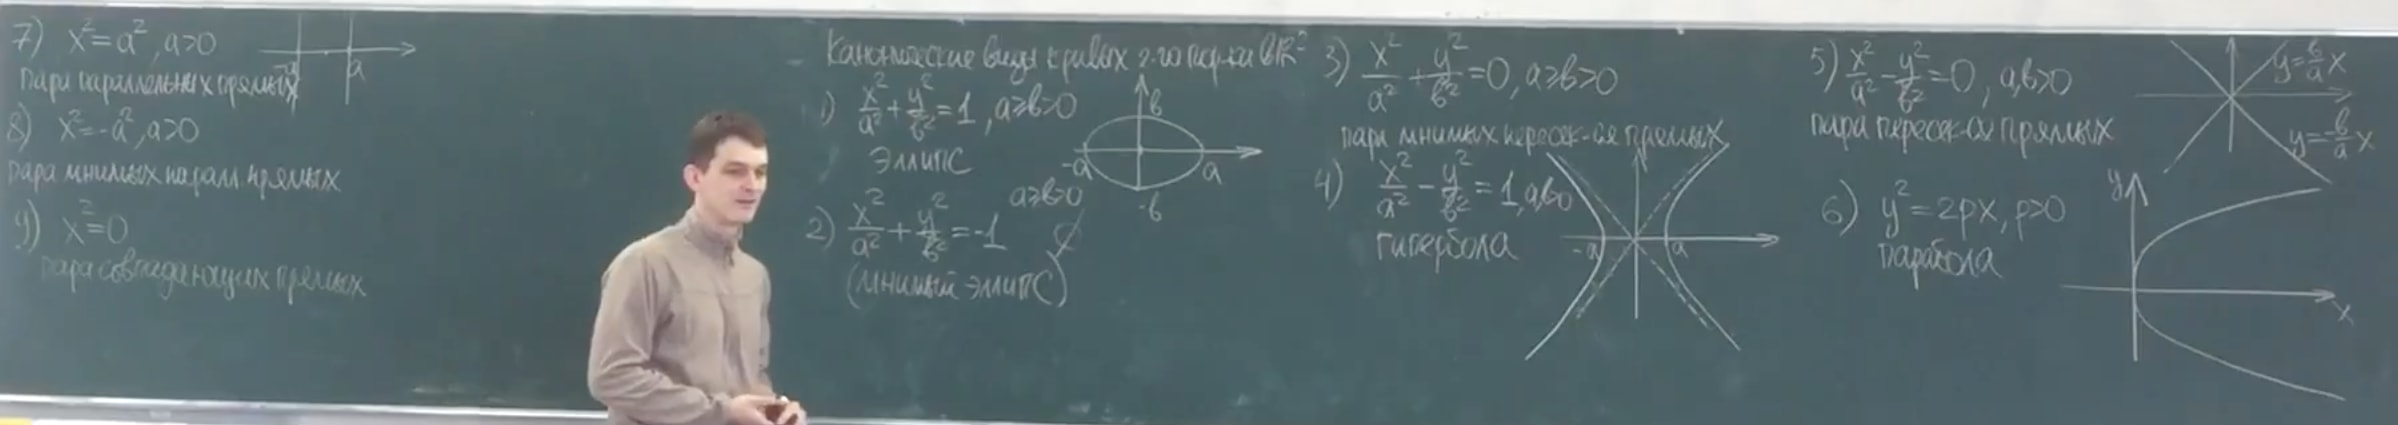
\includegraphics[width=19cm,height=15cm,keepaspectratio]{example2.jpg}

\subsection{Канонические виды поверхностей второго порядка в $\mathbb{R}^3$}

1) $\frac{x^2}{a^2} + \frac{y^2}{b^2} + \frac{z^2}{c^2} = 1, a \geqslant b \geqslant c > 0$ -- эллипсоид

\vspace{\baselineskip}
2) $\frac{x^2}{a^2} + \frac{y^2}{b^2} + \frac{z^2}{c^2} = -1$ -- мнимый эллипсоид

\vspace{\baselineskip}
3) $\frac{x^2}{a^2} + \frac{y^2}{b^2} + \frac{z^2}{c^2} = 0$ -- вырожденный эллипсоид

\vspace{\baselineskip}
4) $\frac{x^2}{a^2} + \frac{y^2}{b^2} - \frac{z^2}{c^2} = 1, a \geqslant b > 0, c > 0$ -- однополостный гиперболоид

\vspace{\baselineskip}
5) $\frac{x^2}{a^2} + \frac{y^2}{b^2} - \frac{z^2}{c^2} = -1, a \geqslant b > 0, c > 0$ -- двуполостный гиперболоид

\vspace{\baselineskip}
6) $\frac{x^2}{a^2} + \frac{y^2}{b^2} - \frac{z^2}{c^2} = 0, a \geqslant b > 0, c > 0$ -- эллиптический конус

\vspace{\baselineskip}
7) $\frac{x^2}{a^2} + \frac{y^2}{b^2} = 2z$ -- эллиптический параболоид

\vspace{\baselineskip}
8) $\frac{x^2}{a^2} - \frac{y^2}{b^2} = 2z$ -- гиперболический параболоид

\vspace{\baselineskip}
9) $\frac{x^2}{a^2} + \frac{y^2}{b^2} = 1, a \geqslant b > 0$ -- эллиптический цилиндр

\vspace{\baselineskip}
10) $\frac{x^2}{a^2} + \frac{y^2}{b^2} = -1$ -- мнимый эллиптический цилиндр

\vspace{\baselineskip}
11) $\frac{x^2}{a^2} - \frac{y^2}{b^2} = 1$ -- гиперболический цилиндр

\vspace{\baselineskip}
12) $y^2 = 2px, p > 0$ -- параболический цилиндр

\vspace{\baselineskip}
13) $\frac{x^2}{a^2} - \frac{y^2}{b^2} = 0$ -- пара пересекающихся плоскостей

\vspace{\baselineskip}
14) $\frac{x^2}{a^2} + \frac{y^2}{b^2} = 0$ -- пара мнимых пересекающихся плоскостей

\vspace{\baselineskip}
15) $y^2 = a^2, a \neq 0$ -- пара параллельных плоскостей

\vspace{\baselineskip}
16) $y^2 = -a^2, a \neq 0$ -- пара мнимых параллельных плоскостей

\vspace{\baselineskip}
17) $y^2 = 0$ -- пара совпадающих плоскостей


    \section{Лекция 7.06.2018}

\subsection{Эллипс}

$\frac{x^2}{a^2} + \frac{y^2}{b^2} = 1, a \geqslant b > 0$

\vspace{\baselineskip}
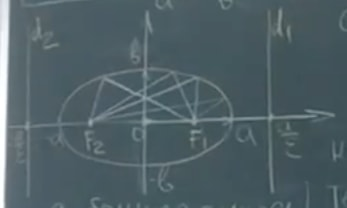
\includegraphics[width=10cm,height=15cm,keepaspectratio]{example3.jpg}

\vspace{\baselineskip}
$a$ -- большая полуось, $b$ -- малая полуось

$c = \sqrt[]{a^2 - b^2}$

$0 \leqslant c < a$

Точки $F_1(c, 0), F_2(-c, 0)$ называются \textit{фокусами} эллипса.

\vspace{\baselineskip}
\textbf{Теорема.} Точка $P$ лежит на эллипсе $\Leftrightarrow \rho(P, F_1) + \rho(P, F_2) = 2a$

\vspace{\baselineskip}
$\epsilon = \frac{c}{a}, 0 \leqslant \epsilon \leqslant 1$ -- эксцентралитет эллипса

\vspace{\baselineskip}
Прямые $d_1: x = \frac{a}{\epsilon}, d_2: x = -\frac{a}{\epsilon}$ называются \textit{директрисами} эллипса.

\vspace{\baselineskip}
\textbf{Теорема.} Точка $P$ лежит на эллипсе $\Leftrightarrow \frac{\rho(P, F_i)}{\rho(d_i)} = \epsilon$

\vspace{\baselineskip}
\textbf{\textit{Оптическое свойство эллипса:}} Лучи света, выпущенные из одного фокуса, после отражения от стенок собираются в другом фокусе.

\subsection{Гипербола}

$\frac{x^2}{a^2} - \frac{y^2}{b^2} = 1, a \geqslant b > 0$

\vspace{\baselineskip}
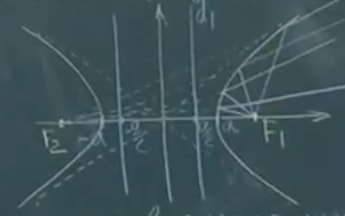
\includegraphics[width=10cm,height=15cm,keepaspectratio]{example4.jpg}

\vspace{\baselineskip}
$a$ -- действительная полуось, $b$ -- мнимая полуось

\vspace{\baselineskip}
$y = \frac{b}{a}x, y = - \frac{b}{a}x$ -- асимптоты

$c = \sqrt[]{a^2 + b^2}, c > a$

$F_1(c, 0), F_2(-c, 0)$ -- фокусы

\vspace{\baselineskip}
\textbf{Теорема.} $P$ лежит на гиперболе $\Leftrightarrow |\rho(P, F_1) - \rho(P, F_2)| = 2a$

\vspace{\baselineskip}
$\epsilon = \frac{c}{a}, \epsilon > 1$

\vspace{\baselineskip}
Директрисы: $d_1: x = \frac{a}{\epsilon}, d_2: x = -\frac{a}{\epsilon}$

\vspace{\baselineskip}
\textbf{Теорема.}  Точка $P$ лежит на гиперболе $\Leftrightarrow \frac{\rho(P, F_i)}{\rho(d_i)} = \epsilon$

\vspace{\baselineskip}
\textbf{\textit{Оптическое свойство гиперболы:}} Лучи света, выпущенные из одного фокуса, после отражения от стенок идут так, как будто они были выпущены из другого фокуса.

\subsection{Парабола}

$y^2 = 2px, p>0$

\vspace{\baselineskip}
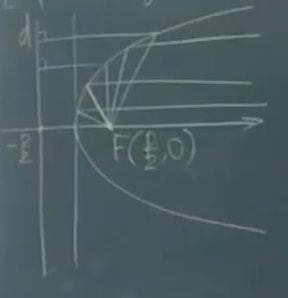
\includegraphics[width=10cm,height=15cm,keepaspectratio]{example5.jpg}

\vspace{\baselineskip}
Фокус: $F(\frac{p}{2}, 0)$

Директриса: $d: x = \frac{p}{2}$

$\epsilon = 1$

\vspace{\baselineskip}
\textbf{Теорема.} Точка $P$ лежит на гиперболе $\Leftrightarrow \rho(P, F) = \rho(P, d)$

\vspace{\baselineskip}
\textbf{\textit{Оптическое свойство параболы:}} Лучи света, выпущенные из фокуса, после отражения от стенок идут параллеьно оси $Ox$.

\vspace{\baselineskip}
Эллипс, гипербола и парабола называются кониками (или коническими сечениями)

\vspace{\baselineskip}
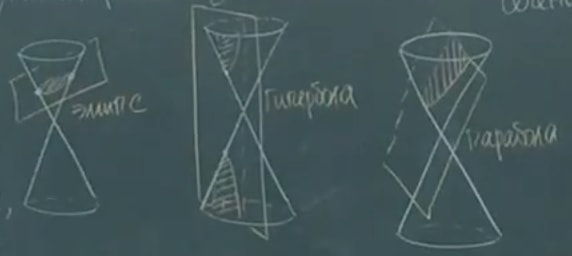
\includegraphics[width=10cm,height=15cm,keepaspectratio]{example6.jpg}

\subsection{Жорданова нормальная форма}

$V$ -- векторное пространство над полем $F$

$\varphi: V \rightarrow V$ -- линейный оператор

\vspace{\baselineskip}
\textbf{\textbf{Критерий диагонализуемости:}}

$\varphi$ диагонализуем $\Leftrightarrow$

1) $\chi_{\varphi} (t) = (t - \lambda_1)^{k_1} \dots (t = \lambda_s)^{k_s}$

2) $\forall \ i: k_i = dim V_{\lambda_i} (\varphi)$

\vspace{\baselineskip}
\textbf{Теорема (о Жордановой нормальной форме).} Пусть выполнено условие 1), т.е. $\chi_{\varphi} (t) = (t - \lambda_1)^{k_1} \dots (t - \lambda_s)^{k_s}$. Тогда $\exists$ базис $e$ в $V$, такой что \begin{equation*}A(\varphi, e) = \left(
\begin{array}{c|c|c|c|c}
  J^{m_1}_{\mu_1} & 0 & 0 & \dots & 0  \\
  \hline
  0 & J^{m_2}_{\mu_2} & 0 & \dots & 0  \\
  \hline
  0 & 0 & J^{m_3}_{\mu_3} & \dots & 0 \\
  \hline
  \vdots & \vdots & \vdots & \vdots & \vdots \\
  \hline
  0 & 0 & 0 & \dots & J^{m_p}_{\mu_p} \\
\end{array}
\right) (*)\end{equation*}

где $J^{m_i}_{\mu_i} = \begin{pmatrix} \mu_i & 1 & 0 & \dots & 0 \\ 0 & \mu_i & 1 & \dots & 0 \\ 0 & 0 & \mu_i & \dots & 0
\\ \vdots & \vdots & \vdots & \vdots & \vdots \\ 0 & 0 & 0 & \dots & \mu_i \end{pmatrix}$ -- Жорданова клетка порядка $m_i$ с собственным значением $\mu_i$

$\{\mu_1, \dots, \mu_p\} = Spec \varphi = \{\lambda_1, \dots, \lambda_p\}$

\vspace{\baselineskip}
Более того, вид $(*)$ определен однозначно с точностью до перестановки клеток.

\vspace{\baselineskip}
$\varphi \in L(V), \chi_{\varphi} (t) = (t - \lambda_1)^{k_1} \dots (t - \lambda_s)^{k_s}$

$\lambda \in Spec \varphi$

\vspace{\baselineskip}
\textbf{Определение.} Вектор $v \in V$ называется \textit{корневым вектором линейного оператора} $\varphi$, отвечающим собственному значению $\lambda$, если $\exists \ m \geqslant 0$, такое что $(\varphi - \lambda \cdot Id)^m v = 0$.

При этом наименьшее такое $m$ называется \textit{высотой} корневого вектора $v$. Обозначение: $ht(v)$

\vspace{\baselineskip}
$ht(v) = 0 \Leftrightarrow v = 0$

$ht(v) = 1 \Leftrightarrow (\varphi - \lambda \cdot Id) v = 0 \Leftrightarrow \varphi(v) = \lambda v \Leftrightarrow v$ -- собственный вектор с собственным значением $\lambda$

\vspace{\baselineskip}
$V^{\lambda} (\varphi)$ -- множество всех корневых векторов, отвечающих собственному значению $\lambda$

\vspace{\baselineskip}
\textbf{\textit{Упражнение.}} $V^{\lambda} (\varphi)$ -- подпространство в $V$

\vspace{\baselineskip}
\textbf{Определение.} $V^{\lambda} (\varphi)$ называется \textit{корневым подпространством}, отвечающим собственному значению $\lambda$

\vspace{\baselineskip}
\textbf{Замечание.} $V_{\lambda} (\varphi) \subseteq V^{\lambda} (\varphi)$

\vspace{\baselineskip}
Пример.

$V = F[x]_{\leqslant n}, char F = 0$

$\varphi: f \rightarrow f'$

$\chi_{\varphi}(t) = t^{n+1}, Spec \varphi = \{0\}$

$V^0 (\varphi) = V$

$F \in V \Rightarrow deg(f) = k \Leftrightarrow ht(f) = k + 1$

\vspace{\baselineskip}
\textbf{Факты.}

1) $V^{\lambda} (\varphi) \ \varphi$-инвариантно

2) $dim V^{\lambda} (\varphi) = $ алгебраической кратности собственного значения $\lambda$

3) Если $\lambda_1, \dots, \lambda_k \in Spec \varphi, \lambda_i \neq \lambda_j$ при $i \neq j$, то $V^{\lambda_1} (\varphi) \dots V^{\lambda_k} (\varphi)$ линейно независимы

\vspace{\baselineskip}
\textbf{Следствие.} Если $\chi_{\varphi} (t) = (t - \lambda_1)^{k_1} \dots (t - \lambda_s)^{k_s}$, то $V = V^{\lambda_1} (\varphi) \oplus \dots \oplus V^{\lambda_s} (\varphi)$

\vspace{\baselineskip}
Если $e_i$ -- базис в $V^{\lambda} (\varphi)$ и $e = e_1 \sqcup e_1 \sqcup \dots \sqcup e_s$, то \begin{equation*}A(\varphi, e) = \left(
\begin{array}{c|c|c|c|c}
  A_1 & 0 & 0 & \dots & 0  \\
  \hline
  0 & A_2 & 0 & \dots & 0  \\
  \hline
  0 & 0 & A_3 & \dots & 0 \\
  \hline
  \vdots & \vdots & \vdots & \vdots & \vdots \\
  \hline
  0 & 0 & 0 & \dots & A_s \\
\end{array}
\right)\end{equation*}

$A_i = A(\varphi|_{V^{\lambda_i} (\varphi)}, e_i)$

$\Rightarrow$ доказательство теоремы о ЖНФ сводится к случаю $V = V^{\lambda_i} (\varphi)$

Далее считаем, что $Spec \varphi = \{ \lambda\}, \chi_{\varphi} (t) = (t - \lambda)^n, n = dim V$

$V = V^{\lambda} (\varphi)$

Полагая $\psi = \varphi - \lambda \cdot Id$, получаем $\chi_{\psi} (t) = t^n, Spec \psi = \{0\}, V = V^0 (\psi)$

Далее считаем $Spec \varphi = \{0\}$

\vspace{\baselineskip}
\textbf{Определение.} Линейный оператор называется \textit{нильпотентным}, если $\exists m \in \mathbb{N}$, такой что $\varphi^m = 0$

\vspace{\baselineskip}
Фиксируем наименьший $m$, такой что $\varphi^m = 0$. Имеем $0 = Ker \varphi^0 \subseteq \overbrace{Ker \varphi^1}^{собственное \ подпространство} \subseteq Ker \varphi^2 \subseteq \dots \subseteq Ker \varphi^m = V$


    \section{Лекция 14.06.2018}

$V$ -- векторное пространство над $F$

$\varphi: V \rightarrow V$ -- линейный оператор

$\chi_{\varphi} (t) = (t - \lambda_1)^{k_1} \dots (t - \lambda_s)^{k_s}$

$i \in \{1, \dots, s\} \Rightarrow V^{\lambda_i} (\varphi)$ -- корневое подпространство

$dim V^{\lambda_i} (\varphi) = k_i$

$V = V^{\lambda_1} (\varphi) \oplus \dots \oplus V^{\lambda_s} (\varphi)$

$\varphi_i = (\varphi - \lambda_i \cdot Id) | _{V^{\lambda_i} (\varphi)}$

$Spec \varphi_i = \{0\}$

$\varphi_i^{k_i} = 0$

\vspace{\baselineskip}
\textbf{Определение.} Линейный оператор $\varphi$ называется \textit{нильпотентным}, если $\exists \ m \in \NN$, такой что $\varphi^m > 0$.

\vspace{\baselineskip}
Пусть $m \in \NN$ наименьшее с таким свойством.

$\{0\} = Ker \varphi \subsetneqq Ker \varphi^1 \subsetneqq Ker \varphi^2 \subsetneqq \dots \subsetneqq Ker \varphi^m = V$

$d_i = dim Ker \varphi^i$

$0 = d_0 < d_1 < d_2 < \dots < d_m = n = dim V$

$v \in V, ht(v) = k$

\vspace{\baselineskip}
\textbf{Лемма.} Векторы $v, \varphi(v), \dots, \varphi^{k-1}(v)$ линейно независимы.

\vspace{\baselineskip}
$C(v) = <v, \varphi(v), \dots, \varphi^{k-1} (v)>$

\vspace{\baselineskip}
\textbf{Определение.} $C(v)$ называется \textit{циклическим подпространством}, порожденным вектором $v$.

\vspace{\baselineskip}
$C(v) \ \varphi$-инвариантно

\vspace{\baselineskip}
$B(v) = (\varphi^{k-1} (\varphi), \dots, \varphi(v), v)$ -- базис в $C(v)$

\vspace{\baselineskip}
Матрица линейного оператора $\varphi|_{C(v)}$ в базисе $B(v)$ равна \begin{equation*}\begin{pmatrix} 0 & 1 & 0 & \dots & 0 & 0 \\ 0 & 0 & 1 & \dots & 0 & 0 \\ 0 & 0 & 1 & \dots & 0 & 0 \\ \vdots & \vdots & \vdots & \ddots & \vdots & \vdots \\ 0 & 0 & 0 & \dots & 0 & 1 \\ 0 & 0 & 0 & \dots & 0 & 0 \\ \end{pmatrix}\end{equation*}

Вывод: достаточно разложить $V$ в прямую сумму циклических подпространств.

\subsection{Метод построения жорданова базиса}

\vspace{\baselineskip}
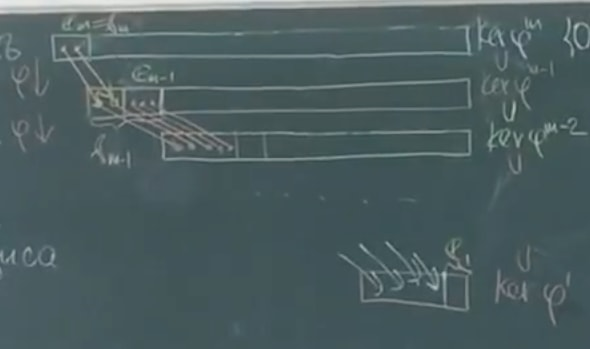
\includegraphics[width=10cm,height=15cm,keepaspectratio]{example7.jpg}

\vspace{\baselineskip}
\underline{Шаг 1.} Выберем линейно независимый набор $e_m \subseteq Ker \varphi^m$, такой что $Ker \varphi^m = <e_m> \oplus Ker \varphi^{m-1}$

Положим $f_m = e_m$

\vspace{\baselineskip}
\underline{Шаг 2.} Выберем линейно независимый набор $e_{m - 1} \subseteq Ker \varphi^{m-1}$, такой что $Ker \varphi^{m-1} = <\varphi(f_m)> \oplus <e_{m-1}> \oplus Ker \varphi^{m-2}$

Положим $f_{m-1} = \varphi(f_m) \cup e_{m-1}$

\vspace{\baselineskip}
(и так далее)

\vspace{\baselineskip}
\underline{Шаг $m$.} Выберем линейно независимый набор $e_1 \subseteq Ker \varphi$, такой что $Ker \varphi = <\varphi(f_2)> \oplus <e_1>$

\vspace{\baselineskip}
На выходе получаем наборы $e_m, \dots, e_1$

Положим $e = e_m \cup \dots \cup e_1$

\vspace{\baselineskip}
\textbf{Теорема.} 1) $V = \oplus_{e' \in e} C(e')$

2) $\cup_{e' \in e} B(e')$ -- жорданов базис для $\varphi$

\vspace{\baselineskip}
Пусть $c_k$ число жордановых клеток размера $k$

$c_k = |e_k|$

$Ker \varphi^k = <\varphi(f_{k+1})> \oplus <e_k> \oplus Ker \varphi^{k-1}$

$d_k = \overbrace{|\varphi(f_{k+1})|}^{= d_{k+1} - d_k} + c_k + d_{k-1}$

$d_k = d_{k+1} - d_k + c_k + d_{k - 1}$

$c_k = 2d_k - d_{k-1} - d_{k+1}$

\subsection{Полуторалинейные формы и эрмитовы пространства}

\vspace{\baselineskip}
билинейная форма

$\downarrow$

симметричная билинейная форма

$\downarrow$

квадратичная форма

$\downarrow$

положительно определенная квадратичная форма (над $\RR$)

$\downarrow$

евклидово пространство (над $\RR$)

\vspace{\baselineskip}
\textbf{Определение.} \textit{Полуторалинейная форма (1,5-линейная)} на векторном пространстве $V$ над $\CC$ -- это отображение $\beta: V \times V \rightarrow \CC$, такое что

1) Полулинейность по первому аргументу

$\beta(\alpha_1 x_1 + \alpha_2 x_2, y) = \overline{\alpha_1} \beta (x_1, y) + \overline{\alpha_2} \beta (x_2, y)$

2) Линейность по второму аргументу

\vspace{\baselineskip}
В координатах $x = \begin{pmatrix} x_1 \\ \vdots \\ x_{n} \end{pmatrix}, y = \begin{pmatrix} y_1 \\ \vdots \\ y_{n} \end{pmatrix}$

$\beta(x, y) = (\overline{x_1}, \dots, \overline{x_n}) B \begin{pmatrix} y_1 \\ \vdots \\ y_{n} \end{pmatrix}$

\vspace{\baselineskip}
Формула изменения матрицы 1,5-линейной формы:

$B' = C^* B C$

$C^* = \overline{C}^T = (\overline{c_{ji}})$

\vspace{\baselineskip}
\textbf{Определение.} 1,5-линейная форма называется \textit{эрмитовой}, если $\beta(y, x) = \overline{\beta(x, y)}$

\vspace{\baselineskip}
$\beta(x, x) = \overline{\beta(x, x)} \Rightarrow \beta(x, x) \in \RR$

$Q(x) = \beta(x, x)$ -- эрмитова квадратичная форма

\vspace{\baselineskip}
$Q:V \rightarrow R$

\textbf{Теорема о нормальном виде.} $Q$ -- эрмитова квадратичная форма $\Rightarrow \exists$ базис, такой что $Q(x) = |x_1|^2 + \dots + |x_k|^2 - |x_{k+1}|^2 - \dots - |x_{k + s}|^2$

\vspace{\baselineskip}
\textbf{Определение.} \textit{Эрмитово пространство} -- это векторное пространство над $\CC$, на котором задано скалярное произведение, то есть положительно определенная эрмитова 1,5-линейная форма.

\vspace{\baselineskip}
1,5-линейная форма

$\downarrow$

эрмитова форма

$\downarrow$

эрмитова квадратичная форма

$\downarrow$

положительно определенная эрмитова квадратичная форма (над $\CC$)

$\downarrow$

эрмитово пространство (над $\CC$)

\vspace{\baselineskip}
Длина: $|x| = \sqrt[]{(x, x)}$

Неравенство Коши-Буняковского

Неравенство треугольника

Ортогональность

Ортогональное дополнение

$U$ -- подпространство в $V \Rightarrow V = U \oplus U^{\bot}$

Ортонормированный базис

\vspace{\baselineskip}
$e, e'$ -- два ортогональных базиса, $e' = e \cdot C$

$C$ -- унитарная матрица

$C^{-1} = C^*$

\vspace{\baselineskip}
\textbf{Линейный операторы в эрмитовых пространствах}

1) самосопряженный $(\varphi(x), y) = (x, \varphi(y))$

2) унитарный $(\varphi(x), \varphi(y)) = \varphi(x, y)$

\vspace{\baselineskip}
\textbf{Теорема.} 1) $\varphi$ -- самосопряженный $\Rightarrow \exists$ ортонормированный базис из собственных векторов; $Spec \varphi \subseteq \RR$

2) $\varphi$ -- унитарный оператор $\Rightarrow \exists$ ортонормированный базис из собственных векторов

$\lambda \in Spec f \Rightarrow |\lambda| = 1$

\vspace{\baselineskip}
Аналогичное сингулярное разложение

\vspace{\baselineskip}
$A \in Mat_{m \times n} (\CC) \Rightarrow \exists$ унитарная матрица $U \in M_m(\CC), V \in M_n (\CC)$, такие что $A = U \Sigma V^*$

$\Sigma = \begin{pmatrix} \sigma_1 & 0 & 0 & 0 & 0 & 0 & 0 \\  0 & \sigma_2 & 0 & 0 & 0 & 0 & 0 \\ 0 & 0 & \ddots & 0 & 0 & 0 & 0 \\ 0 & 0 & 0 & \sigma_r & 0 & 0 & 0 \\ 0 & 0 & 0 & 0 & 0 & 0 & 0 \\ 0 & 0 & 0 & 0 & 0 & \ddots & 0 \\ 0 & 0 & 0 & 0 & 0 & 0 & 0 \end{pmatrix}, \sigma_i \in \RR, \sigma_1 \geqslant \dots \geqslant \sigma_r > 0, \sigma_i$ определено однозначно 























\end{document}
\end{document}
